% Options for packages loaded elsewhere
\PassOptionsToPackage{unicode}{hyperref}
\PassOptionsToPackage{hyphens}{url}
%
\documentclass[
  12pt,dutch,coursenotes]{book}
\usepackage{lmodern}
\usepackage{amssymb,amsmath}
\usepackage{ifxetex,ifluatex}
\ifnum 0\ifxetex 1\fi\ifluatex 1\fi=0 % if pdftex
  \usepackage[T1]{fontenc}
  \usepackage[utf8]{inputenc}
  \usepackage{textcomp} % provide euro and other symbols
\else % if luatex or xetex
  \usepackage{unicode-math}
  \defaultfontfeatures{Scale=MatchLowercase}
  \defaultfontfeatures[\rmfamily]{Ligatures=TeX,Scale=1}
\fi
% Use upquote if available, for straight quotes in verbatim environments
\IfFileExists{upquote.sty}{\usepackage{upquote}}{}
\IfFileExists{microtype.sty}{% use microtype if available
  \usepackage[]{microtype}
  \UseMicrotypeSet[protrusion]{basicmath} % disable protrusion for tt fonts
}{}
\makeatletter
\@ifundefined{KOMAClassName}{% if non-KOMA class
  \IfFileExists{parskip.sty}{%
    \usepackage{parskip}
  }{% else
    \setlength{\parindent}{0pt}
    \setlength{\parskip}{6pt plus 2pt minus 1pt}}
}{% if KOMA class
  \KOMAoptions{parskip=half}}
\makeatother
\usepackage{xcolor}
\IfFileExists{xurl.sty}{\usepackage{xurl}}{} % add URL line breaks if available
\IfFileExists{bookmark.sty}{\usepackage{bookmark}}{\usepackage{hyperref}}
\hypersetup{
  pdftitle={Cursus Statistiek 2020-2021},
  pdfauthor={Lieven Clement},
  hidelinks,
  pdfcreator={LaTeX via pandoc}}
\urlstyle{same} % disable monospaced font for URLs
\usepackage{color}
\usepackage{fancyvrb}
\newcommand{\VerbBar}{|}
\newcommand{\VERB}{\Verb[commandchars=\\\{\}]}
\DefineVerbatimEnvironment{Highlighting}{Verbatim}{commandchars=\\\{\}}
% Add ',fontsize=\small' for more characters per line
\usepackage{framed}
\definecolor{shadecolor}{RGB}{248,248,248}
\newenvironment{Shaded}{\begin{snugshade}}{\end{snugshade}}
\newcommand{\AlertTok}[1]{\textcolor[rgb]{0.94,0.16,0.16}{#1}}
\newcommand{\AnnotationTok}[1]{\textcolor[rgb]{0.56,0.35,0.01}{\textbf{\textit{#1}}}}
\newcommand{\AttributeTok}[1]{\textcolor[rgb]{0.77,0.63,0.00}{#1}}
\newcommand{\BaseNTok}[1]{\textcolor[rgb]{0.00,0.00,0.81}{#1}}
\newcommand{\BuiltInTok}[1]{#1}
\newcommand{\CharTok}[1]{\textcolor[rgb]{0.31,0.60,0.02}{#1}}
\newcommand{\CommentTok}[1]{\textcolor[rgb]{0.56,0.35,0.01}{\textit{#1}}}
\newcommand{\CommentVarTok}[1]{\textcolor[rgb]{0.56,0.35,0.01}{\textbf{\textit{#1}}}}
\newcommand{\ConstantTok}[1]{\textcolor[rgb]{0.00,0.00,0.00}{#1}}
\newcommand{\ControlFlowTok}[1]{\textcolor[rgb]{0.13,0.29,0.53}{\textbf{#1}}}
\newcommand{\DataTypeTok}[1]{\textcolor[rgb]{0.13,0.29,0.53}{#1}}
\newcommand{\DecValTok}[1]{\textcolor[rgb]{0.00,0.00,0.81}{#1}}
\newcommand{\DocumentationTok}[1]{\textcolor[rgb]{0.56,0.35,0.01}{\textbf{\textit{#1}}}}
\newcommand{\ErrorTok}[1]{\textcolor[rgb]{0.64,0.00,0.00}{\textbf{#1}}}
\newcommand{\ExtensionTok}[1]{#1}
\newcommand{\FloatTok}[1]{\textcolor[rgb]{0.00,0.00,0.81}{#1}}
\newcommand{\FunctionTok}[1]{\textcolor[rgb]{0.00,0.00,0.00}{#1}}
\newcommand{\ImportTok}[1]{#1}
\newcommand{\InformationTok}[1]{\textcolor[rgb]{0.56,0.35,0.01}{\textbf{\textit{#1}}}}
\newcommand{\KeywordTok}[1]{\textcolor[rgb]{0.13,0.29,0.53}{\textbf{#1}}}
\newcommand{\NormalTok}[1]{#1}
\newcommand{\OperatorTok}[1]{\textcolor[rgb]{0.81,0.36,0.00}{\textbf{#1}}}
\newcommand{\OtherTok}[1]{\textcolor[rgb]{0.56,0.35,0.01}{#1}}
\newcommand{\PreprocessorTok}[1]{\textcolor[rgb]{0.56,0.35,0.01}{\textit{#1}}}
\newcommand{\RegionMarkerTok}[1]{#1}
\newcommand{\SpecialCharTok}[1]{\textcolor[rgb]{0.00,0.00,0.00}{#1}}
\newcommand{\SpecialStringTok}[1]{\textcolor[rgb]{0.31,0.60,0.02}{#1}}
\newcommand{\StringTok}[1]{\textcolor[rgb]{0.31,0.60,0.02}{#1}}
\newcommand{\VariableTok}[1]{\textcolor[rgb]{0.00,0.00,0.00}{#1}}
\newcommand{\VerbatimStringTok}[1]{\textcolor[rgb]{0.31,0.60,0.02}{#1}}
\newcommand{\WarningTok}[1]{\textcolor[rgb]{0.56,0.35,0.01}{\textbf{\textit{#1}}}}
\usepackage{longtable,booktabs}
% Correct order of tables after \paragraph or \subparagraph
\usepackage{etoolbox}
\makeatletter
\patchcmd\longtable{\par}{\if@noskipsec\mbox{}\fi\par}{}{}
\makeatother
% Allow footnotes in longtable head/foot
\IfFileExists{footnotehyper.sty}{\usepackage{footnotehyper}}{\usepackage{footnote}}
\makesavenoteenv{longtable}
\usepackage{graphicx}
\makeatletter
\def\maxwidth{\ifdim\Gin@nat@width>\linewidth\linewidth\else\Gin@nat@width\fi}
\def\maxheight{\ifdim\Gin@nat@height>\textheight\textheight\else\Gin@nat@height\fi}
\makeatother
% Scale images if necessary, so that they will not overflow the page
% margins by default, and it is still possible to overwrite the defaults
% using explicit options in \includegraphics[width, height, ...]{}
\setkeys{Gin}{width=\maxwidth,height=\maxheight,keepaspectratio}
% Set default figure placement to htbp
\makeatletter
\def\fps@figure{htbp}
\makeatother
\setlength{\emergencystretch}{3em} % prevent overfull lines
\providecommand{\tightlist}{%
  \setlength{\itemsep}{0pt}\setlength{\parskip}{0pt}}
\setcounter{secnumdepth}{5}
\usepackage{booktabs}
\usepackage{amsthm}
\usepackage{float}
\usepackage{fontspec}
%\setmainfont{cmunrm.otf}
\makeatletter
\def\thm@space@setup{%
  \thm@preskip=8pt plus 2pt minus 4pt
  \thm@postskip=\thm@preskip
}
\makeatother
\hypersetup{colorlinks=true,urlcolor=blue,citecolor=blue,linkcolor=blue,linktoc=page}
\urlstyle{same}
\usepackage{a4wide}
\setlength{\parindent}{0in}
\setlength{\parskip}{2ex}
\usepackage[dutch]{babel}
% grootte van de pagina
\setlength{\topmargin}{-0.25in}
\setlength{\oddsidemargin}{0.25in}					    
\setlength{\evensidemargin}{0.25in}
\setlength{\textwidth}{6.0in}
\setlength{\textheight}{9.0in}
\ifluatex
  \usepackage{selnolig}  % disable illegal ligatures
\fi
\usepackage[]{natbib}
\bibliographystyle{apalike}

\title{Cursus Statistiek 2020-2021}
\author{Lieven Clement}
\date{2020-09-21}

\usepackage{amsthm}
\newtheorem{theorem}{Theorema}[chapter]
\newtheorem{lemma}{Lemma}[chapter]
\newtheorem{corollary}{Corollary}[chapter]
\newtheorem{proposition}{Eigenschap}[chapter]
\newtheorem{conjecture}{Conjecture}[chapter]
\theoremstyle{definition}
\newtheorem{definition}{Definitie}[chapter]
\theoremstyle{definition}
\newtheorem{example}{Voorbeeld}[chapter]
\theoremstyle{definition}
\newtheorem{exercise}{Oefening}[chapter]
\theoremstyle{remark}
\newtheorem*{remark}{Opmerking }
\newtheorem*{solution}{Oplossing }
\begin{document}
\maketitle

{
\setcounter{tocdepth}{1}
\tableofcontents
}
\hypertarget{woord-vooraf}{%
\chapter*{Woord vooraf}\label{woord-vooraf}}
\addcontentsline{toc}{chapter}{Woord vooraf}

Zoals steeds heeft het herwerken van de cursus heel wat voeten in de aarde. Gelukkig kon ik me hierbij baseren op cursusmateriaal van collega's. In het bijzonder wens ik prof. Stijn Vansteelandt\footnote{die vroeger dit opleidingsonderdeel verzorgde}, prof. Olivier Thas\footnote{Opleidingsonderdeel ``Statistische Dataverwerking'', Bachelor in de Bio-ingenieurswetenschappen, UGent} en prof. Geert Verbeke\footnote{Opleidingsonderdeel ``Beginselen van biostatistiek'', Bachelor Biomedical Sciences, KU Leuven} te bedanken voor het delen van hun cursusmateriaal en de stimulerende discussies rond statistiekonderwijs. Daarnaast was het ook een nieuwe ervaring om een volledige cursus te ontwikkelen binnen het statistische opensource software pakket R via het fantastische bookdown package van Yihui Xie.

Lieven, September 2018

In de zomer 2020 hebben we de transitie gemaakt van een online ebook naar een volledig online course.
Hierbij integreren we alle materiaal voor de cursus en de oefeningen in het Dodona leerplatform.
De cursus kan volledig in dit platform worden doorlopen aan de hand van leesopdrachten voor de theorie en d.m.v. oefeningen waarvan de code automatisch kan worden beoordeeld.
Dit huzarenstukje was uiteraard niet mogelijk zonder de hulp van een bijzonder gedreven team.

Eerst en vooral wil ik het Dodona team bedanken om me herhaaldelijk aan te sporen om ook statistiekonderwijs via Dodona te verstrekken. Prof.~Peter Dawyndt en Dr.~Bart Mesure hebben samen met hun team een indrukwekkend platform ontwikkelt voor het doceren van programmeertalen.

Daarnaast heeft Charlotte Van Petegem het platform ook voor statistiek onderwijs unlocked door de ontwikkeling van een R-judge waarbij R code automatisch kan worden beoordeeld.

De Faculteit Wetenschappen van de Universiteit van Gent heeft het me d.m.v. een onderwijs en innovatieproject mogelijk gemaakt om in augustus 2020 een team van enthousiaste jobstudenten: Gust Bogaert, Luca Renders, Stijn Vandenbulcke en Victor Verstraelen aan te werven die in een maand tijd twee modules (Introductie tot R en Data exploratie en Data Visualisatie in R) in Dodona hebben geïmplementeerd. Dat was mede mogelijk omdat we van prof. Rafael Irizarry de toestemming kregen om de broncode van zijn boek Introduction to Data Science en alle youtube videos te integreren in deze modules.

Onder impuls van mijn team jonge enthousiaste wolven hebben we het aangedurfd om midden september 2020 ook mijn volledige cursus Statistiek in Dodona onder te gaan brengen. In deze bevreemdende covid-19 tijden lijkt me dit de ultieme manier om de stof zo goed mogelijk interactief en volledig online aan te bieden.
Ik kan het schitterende team van jobstudenten en het voltallige Dodona team niet voldoende bedanken, jullie gaven me vleugels!

Daarnaast wil ik ook mijn familie bedanken voor hun geduld en nooit aflatende steun tijdens de ontwikkeling van deze cursus.

Lieven, September 2020

\hypertarget{links}{%
\chapter*{Links}\label{links}}
\addcontentsline{toc}{chapter}{Links}

\begin{itemize}
\item
  De volledig interactieve versie van deze cursus is beschikbaar op \url{https://dodona.ugent.be/nl/courses/374/}
\item
  Een html versie van de cursus is beschikbaar op \url{https://statomics.github.io/sbc20/} waardoor alle voorbeelden en code in deze cursus makkelijk in R kunnen worden gereproduceerd, wat handig kan zijn wanneer je zelf r-markdown scripts ontwikkeld.
\item
  Een pdf versie van de cursus is beschikbaar op \url{https://statomics.github.io/sbc20/Statistiek_2020_2021.pdf}
\item
  Voor een introductie tot R en Data Visualisatie raden we de eerste twee delen aan van het ebook \url{https://rafalab.github.io/dsbook/} aan van prof. Raphael Irizarry. Volledig interactieve Dodona cursussen van deze twee delen vind je terug op Statistiek Introductie tot R: \url{https://dodona.ugent.be/nl/courses/375/} en Statistiek: Data Exploration and Visualisation in R: \url{https://dodona.ugent.be/nl/courses/376/}.
\end{itemize}

\hypertarget{inleiding}{%
\chapter{Inleiding}\label{inleiding}}

link naar playlist met kennisclips:
\href{https://www.youtube.com/playlist?list=PLZH1hP8_LbJIk4G2AZYYKvgZLjRR-1-Iw}{Kennisclips Hoofdstuk1}

De meeste vragen in de levenswetenschappen kunnen slechts beantwoord worden door gegevens te verzamelen en te analyseren, bijvoorbeeld:

\begin{itemize}
\tightlist
\item
  Voor welke genen verschilt het expressieniveau in kanker en normaal weefsel?
\item
  Kwaliteitscontrole: wijkt de concentratie van een chemisch product af van wat er op het label wordt vermeld?\\
\item
  Wat is de invloed van regelmatig joggen op bloeddruk?
\item
  Is er een relatie tussen zweetgeur en de samenstelling van de microbiële gemeenschap onder de oksel?
\end{itemize}

Bij onderzoek naar biologische processen moet men zich realiseren dat uitkomsten aan variatie onderhevig zijn. Aspirine is bijvoorbeeld niet bij iedereen even effectief om hoofdpijn te verzachten zodat de uitkomst voor een persoon met en zonder inname van aspirine meestal niet exact te voorspellen valt. Dit wordt mede veroorzaakt door het feit dat mensen verschillen in gewicht, ziektegraad, gevoeligheid voor een stof, \ldots{} Bovendien reageert een persoon vaak anders op een stof naargelang hij moe of uitgerust is, het middel 's morgens of `s avonds inneemt, voor of na het eten, op geregelde tijdstippen of met onregelmatige intervallen, \ldots{} En zelfs al mocht een bepaalde stof voor iedereen even effectief zijn, dan nog is het zo dat verschillende metingen voor een zelfde persoon zelden gelijk.
De aanwezigheid van die biologische variabiliteit is bijzonder opvallend in de context van roken: de schadelijke gevolgen van roken op longkanker en hartaandoeningen zijn intussen goed gekend, maar nagenoeg iedereen kent wel iemand die gans zijn leven gerookt heeft en desondanks meer dan 80 jaar oud geworden is.

Precies omwille van die biologische variabiliteit is het moeilijk om wetenschappelijke vragen goed te beantwoorden en zal men zelden onmiddellijk het antwoord zien na het bekijken van ruwe gegevens. Onderzoekers in de fysiologie, bijvoorbeeld, gaan vaak na wat het effect is van een bepaalde substantie (bijvoorbeeld, een geneesmiddel, hormoon of toxine) op experimentele dieren (bijvoorbeeld, ratten of ook in vitro weefselpreparaten). Dit effect wordt bestudeerd door verschillen in respons te meten tussen dieren geïnjecteerd met de substantie en controledieren die werden geïnjecteerd met een inactieve zoutoplossing. Omwille van biologische variatie zullen een aantal dieren die geïnjecteerd werden met lage dosissen van de toxische stof, het er vaak beter van af brengen dan sommige controledieren. Hierdoor kunnen geobserveerde effecten zowel toevallig zijn als wijzen op een systematisch effect. Bovendien moeten we ons afvragen of de controlegroep en de met substantie-geïnjecteerde groep een vergelijkbare gezondheid hebben. Zo niet, dan zou een mogelijk verschil in respons ook mede hierdoor verklaard kunnen worden.

Het doel van statistiek is precies om orde te scheppen in de chaos door duidelijk te maken hoeveel variatie op de gegevens toe te schrijven valt aan systematische verschillen (bijvoorbeeld, door het al dan niet inspuiten van een bepaalde substantie) en hoeveel aan toeval of biologische variatie.

Statistiek is immers de wetenschap rond verzamelen, exploreren en analyseren van data. Ze laat toe

\begin{itemize}
\tightlist
\item
  om tot een goede proefopzet te komen,
\item
  om te leren uit data en
\item
  om hierbij variabiliteit en onzekerheid te

  \begin{itemize}
  \tightlist
  \item
    kwantificeren
  \item
    controleren
  \item
    rapporteren
  \end{itemize}
\item
  d.m.v. statistische besluitvorming modellen op een formele wijze te toetsen aan de data.
\end{itemize}

Ze vervult daarom een belangrijke rol in zowat alle wetenschappen. Zie ondermeer de populaire column `'points of significance'' in Nature Methods. (\url{http://blogs.nature.com/methagora/2013/08/giving_statistics_the_attention_it_deserves.html})

In deze inleiding situeren we Statistiek in de Wetenschappelijke Methode.

\hypertarget{sec:wetMeth}{%
\section{De Wetenschappelijke Methode}\label{sec:wetMeth}}

Het doel van wetenschap is het begrijpen van de natuur (van het allerkleinste tot het allergrootste, van vroeger en nu tot in de toekomst). De \emph{Wetenschappelijke Methode} is de methodiek die vandaag de dag algemeen aanvaard wordt om onze wetenschappelijke kennis van de natuur op te bouwen. Twee belangrijke pijlers van de Wetenschappelijke Methode zijn theorie en observatie. Een wetenschappelijke theorie voorspelt hoe een natuurlijk proces zich gedraagt. Observaties kunnen gebruikt worden om deze theorie te bevestigen of te ontkrachten. Een wetenschappelijke theorie kan dus nooit bewezen worden door observatie, maar kan wel ontkracht worden door observatie. Dit is het \emph{falcificatieprincipe} van de wetenschapsfilosoof Karl Popper (1902-1994).

De levenswetenschappen berusten op empirisch onderzoek omdat observaties nodig zijn om de kennis uit te breiden. Theorieën kunnen gepostuleerd worden zonder observatie (hoewel dit zelden gebeurt), maar de wetenschapsgemeenschap neemt ze typisch maar voor waar aan nadat de nieuwe theorieën aan observatie getoetst worden.

Figuur \ref{fig:wetMet} is een schematische weergave van de Wetenschappelijke Methode.

\begin{itemize}
\item
  De \emph{natuur} staat bovenaan de driehoek. Dit stelt het universum, de wereld, de werkelijkheid of de \emph{waarheid} voor, waarover de mens kennis wil verzamelen.
\item
  Een \emph{model} (of een \emph{theorie}) stelt een denkbeeld van een aspect van de natuur voor. Een model laat toe om voorspellingen, verder \emph{predicties} genoemd te maken over het gedrag van een aspect van de natuur. Hierbij wordt niet noodzakelijk een mathematisch model bedoeld, maar kan het ook een kwalitatieve beschrijving zijn van een aspect van de natuur (bv. insecticide behandeling van planten leidt tot een vermindering van het aantal schadelijke insecten op de planten en tot een verhoogde opbrengst van de oogst).
\item
  Via een \emph{wetenschappelijk experiment} worden \emph{data} uit de \emph{natuur} gehaald. Data vormen een manifestatie van het werkelijke gedrag van de natuur. Het experiment moet \emph{representatief} en \emph{reproduceerbaar} zijn
\item
  \emph{Statistische Besluitvorming} (Engels: \emph{statistical inference}) vormt de brug tussen het model van de natuur en de data uit de natuur. \emph{Statistische Besluitvorming} laat toe op een formele wijze het model te toetsen aan de data en te besluiten in welke mate de wetenschappelijke gemeenschap de theorie en het model voor waar mag aannemen.
\item
  Statistiek wordt ingeroepen omdat de \emph{Wetenschappelijke Methode} niet zonder doel gebruikt wordt. Wetenschappers hebben gedeeltelijke kennis van de natuur via een aantal modellen/theorieën, maar deze kennis doet nieuwe vragen ontstaan. Dit leidt tot een nieuwe \emph{onderzoeksvraag} (bijvoorbeeld: zorgt het gebruik van insecticiden voor minder schade van insecten aan de plant?), welke vervolgens verfijnd wordt in een nauwkeurig geformuleerde \emph{hypothese} (bijvoorbeeld: Het aantal aangetaste bladeren is gelijk voor onbehandelde en pesticide-behandelde planten). Een hypothese is zodanig geformuleerd dat ze door data kan verworpen worden indien de hypothese niet waar zou zijn. De formulering van de hypothese bepaalt mede hoe het \emph{experiment} moet opgezet worden om de meest informatieve data (evidentie) te kunnen bekomen om vervolgens via de \emph{statistische besluitvoering} tot een \emph{conclusie} (i.e.~antwoord op de onderzoeksvraag) te komen. Statistiek als wetenschapdiscipline treedt dus op in drie domeinen:

  \begin{enumerate}
  \def\labelenumi{\arabic{enumi}.}
  \tightlist
  \item
    \emph{Proefopzet (``Experimental Design''):} het ontwerpen van het exeriment,
  \item
    \emph{Data-exploratie en beschrijvende statistiek (``Data-exploration and Descriptive Statistics''):} het exploreren, samenvatten en visualiseren van de data en
  \item
    \emph{Statistische besluitvorming (``Statistical Inference''):} het veralgemenen van de resultaten in de steekproef naar de populatie toe.
  \end{enumerate}
\end{itemize}

We komen nog even terug of het falcificatieprincipe. Doorheen deze cursus zal het duidelijk worden dat statistiek methoden aanlevert die toelaten om na te gaan in welke mate data consistent zijn met een vooropgestelde model. Indien de data consistent zijn met het model zullen we niet noodzakelijk onmiddellijk besluiten dat de theorie en het model correct zijn. De wijze waarop de data tot stand gekomen zijn via de opzet van experiment speelt hierbij ook een belangrijke rol. Het experiment moet eigenlijk zo opgezet worden dat het model uitgedaagd wordt. Pas als alle moeite gedaan is om te pogen data te bekomen die inconsistent zijn met het model, kunnen de theorie en het model als waar beschouwd worden met een grote waarschijnlijkheid. Wanneer de data inconsistent zijn met het gepostuleerde model, dan kan direct besloten worden dat het model niet juist is.

De \emph{Wetenschappelijke Methode} heeft een cyclisch karakter: bij het vaststellen van een foutief model zal de wetenschapper het model aanpassen en doorloopt hij opnieuw alle stappen van de \emph{Wetenschappelijke Methode}.

\begin{figure}

{\centering 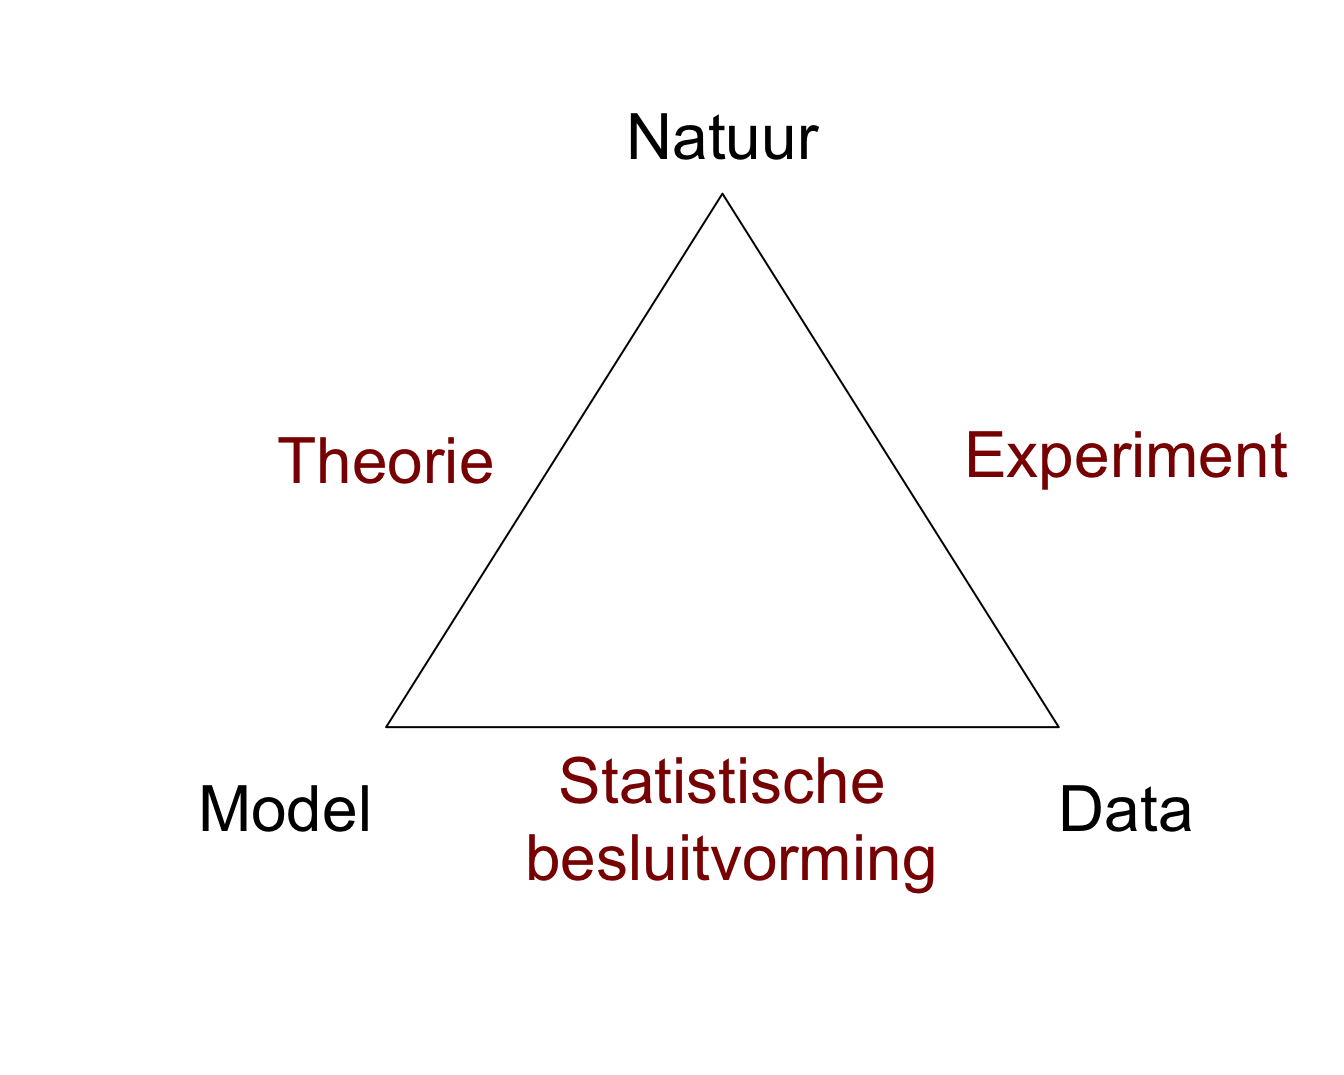
\includegraphics[width=1\linewidth]{Statistiek_2020_2021_files/figure-latex/wetMet-1} 

}

\caption{De Wetenschappelijke Methode en de rol van Statistiek.}\label{fig:wetMet}
\end{figure}

Een andere belangrijke rol van de Statistiek die verder in deze cursus wordt behandeld, is om de \emph{reproduceerbaarheid} van wetenschappelijk onderzoek te waarborgen, binnen zelf gekozen probabiliteitsgrenzen (onzekerheid / zekerheid).

\hypertarget{boutade-met-statistiek-kan-je-alles-bewijzen}{%
\section{Boutade: met statistiek kan je alles bewijzen}\label{boutade-met-statistiek-kan-je-alles-bewijzen}}

In de introductie tonen we aan dat je met statistiek niets kan bewijzen. Statistiek is een hulpmiddel om te leren uit data en om op een reproduceerbare manier conclusies te trekken uit empirisch onderzoek.
Het is eerder zo dat men met foute toepassing van de statistiek alles probeert te bewijzen!

\hypertarget{opzet-van-de-cursus}{%
\section{Opzet van de cursus}\label{opzet-van-de-cursus}}

We leven in een tijd van big data en het is cruciaal om informatie uit cijfers te kunnen extraheren. Statistiek is nu net de wetenschap om te leren uit empirische gegevens.

Statistische geletterdheid is dus een noodzaak om de resultaten uit deze analyses in wetenschappelijke tijdschriften of in de media kritisch te kunnen interpreteren.

Hierbij is het belangrijk om inzicht te verwerven in statistische data analyse enerzijds en om anderzijds deze analyse te interpreteren. We moeten de analyse m.a.w. kunnen koppelen aan de context van het onderzoek: de onderzoeksvraag, de proefopzet en de eigenschappen van de data.
Daarom gaan we alle statistische methodes in de cursus aanbrengen aan de hand van case studies.
We gaan hierbij steeds stilstaan bij

\begin{enumerate}
\def\labelenumi{\arabic{enumi}.}
\item
  de proefopzet en context van de studie (experimenteel ontwerp),
\item
  eigenschappen van de ruwe data (data exploratie), en
\item
  hoe we de resultaten uit de steekproef kunnen veralgemenen naar de populatie toe (statistische besluitvorming).
\item
  Om statistische geletterdheid te verwerven is het ook cruciaal om zelf eenvoudige statistische analyses uit te kunnen voeren zodat je data leert analyseren en te interpreteren. We zullen dus ook in elke case study stilstaan bij hoe we de data analyse uit moeten voeren in statistische software.
\end{enumerate}

In de cursus maken we hiervoor gebruik van
het statistische software pakket R. De cursus en de case studies werden volledig in rmarkdown aangemaakt, dit zijn geavanceerde scripts die toelaten om

\begin{itemize}
\tightlist
\item
  tekst
\item
  formules
\item
  code en
\item
  R output en plots
\end{itemize}

op een efficiënte manier te combineren. Het rmarkdown script kan dan worden gecompileerd naar een webpagina of een pdf document. Op deze manier kan je een data analyse op een volledig reproduceerbare manier documenteren. De scripts van de cursus vormen een goede inspiratiebron om zelf met rmarkdown aan de slag te gaan.

De cursus wordt volledig in online leerpaden verzorgt op het platform Dodona.
Daarbij gaan we hand-on leren statistische programmeren in 2 modules:

\begin{enumerate}
\def\labelenumi{\arabic{enumi}.}
\item
  Module: Introduction to R, waarbij jullie interactief kennis maken met het statistische software pakket en programmeer taal R. Week 1 - Week 3.
\item
  Module: Data exploration and visualisation waarbij jullie de basis principes zullen leren van het maken van goede grafieken die je inzicht zullen geven in de data die wordt gegenereerd in het experiment. Week 4 - 5.
\item
  Module: Statistiek, het hart van deze cursus, waarin jullie inzicht zullen verwerven in de drie belangrijke takken van de statistiek. Week 1-12.

  \begin{itemize}
  \tightlist
  \item
    proefopzet ook wel experimental design genoemd,
  \item
    data exploratie
  \item
    statistische besluitvorming ook wel inferentie genoemd.
  \end{itemize}
\end{enumerate}

Hierbij staat steeds een echte dataset centraal zodat jullie de vertaalslag leren maken van de onderzoeksvraag naar statistisch modellen toe om dan na de data analyse de resultaten opnieuw te interpreteren in termen van de onderzoeksvraag.

We zullen ook telkens alle code delen die nodig is om alle data analyses en visualisaties uit te voeren die worden weergegeven in deze cursus.

In deze inleiding introduceren we drie case studies die het belang van statistiek illustreren.

\begin{enumerate}
\def\labelenumi{\arabic{enumi}.}
\item
  Case study I: Het oksel microbiome. In deze case study doorlopen we alle belangrijke stappen van een experimentele study.
\item
  Case study II: Verschil in lichaamslengte tussen vrouwen en mannen. In deze studie zal je inzicht verwerven in hoe observaties, resultaten en conclusies van een studie onderhevig zijn aan variabiliteit.
\item
  Case study III: Salk vaccin studie voor polio. Deze studie illustreert het belang van een goede controle en introduceert het concept van confounding.
\end{enumerate}

Tijdens de eerste lezing van dit hoofdstuk is het nog niet belangrijk om te focussen op de code. Probeer vooral inzicht te verwerven in het theoretisch raamwerk dat wordt geïntroduceerd. Na week 4 kan het nuttig zijn om de case studies nog eens door te nemen met het oog op hoe je de analyses concreet uit kan voeren.

\hypertarget{case-study-oksel-microbiome}{%
\section{Case study: oksel microbiome}\label{case-study-oksel-microbiome}}

\url{https://www.vrt.be/vrtnws/nl/2018/10/22/gezocht-mensen-met-penetrante-lijfgeur-om-probiotische-deodor/}

Zweten en vooral een zweetgeur is vervelend.
Het zweten op zich is niet de oorzaak van de geur.
Het zijn de microorganismen onder de oksel die het zweet metaboliseren die de geur veroorzaken.
De samenstelling van de gemeenschap van microorganismen onder de oksel is dus bepalend voor het hebben van een zweetgeur.
Deze gemeenschap wordt ook het oksel microbiome genoemd.

Corynebacterium is een bacterië die zweet metaboliseert en hierbij verzadigde vetzuren aanmaakt met een penetrante geur.
Gelukkig zijn er Staphylococcus bacteriën die het zweet ook metaboliseren maar die hierbij geen hinderlijke verzadigde vetzuren produceren.

Het CMet Lab aan de Universiteit Gent doet onderzoek naar microbiële gemeenschappen en stelde een therapie voor om mensen van dit probleem af te helpen.
Die bestaat uit een antibiotica behandeling van de oksel om microbiome af te doden,
gevolgd door een transplantatie van het microbiome van een persoon zonder zweetgeur.

Alvorens dat de therapie breed kan worden ingezet, dient eerst te worden aangetoond in een experiment dat ze werkt.

\hypertarget{experimenteel-design-proefopzet}{%
\subsection{Experimenteel design (proefopzet)}\label{experimenteel-design-proefopzet}}

Een eerste tak van de statistiek focust op experimenteel design.
Idealiter zouden we de therapie evalueren door het uit te testen op de volledige populatie van personen met een zweetgeur.
Dat is echter niet haalbaar omdat het

\begin{enumerate}
\def\labelenumi{\arabic{enumi}.}
\tightlist
\item
  ethisch niet verantwoord is: we weten niet of therapie werkt
\item
  financieel en logistiek onmogelijk is om iedereen te bemonsteren, en omdat
\item
  de populatie waarover we uitspraken wensen te doen bestaat nog niet volledig: ze omvat ook toekomstige personen met een zweetgeur.
\end{enumerate}

Daarom zullen we een steekproef nemen.
Hierbij zullen we een aantal personen uit de populatie selecteren waarop we het experiment uit zullen voeren.

Cruciaal is hierbij dat de steekproef representatief is voor de populatie zodat we de resultaten van het experiment zullen kunnen veralgemenen naar de populatie. We zullen de mensen daarom volledig at random trekken uit de populatie zodat elk subject een zelfde kans heeft om in het experiment te worden opgenomen: randomisatie.
Merk ook op dat het daarom heel belangrijk om de populatie goed te omschrijven voor de start van het experiment: scope van de studie.

In deze studie worden twintig personen met een zweetgeur volledig at random geselecteerd uit de populatie.
We zouden nu elk subject kunnen behandelen.
Maar, dan zijn we niet zeker dat een verschil in het microbiome te wijten is aan de behandeling.

We hebben dus een goeie controle nodig.
We zouden de controle personen niet kunnen behandelen, maar dan kan een verschil in microbiome mogelijks ook te wijten zijn aan de antibiotica behandeling i.p.v. aan de transplantatie.
De onderzoekers opteerden daarom 10 personen een placebo behandeling geven, enkel antibiotica behandeling en 10 personen te behandelen met antibiotica en de transplantatie.

De proefpersonen worden volledig at random toegewezen aan de behandelingsgroep zodat beide groepen vergelijkbaar zijn.

Vervolgens moet er stil worden gestaan bij hoe het microbiome zal worden gemeten?

In de studie maakte men gebruik van een DGGE meting.
Microorganismen hebben een heel variabel stukje ribosomaal RNA, het 16s ribosomaal RNA dat uniek is voor de soort.
Het 16S rRNA van de verschillende microorganismen in het staal wordt dan geamplificeerd en gescheiden op een DGGE gel.
Waarbij een bandenpatroon ontstaat volgens de lengte van het 16s rRNA.

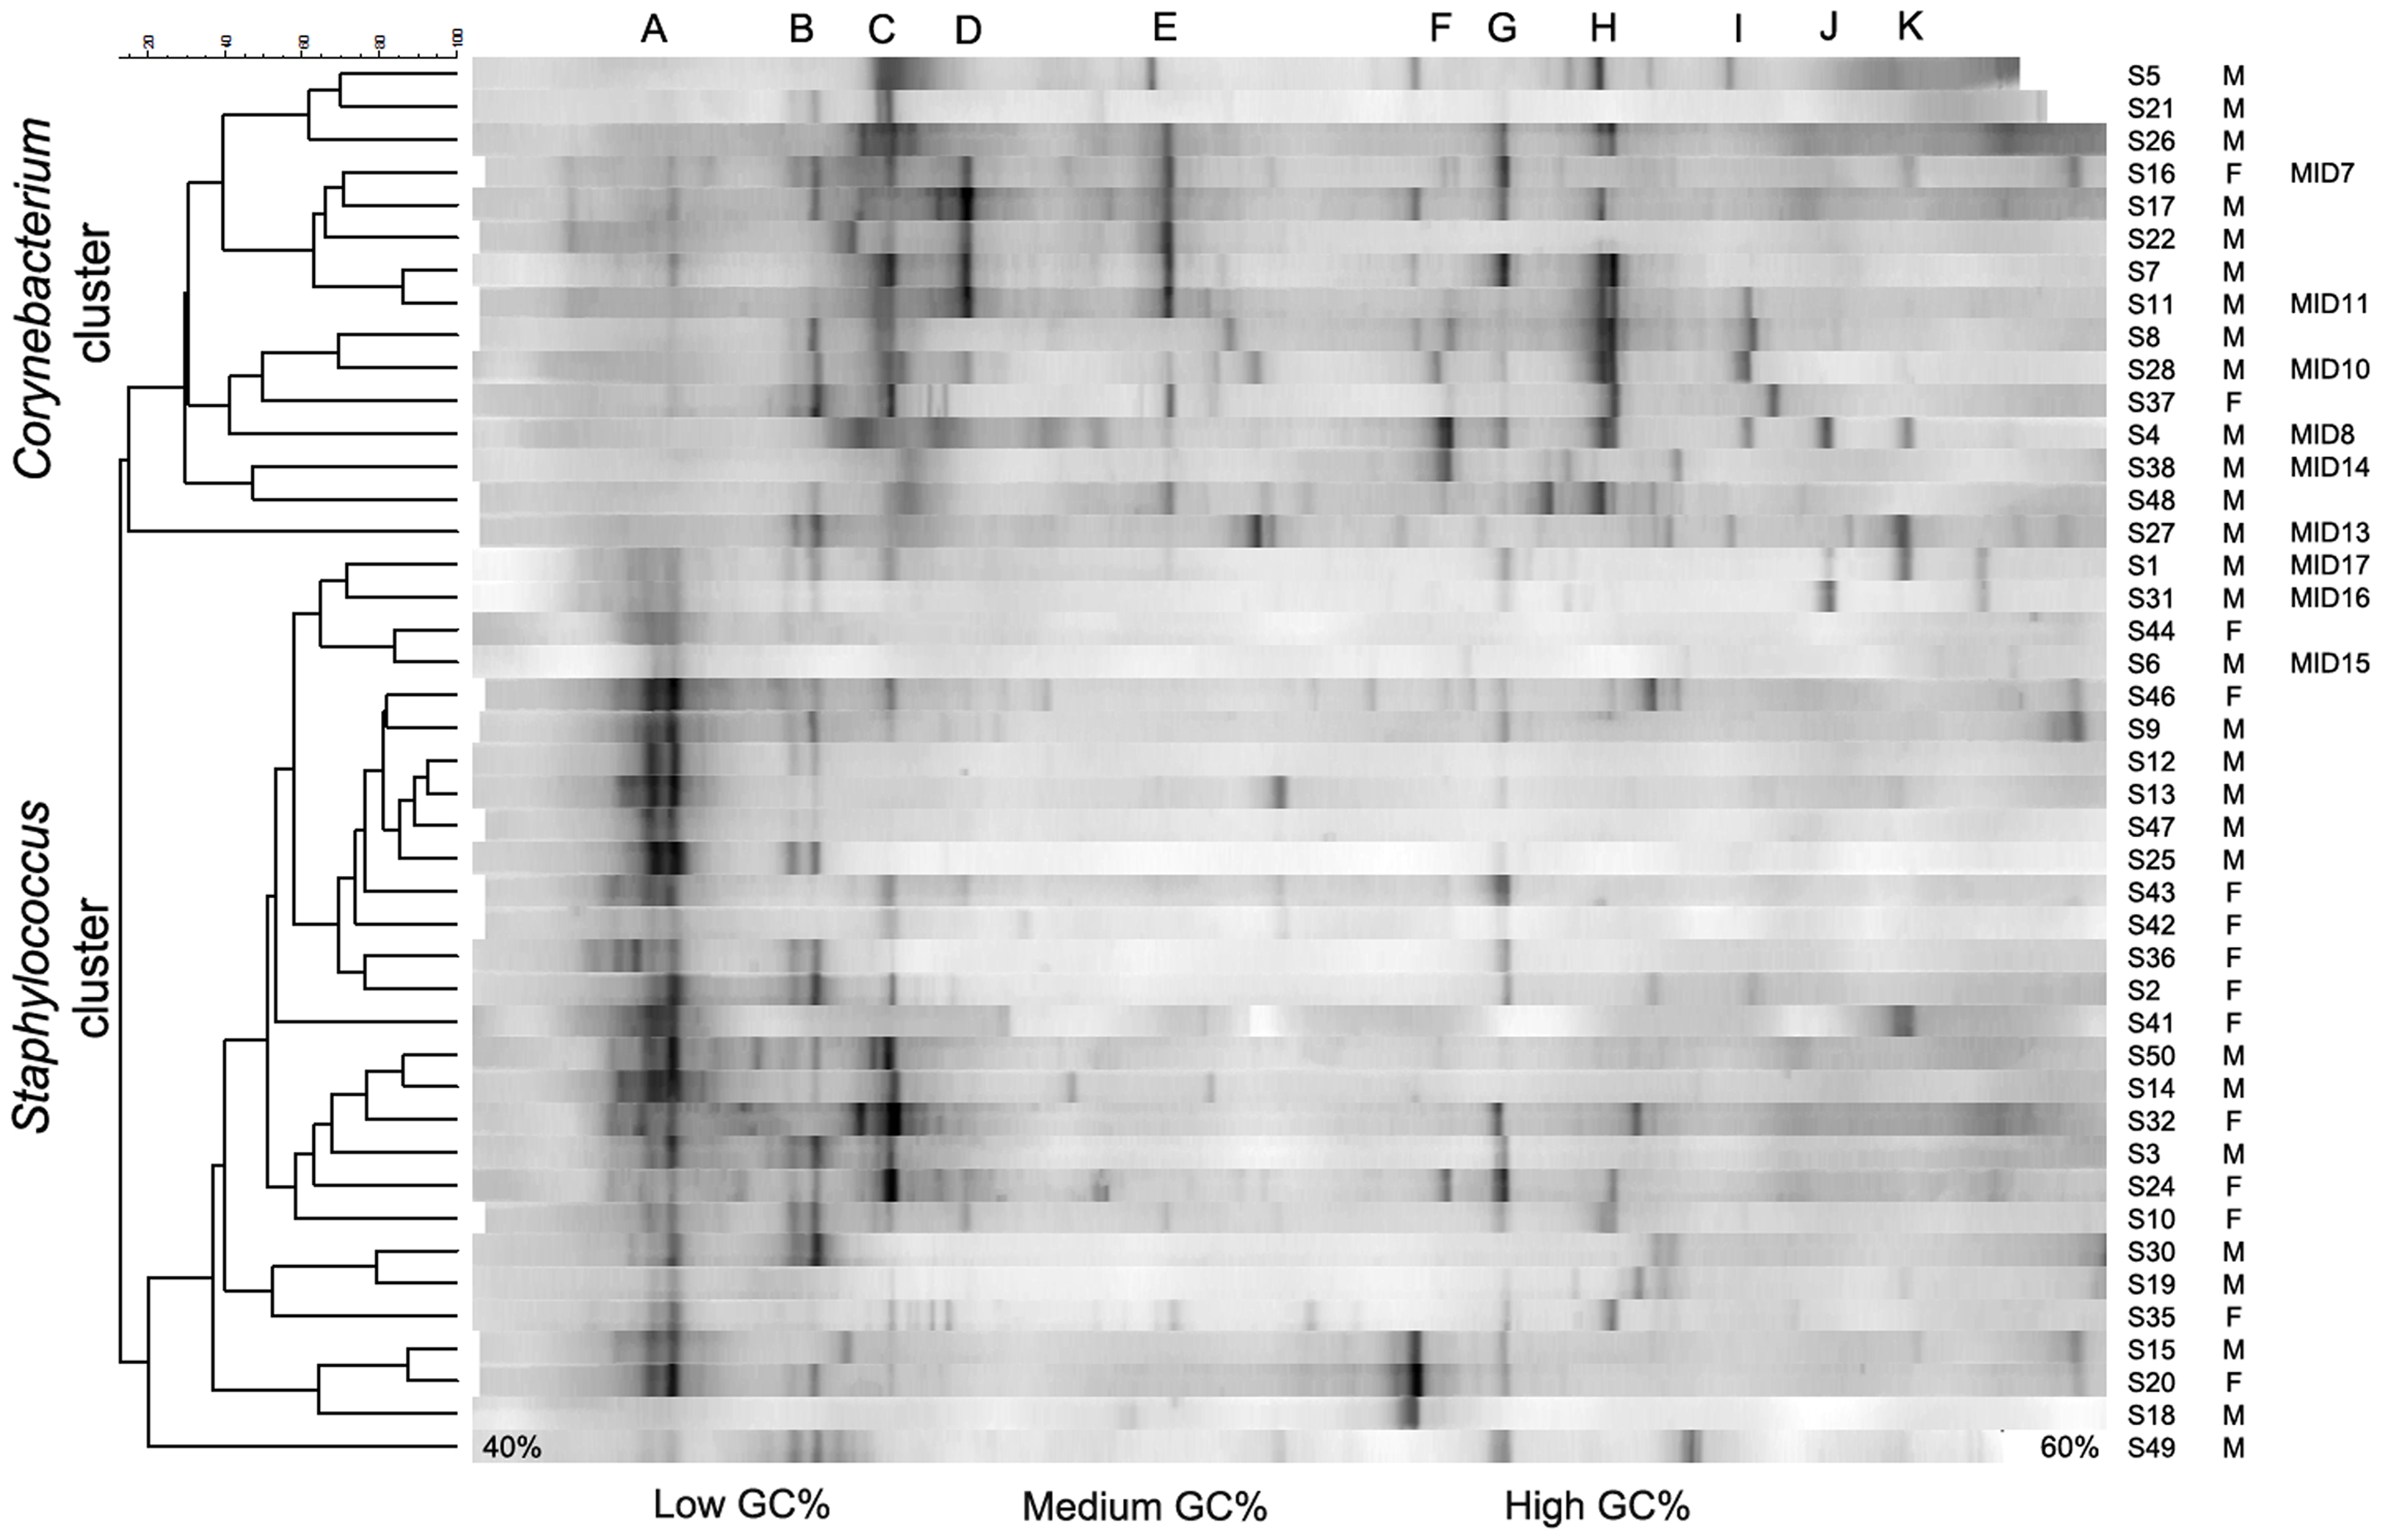
\includegraphics[width=0.7\textwidth,height=\textheight]{../figures/dgge.png}
Foto van een DGGE gel van het oksel microbiome (bron: \url{https://doi.org/10.1371/journal.pone.0070538})

Elke band in de DGGE correspondeert met een bacterie.
Hoe helderder de band hoe meer van de bacterie in het microbiome voorkomt.
Band A staat voor Staphylococcus.
De ratio van de intensiteit van de band en de totale intensiteit in het bandenpatroon kan worden gebruik als een proxy voor de relatieve abundantie.

\emph{Essentiële stap: Vertaal onderzoeksvraag nu naar iets wat we kunnen quantificeren!}

We kunnen dit doen door middel van het gemiddeld verschil in relatieve abundantie in Staphylococcus tussen de transplantatie en placebo groep.

Het experiment kan nu worden uitgevoerd.

\hypertarget{data-exploratie-en-beschrijvende-statistiek}{%
\subsection{Data exploratie en beschrijvende statistiek}\label{data-exploratie-en-beschrijvende-statistiek}}

Data exploratie is heel belangrijk om inzicht te krijgen in de data en is een essentiële eerste stap om te leren uit data.
Het wordt vaak ondergewaardeerd of over het hoofd gezien.

Data in deze cursus wordt verwerkt via het statistisch software pakket R.
Vooraleer we met de data exploratie van start kunnen gaan moeten we de data eerst importeren in R.

We geven duidelijk aan welke delen van de tekst over het Code gaan en welke over de interpretatie. Probeer initiëel te focussen op de interpretatie. Het Code zal je immers gedurende de eerste weken oppikken. Daarom hebben we ook gekozen om aparte clips te maken m.b.t interpretatie en Code. Zodat de manier hoe je de data analyse dient uit te voeren het begrip initiëel niet in de weg staan.

\hypertarget{importeer-de-data}{%
\subsubsection{Importeer de data}\label{importeer-de-data}}

\emph{Code} Tijdens de data exploratie gaan we voor de data manipulaties veelal gebruik maken van functies uit het \texttt{tidyverse} package.
Dat kan worden geladen door het commando
\texttt{library(tidyverse)}.

Via het commando \texttt{read\_lines} kunnen we enkele regels van een data bestand inlezen om de structuur van het data bestand te weten te komen.

\begin{Shaded}
\begin{Highlighting}[]
\KeywordTok{library}\NormalTok{(tidyverse)}
\KeywordTok{read\_lines}\NormalTok{(}\StringTok{"https://raw.githubusercontent.com/statOmics/sbc20/master/data/armpit.csv"}\NormalTok{)}
\end{Highlighting}
\end{Shaded}

\begin{verbatim}
##  [1] "trt,rel"                       "placebo,54.99207606973059"    
##  [3] "placebo,31.84466019417476"     "placebo,41.09947643979057"    
##  [5] "placebo,59.52063914780293"     "placebo,63.573407202216075"   
##  [7] "placebo,41.48648648648649"     "placebo,30.44041450777202"    
##  [9] "placebo,42.95676429567643"     "placebo,41.7391304347826"     
## [11] "placebo,33.896515311510036"    "transplant,57.218124341412015"
## [13] "transplant,72.50900360144058"  "transplant,61.89258312020461" 
## [15] "transplant,56.690140845070424" "transplant,76"                
## [17] "transplant,71.7357910906298"   "transplant,57.757296466973884"
## [19] "transplant,65.1219512195122"   "transplant,67.53424657534246" 
## [21] "transplant,77.55359394703657"
\end{verbatim}

We observeren de volgende structuur:

\begin{itemize}
\tightlist
\item
  Gegevens in het bestand zijn door comma's gescheiden.
\item
  Elke rij bevat de gegevens voor 1 proefpersoon
\item
  Verschillende variabelen worden gemeten per persoon en zijn van elkaar gescheiden door een comma. Het bestand is in csv formaat: ``comma separated values''.
\item
  We kunnen bestanden met dit formaat inlezen R via het commando \texttt{read\_csv}.
\item
  We slaan de data op in R in het object met naam ap. Hiervoor gebruiken we de \texttt{\textless{}-} operator.
\item
  We geven de data tabel terug door het object aan te roepen door zijn naam te typen.
\end{itemize}

\begin{Shaded}
\begin{Highlighting}[]
\NormalTok{ap \textless{}{-}}\StringTok{ }\KeywordTok{read\_csv}\NormalTok{(}\StringTok{"https://raw.githubusercontent.com/statOmics/sbc20/master/data/armpit.csv"}\NormalTok{)}
\NormalTok{ap}
\end{Highlighting}
\end{Shaded}

\begin{verbatim}
## # A tibble: 20 x 2
##    trt          rel
##    <chr>      <dbl>
##  1 placebo     55.0
##  2 placebo     31.8
##  3 placebo     41.1
##  4 placebo     59.5
##  5 placebo     63.6
##  6 placebo     41.5
##  7 placebo     30.4
##  8 placebo     43.0
##  9 placebo     41.7
## 10 placebo     33.9
## 11 transplant  57.2
## 12 transplant  72.5
## 13 transplant  61.9
## 14 transplant  56.7
## 15 transplant  76  
## 16 transplant  71.7
## 17 transplant  57.8
## 18 transplant  65.1
## 19 transplant  67.5
## 20 transplant  77.6
\end{verbatim}

Als we data matrix observeren zien we de volgende structuur:
proefpersonen in de rijen waarvoor we twee karateristieken (variabelen) hebben bijgehouden per subject:
behandeling (trt) en relatieve abundantie (rel).
Deze data structuur wordt \texttt{tidy\ data} genoemd.

Weinig mensen kunnen a.d.h.v. het bekijken van de data matrix structuur of patronen zien in de data. Daarom zullen we de data moeten verwerken en visualiseren.

\hypertarget{beschrijvende-statistiek}{%
\subsubsection{Beschrijvende statistiek}\label{beschrijvende-statistiek}}

In artikels en de media worden resultaten uit een steekproef vaak gerapporteerd a.d.h.v. gemiddelde en de standaardafwijking.

\emph{Code}

\begin{itemize}
\tightlist
\item
  We vatten de data eerst samen. We berekenen het gemiddelde en de standaard deviatie (een maat voor de spreiding, zie volgende hoofdstukken).
  We slaan het resultaat hiervan op in het object apRelSum via \texttt{apRelSum\ \textless{}-}.
\end{itemize}

\begin{enumerate}
\def\labelenumi{\arabic{enumi}.}
\item
  We pipen (via \texttt{\%\textgreater{}\%}) het \texttt{ap} dataframe naar de \texttt{group\_by} functie om de data te groeperen per treatment trt: \texttt{group\_by(trt)}.
\item
  We pipen het resultaat naar de \texttt{summarize\_at} function om de ``rel'' variable samen te vatten en berekenen hierbij het gemiddelde en standaardafwijking. Omdat we de data eerst hebben gegroepeerd zullen we het gemiddelde en de standaard deviatie berekenen per groep.
\end{enumerate}

\begin{Shaded}
\begin{Highlighting}[]
\NormalTok{apRelSum \textless{}{-}}\StringTok{ }\NormalTok{ap }\OperatorTok{\%\textgreater{}\%}\StringTok{ }\KeywordTok{group\_by}\NormalTok{(trt) }\OperatorTok{\%\textgreater{}\%}\StringTok{ }\KeywordTok{summarize\_at}\NormalTok{(}\StringTok{"rel"}\NormalTok{, }
    \KeywordTok{list}\NormalTok{(}\DataTypeTok{mean =}\NormalTok{ mean, }\DataTypeTok{sd =}\NormalTok{ sd))}
\end{Highlighting}
\end{Shaded}

We tonen vervolgens het resultaat door het object apRelSum aan te roepen

\begin{Shaded}
\begin{Highlighting}[]
\NormalTok{apRelSum}
\end{Highlighting}
\end{Shaded}

\begin{verbatim}
## # A tibble: 2 x 3
##   trt         mean    sd
##   <chr>      <dbl> <dbl>
## 1 placebo     44.2 11.5 
## 2 transplant  66.4  7.88
\end{verbatim}

We kunnen ook een tabel in de webpagina of het pdf bestand integreren via het commando kable van het knitr pakket:

\begin{Shaded}
\begin{Highlighting}[]
\NormalTok{knitr}\OperatorTok{::}\KeywordTok{kable}\NormalTok{(apRelSum, }\StringTok{"html"}\NormalTok{)}
\end{Highlighting}
\end{Shaded}

trt

mean

sd

placebo

44.15496

11.543251

transplant

66.40127

7.880175

\emph{Interpretatie}

Het effect van de behandeling in de steekproef kan worden gekwantificeerd door de gemiddelde relatieve abundantie te vergelijken in elke steekproef. We observeren dat de gemiddelde relatieve abundantie in de steekproef gemiddeld 22.2\% hoger is in de transplantatie dan in de placebo groep.

We quantificeren ook de variabiliteit of de spreiding van de gegevens rond het gemiddelde aan de hand van de standaardafwijking.

Het gemiddelde en de standaardafwijking wordt ook vaak grafisch weergegeven in een barplot.

\emph{Code}
We maken in deze cursus gebruik van het pakket \texttt{ggplot2} om grafieken te maken.\\
Met de ggplot2 bibliotheek kunnen we gemakkelijk grafieken opbouwen in lagen (layers).
Hierdoor leest de code veel makkelijker.
In uitgebreide introductie tot ggplot vinden je in de Dodona module \href{https://dodona.ugent.be/nl/courses/345/}{R data exploration and visualisation}.

Bar plots worden heel veel gebruikt in artikels om resultaten weer te geven.

\begin{enumerate}
\def\labelenumi{\arabic{enumi}.}
\item
  We pipen de samengevatte data naar de functie \texttt{ggplot}. Dat is de basis van elke ggplot. We selecteren de variabele met de behandeling trt als x variabele en de variabele met naam mean als y-variabele voor de plot.
  We doen dit steeds via de aestetics \texttt{aes} functie. \texttt{aes(x=trt,y=mean)}
\item
  We maken een barplot door een laag toe te voegen via de \texttt{geom\_bar} function. De statistiek is \texttt{stat="identity"} omdat de hoogte van de bar gelijk is aan de waarde voor y (hier het gemiddelde voor de relatieve abundantie).
\item
  We voegen foutenvlaggen toe om de onzekerheid op het gemiddelde weer te geven. We doen dit via de \texttt{geom\_errorbar} functie en specifiëren het minimum en maximum van de error bar. Het \texttt{width} argument wordt gebruikt om de breedte van de error bar smaller te maken dat deze van de bar.
\end{enumerate}

\begin{Shaded}
\begin{Highlighting}[]
\NormalTok{apRelSum }\OperatorTok{\%\textgreater{}\%}\StringTok{ }\KeywordTok{ggplot}\NormalTok{(}\KeywordTok{aes}\NormalTok{(}\DataTypeTok{x =}\NormalTok{ trt, }\DataTypeTok{y =}\NormalTok{ mean)) }\OperatorTok{+}\StringTok{ }\KeywordTok{geom\_bar}\NormalTok{(}\DataTypeTok{stat =} \StringTok{"identity"}\NormalTok{) }\OperatorTok{+}\StringTok{ }
\StringTok{    }\KeywordTok{geom\_errorbar}\NormalTok{(}\KeywordTok{aes}\NormalTok{(}\DataTypeTok{ymin =}\NormalTok{ mean }\OperatorTok{{-}}\StringTok{ }\NormalTok{sd, }\DataTypeTok{ymax =}\NormalTok{ mean }\OperatorTok{+}\StringTok{ }
\StringTok{        }\NormalTok{sd), }\DataTypeTok{width =} \FloatTok{0.2}\NormalTok{)}
\end{Highlighting}
\end{Shaded}

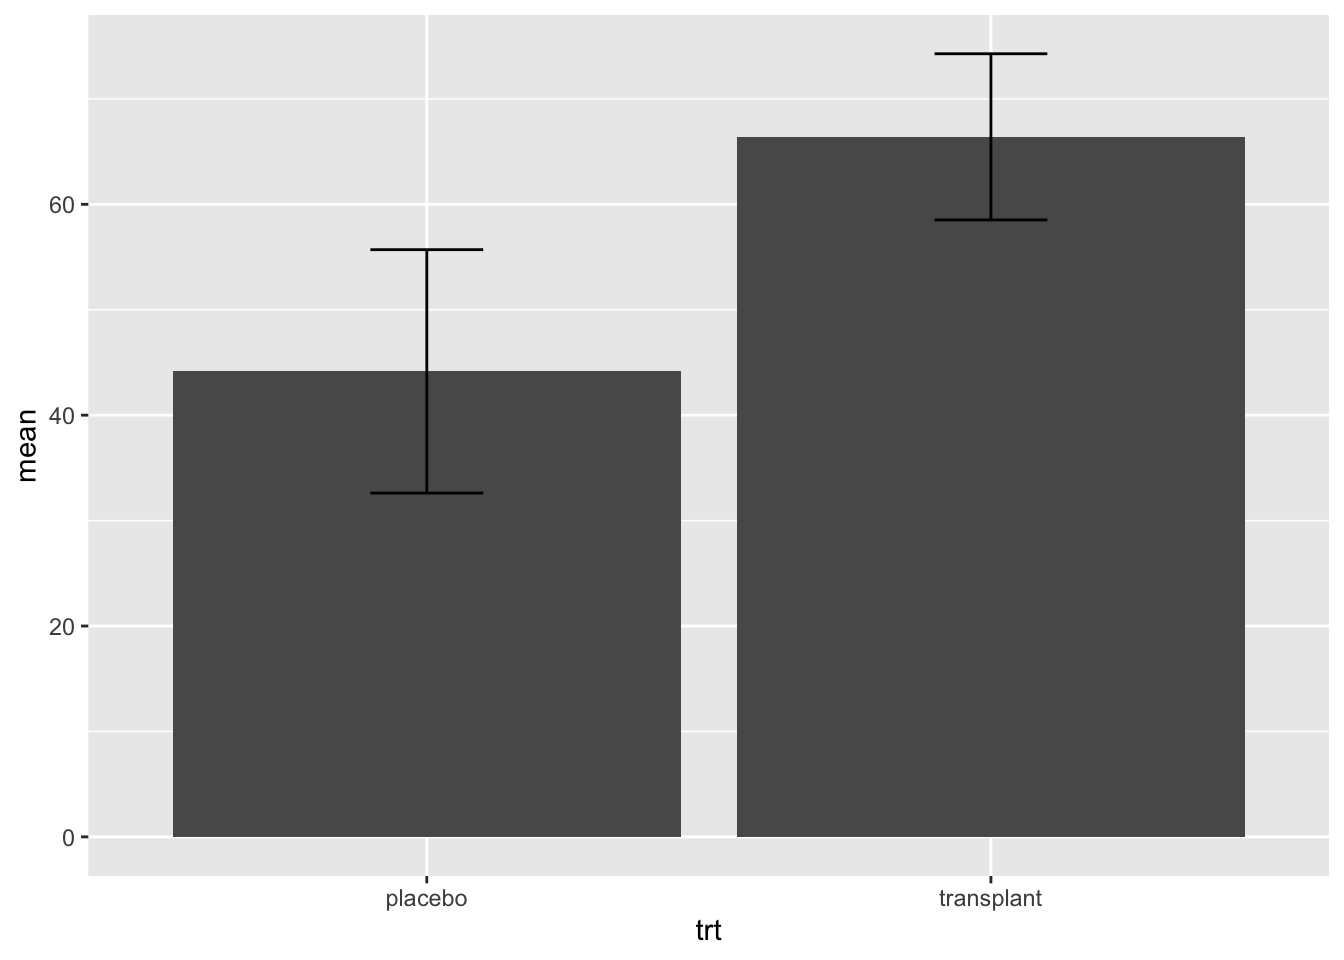
\includegraphics{Statistiek_2020_2021_files/figure-latex/unnamed-chunk-7-1.pdf}

\emph{Interpretatie}

Is deze plot informatief? Nee!

We zien enkel een ``two-number summary'': het gemiddelde en de standaarddeviatie. We weten niet of deze wel een goeie samenvattende maat zijn voor de data. Bovendien wordt heel wat ruimte in de plot benut die niet informatief is: er zijn bijvoorbeeld geen observaties met relatieve abundanties van 0\%.

Om de data van verschillende groepen makkelijk te kunnen vergelijken in een grafiek die meer informatief is dan de bar plot ontwikkelde Tukey de boxplot. Dit is een ``five-number summary'' het bereik van de data (minimum en maximum) samen met het 25, 50 (mediaan), and 75 percentiel. Deze percentielen zijn de waarden waarvoor respectievelijk 25\%, 50\% en 75\% van de data in de steekproef kleiner zijn. Tukey raadde aan om het bereik van de data te berekenen zonder rekening te houden met outliers (extreme observaties). De outliers worden afzonderlijk als data punten toegevoegd aan de plot. In het hoofdstuk 4: Data Exploratie leggen we uit wat outliers precies zijn.

\emph{Code}
We maken nu een boxplot voor de ap data

\begin{enumerate}
\def\labelenumi{\arabic{enumi}.}
\tightlist
\item
  We pipen het \texttt{ap} data object naar \texttt{ggplot}
\item
  We selecteren de data voor de plot via \texttt{ggplot(aes(x=trt,y=rel))}
\item
  We voegen een laag toe voor de boxplot dmv de functie \texttt{geom\_boxplot()}
\end{enumerate}

\begin{Shaded}
\begin{Highlighting}[]
\NormalTok{ap }\OperatorTok{\%\textgreater{}\%}\StringTok{ }\KeywordTok{ggplot}\NormalTok{(}\KeywordTok{aes}\NormalTok{(}\DataTypeTok{x =}\NormalTok{ trt, }\DataTypeTok{y =}\NormalTok{ rel)) }\OperatorTok{+}\StringTok{ }\KeywordTok{geom\_boxplot}\NormalTok{()}
\end{Highlighting}
\end{Shaded}

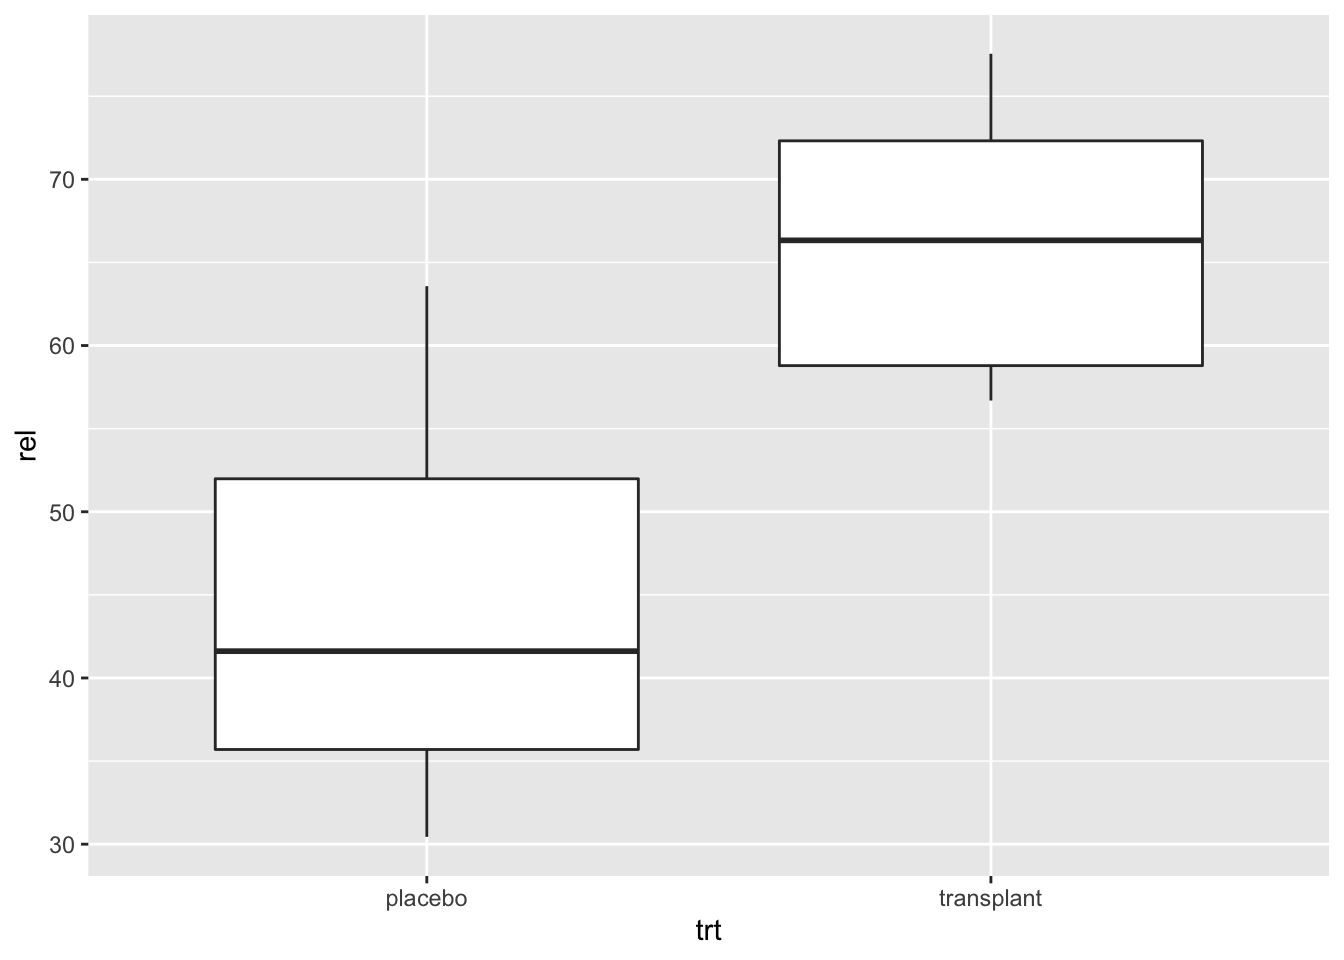
\includegraphics{Statistiek_2020_2021_files/figure-latex/unnamed-chunk-8-1.pdf}

\emph{Interpretatie}: De boxplot geeft ons al veel meer informatie dan de barplot. Het bereik van de data wordt weergegeven door de wiskers (eindpunten van de verticale lijnen in het midden van de boxplot). De box in de boxplot geeft het 25\%, 50\% en 75\% percentiel weer. (Merk op dat er geen outliers zijn. Er worden geen individuele punten weergegeven in de plot)

We observeren dat boxplot voor de transplantie groep hoger ligt dan voor de placebo groep. Wat aangeeft dat de relatieve abundanties van Staphylococcus vaak hoger liggen voor personen in de steekproef die zijn toegewezen aan de transplantatie groep dan voor personen die zijn toegewezen aan placebo groep. Dit is een indicatie dat de behandeling werkt.

Verder weten we dat er maar 10 observaties zijn in elke groep. Dat laat toe om de ruwe gegevens aan de plot toe te voegen zonder dat de plot te druk wordt.

\emph{Code}

\begin{itemize}
\tightlist
\item
  Merk op dat we het argument \texttt{outlier.shape} op NA (not available) zetten \texttt{outlier.shape=NA} in the \texttt{geom\_boxplot} functie. Dat doen we standaard als we de ruwe data toevoegen aan de boxplots: anders zullen outliers immers twee keer worden weergegeven (eerst via de boxplot laag en daarna door de laag met alle ruwe data toevoegen aan de plot).
\item
  We geven de ruwe data weer via de \texttt{geom\_point(position="jitter")} functie. We gebruiken hierbij het argument position=`jitter' zodat we wat random ruis toevoegen aan de x-cordinaat zodat de gegevens elkaar niet overlappen.
\end{itemize}

\begin{Shaded}
\begin{Highlighting}[]
\NormalTok{ap }\OperatorTok{\%\textgreater{}\%}\StringTok{ }\KeywordTok{ggplot}\NormalTok{(}\KeywordTok{aes}\NormalTok{(}\DataTypeTok{x =}\NormalTok{ trt, }\DataTypeTok{y =}\NormalTok{ rel)) }\OperatorTok{+}\StringTok{ }\KeywordTok{geom\_boxplot}\NormalTok{(}\DataTypeTok{outlier.shape =} \OtherTok{NA}\NormalTok{) }\OperatorTok{+}\StringTok{ }
\StringTok{    }\KeywordTok{geom\_point}\NormalTok{(}\DataTypeTok{position =} \StringTok{"jitter"}\NormalTok{)}
\end{Highlighting}
\end{Shaded}

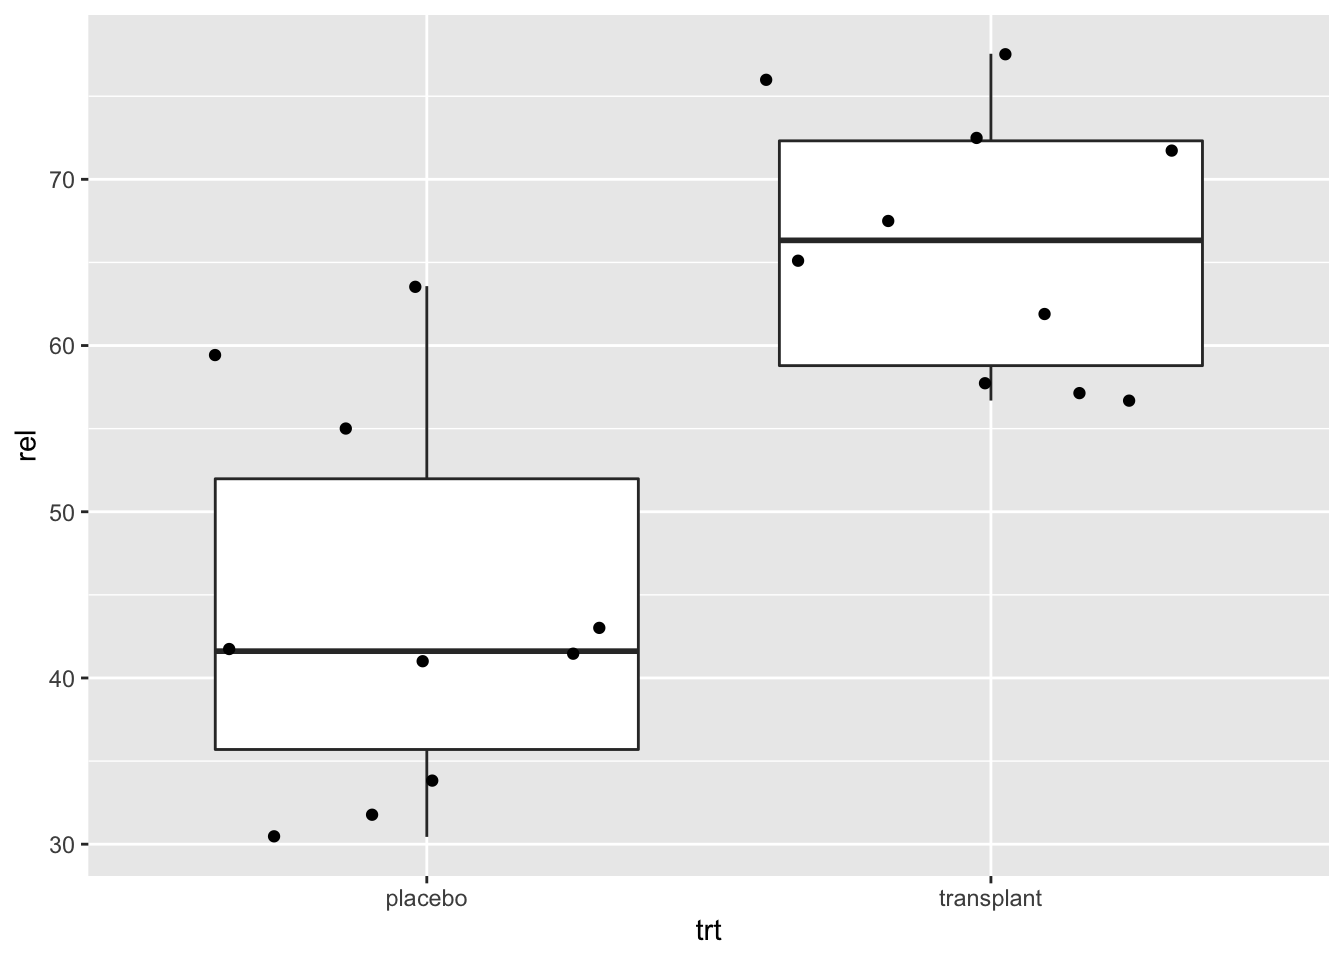
\includegraphics{Statistiek_2020_2021_files/figure-latex/unnamed-chunk-9-1.pdf}

Dit is een informatieve plot!
Het toont de data zo ruw mogelijk weer. De plot is toch nog goed leesbaar en toont duidelijk aan dat de relatieve abundanties bij bijna alle proefpersonen in de transplantatie groep hoger is dan deze voor de placebo groep.

\hypertarget{statistische-besluitvorming}{%
\subsection{Statistische Besluitvorming}\label{statistische-besluitvorming}}

We zagen duidelijk een effect van de transplantatie op de relatieve abundantie van Staphylococcus.
We vragen ons nu af of het effect groot genoeg om te kunnen concluderen dat de behandeling werkt?

Hoe kunnen we met andere woorden de conclusies uit de steekproef veralgemenen naar de populatie toe? \emph{inductie}.
Op basis van de steekproef kunnen we het effect, gemiddeld verschil in relatieve abundantie tussen beide behandelingsgroepen, schatten in de populatie.
De prijs die we hiervoor betalen is onzekerheid!
Omdat we niet alle personen in de populatie hebben kunnen testen zullen we echter nooit absoluut zeker kunnen zijn over onze conclusies.

Om de conclusies uit de steekproef te veralgemenen naar de populatie maken we gebruik van een derde tak van de statistiek:
Statistische besluitvorming.

\begin{itemize}
\item
  Met data kunnen we niet bewijzen dat een behandeling werkt.
\item
  Falsificatie principe van Popper: Data kunnen enkel een hypothese of een theorie ontkrachten.
\item
  Met statistiek kunnen we dus niet aantonen dat de behandeling werkt.
\item
  Statistiek zal ons wel toelaten om het omgekeerde te falsifiëren: als we veronderstellen dat er geen effect van de behandeling, spreekt de data in de steekproef dit tegen?
\end{itemize}

Met statistiek kunnen we berekenen hoe waarschijnlijk het is om in een random steekproef (nieuw experiment) een verschil in gemiddelde relatieve abundantie te zien tussen transplantatie (\(\bar X_\text{transplant}\)) en placebo groep (\(\bar X_\text{placebo}\)) dat minstens 22.2\% bedraagt als de behandeling geen effect zou hebben.

\[p=P( \vert \bar X_\text{transplant}-\bar X_\text{placebo}\vert \vert \geq 22.2\% \vert \text{geen effect van de behandeling})\]

\begin{itemize}
\item
  Die kans wordt een p-waarde genoemd.
\item
  Als p heel klein is, dan is het heel onwaarschijnlijk om een dergelijk effect door toeval te observeren in een steekproef als er in werkelijkheid geen effect is van de behandeling.
\end{itemize}

Om de kans p te berekenen is het nodig om de data te modelleren met een statistisch model. Hiervoor zullen we bepaalde aannames moeten doen. In hoofdstuk 5 zien we dat we dit kunnen doen d.m.v. de \texttt{t.test} functie.

\begin{Shaded}
\begin{Highlighting}[]
\KeywordTok{t.test}\NormalTok{(rel }\OperatorTok{\textasciitilde{}}\StringTok{ }\NormalTok{trt, }\DataTypeTok{data =}\NormalTok{ ap)}
\end{Highlighting}
\end{Shaded}

\begin{verbatim}
## 
## 	Welch Two Sample t-test
## 
## data:  rel by trt
## t = -5.0334, df = 15.892, p-value = 0.0001249
## alternative hypothesis: true difference in means is not equal to 0
## 95 percent confidence interval:
##  -31.62100 -12.87163
## sample estimates:
##    mean in group placebo mean in group transplant 
##                 44.15496                 66.40127
\end{verbatim}

Als er in werkelijkheid geen effect is van de behandeling en als de model aannames correct zijn dan verwachten we in minder dan 2 op 10000 random steekproeven een verschil van minstens 22.2\% in de relatieve abundantie tussen beide behandelingsgroepen.
Deze kans is heel klein. Het is dus heel onwaarschijnlijk om dergelijk verschil in relatieve abundantie te observeren in een random steekproef als er geen effect van de behandeling zou zijn.

We kunnen daarom de hypothese dat er geen effect is van de behandeling verwerpen en concluderen:

Er is een statistisch significant verschil in gemiddelde relatieve abundantie van Staphylococcus in het okselmicrobiome van personen met een zweetgeur die worden behandeld met de transplantie en personen die behandeld worden met de placebo behandeling.
Gemiddeld is de relatieve abundantie van Staphylococcus in het microbiome van personen met een zweetgeur is 22.2\% hoger na microbiome transplantie dan na de placebo behandeling.

\hypertarget{mogelijke-fouten}{%
\subsubsection{Mogelijke fouten}\label{mogelijke-fouten}}

Merk op dat een experiment onderhevig is aan random variabiliteit. Als we het experiment opnieuw uit zouden voeren zullen we andere proefpersonen in de steekproef opnemen. Bijgevolg zullen we ook andere relatieve abundanties meten.

\begin{itemize}
\item
  Daardoor zijn ook onze conclusies onderhevig aan random variabiliteit.
\item
  Zelfs al zou er in werkelijkheid geen effect zijn van de behandeling dan kunnen we in een random steekproef met 10 mensen in de placebo en 10 mensen in de behandelingsgroep toch ook een verschil in relatieve abundantie observeren die minsten 22.2\% is. Dat kunnen we in 1 op de 10000 experimenten verwachten.
\end{itemize}

In dergelijke steekproef zal men ten onrechte besluiten dat er bewijs is dat de transplantie behandeling werkt.

\begin{itemize}
\item
  Intuïtief voelen we aan dat we dus niet met absolute zekerheid uitspraken kunnen doen over populatiekarakteristieken op basis van een eindige steekproef.
\item
  Typisch zullen we de p-waarde vergelijken met 5\% vooraleer we beslissen dat een behandeling werkt. We zullen de kans op het maken van foute conclusies dus controleren op 5\%.
\end{itemize}

In de volgende case studie zullen we bestuderen hoe de metingen, de resultaten en de conclusies kunnen variëren van steekproef tot steekproef.

\hypertarget{case-study-ii-verschil-in-lengte-tussen-vrouwen-en-mannen}{%
\section{Case Study II: Verschil in lengte tussen vrouwen en mannen}\label{case-study-ii-verschil-in-lengte-tussen-vrouwen-en-mannen}}

Om resultaten van een steekproef te kunnen veralgemenen naar de populatie toe trekken we subjecten at random uit de populatie.

Randomisatie is sterk gerelateerd met het concept van de populatie en scope van de studie.
De scope van de studie moet goed worden omschreven voor de start van het experiment. Het is immers de populatie naar waar we de resultaten uit de steekproef kunnen veralgemenen.

We nemen daarom een random steekproef uit de populatie:

\begin{itemize}
\item
  alle subjecten van de populatie hebben dus evenveel kans om in de steekproef te worden opgenomen.
\item
  de selectie van een subject is onafhankelijk van andere subjecten in de steekproef.
\end{itemize}

De steekproef is dan representatief voor de populatie, maar is nog steeds random.

Om te begrijpen dat een steekproef random is zouden we hetzelfde experiment veel keer moeten kunnen herhalen (\texttt{repeated\ sampling}). Dan zouden we inzicht kunnen krijgen hoe de gegevens veranderen van steekproef tot steekproef.

Om dit te illustreren zullen we gebruik maken van de National Health And Nutrition Examination Study (NHANES) studie. Uit die studie kunnen we herhaaldelijk kleine steekproeven trekken om te begrijpen hoe de gegevens en statistieken veranderen van steekproef tot steekproef. Of om met andere woorden na te gaan wat de variabiliteit is tussen steekproeven.

De National Health And Nutrition Examination Study (NHANES) studie:

\begin{itemize}
\item
  Sinds 1960 worden elk jaar mensen van alle leeftijden geïnterviewd bij hen thuis.
\item
  Er maakt ook een gezondheidsonderzoek deel uit van de study die in een mobiel onderzoekscentrum wordt afgenomen.
\item
  We zullen deze grote studie gebruiken om at random personen te selecteren van de Amerikaanse populatie.
\item
  Dat zal inzicht geven in hoe de gegevens en resultaten van een analyse zullen variëren van steekproef tot steekproef.
\end{itemize}

De data van deze studie is terug te vinden in het R pakket \texttt{NHANES}. Met de functie \texttt{head} kunnen we de eerste 6 rijen van de dataset bekijken.

\begin{Shaded}
\begin{Highlighting}[]
\KeywordTok{library}\NormalTok{(NHANES)}
\KeywordTok{head}\NormalTok{(NHANES)}
\end{Highlighting}
\end{Shaded}

\begin{verbatim}
## # A tibble: 6 x 76
##      ID SurveyYr Gender   Age AgeDecade AgeMonths Race1 Race3 Education
##   <int> <fct>    <fct>  <int> <fct>         <int> <fct> <fct> <fct>    
## 1 51624 2009_10  male      34 " 30-39"        409 White <NA>  High Sch~
## 2 51624 2009_10  male      34 " 30-39"        409 White <NA>  High Sch~
## 3 51624 2009_10  male      34 " 30-39"        409 White <NA>  High Sch~
## 4 51625 2009_10  male       4 " 0-9"           49 Other <NA>  <NA>     
## 5 51630 2009_10  female    49 " 40-49"        596 White <NA>  Some Col~
## 6 51638 2009_10  male       9 " 0-9"          115 White <NA>  <NA>     
## # ... with 67 more variables: MaritalStatus <fct>, HHIncome <fct>,
## #   HHIncomeMid <int>, Poverty <dbl>, HomeRooms <int>, HomeOwn <fct>,
## #   Work <fct>, Weight <dbl>, Length <dbl>, HeadCirc <dbl>, Height <dbl>,
## #   BMI <dbl>, BMICatUnder20yrs <fct>, BMI_WHO <fct>, Pulse <int>,
## #   BPSysAve <int>, BPDiaAve <int>, BPSys1 <int>, BPDia1 <int>,
## #   BPSys2 <int>, BPDia2 <int>, BPSys3 <int>, BPDia3 <int>,
## #   Testosterone <dbl>, DirectChol <dbl>, TotChol <dbl>, UrineVol1 <int>,
## #   UrineFlow1 <dbl>, UrineVol2 <int>, UrineFlow2 <dbl>, Diabetes <fct>,
## #   DiabetesAge <int>, HealthGen <fct>, DaysPhysHlthBad <int>,
## #   DaysMentHlthBad <int>, LittleInterest <fct>, Depressed <fct>,
## #   nPregnancies <int>, nBabies <int>, Age1stBaby <int>,
## #   SleepHrsNight <int>, SleepTrouble <fct>, PhysActive <fct>,
## #   PhysActiveDays <int>, TVHrsDay <fct>, CompHrsDay <fct>,
## #   TVHrsDayChild <int>, CompHrsDayChild <int>, Alcohol12PlusYr <fct>,
## #   AlcoholDay <int>, AlcoholYear <int>, SmokeNow <fct>, Smoke100 <fct>,
## #   Smoke100n <fct>, SmokeAge <int>, Marijuana <fct>, AgeFirstMarij <int>,
## #   RegularMarij <fct>, AgeRegMarij <int>, HardDrugs <fct>, SexEver <fct>,
## #   SexAge <int>, SexNumPartnLife <int>, SexNumPartYear <int>,
## #   SameSex <fct>, SexOrientation <fct>, PregnantNow <fct>
\end{verbatim}

We focussen in dit voorbeeld op het verschil in lengte tussen volwassen vrouwen en mannen in de Amerikaanse populatie.

Onderzoeksvraag: hoe verschilt de lengte van volwassen mannen en vrouwen.

We exploreren hiervoor eerst de lengte data in de NHANES studie. Omdat we heel veel gegevens hebben, maken we gebruik van histogrammen om inzicht te krijgen in de verdeling van de data.

\emph{Code}
1. We pipen de dataset naar de function \texttt{filter} om de data te filteren volgens leeftijd. We verwijderen eveneens gegevens waarvoor de lengte metingen ontbreken. Voor deze gevens werd de data ingegeven met de code NA (Not Available)
2. We plotten de lengte metingen.
- We selecteren de data met het commando \texttt{ggplot(aes(x=lengte))}
- We voegen een histogram toe met het commando \texttt{geom\_histogram()}
- We maken twee vertikale panels met het commando \texttt{facet\_grid(Gender\textasciitilde{}.)}. Een panel per geslacht.
- We veranderen het label van de x-as met de \texttt{xlab} functie.

\begin{Shaded}
\begin{Highlighting}[]
\NormalTok{NHANES }\OperatorTok{\%\textgreater{}\%}\StringTok{ }\KeywordTok{filter}\NormalTok{(Age }\OperatorTok{\textgreater{}=}\StringTok{ }\DecValTok{18} \OperatorTok{\&}\StringTok{ }\OperatorTok{!}\KeywordTok{is.na}\NormalTok{(Height)) }\OperatorTok{\%\textgreater{}\%}\StringTok{ }\KeywordTok{ggplot}\NormalTok{(}\KeywordTok{aes}\NormalTok{(}\DataTypeTok{x =}\NormalTok{ Height)) }\OperatorTok{+}\StringTok{ }
\StringTok{    }\KeywordTok{geom\_histogram}\NormalTok{() }\OperatorTok{+}\StringTok{ }\KeywordTok{facet\_grid}\NormalTok{(Gender }\OperatorTok{\textasciitilde{}}\StringTok{ }\NormalTok{.) }\OperatorTok{+}\StringTok{ }\KeywordTok{xlab}\NormalTok{(}\StringTok{"Lengte (cm)"}\NormalTok{)}
\end{Highlighting}
\end{Shaded}

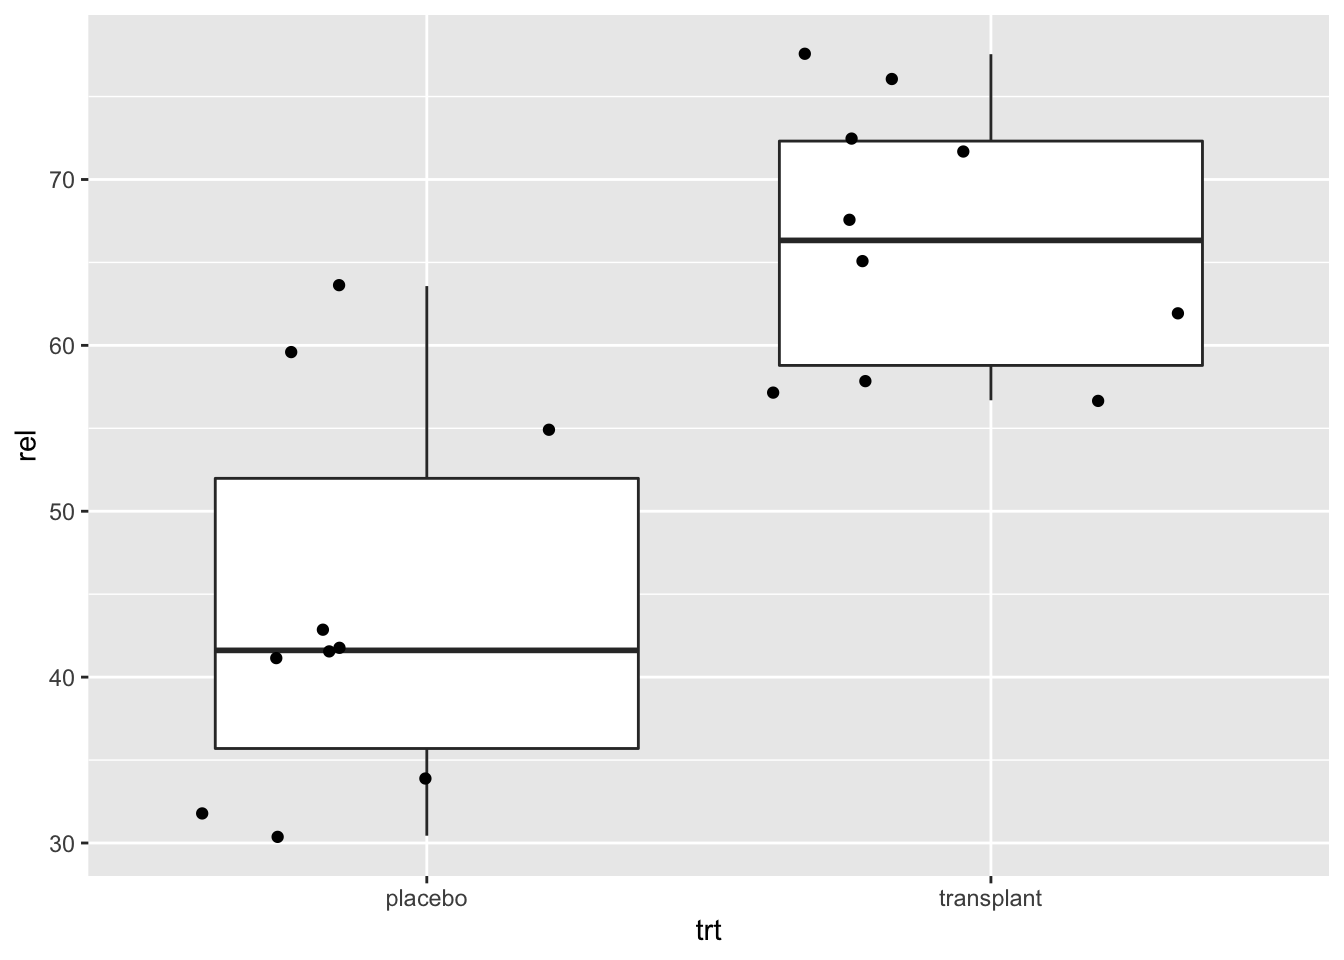
\includegraphics{Statistiek_2020_2021_files/figure-latex/unnamed-chunk-12-1.pdf}

\emph{Interpretatie}

\begin{itemize}
\tightlist
\item
  Zoals we verwachten ligt de verdeling van de lengte van mannen hoger dan deze van vrouwen.
\item
  We zien dat de data min of meer symmetrisch verdeeld zijn in elke groep en een klokvorm hebben.
\item
  We zullen later zien dat de lengte data approximatief normaal verdeeld zijn.
\item
  Dat zal ons toe laten om de data verder samen te vatten door gebruik te maken van twee statistieken: het gemiddelde en de standaard deviatie wat een maat is voor de spreiding van de gegevens rond het gemiddelde.
\end{itemize}

We maken nu een subset van de data die we zullen gebruiken om aan te tonen hoe de variabiliteit in kleine steekproeven kan variëren van steekproef tot steekproef.

\emph{Code}

\begin{enumerate}
\def\labelenumi{\arabic{enumi}.}
\tightlist
\item
  We filteren op leeftijd en verwijderen ontbrekenden gegevens (NA, Not Available).
\item
  We selecteren enkel het geslacht en Lengte zodat de dataset geen onnodige variabelen bevat.
\end{enumerate}

\begin{Shaded}
\begin{Highlighting}[]
\NormalTok{nhanesSub \textless{}{-}}\StringTok{ }\NormalTok{NHANES }\OperatorTok{\%\textgreater{}\%}\StringTok{ }\KeywordTok{filter}\NormalTok{(Age }\OperatorTok{\textgreater{}=}\StringTok{ }\DecValTok{18} \OperatorTok{\&}\StringTok{ }\OperatorTok{!}\KeywordTok{is.na}\NormalTok{(Height)) }\OperatorTok{\%\textgreater{}\%}\StringTok{ }
\StringTok{    }\KeywordTok{select}\NormalTok{(}\KeywordTok{c}\NormalTok{(}\StringTok{"Gender"}\NormalTok{, }\StringTok{"Height"}\NormalTok{))}
\end{Highlighting}
\end{Shaded}

We berekenen het gemiddelde en de standaard deviatie voor de lengte voor mannen en vrouwen in de grote dataset.
We groeperen de data hiervoor op basis van het geslacht (variable Gender).

\begin{Shaded}
\begin{Highlighting}[]
\NormalTok{HeightSum \textless{}{-}}\StringTok{ }\NormalTok{nhanesSub }\OperatorTok{\%\textgreater{}\%}\StringTok{ }\KeywordTok{group\_by}\NormalTok{(Gender) }\OperatorTok{\%\textgreater{}\%}\StringTok{ }\KeywordTok{summarize\_at}\NormalTok{(}\StringTok{"Height"}\NormalTok{, }
    \KeywordTok{list}\NormalTok{(}\DataTypeTok{mean =}\NormalTok{ mean, }\DataTypeTok{sd =}\NormalTok{ sd))}

\NormalTok{knitr}\OperatorTok{::}\KeywordTok{kable}\NormalTok{(HeightSum }\OperatorTok{\%\textgreater{}\%}\StringTok{ }\KeywordTok{mutate\_if}\NormalTok{(is.numeric, round, }
    \DataTypeTok{digits =} \DecValTok{1}\NormalTok{), }\StringTok{"html"}\NormalTok{)}
\end{Highlighting}
\end{Shaded}

Gender

mean

sd

female

162.1

7.3

male

175.9

7.5

\emph{Interpretatie}

Vrouwen zijn gemiddeld 162.1 cm HeightSum en mannen 175.9 cm.
Wat onze intuïtie bevestigt dat mannen gemiddeld groter zijn dan vrouwen.

\hypertarget{experiment}{%
\subsection{Experiment}\label{experiment}}

\begin{itemize}
\item
  Stel dat we geen toegang hebben tot de metingen van de NHANES studie.
\item
  We zouden dan een experiment op moeten zetten om metingen bij mannen en vrouwen te doen.
\item
  Veronderstel dat we budget hebben om metingen bij 5 mannen en 5 vrouwen te doen.
\item
  We zouden dan 5 mannen en 5 vrouwen boven de 25 jaar at random selecteren uit de Amerikaanse populatie.
\item
  We kunnen dit experiment simuleren door 5 vrouwen en 5 mannen at random te selecteren uit de NHANES studie.
\end{itemize}

\emph{Code}

\begin{verbatim}
1. het `set.seed` commando wordt gebruikt omdat we dezelfde steekproef zou trekken als we de code opnieuw laten lopen. Dit is louter om de cursus consistent te houden als we de nota's opnieuw maken.
2. het nSamp object bevat de steekproefgrootte per groep
3. we trekken 5 vrouwelijke subjecten uit de nhanesSub dataset
4. vervolgens trekken we 5 mannen uit de nhanesSub dataset
5. we voegen de data van mannen en vrouwen samen in 1 dataset. Het `rbind` commando zal de data van de rijen onder elkaar zetten.
6. We tonen de dataset
\end{verbatim}

\begin{Shaded}
\begin{Highlighting}[]
\KeywordTok{set.seed}\NormalTok{(}\DecValTok{1023}\NormalTok{)}
\NormalTok{nSamp \textless{}{-}}\StringTok{ }\DecValTok{5}
\NormalTok{fem \textless{}{-}}\StringTok{ }\NormalTok{nhanesSub }\OperatorTok{\%\textgreater{}\%}\StringTok{ }\KeywordTok{filter}\NormalTok{(Gender }\OperatorTok{==}\StringTok{ "female"}\NormalTok{) }\OperatorTok{\%\textgreater{}\%}\StringTok{ }
\StringTok{    }\KeywordTok{sample\_n}\NormalTok{(}\DataTypeTok{size =} \DecValTok{5}\NormalTok{)}

\NormalTok{mal \textless{}{-}}\StringTok{ }\NormalTok{nhanesSub }\OperatorTok{\%\textgreater{}\%}\StringTok{ }\KeywordTok{filter}\NormalTok{(Gender }\OperatorTok{==}\StringTok{ "male"}\NormalTok{) }\OperatorTok{\%\textgreater{}\%}\StringTok{ }\KeywordTok{sample\_n}\NormalTok{(}\DataTypeTok{size =} \DecValTok{5}\NormalTok{)}

\NormalTok{samp1 \textless{}{-}}\StringTok{ }\KeywordTok{rbind}\NormalTok{(fem, mal)}

\NormalTok{samp1}
\end{Highlighting}
\end{Shaded}

\begin{verbatim}
## # A tibble: 10 x 2
##    Gender Height
##    <fct>   <dbl>
##  1 female   164 
##  2 female   160.
##  3 female   159 
##  4 female   154.
##  5 female   156.
##  6 male     170.
##  7 male     183.
##  8 male     183.
##  9 male     185.
## 10 male     170.
\end{verbatim}

We hebben met de code dus een steekproef getrokken van 5 vrouwen en 5 mannen.
We exploreren vervolgens de data in de steekproef.

\emph{Code}

\begin{Shaded}
\begin{Highlighting}[]
\NormalTok{samp1 }\OperatorTok{\%\textgreater{}\%}\StringTok{ }\KeywordTok{ggplot}\NormalTok{(}\KeywordTok{aes}\NormalTok{(}\DataTypeTok{x =}\NormalTok{ Height)) }\OperatorTok{+}\StringTok{ }\KeywordTok{geom\_histogram}\NormalTok{() }\OperatorTok{+}\StringTok{ }
\StringTok{    }\KeywordTok{facet\_grid}\NormalTok{(Gender }\OperatorTok{\textasciitilde{}}\StringTok{ }\NormalTok{.) }\OperatorTok{+}\StringTok{ }\KeywordTok{xlab}\NormalTok{(}\StringTok{"Lengte (cm)"}\NormalTok{)}
\end{Highlighting}
\end{Shaded}

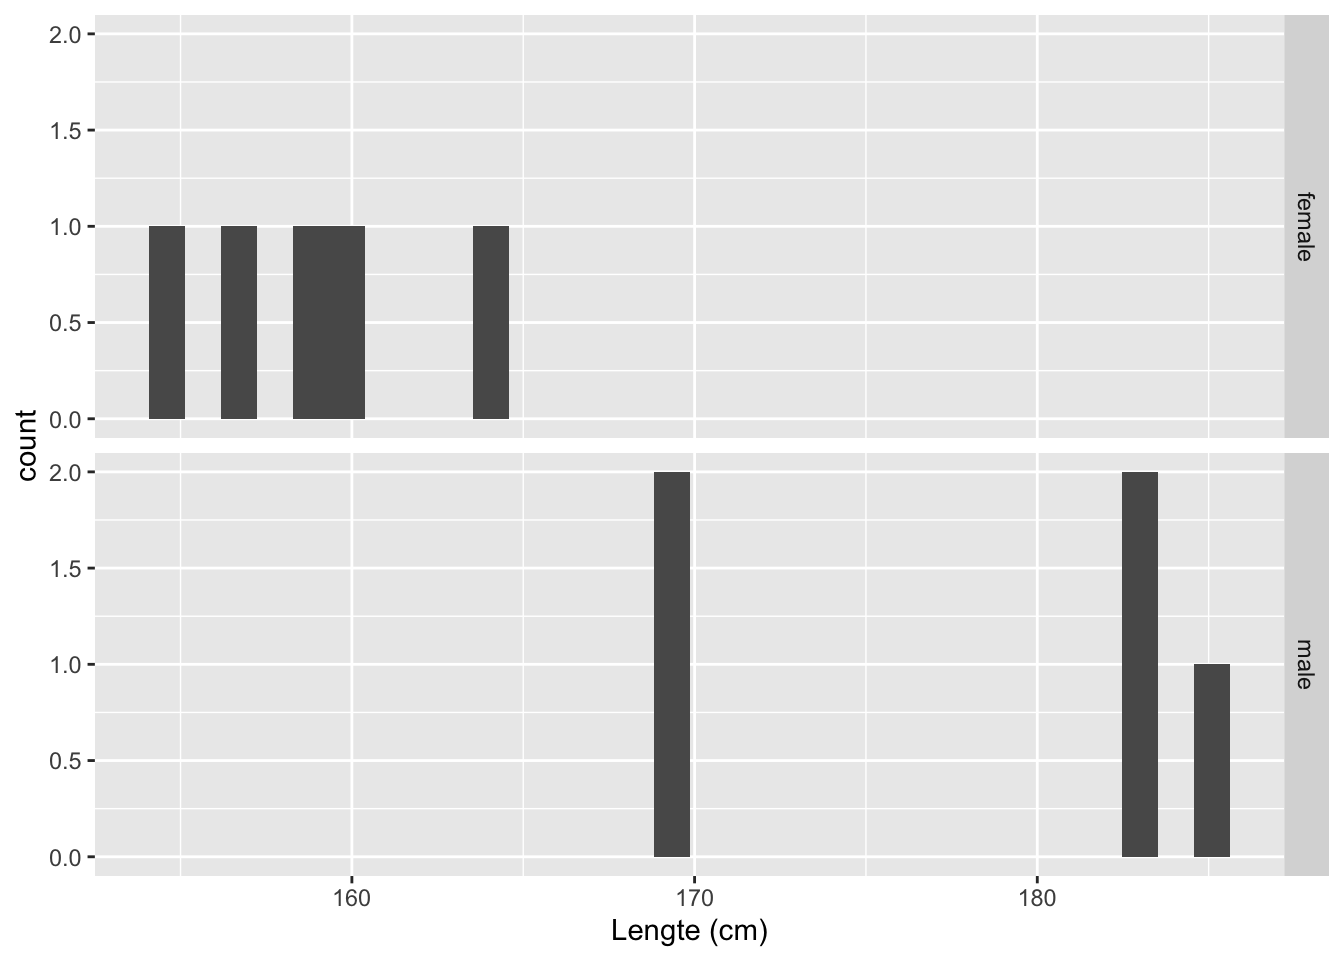
\includegraphics{Statistiek_2020_2021_files/figure-latex/unnamed-chunk-16-1.pdf}

\begin{Shaded}
\begin{Highlighting}[]
\NormalTok{HeightSumExp1 \textless{}{-}}\StringTok{ }\NormalTok{samp1 }\OperatorTok{\%\textgreater{}\%}\StringTok{ }\KeywordTok{group\_by}\NormalTok{(Gender) }\OperatorTok{\%\textgreater{}\%}\StringTok{ }\KeywordTok{summarize\_at}\NormalTok{(}\StringTok{"Height"}\NormalTok{, }
    \KeywordTok{list}\NormalTok{(}\DataTypeTok{mean =}\NormalTok{ mean, }\DataTypeTok{sd =}\NormalTok{ sd))}
\NormalTok{HeightSumExp1}
\end{Highlighting}
\end{Shaded}

\begin{verbatim}
## # A tibble: 2 x 3
##   Gender  mean    sd
##   <fct>  <dbl> <dbl>
## 1 female  159.  3.76
## 2 male    178.  7.55
\end{verbatim}

Histogram is niet zinvol als we maar zo weinig datapunten hebben. Een boxplot is meer geschikt om distributies te vergelijken als er weinig data zijn:

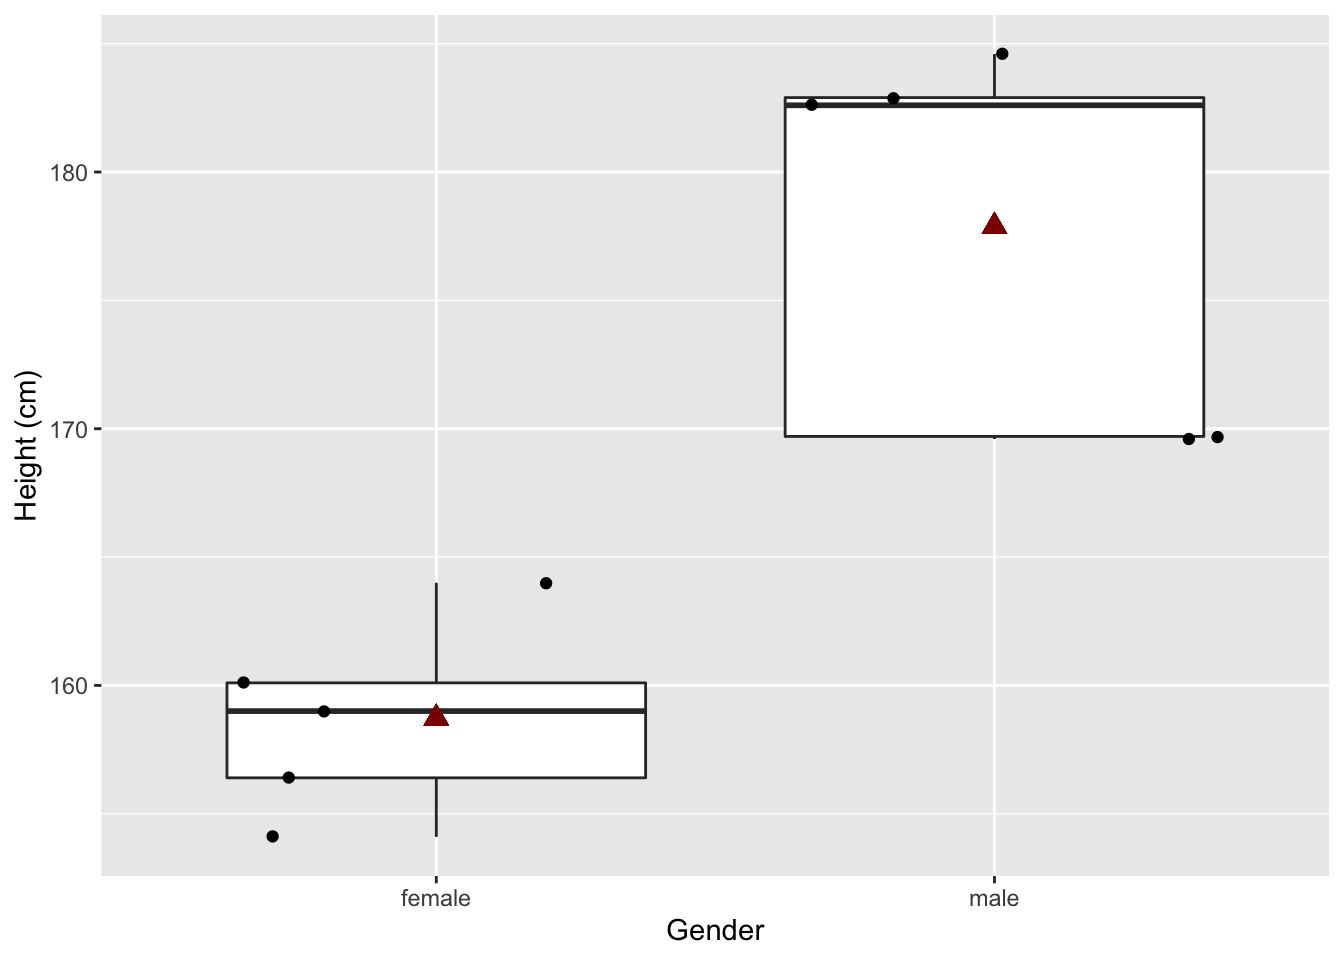
\includegraphics{Statistiek_2020_2021_files/figure-latex/unnamed-chunk-17-1.pdf}

\emph{Einde Code}

Om na te gaan of het verschil in de steekproef groot genoeg is om de bevindingen van de steekproef te kunnen veralgemenen naar de populatie toe voeren we opnieuw een t-test uit.

Met de p-waarde wordt de kans berekend om in een nieuwe random steekproef door toeval een effect te vinden dat in absolute waarde minstens evengroot is als in onze geobserveerde steekproef onder de aanname dat er in werkelijkheid geen verschil zou zijn in gemiddelde lengte tussen vrouwen en mannen.

Als die kans heel klein is is het weinig waarschijnlijk om onze steekproef te observeren onder de hypothese dat de lengtes gemiddeld niet verschillen tussen vrouwen en mannen en kunnen we deze hypothese verwerpen.

Typisch wordt de kans op een valse positieve conclusie gecontroleerd op 5\%.

\begin{Shaded}
\begin{Highlighting}[]
\KeywordTok{t.test}\NormalTok{(Height }\OperatorTok{\textasciitilde{}}\StringTok{ }\NormalTok{Gender, }\DataTypeTok{data =}\NormalTok{ samp1)}
\end{Highlighting}
\end{Shaded}

\begin{verbatim}
## 
## 	Welch Two Sample t-test
## 
## data:  Height by Gender
## t = -5.0783, df = 5.8695, p-value = 0.00242
## alternative hypothesis: true difference in means is not equal to 0
## 95 percent confidence interval:
##  -28.441927  -9.878073
## sample estimates:
## mean in group female   mean in group male 
##               158.72               177.88
\end{verbatim}

In het experiment zijn vrouwen gemiddeld 19.16 cm kleiner dan mannen. En als we een statistische test uitvoeren (zie hoofdstuk 5: Statistische besluitvorming) kunnen we besluiten dat dit verschil statistisch significant is.

\hypertarget{herhaal-het-experiment}{%
\subsection{Herhaal het experiment}\label{herhaal-het-experiment}}

Als we het experiment herhalen selecteren we andere mensen en verkrijgen we andere resultaten.

\begin{Shaded}
\begin{Highlighting}[]
\KeywordTok{set.seed}\NormalTok{(}\DecValTok{1024}\NormalTok{)}
\NormalTok{fem \textless{}{-}}\StringTok{ }\NormalTok{nhanesSub }\OperatorTok{\%\textgreater{}\%}\StringTok{ }\KeywordTok{filter}\NormalTok{(Gender }\OperatorTok{==}\StringTok{ "female"}\NormalTok{) }\OperatorTok{\%\textgreater{}\%}\StringTok{ }
\StringTok{    }\KeywordTok{sample\_n}\NormalTok{(}\DataTypeTok{size =} \DecValTok{5}\NormalTok{)}

\NormalTok{mal \textless{}{-}}\StringTok{ }\NormalTok{nhanesSub }\OperatorTok{\%\textgreater{}\%}\StringTok{ }\KeywordTok{filter}\NormalTok{(Gender }\OperatorTok{==}\StringTok{ "male"}\NormalTok{) }\OperatorTok{\%\textgreater{}\%}\StringTok{ }\KeywordTok{sample\_n}\NormalTok{(}\DataTypeTok{size =} \DecValTok{5}\NormalTok{)}

\NormalTok{samp2 \textless{}{-}}\StringTok{ }\KeywordTok{rbind}\NormalTok{(fem, mal)}

\NormalTok{HeightSumExp2 \textless{}{-}}\StringTok{ }\NormalTok{samp2 }\OperatorTok{\%\textgreater{}\%}\StringTok{ }\KeywordTok{group\_by}\NormalTok{(Gender) }\OperatorTok{\%\textgreater{}\%}\StringTok{ }\KeywordTok{summarize\_at}\NormalTok{(}\StringTok{"Height"}\NormalTok{, }
    \KeywordTok{list}\NormalTok{(}\DataTypeTok{mean =}\NormalTok{ mean, }\DataTypeTok{sd =}\NormalTok{ sd))}
\NormalTok{HeightSumExp2}
\end{Highlighting}
\end{Shaded}

\begin{verbatim}
## # A tibble: 2 x 3
##   Gender  mean    sd
##   <fct>  <dbl> <dbl>
## 1 female  166.  9.89
## 2 male    170.  8.24
\end{verbatim}

\begin{Shaded}
\begin{Highlighting}[]
\NormalTok{samp2 }\OperatorTok{\%\textgreater{}\%}\StringTok{ }\KeywordTok{ggplot}\NormalTok{(}\KeywordTok{aes}\NormalTok{(}\DataTypeTok{x =}\NormalTok{ Gender, }\DataTypeTok{y =}\NormalTok{ Height)) }\OperatorTok{+}\StringTok{ }\KeywordTok{geom\_boxplot}\NormalTok{(}\DataTypeTok{outlier.shape =} \OtherTok{NA}\NormalTok{) }\OperatorTok{+}\StringTok{ }
\StringTok{    }\KeywordTok{geom\_point}\NormalTok{(}\DataTypeTok{position =} \StringTok{"jitter"}\NormalTok{) }\OperatorTok{+}\StringTok{ }\KeywordTok{geom\_point}\NormalTok{(}\KeywordTok{aes}\NormalTok{(}\DataTypeTok{x =} \DecValTok{1}\NormalTok{, }
    \DataTypeTok{y =}\NormalTok{ HeightSumExp2}\OperatorTok{$}\NormalTok{mean[}\DecValTok{1}\NormalTok{]), }\DataTypeTok{size =} \DecValTok{3}\NormalTok{, }\DataTypeTok{pch =} \DecValTok{17}\NormalTok{, }
    \DataTypeTok{color =} \StringTok{"darkred"}\NormalTok{) }\OperatorTok{+}\StringTok{ }\KeywordTok{geom\_point}\NormalTok{(}\KeywordTok{aes}\NormalTok{(}\DataTypeTok{x =} \DecValTok{2}\NormalTok{, }\DataTypeTok{y =}\NormalTok{ HeightSumExp2}\OperatorTok{$}\NormalTok{mean[}\DecValTok{2}\NormalTok{]), }
    \DataTypeTok{size =} \DecValTok{3}\NormalTok{, }\DataTypeTok{pch =} \DecValTok{17}\NormalTok{, }\DataTypeTok{color =} \StringTok{"darkred"}\NormalTok{) }\OperatorTok{+}\StringTok{ }\KeywordTok{ylab}\NormalTok{(}\StringTok{"Height (cm)"}\NormalTok{)}
\end{Highlighting}
\end{Shaded}

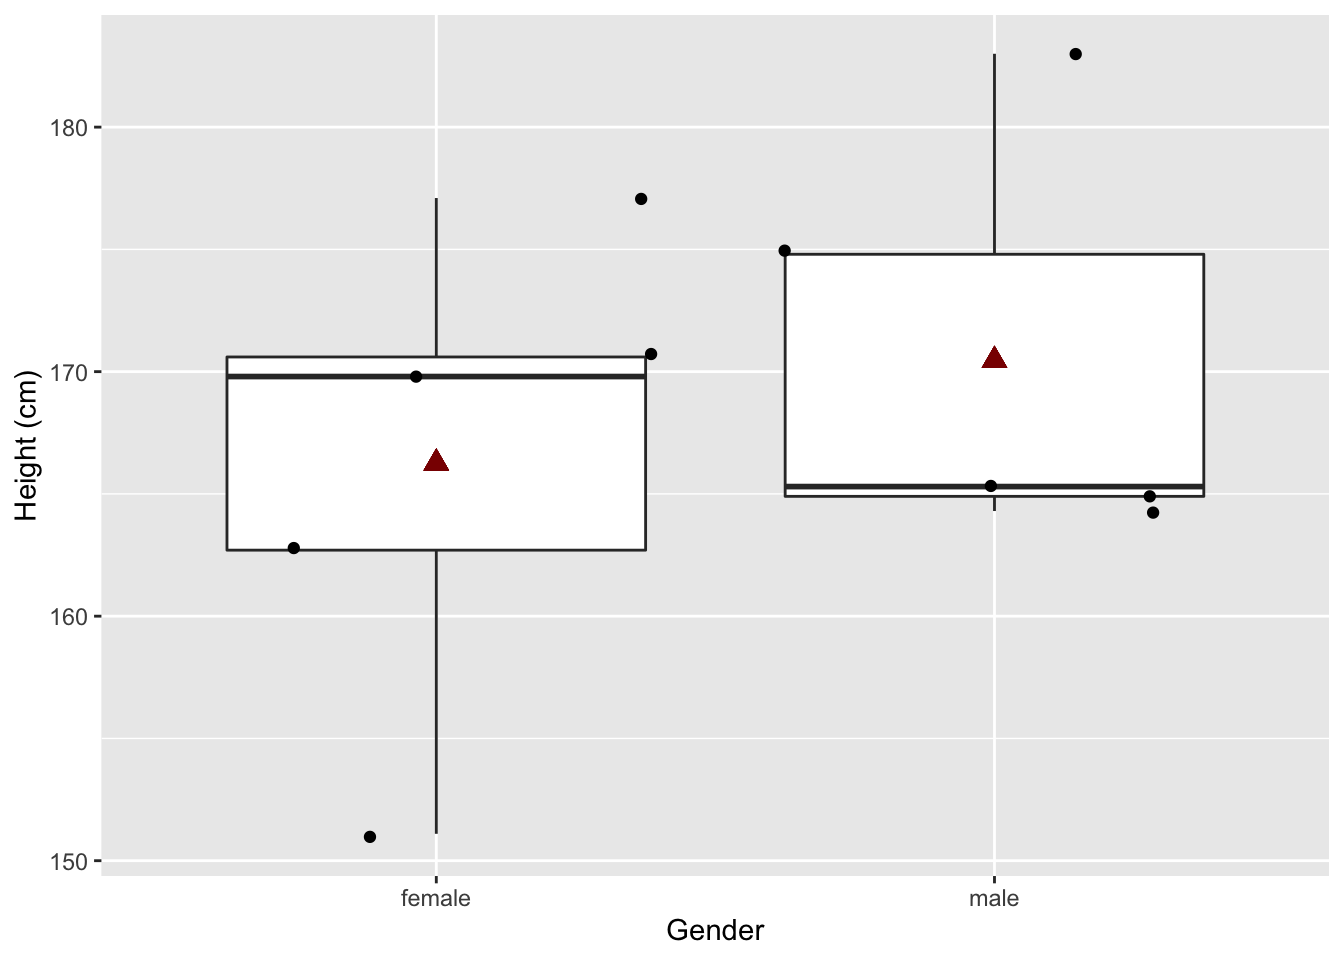
\includegraphics{Statistiek_2020_2021_files/figure-latex/unnamed-chunk-19-1.pdf}

\begin{Shaded}
\begin{Highlighting}[]
\KeywordTok{t.test}\NormalTok{(Height }\OperatorTok{\textasciitilde{}}\StringTok{ }\NormalTok{Gender, }\DataTypeTok{data =}\NormalTok{ samp2)}
\end{Highlighting}
\end{Shaded}

\begin{verbatim}
## 
## 	Welch Two Sample t-test
## 
## data:  Height by Gender
## t = -0.7295, df = 7.747, p-value = 0.4872
## alternative hypothesis: true difference in means is not equal to 0
## 95 percent confidence interval:
##  -17.552343   9.152343
## sample estimates:
## mean in group female   mean in group male 
##               166.26               170.46
\end{verbatim}

Vijf andere mannen en vrouwen worden getrokken uit de populatie. Hierdoor verschillen de lengte metingen van de vorige steekproef alsook de berekende gemiddeldes en de p-waarde van de statistische toets.

In de nieuwe steekproef zijn vrouwen gemiddeld 4.2 cm kleiner dan mannen. En dit verschil is statistisch niet significant

\hypertarget{herhaal-het-experiment-opnieuw}{%
\subsection{Herhaal het experiment opnieuw}\label{herhaal-het-experiment-opnieuw}}

\begin{Shaded}
\begin{Highlighting}[]
\NormalTok{seed \textless{}{-}}\StringTok{ }\DecValTok{88605}
\KeywordTok{set.seed}\NormalTok{(seed)}
\NormalTok{fem \textless{}{-}}\StringTok{ }\NormalTok{nhanesSub }\OperatorTok{\%\textgreater{}\%}\StringTok{ }\KeywordTok{filter}\NormalTok{(Gender }\OperatorTok{==}\StringTok{ "female"}\NormalTok{) }\OperatorTok{\%\textgreater{}\%}\StringTok{ }
\StringTok{    }\KeywordTok{sample\_n}\NormalTok{(}\DataTypeTok{size =} \DecValTok{5}\NormalTok{)}

\NormalTok{mal \textless{}{-}}\StringTok{ }\NormalTok{nhanesSub }\OperatorTok{\%\textgreater{}\%}\StringTok{ }\KeywordTok{filter}\NormalTok{(Gender }\OperatorTok{==}\StringTok{ "male"}\NormalTok{) }\OperatorTok{\%\textgreater{}\%}\StringTok{ }\KeywordTok{sample\_n}\NormalTok{(}\DataTypeTok{size =} \DecValTok{5}\NormalTok{)}

\NormalTok{samp3 \textless{}{-}}\StringTok{ }\KeywordTok{rbind}\NormalTok{(fem, mal)}

\NormalTok{HeightSumExp3 \textless{}{-}}\StringTok{ }\NormalTok{samp3 }\OperatorTok{\%\textgreater{}\%}\StringTok{ }\KeywordTok{group\_by}\NormalTok{(Gender) }\OperatorTok{\%\textgreater{}\%}\StringTok{ }\KeywordTok{summarize\_at}\NormalTok{(}\StringTok{"Height"}\NormalTok{, }
    \KeywordTok{list}\NormalTok{(}\DataTypeTok{mean =}\NormalTok{ mean, }\DataTypeTok{sd =}\NormalTok{ sd))}
\NormalTok{HeightSumExp3}
\end{Highlighting}
\end{Shaded}

\begin{verbatim}
## # A tibble: 2 x 3
##   Gender  mean    sd
##   <fct>  <dbl> <dbl>
## 1 female  173.  1.97
## 2 male    168.  2.84
\end{verbatim}

\begin{Shaded}
\begin{Highlighting}[]
\NormalTok{samp3 }\OperatorTok{\%\textgreater{}\%}\StringTok{ }\KeywordTok{ggplot}\NormalTok{(}\KeywordTok{aes}\NormalTok{(}\DataTypeTok{x =}\NormalTok{ Gender, }\DataTypeTok{y =}\NormalTok{ Height)) }\OperatorTok{+}\StringTok{ }\KeywordTok{geom\_boxplot}\NormalTok{(}\DataTypeTok{outlier.shape =} \OtherTok{NA}\NormalTok{) }\OperatorTok{+}\StringTok{ }
\StringTok{    }\KeywordTok{geom\_point}\NormalTok{(}\DataTypeTok{position =} \StringTok{"jitter"}\NormalTok{) }\OperatorTok{+}\StringTok{ }\KeywordTok{geom\_point}\NormalTok{(}\KeywordTok{aes}\NormalTok{(}\DataTypeTok{x =} \DecValTok{1}\NormalTok{, }
    \DataTypeTok{y =}\NormalTok{ HeightSumExp3}\OperatorTok{$}\NormalTok{mean[}\DecValTok{1}\NormalTok{]), }\DataTypeTok{size =} \DecValTok{3}\NormalTok{, }\DataTypeTok{pch =} \DecValTok{17}\NormalTok{, }
    \DataTypeTok{color =} \StringTok{"darkred"}\NormalTok{) }\OperatorTok{+}\StringTok{ }\KeywordTok{geom\_point}\NormalTok{(}\KeywordTok{aes}\NormalTok{(}\DataTypeTok{x =} \DecValTok{2}\NormalTok{, }\DataTypeTok{y =}\NormalTok{ HeightSumExp3}\OperatorTok{$}\NormalTok{mean[}\DecValTok{2}\NormalTok{]), }
    \DataTypeTok{size =} \DecValTok{3}\NormalTok{, }\DataTypeTok{pch =} \DecValTok{17}\NormalTok{, }\DataTypeTok{color =} \StringTok{"darkred"}\NormalTok{) }\OperatorTok{+}\StringTok{ }\KeywordTok{ylab}\NormalTok{(}\StringTok{"Height (cm)"}\NormalTok{)}
\end{Highlighting}
\end{Shaded}

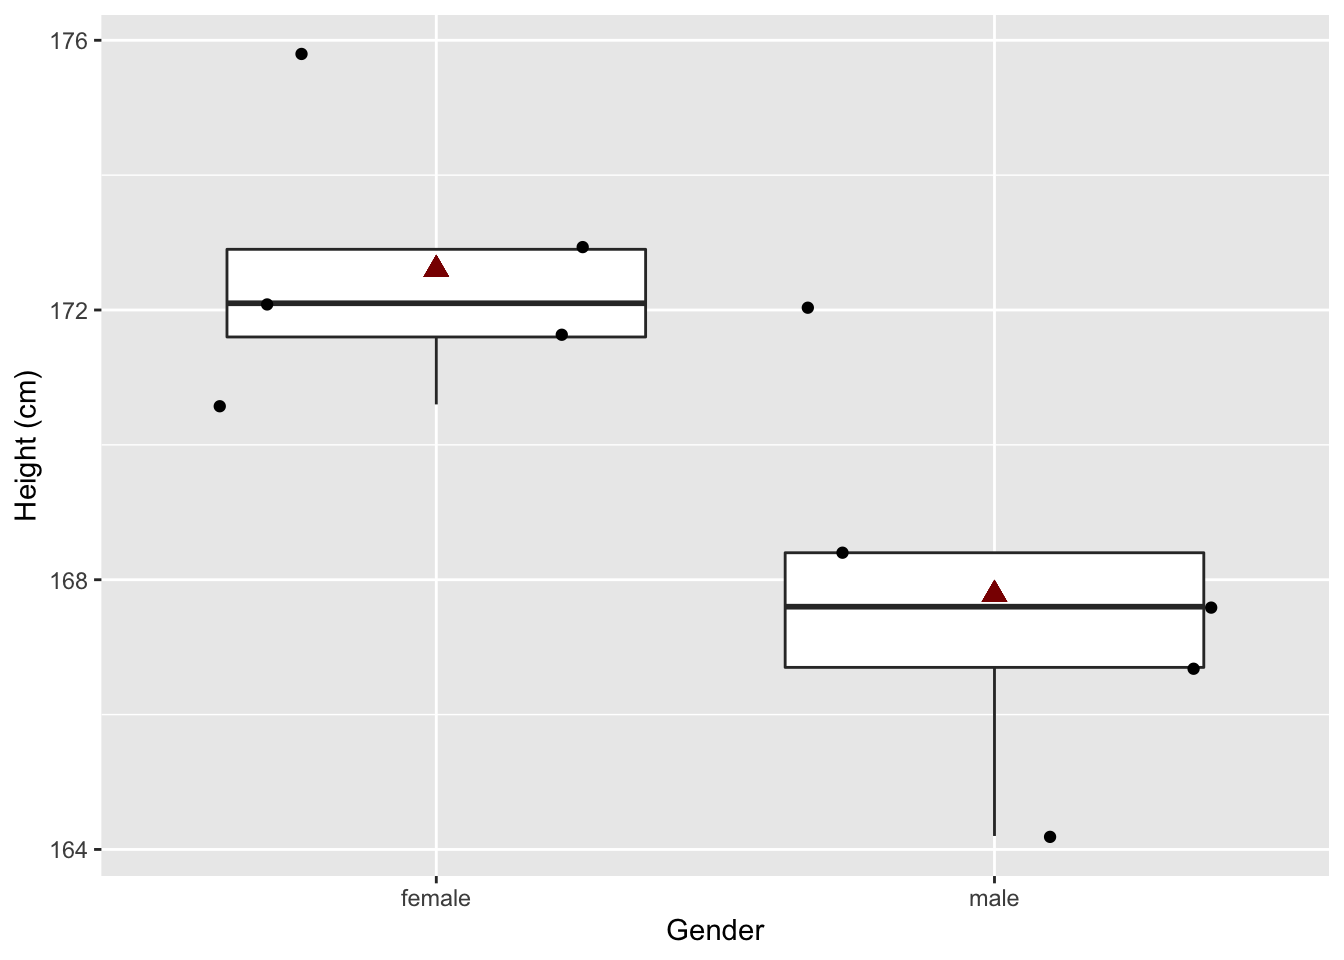
\includegraphics{Statistiek_2020_2021_files/figure-latex/unnamed-chunk-20-1.pdf}

\begin{Shaded}
\begin{Highlighting}[]
\KeywordTok{t.test}\NormalTok{(Height }\OperatorTok{\textasciitilde{}}\StringTok{ }\NormalTok{Gender, }\DataTypeTok{data =}\NormalTok{ samp3)}
\end{Highlighting}
\end{Shaded}

\begin{verbatim}
## 
## 	Welch Two Sample t-test
## 
## data:  Height by Gender
## t = 3.1182, df = 7.136, p-value = 0.01648
## alternative hypothesis: true difference in means is not equal to 0
## 95 percent confidence interval:
##  1.178916 8.461084
## sample estimates:
## mean in group female   mean in group male 
##               172.60               167.78
\end{verbatim}

In de nieuwe steekproef zijn vrouwen gemiddeld 4.82 cm groter dan mannen. En dit verschil is statistisch significant

Merk op dat we in deze extreme steekproef door toeval vrij grote vrouwen en eerder kleine mannen hebben getrokken uit de populatie. Een dergelijke steekproef zal eerder zeldzaam zijn maar kan door toeval voorkomen.

In de onderstaande paragraaf leggen we uit hoe we deze extreme steekproef hebben bekomen:

Een seed wordt in de cursus gebruikt om ervoor te zorgen dat we telkens dezelfde resultaten bekomen als we de random generator opnieuw laten lopen in R (zie het set.seed commando). Dat doen we puur om de resultaten in de cursus gelijk te kunnen houden als we aanpassingen hebben doorgevoerd aan de tekst en de code dus opnieuw moeten laten lopen om de cursus te compileren. In vrijwel alle code is de seed gewoon random gekozen.

Om de extreme steekproef weer te geven, hebben we deze keer echter geen random seed gebruikt. Daarvoor hebben we alle seeds overlopen van 1 tot 100000. We hebben dus \ensuremath{8.8605\times 10^{4}} steekproeven moeten trekken alvorens we een dergelijke extreme steekproef uit de populatie hadden getrokken waaruit we ten onrechte zouden concluderen dat vrouwen gemiddeld significant groter zijn dan mannen.

\hypertarget{samenvatting}{%
\subsection{Samenvatting}\label{samenvatting}}

We trokken at random andere proefpersonen in elke steekproef. Hierdoor

\begin{itemize}
\item
  verschillen de lengtemetingen van steekproef tot steekproef.
\item
  Dus ook de geschatte gemiddeldes en standaard deviaties.
\item
  Bijgevolg zijn onze conclusies ook onzeker en kunnen deze wijzigen van steekproef tot steekproef.
\item
  Ook steekproeven waarbij het effect tegengesteld is aan dat in de populatie en waarbij we besluiten dat het verschil significant is kunnen voorkomen.
\item
  We kunnen aantonen dat dergelijke steekproeven voor experimenten waarbij we de lengte tussen mannen en vrouwen vergelijken eerder zeldzaam zijn.
\end{itemize}

\(\rightarrow\) Met statistiek gaan we de kans op het trekken foute conclusies controleren.

\hypertarget{controle-van-beslissingsfouten}{%
\subsection{Controle van beslissingsfouten}\label{controle-van-beslissingsfouten}}

Hoe controleert statistiek de kans op het trekken van foute conclusies?

\begin{itemize}
\tightlist
\item
  In onderstaande code trekken we 10000 herhaalde steekproeven van 5 vrouwen en 5 mannen uit de NHANES studie.
\end{itemize}

\emph{Code}

Deze code is vrij complex. Het kan nuttig zijn om deze pas na de twee modules Introductie tot R, en, data visualisatie opnieuw te bekijken.

\begin{Shaded}
\begin{Highlighting}[]
\KeywordTok{set.seed}\NormalTok{(}\DecValTok{15152}\NormalTok{)}
\CommentTok{\# Aantal simulaties en steekproefgrootte per groep}
\NormalTok{nSim \textless{}{-}}\StringTok{ }\DecValTok{10000}
\NormalTok{nSamp \textless{}{-}}\StringTok{ }\DecValTok{5}

\CommentTok{\# We filteren de data vooraf zodat we dit niet}
\CommentTok{\# telkens opnieuw hoeven te doen}
\NormalTok{fem \textless{}{-}}\StringTok{ }\NormalTok{nhanesSub }\OperatorTok{\%\textgreater{}\%}\StringTok{ }\KeywordTok{filter}\NormalTok{(Gender }\OperatorTok{==}\StringTok{ "female"}\NormalTok{)}

\NormalTok{mal \textless{}{-}}\StringTok{ }\NormalTok{nhanesSub }\OperatorTok{\%\textgreater{}\%}\StringTok{ }\KeywordTok{filter}\NormalTok{(Gender }\OperatorTok{==}\StringTok{ "male"}\NormalTok{)}

\CommentTok{\# Simulatie studie Om snelle functies te kunnen}
\CommentTok{\# gebruiken nemen we eerst nSim steekproeven en}
\CommentTok{\# berekenen we daarna alles.}

\NormalTok{femSamps \textless{}{-}}\StringTok{ }\NormalTok{malSamps \textless{}{-}}\StringTok{ }\KeywordTok{matrix}\NormalTok{(}\OtherTok{NA}\NormalTok{, }\DataTypeTok{nrow =}\NormalTok{ nSamp, }\DataTypeTok{ncol =}\NormalTok{ nSim)}
\ControlFlowTok{for}\NormalTok{ (i }\ControlFlowTok{in} \DecValTok{1}\OperatorTok{:}\NormalTok{nSim) \{}
\NormalTok{    femSamps[, i] \textless{}{-}}\StringTok{ }\KeywordTok{sample}\NormalTok{(fem}\OperatorTok{$}\NormalTok{Height, nSamp)}
\NormalTok{    malSamps[, i] \textless{}{-}}\StringTok{ }\KeywordTok{sample}\NormalTok{(mal}\OperatorTok{$}\NormalTok{Height, nSamp)}
\NormalTok{\}}

\NormalTok{res \textless{}{-}}\StringTok{ }\KeywordTok{data.frame}\NormalTok{(}\DataTypeTok{verschil =} \KeywordTok{colMeans}\NormalTok{(femSamps) }\OperatorTok{{-}}\StringTok{ }\KeywordTok{colMeans}\NormalTok{(malSamps), }
\NormalTok{    Rfast}\OperatorTok{::}\KeywordTok{ttests}\NormalTok{(femSamps, malSamps))}

\KeywordTok{sum}\NormalTok{(res}\OperatorTok{$}\NormalTok{pvalue }\OperatorTok{\textless{}}\StringTok{ }\FloatTok{0.05} \OperatorTok{\&}\StringTok{ }\NormalTok{res}\OperatorTok{$}\NormalTok{verschil }\OperatorTok{\textless{}}\StringTok{ }\DecValTok{0}\NormalTok{)}
\end{Highlighting}
\end{Shaded}

\begin{verbatim}
## [1] 7234
\end{verbatim}

\begin{Shaded}
\begin{Highlighting}[]
\KeywordTok{sum}\NormalTok{(res}\OperatorTok{$}\NormalTok{pvalue }\OperatorTok{\textgreater{}=}\StringTok{ }\FloatTok{0.05}\NormalTok{)}
\end{Highlighting}
\end{Shaded}

\begin{verbatim}
## [1] 2766
\end{verbatim}

\begin{Shaded}
\begin{Highlighting}[]
\KeywordTok{sum}\NormalTok{(res}\OperatorTok{$}\NormalTok{pvalue }\OperatorTok{\textless{}}\StringTok{ }\FloatTok{0.05} \OperatorTok{\&}\StringTok{ }\NormalTok{res}\OperatorTok{$}\NormalTok{verschil }\OperatorTok{\textgreater{}}\StringTok{ }\DecValTok{0}\NormalTok{)}
\end{Highlighting}
\end{Shaded}

\begin{verbatim}
## [1] 0
\end{verbatim}

\begin{Shaded}
\begin{Highlighting}[]
\NormalTok{res }\OperatorTok{\%\textgreater{}\%}\StringTok{ }\KeywordTok{ggplot}\NormalTok{(}\KeywordTok{aes}\NormalTok{(}\DataTypeTok{x =}\NormalTok{ verschil, }\DataTypeTok{y =} \OperatorTok{{-}}\KeywordTok{log10}\NormalTok{(pvalue), }
    \DataTypeTok{color =}\NormalTok{ pvalue }\OperatorTok{\textless{}}\StringTok{ }\FloatTok{0.05}\NormalTok{)) }\OperatorTok{+}\StringTok{ }\KeywordTok{geom\_point}\NormalTok{() }\OperatorTok{+}\StringTok{ }\KeywordTok{xlab}\NormalTok{(}\StringTok{"Gemiddeld Verschil (cm)"}\NormalTok{) }\OperatorTok{+}\StringTok{ }
\StringTok{    }\KeywordTok{ylab}\NormalTok{(}\StringTok{"Statistische Significantie ({-}log10 p)"}\NormalTok{)}
\end{Highlighting}
\end{Shaded}

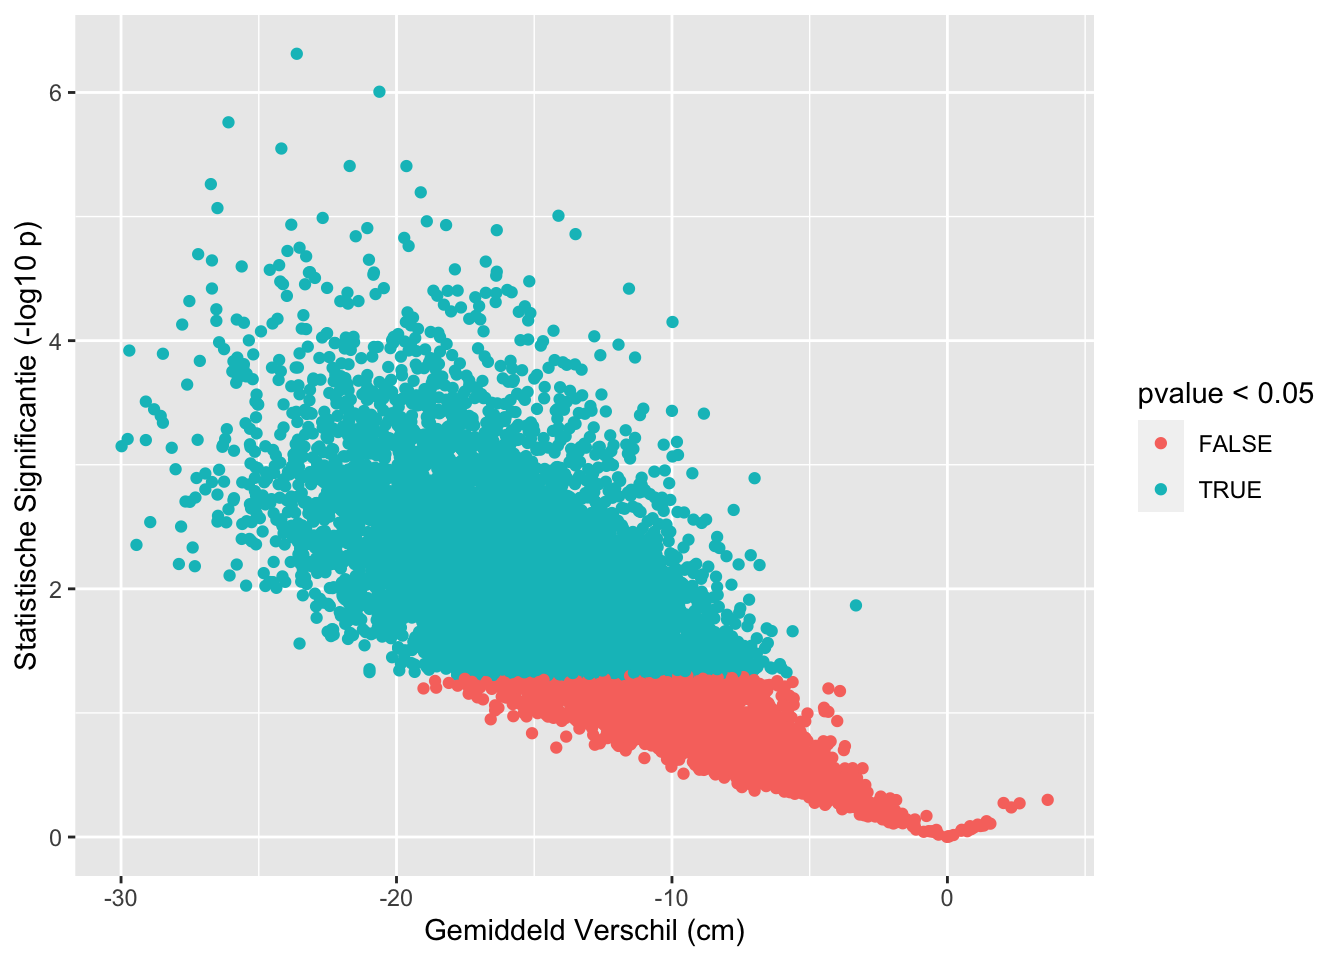
\includegraphics{Statistiek_2020_2021_files/figure-latex/unnamed-chunk-21-1.pdf}

\begin{Shaded}
\begin{Highlighting}[]
\NormalTok{res }\OperatorTok{\%\textgreater{}\%}\StringTok{ }\KeywordTok{ggplot}\NormalTok{(}\KeywordTok{aes}\NormalTok{(}\DataTypeTok{y =}\NormalTok{ verschil)) }\OperatorTok{+}\StringTok{ }\KeywordTok{geom\_boxplot}\NormalTok{() }\OperatorTok{+}\StringTok{ }
\StringTok{    }\KeywordTok{ylab}\NormalTok{(}\StringTok{"Gemiddeld Verschil (cm)"}\NormalTok{)}
\end{Highlighting}
\end{Shaded}

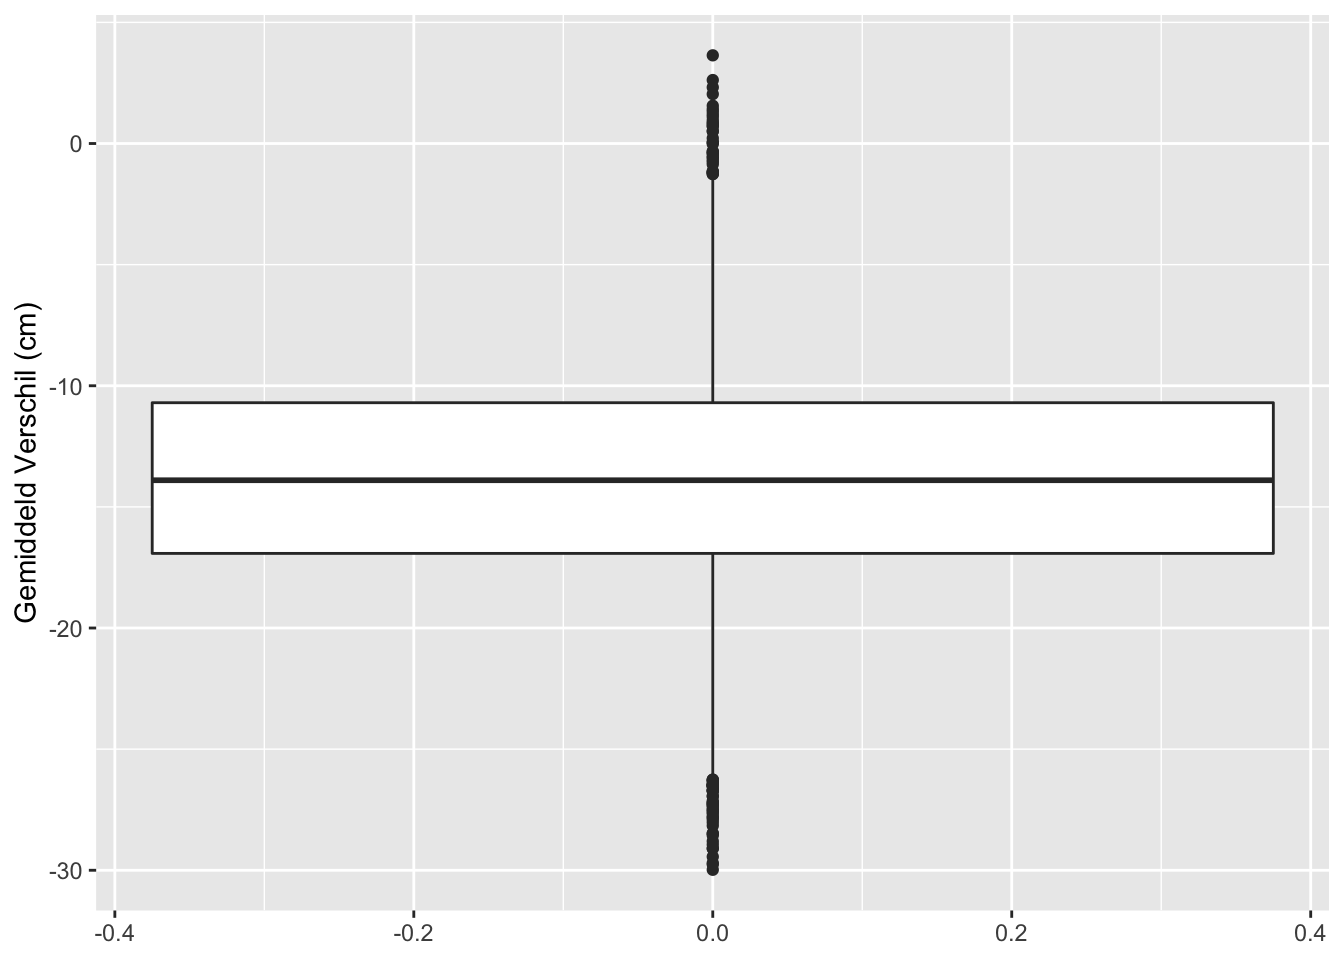
\includegraphics{Statistiek_2020_2021_files/figure-latex/unnamed-chunk-21-2.pdf}

\begin{Shaded}
\begin{Highlighting}[]
\KeywordTok{xlab}\NormalTok{(}\StringTok{""}\NormalTok{)}
\end{Highlighting}
\end{Shaded}

\begin{verbatim}
## $x
## [1] ""
## 
## attr(,"class")
## [1] "labels"
\end{verbatim}

Op basis van 10000 steekproeven van 5 mannen en 5 vrouwen zagen we dat in 7234 steekproeven vrouwen gemiddeld significant kleiner zijn dan mannen. In 2766 steekproeven besluiten we dat vrouwen en mannen gemiddeld niet significant verschillen in lengte. En in 0 besluiten we dat vrouwen gemiddeld significant groter zijn dan mannen.

\begin{itemize}
\item
  De steekproef die we toonden waaruit we zouden besluiten dat vrouwen significant groter zijn dan mannen is heel onwaarschijnlijk. Er moesten 88605 steekproeven worden getrokken om deze extreme steekproef te vinden.
\item
  Het feit dat we in veel steekproeven resultaten vinden die statistisch niet significant zijn komt omdat de statistische toets een te lage kracht heeft om het verschil te detecteren wanneer er maar 5 observaties zijn per groep.
\end{itemize}

\begin{center}\rule{0.5\linewidth}{0.5pt}\end{center}

\hypertarget{grotere-steekproef}{%
\subsubsection{Grotere steekproef?}\label{grotere-steekproef}}

Wat gebeurt er als we de steekproef verhogen naar 50 observaties per groep?

\begin{Shaded}
\begin{Highlighting}[]
\KeywordTok{set.seed}\NormalTok{(}\DecValTok{11145}\NormalTok{)}
\CommentTok{\# Aantal simulaties en steekproefgrootte per groep}
\NormalTok{nSim \textless{}{-}}\StringTok{ }\DecValTok{10000}
\NormalTok{nSamp \textless{}{-}}\StringTok{ }\DecValTok{50}

\CommentTok{\# We filteren de data vooraf zodat we dit niet}
\CommentTok{\# telkens opnieuw hoeven te doen}
\NormalTok{fem \textless{}{-}}\StringTok{ }\NormalTok{nhanesSub }\OperatorTok{\%\textgreater{}\%}\StringTok{ }\KeywordTok{filter}\NormalTok{(Gender }\OperatorTok{==}\StringTok{ "female"}\NormalTok{)}

\NormalTok{mal \textless{}{-}}\StringTok{ }\NormalTok{nhanesSub }\OperatorTok{\%\textgreater{}\%}\StringTok{ }\KeywordTok{filter}\NormalTok{(Gender }\OperatorTok{==}\StringTok{ "male"}\NormalTok{)}

\CommentTok{\# Simulatie studie Om snelle functies te kunnen}
\CommentTok{\# gebruiken nemen we eerst nSim steekproeven en}
\CommentTok{\# berekenen we daarna alles.}

\NormalTok{femSamps \textless{}{-}}\StringTok{ }\NormalTok{malSamps \textless{}{-}}\StringTok{ }\KeywordTok{matrix}\NormalTok{(}\OtherTok{NA}\NormalTok{, }\DataTypeTok{nrow =}\NormalTok{ nSamp, }\DataTypeTok{ncol =}\NormalTok{ nSim)}
\ControlFlowTok{for}\NormalTok{ (i }\ControlFlowTok{in} \DecValTok{1}\OperatorTok{:}\NormalTok{nSim) \{}
\NormalTok{    femSamps[, i] \textless{}{-}}\StringTok{ }\KeywordTok{sample}\NormalTok{(fem}\OperatorTok{$}\NormalTok{Height, nSamp)}
\NormalTok{    malSamps[, i] \textless{}{-}}\StringTok{ }\KeywordTok{sample}\NormalTok{(mal}\OperatorTok{$}\NormalTok{Height, nSamp)}
\NormalTok{\}}

\NormalTok{res \textless{}{-}}\StringTok{ }\KeywordTok{data.frame}\NormalTok{(}\DataTypeTok{verschil =} \KeywordTok{colMeans}\NormalTok{(femSamps) }\OperatorTok{{-}}\StringTok{ }\KeywordTok{colMeans}\NormalTok{(malSamps), }
\NormalTok{    Rfast}\OperatorTok{::}\KeywordTok{ttests}\NormalTok{(femSamps, malSamps))}

\KeywordTok{sum}\NormalTok{(res}\OperatorTok{$}\NormalTok{pvalue }\OperatorTok{\textless{}}\StringTok{ }\FloatTok{0.05} \OperatorTok{\&}\StringTok{ }\NormalTok{res}\OperatorTok{$}\NormalTok{verschil }\OperatorTok{\textless{}}\StringTok{ }\DecValTok{0}\NormalTok{)}
\end{Highlighting}
\end{Shaded}

\begin{verbatim}
## [1] 10000
\end{verbatim}

\begin{Shaded}
\begin{Highlighting}[]
\KeywordTok{sum}\NormalTok{(res}\OperatorTok{$}\NormalTok{pvalue }\OperatorTok{\textgreater{}=}\StringTok{ }\FloatTok{0.05}\NormalTok{)}
\end{Highlighting}
\end{Shaded}

\begin{verbatim}
## [1] 0
\end{verbatim}

\begin{Shaded}
\begin{Highlighting}[]
\KeywordTok{sum}\NormalTok{(res}\OperatorTok{$}\NormalTok{pvalue }\OperatorTok{\textless{}}\StringTok{ }\FloatTok{0.05} \OperatorTok{\&}\StringTok{ }\NormalTok{res}\OperatorTok{$}\NormalTok{verschil }\OperatorTok{\textgreater{}}\StringTok{ }\DecValTok{0}\NormalTok{)}
\end{Highlighting}
\end{Shaded}

\begin{verbatim}
## [1] 0
\end{verbatim}

\begin{Shaded}
\begin{Highlighting}[]
\NormalTok{res }\OperatorTok{\%\textgreater{}\%}\StringTok{ }\KeywordTok{ggplot}\NormalTok{(}\KeywordTok{aes}\NormalTok{(}\DataTypeTok{x =}\NormalTok{ verschil, }\DataTypeTok{y =} \OperatorTok{{-}}\KeywordTok{log10}\NormalTok{(pvalue), }
    \DataTypeTok{color =}\NormalTok{ pvalue }\OperatorTok{\textless{}}\StringTok{ }\FloatTok{0.05}\NormalTok{)) }\OperatorTok{+}\StringTok{ }\KeywordTok{geom\_point}\NormalTok{() }\OperatorTok{+}\StringTok{ }\KeywordTok{xlab}\NormalTok{(}\StringTok{"Gemiddeld Verschil (cm)"}\NormalTok{) }\OperatorTok{+}\StringTok{ }
\StringTok{    }\KeywordTok{ylab}\NormalTok{(}\StringTok{"Statistische Significantie ({-}log10 p)"}\NormalTok{)}
\end{Highlighting}
\end{Shaded}

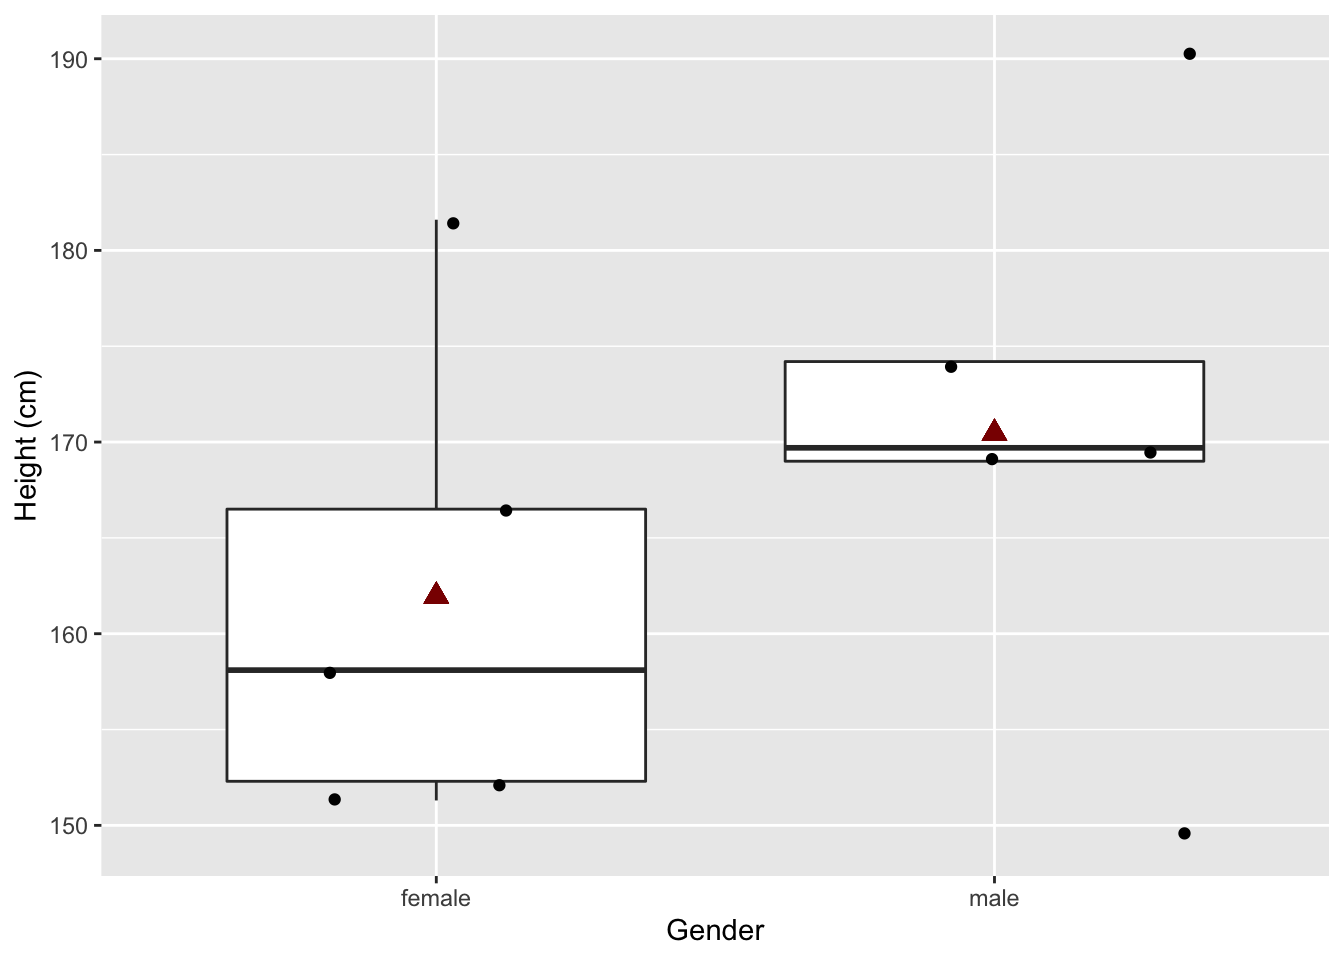
\includegraphics{Statistiek_2020_2021_files/figure-latex/unnamed-chunk-22-1.pdf}

\begin{Shaded}
\begin{Highlighting}[]
\NormalTok{res }\OperatorTok{\%\textgreater{}\%}\StringTok{ }\KeywordTok{ggplot}\NormalTok{(}\KeywordTok{aes}\NormalTok{(}\DataTypeTok{y =}\NormalTok{ verschil)) }\OperatorTok{+}\StringTok{ }\KeywordTok{geom\_boxplot}\NormalTok{() }\OperatorTok{+}\StringTok{ }
\StringTok{    }\KeywordTok{ylab}\NormalTok{(}\StringTok{"Gemiddeld Verschil (cm)"}\NormalTok{)}
\end{Highlighting}
\end{Shaded}

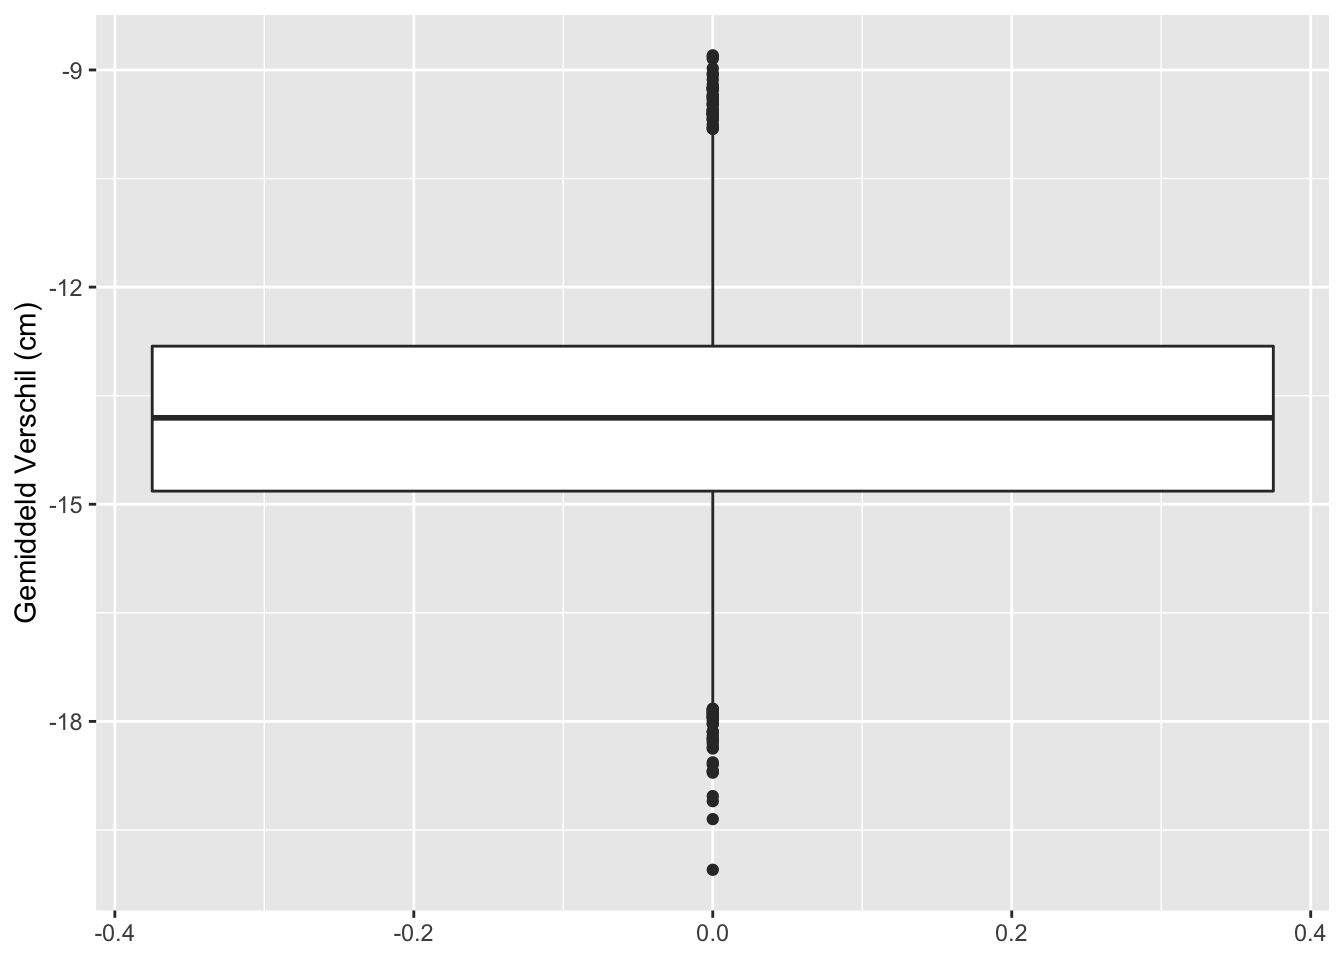
\includegraphics{Statistiek_2020_2021_files/figure-latex/unnamed-chunk-22-2.pdf}

\begin{Shaded}
\begin{Highlighting}[]
\KeywordTok{xlab}\NormalTok{(}\StringTok{""}\NormalTok{)}
\end{Highlighting}
\end{Shaded}

\begin{verbatim}
## $x
## [1] ""
## 
## attr(,"class")
## [1] "labels"
\end{verbatim}

\begin{itemize}
\item
  We zien dus dat we de kans om een verschil te vinden als er in werkelijkheid een verschil is in de populatie kunnen beïnvloeden in de design fase: aan de hand van de steekproefgrootte.
\item
  Hoe meer gegevens hoe makkelijker we het werkelijk verschil oppikken in de steekproef.
\item
  Dat wordt ook geïllustreerd in het gemiddelde verschil in lengte tussen mannen en vrouwen: daar zit in de grote studie veel minder variabiliteit op van steekproef tot steekproef omdat ze veel nauwkeuriger kunnen worden geschat omdat er meer gegevens zijn in de steekproef.
\end{itemize}

\hypertarget{controle-van-vals-positieven}{%
\subsubsection{Controle van vals positieven}\label{controle-van-vals-positieven}}

Wat gebeurt er als er geen verschil is tussen beide groepen?

\begin{itemize}
\item
  We moeten hiervoor experimenten simuleren waarbij de groepen gelijk zijn.
\item
  Hiervoor zullen we twee groepen vergelijken waarvoor de lengte gemiddeld niet verschillend is.
\item
  Dat kunnen we doen door een steekproef te trekken waarbij we voor beide groepen at random subjecten trekken uit de subset van vrouwen in de NHANES studie. Dan weten we dat er on de populatie geen verschil is in lengte tussen beide groepen die we zullen vergelijken.
\item
  Als we toch een verschil vinden in een steekproef dan weten we dat dit een vals positief resultaat is!
\item
  We doen de simulatiestudie opnieuw voor steekproeven met 5 subjecten per groep
\end{itemize}

\begin{Shaded}
\begin{Highlighting}[]
\KeywordTok{set.seed}\NormalTok{(}\DecValTok{13245}\NormalTok{)}
\CommentTok{\# Aantal simulaties en steekproefgrootte per groep}
\NormalTok{nSim \textless{}{-}}\StringTok{ }\DecValTok{10000}
\NormalTok{nSamp \textless{}{-}}\StringTok{ }\DecValTok{5}

\CommentTok{\# We filteren de data vooraf zodat we dit niet}
\CommentTok{\# telkens opnieuw hoeven te doen}
\NormalTok{fem \textless{}{-}}\StringTok{ }\NormalTok{nhanesSub }\OperatorTok{\%\textgreater{}\%}\StringTok{ }\KeywordTok{filter}\NormalTok{(Gender }\OperatorTok{==}\StringTok{ "female"}\NormalTok{)}

\CommentTok{\# Simulatie studie Om snelle functies te kunnen}
\CommentTok{\# gebruiken nemen we eerst nSim steekproeven en}
\CommentTok{\# berekenen we daarna alles.}

\NormalTok{femSamps \textless{}{-}}\StringTok{ }\NormalTok{femSamps2 \textless{}{-}}\StringTok{ }\KeywordTok{matrix}\NormalTok{(}\OtherTok{NA}\NormalTok{, }\DataTypeTok{nrow =}\NormalTok{ nSamp, }\DataTypeTok{ncol =}\NormalTok{ nSim)}
\ControlFlowTok{for}\NormalTok{ (i }\ControlFlowTok{in} \DecValTok{1}\OperatorTok{:}\NormalTok{nSim) \{}
\NormalTok{    femSamps[, i] \textless{}{-}}\StringTok{ }\KeywordTok{sample}\NormalTok{(fem}\OperatorTok{$}\NormalTok{Height, nSamp)}
\NormalTok{    femSamps2[, i] \textless{}{-}}\StringTok{ }\KeywordTok{sample}\NormalTok{(fem}\OperatorTok{$}\NormalTok{Height, nSamp)}
\NormalTok{\}}

\NormalTok{res \textless{}{-}}\StringTok{ }\KeywordTok{data.frame}\NormalTok{(}\DataTypeTok{verschil =} \KeywordTok{colMeans}\NormalTok{(femSamps) }\OperatorTok{{-}}\StringTok{ }\KeywordTok{colMeans}\NormalTok{(femSamps2), }
\NormalTok{    Rfast}\OperatorTok{::}\KeywordTok{ttests}\NormalTok{(femSamps, femSamps2))}

\KeywordTok{sum}\NormalTok{(res}\OperatorTok{$}\NormalTok{pvalue }\OperatorTok{\textless{}}\StringTok{ }\FloatTok{0.05} \OperatorTok{\&}\StringTok{ }\NormalTok{res}\OperatorTok{$}\NormalTok{verschil }\OperatorTok{\textless{}}\StringTok{ }\DecValTok{0}\NormalTok{)}
\end{Highlighting}
\end{Shaded}

\begin{verbatim}
## [1] 213
\end{verbatim}

\begin{Shaded}
\begin{Highlighting}[]
\KeywordTok{sum}\NormalTok{(res}\OperatorTok{$}\NormalTok{pvalue }\OperatorTok{\textgreater{}=}\StringTok{ }\FloatTok{0.05}\NormalTok{)}
\end{Highlighting}
\end{Shaded}

\begin{verbatim}
## [1] 9558
\end{verbatim}

\begin{Shaded}
\begin{Highlighting}[]
\KeywordTok{sum}\NormalTok{(res}\OperatorTok{$}\NormalTok{pvalue }\OperatorTok{\textless{}}\StringTok{ }\FloatTok{0.05} \OperatorTok{\&}\StringTok{ }\NormalTok{res}\OperatorTok{$}\NormalTok{verschil }\OperatorTok{\textgreater{}}\StringTok{ }\DecValTok{0}\NormalTok{)}
\end{Highlighting}
\end{Shaded}

\begin{verbatim}
## [1] 229
\end{verbatim}

\begin{Shaded}
\begin{Highlighting}[]
\NormalTok{res }\OperatorTok{\%\textgreater{}\%}\StringTok{ }\KeywordTok{ggplot}\NormalTok{(}\KeywordTok{aes}\NormalTok{(}\DataTypeTok{x =}\NormalTok{ verschil, }\DataTypeTok{y =} \OperatorTok{{-}}\KeywordTok{log10}\NormalTok{(pvalue), }
    \DataTypeTok{color =}\NormalTok{ pvalue }\OperatorTok{\textless{}}\StringTok{ }\FloatTok{0.05}\NormalTok{)) }\OperatorTok{+}\StringTok{ }\KeywordTok{geom\_point}\NormalTok{() }\OperatorTok{+}\StringTok{ }\KeywordTok{xlab}\NormalTok{(}\StringTok{"Gemiddeld Verschil (cm)"}\NormalTok{) }\OperatorTok{+}\StringTok{ }
\StringTok{    }\KeywordTok{ylab}\NormalTok{(}\StringTok{"Statistische Significantie ({-}log10 p)"}\NormalTok{)}
\end{Highlighting}
\end{Shaded}

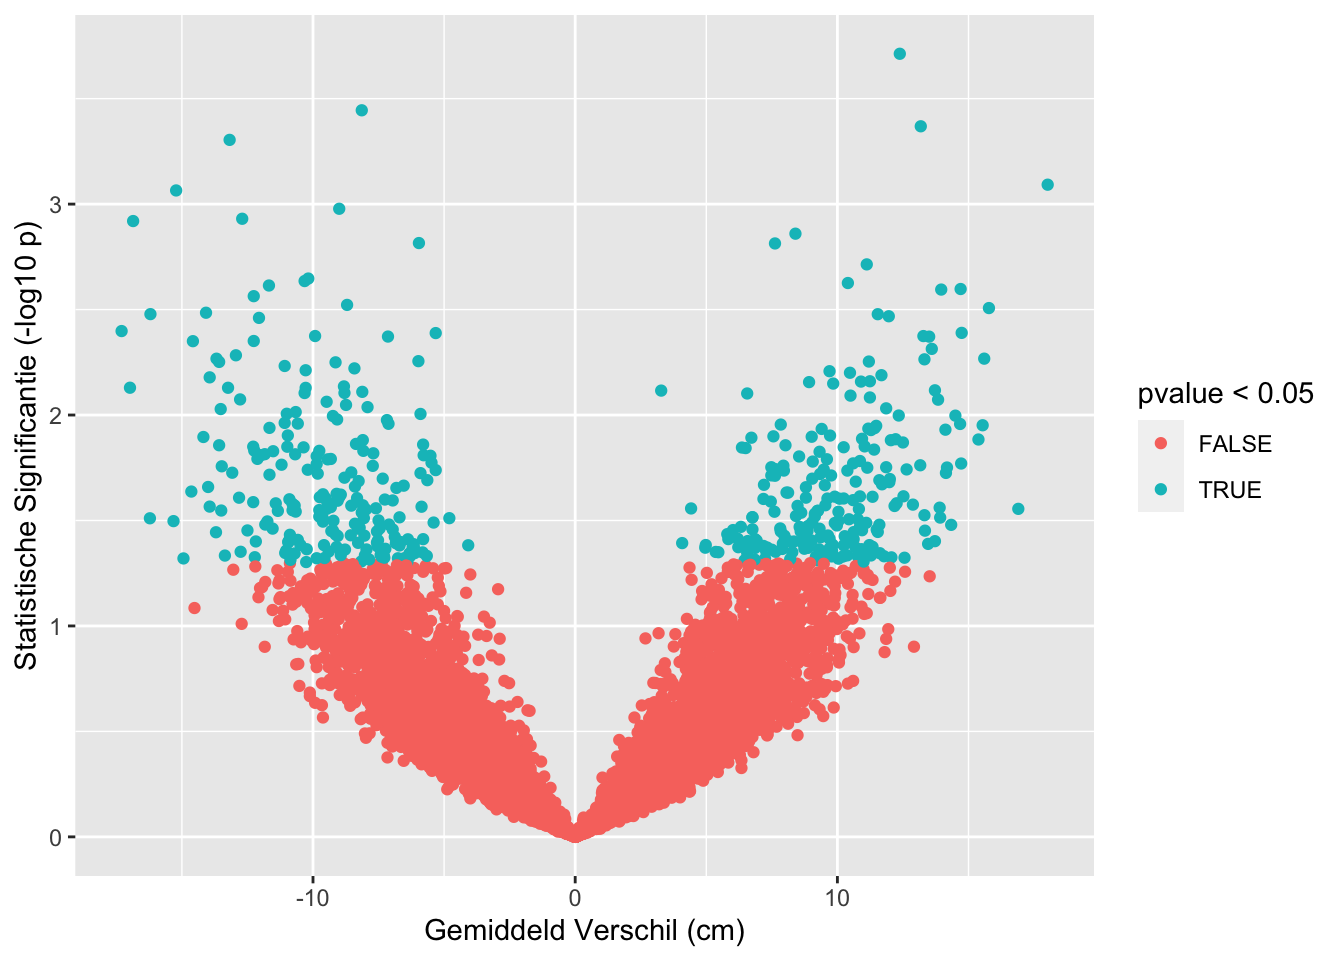
\includegraphics{Statistiek_2020_2021_files/figure-latex/unnamed-chunk-23-1.pdf}

\begin{Shaded}
\begin{Highlighting}[]
\NormalTok{res }\OperatorTok{\%\textgreater{}\%}\StringTok{ }\KeywordTok{ggplot}\NormalTok{(}\KeywordTok{aes}\NormalTok{(}\DataTypeTok{y =}\NormalTok{ verschil)) }\OperatorTok{+}\StringTok{ }\KeywordTok{geom\_boxplot}\NormalTok{() }\OperatorTok{+}\StringTok{ }
\StringTok{    }\KeywordTok{ylab}\NormalTok{(}\StringTok{"Gemiddeld Verschil (cm)"}\NormalTok{)}
\end{Highlighting}
\end{Shaded}

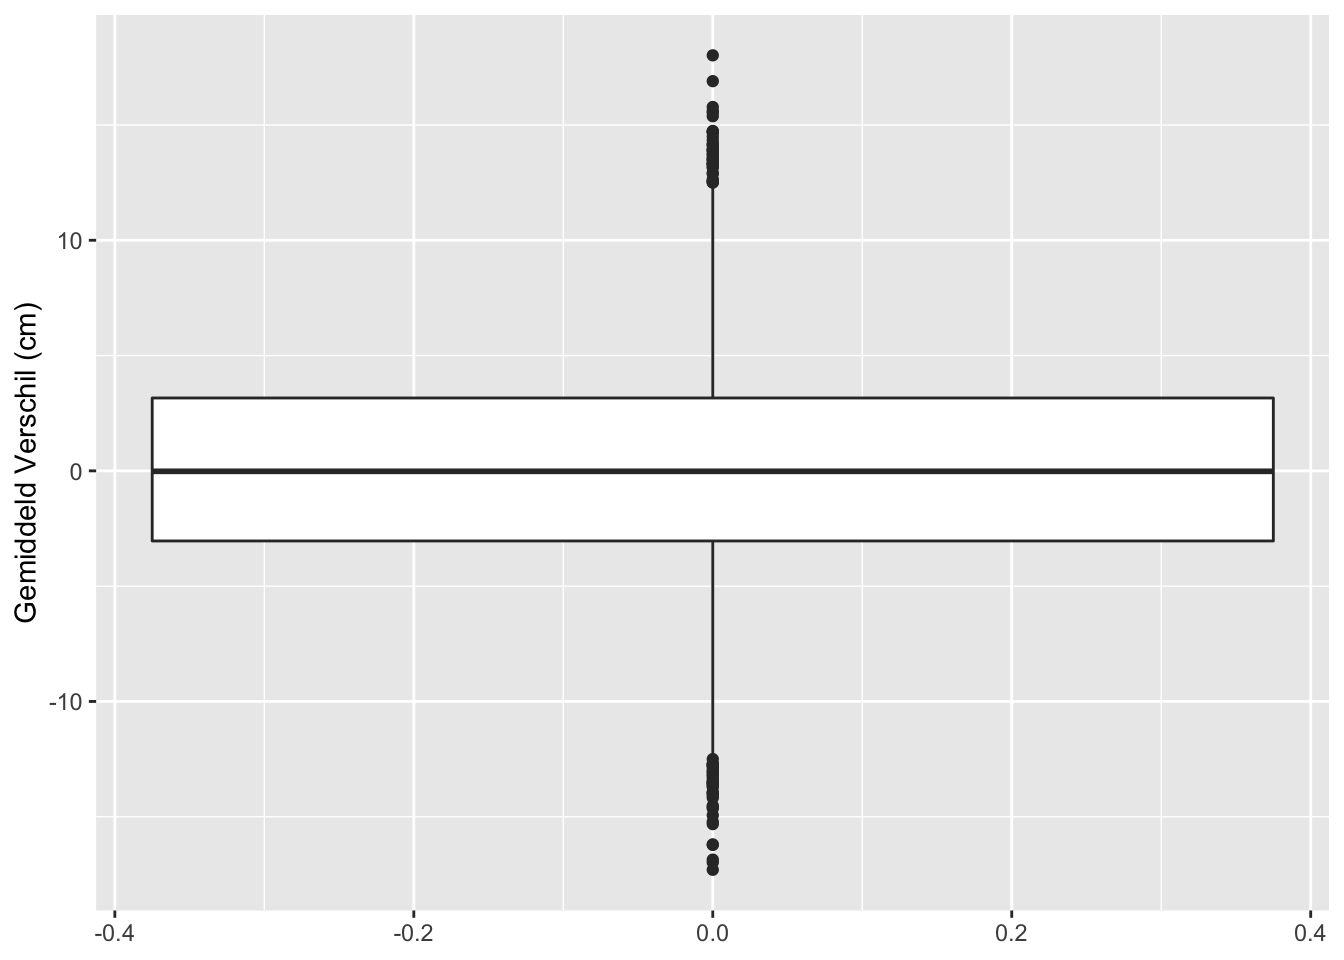
\includegraphics{Statistiek_2020_2021_files/figure-latex/unnamed-chunk-23-2.pdf}

\begin{Shaded}
\begin{Highlighting}[]
\KeywordTok{xlab}\NormalTok{(}\StringTok{""}\NormalTok{)}
\end{Highlighting}
\end{Shaded}

\begin{verbatim}
## $x
## [1] ""
## 
## attr(,"class")
## [1] "labels"
\end{verbatim}

Op basis van 10000 steekproeven zien we dat we in 442 steekproeven ten onrechte besluiten dat er een verschil is in gemiddelde lengte tussen twee groepen vrouwen.

Met de statistische analyse controleren we dus het aantal vals positieve resultaten correct op 5\%.

\emph{Wat gebeurt er als we het aantal observaties verhogen?}

We simuleren opnieuw experimenten met 50 subjecten per groep maar we trekken de subjecten opnieuw telkens uit de populatie van vrouwen.

\begin{Shaded}
\begin{Highlighting}[]
\KeywordTok{set.seed}\NormalTok{(}\DecValTok{1345}\NormalTok{)}
\CommentTok{\# Aantal simulaties en steekproefgrootte per groep}
\NormalTok{nSim \textless{}{-}}\StringTok{ }\DecValTok{10000}
\NormalTok{nSamp \textless{}{-}}\StringTok{ }\DecValTok{50}

\CommentTok{\# We filteren de data vooraf zodat we dit niet}
\CommentTok{\# telkens opnieuw hoeven te doen}
\NormalTok{fem \textless{}{-}}\StringTok{ }\NormalTok{nhanesSub }\OperatorTok{\%\textgreater{}\%}\StringTok{ }\KeywordTok{filter}\NormalTok{(Gender }\OperatorTok{==}\StringTok{ "female"}\NormalTok{)}

\CommentTok{\# Simulatie studie Om snelle functies te kunnen}
\CommentTok{\# gebruiken nemen we eerst nSim steekproeven en}
\CommentTok{\# berekenen we daarna alles.}

\NormalTok{femSamps \textless{}{-}}\StringTok{ }\NormalTok{femSamps2 \textless{}{-}}\StringTok{ }\KeywordTok{matrix}\NormalTok{(}\OtherTok{NA}\NormalTok{, }\DataTypeTok{nrow =}\NormalTok{ nSamp, }\DataTypeTok{ncol =}\NormalTok{ nSim)}
\ControlFlowTok{for}\NormalTok{ (i }\ControlFlowTok{in} \DecValTok{1}\OperatorTok{:}\NormalTok{nSim) \{}
\NormalTok{    femSamps[, i] \textless{}{-}}\StringTok{ }\KeywordTok{sample}\NormalTok{(fem}\OperatorTok{$}\NormalTok{Height, nSamp)}
\NormalTok{    femSamps2[, i] \textless{}{-}}\StringTok{ }\KeywordTok{sample}\NormalTok{(fem}\OperatorTok{$}\NormalTok{Height, nSamp)}
\NormalTok{\}}

\NormalTok{res \textless{}{-}}\StringTok{ }\KeywordTok{data.frame}\NormalTok{(}\DataTypeTok{verschil =} \KeywordTok{colMeans}\NormalTok{(femSamps) }\OperatorTok{{-}}\StringTok{ }\KeywordTok{colMeans}\NormalTok{(femSamps2), }
\NormalTok{    Rfast}\OperatorTok{::}\KeywordTok{ttests}\NormalTok{(femSamps, femSamps2))}

\KeywordTok{sum}\NormalTok{(res}\OperatorTok{$}\NormalTok{pvalue }\OperatorTok{\textless{}}\StringTok{ }\FloatTok{0.05} \OperatorTok{\&}\StringTok{ }\NormalTok{res}\OperatorTok{$}\NormalTok{verschil }\OperatorTok{\textless{}}\StringTok{ }\DecValTok{0}\NormalTok{)}
\end{Highlighting}
\end{Shaded}

\begin{verbatim}
## [1] 271
\end{verbatim}

\begin{Shaded}
\begin{Highlighting}[]
\KeywordTok{sum}\NormalTok{(res}\OperatorTok{$}\NormalTok{pvalue }\OperatorTok{\textgreater{}=}\StringTok{ }\FloatTok{0.05}\NormalTok{)}
\end{Highlighting}
\end{Shaded}

\begin{verbatim}
## [1] 9501
\end{verbatim}

\begin{Shaded}
\begin{Highlighting}[]
\KeywordTok{sum}\NormalTok{(res}\OperatorTok{$}\NormalTok{pvalue }\OperatorTok{\textless{}}\StringTok{ }\FloatTok{0.05} \OperatorTok{\&}\StringTok{ }\NormalTok{res}\OperatorTok{$}\NormalTok{verschil }\OperatorTok{\textgreater{}}\StringTok{ }\DecValTok{0}\NormalTok{)}
\end{Highlighting}
\end{Shaded}

\begin{verbatim}
## [1] 228
\end{verbatim}

\begin{Shaded}
\begin{Highlighting}[]
\NormalTok{res }\OperatorTok{\%\textgreater{}\%}\StringTok{ }\KeywordTok{ggplot}\NormalTok{(}\KeywordTok{aes}\NormalTok{(}\DataTypeTok{x =}\NormalTok{ verschil, }\DataTypeTok{y =} \OperatorTok{{-}}\KeywordTok{log10}\NormalTok{(pvalue), }
    \DataTypeTok{color =}\NormalTok{ pvalue }\OperatorTok{\textless{}}\StringTok{ }\FloatTok{0.05}\NormalTok{)) }\OperatorTok{+}\StringTok{ }\KeywordTok{geom\_point}\NormalTok{() }\OperatorTok{+}\StringTok{ }\KeywordTok{xlab}\NormalTok{(}\StringTok{"Gemiddeld Verschil (cm)"}\NormalTok{) }\OperatorTok{+}\StringTok{ }
\StringTok{    }\KeywordTok{ylab}\NormalTok{(}\StringTok{"Statistische Significantie ({-}log10 p)"}\NormalTok{)}
\end{Highlighting}
\end{Shaded}

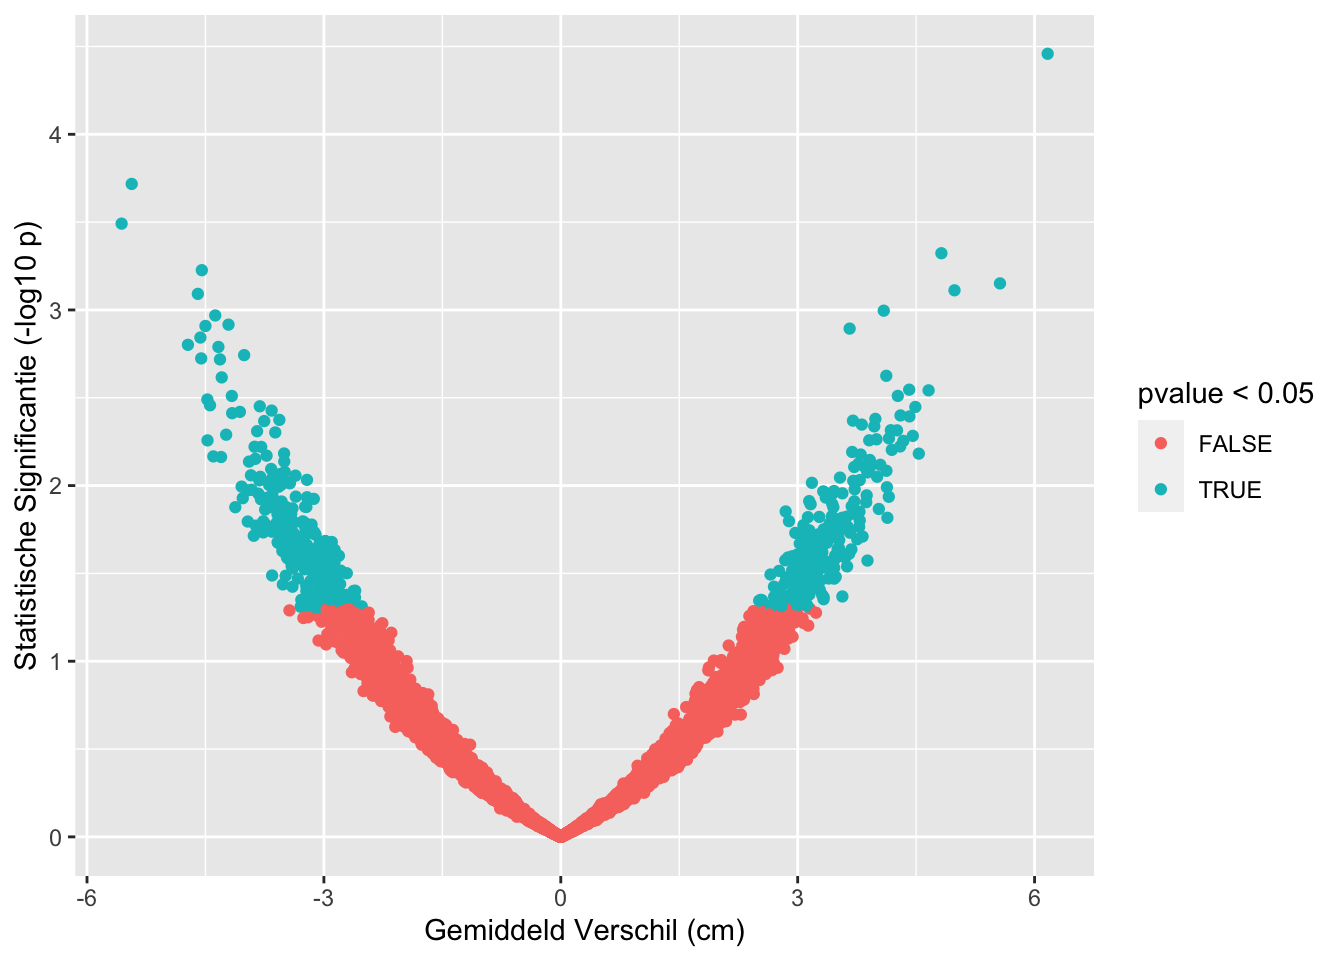
\includegraphics{Statistiek_2020_2021_files/figure-latex/unnamed-chunk-24-1.pdf}

\begin{Shaded}
\begin{Highlighting}[]
\NormalTok{res }\OperatorTok{\%\textgreater{}\%}\StringTok{ }\KeywordTok{ggplot}\NormalTok{(}\KeywordTok{aes}\NormalTok{(}\DataTypeTok{y =}\NormalTok{ verschil)) }\OperatorTok{+}\StringTok{ }\KeywordTok{geom\_boxplot}\NormalTok{() }\OperatorTok{+}\StringTok{ }
\StringTok{    }\KeywordTok{ylab}\NormalTok{(}\StringTok{"Gemiddeld Verschil (cm)"}\NormalTok{)}
\end{Highlighting}
\end{Shaded}

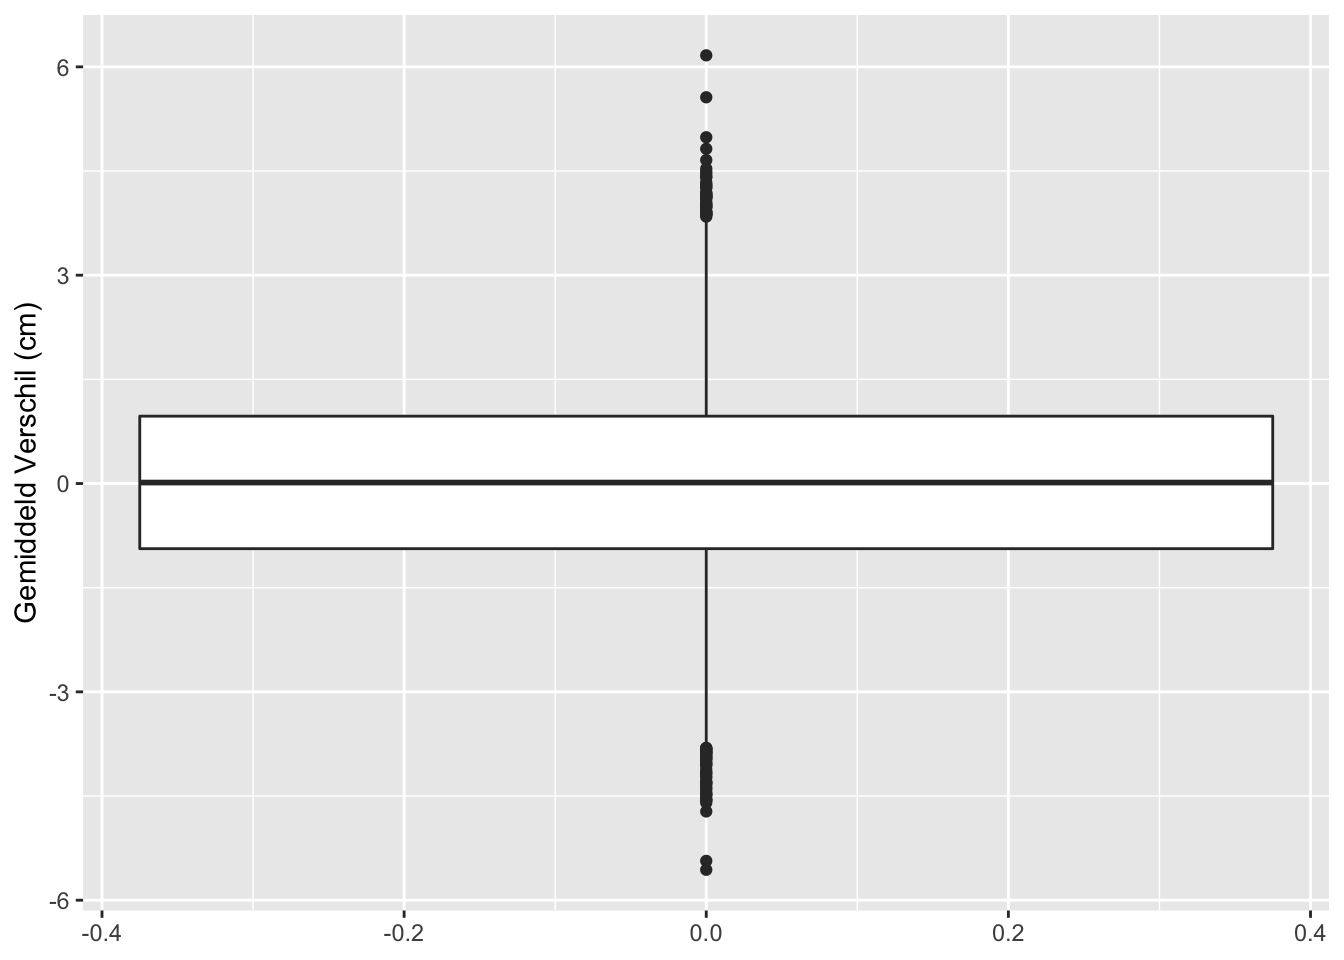
\includegraphics{Statistiek_2020_2021_files/figure-latex/unnamed-chunk-24-2.pdf}

\begin{Shaded}
\begin{Highlighting}[]
\KeywordTok{xlab}\NormalTok{(}\StringTok{""}\NormalTok{)}
\end{Highlighting}
\end{Shaded}

\begin{verbatim}
## $x
## [1] ""
## 
## attr(,"class")
## [1] "labels"
\end{verbatim}

Op basis van 10000 steekproeven zien we dat we in 499 steekproeven ten onrechte besluiten dat er een verschil is in gemiddelde lengte tussen twee groepen vrouwen.

Met de statistische analyse controleren we dus ook bij het nemen van een grote steekproef het aantal vals positieve resultaten correct op 5\%. (Vals positief: Op basis van de steekproef besluiten dat er gemiddeld een verschil is in lengte tussen beide groepen terwijl er in werkelijkheid geen verschil is in de populatie.)

\hypertarget{conclusies}{%
\subsection{Conclusies}\label{conclusies}}

\begin{enumerate}
\def\labelenumi{\arabic{enumi}.}
\item
  In elke steekproef worden at random andere proefpersonen uit de populatie getrokken.
\item
  Hierdoor verschillen lengte metingen van steekproef tot steekproef.
\item
  Dus ook het geschatte gemiddeldes en standaard deviaties.
\item
  Ook onze conclusies zijn onzeker en kunnen wijzigen van steekproef tot steekproef.
\item
  Met statistiek controleren we de kans op het trekken foute conclusies.
\end{enumerate}

\hypertarget{case-study-salk-vaccin}{%
\section{Case study: Salk vaccin}\label{case-study-salk-vaccin}}

In 1916, brak de eerste grote polio epidemie uit in de USA.
Begin de jaren 50 ontwikkelde John Salk een vaccin met belovende resultaten in het lab.
In 1954, heeft de National Foundation for Infantile Paralysis (NFIP) een grote studie opgezet om de effectiviteit van het Salk vaccin na te gaan.

\begin{itemize}
\tightlist
\item
  Veronderstel dat de NFIP in 1954 een groot aantal kinderen zou hebben gevaccineerd, wat zouden ze dan kunnen besluiten als de polio incidentie in 1954 lager was dan in 1953?
\end{itemize}

Neen, het zou gekund hebben dat het verschil in polio incidentie veroorzaakt werd door het feit dat de infectie minder hevig was in 1954.
We hebben dus een controle nodig!

\hypertarget{nfip-study}{%
\subsection{NFIP Study}\label{nfip-study}}

\hypertarget{design}{%
\subsubsection{Design}\label{design}}

\begin{itemize}
\tightlist
\item
  Grote simultane studie met gevaccineerde kinderen (cases) en ongevaccineerde kinderen (controles).
\item
  In scholen van districten met hoge polio incidentie.
\item
  Cases: kinderen van de tweede graad van het lager onderwijs waarvan de ouders toestemden met vaccinatie.
\item
  Controles: kinderen van de eerste en derde graad.
\end{itemize}

\hypertarget{data}{%
\subsubsection{Data}\label{data}}

\begin{Shaded}
\begin{Highlighting}[]
\NormalTok{nfip \textless{}{-}}\StringTok{ }\KeywordTok{tibble}\NormalTok{(}\DataTypeTok{group =} \KeywordTok{c}\NormalTok{(}\StringTok{"cases"}\NormalTok{, }\StringTok{"controls"}\NormalTok{, }\StringTok{"noConcent"}\NormalTok{), }
    \DataTypeTok{grade =} \KeywordTok{c}\NormalTok{(}\StringTok{"g2"}\NormalTok{, }\StringTok{"g1g3"}\NormalTok{, }\StringTok{"g2"}\NormalTok{), }\DataTypeTok{vaccin =} \KeywordTok{c}\NormalTok{(}\StringTok{"yes"}\NormalTok{, }
        \StringTok{"no"}\NormalTok{, }\StringTok{"no"}\NormalTok{), }\DataTypeTok{total =} \KeywordTok{c}\NormalTok{(}\DecValTok{221998}\NormalTok{, }\DecValTok{725173}\NormalTok{, }\DecValTok{123605}\NormalTok{), }
    \DataTypeTok{polio =} \KeywordTok{c}\NormalTok{(}\DecValTok{54}\NormalTok{, }\DecValTok{391}\NormalTok{, }\DecValTok{56}\NormalTok{)) }\OperatorTok{\%\textgreater{}\%}\StringTok{ }\KeywordTok{mutate}\NormalTok{(}\DataTypeTok{noPolio =}\NormalTok{ total }\OperatorTok{{-}}\StringTok{ }
\StringTok{    }\NormalTok{polio)}
\NormalTok{knitr}\OperatorTok{::}\KeywordTok{kable}\NormalTok{(nfip, }\StringTok{"html"}\NormalTok{)}
\end{Highlighting}
\end{Shaded}

group

grade

vaccin

total

polio

noPolio

cases

g2

yes

221998

54

221944

controls

g1g3

no

725173

391

724782

noConcent

g2

no

123605

56

123549

We zien 54 polio besmettingen bij de gevaccineerde kinderen
en 391 bij de controle groep.

\begin{itemize}
\tightlist
\item
  Kunnen we daaruit besluiten trekken?
\end{itemize}

De twee groepen verschillen echter ook in grootte!

We zullen daarom kijken naar polio incidentie per miljoen kinderen.

\begin{enumerate}
\def\labelenumi{\arabic{enumi}.}
\tightlist
\item
  We voegen een extra column toe aan het nfip data object d.m.v. de mutate functie. We berekenen de incidentie per miljoen kinderen (incidencePM) en slaan de gewijzigde dataset op onder dezelfde naam.
\item
  we maken de tabel opnieuw
\end{enumerate}

\begin{Shaded}
\begin{Highlighting}[]
\NormalTok{nfip \textless{}{-}}\StringTok{ }\NormalTok{nfip }\OperatorTok{\%\textgreater{}\%}\StringTok{ }\KeywordTok{mutate}\NormalTok{(}\DataTypeTok{incidencePM =} \KeywordTok{round}\NormalTok{(nfip}\OperatorTok{$}\NormalTok{polio}\OperatorTok{/}\NormalTok{nfip}\OperatorTok{$}\NormalTok{total }\OperatorTok{*}\StringTok{ }
\StringTok{    }\FloatTok{1e+06}\NormalTok{, }\DecValTok{0}\NormalTok{))}
\NormalTok{knitr}\OperatorTok{::}\KeywordTok{kable}\NormalTok{(nfip, }\StringTok{"html"}\NormalTok{)}
\end{Highlighting}
\end{Shaded}

group

grade

vaccin

total

polio

noPolio

incidencePM

cases

g2

yes

221998

54

221944

243

controls

g1g3

no

725173

391

724782

539

noConcent

g2

no

123605

56

123549

453

\begin{itemize}
\item
  We observeren nu dat de incidentie meer dan dubbel zo hoog is in de controle groep als in de vaccinatie groep.
\item
  We observeren echter ook dat de incidentie lager is in de groep van kinderen uit de tweede graad waarvan de ouders geen toestemming gaven voor inenting!?
\item
  Wat betekent dit?
\end{itemize}

\hypertarget{confounding}{%
\subsection{Confounding}\label{confounding}}

\begin{center}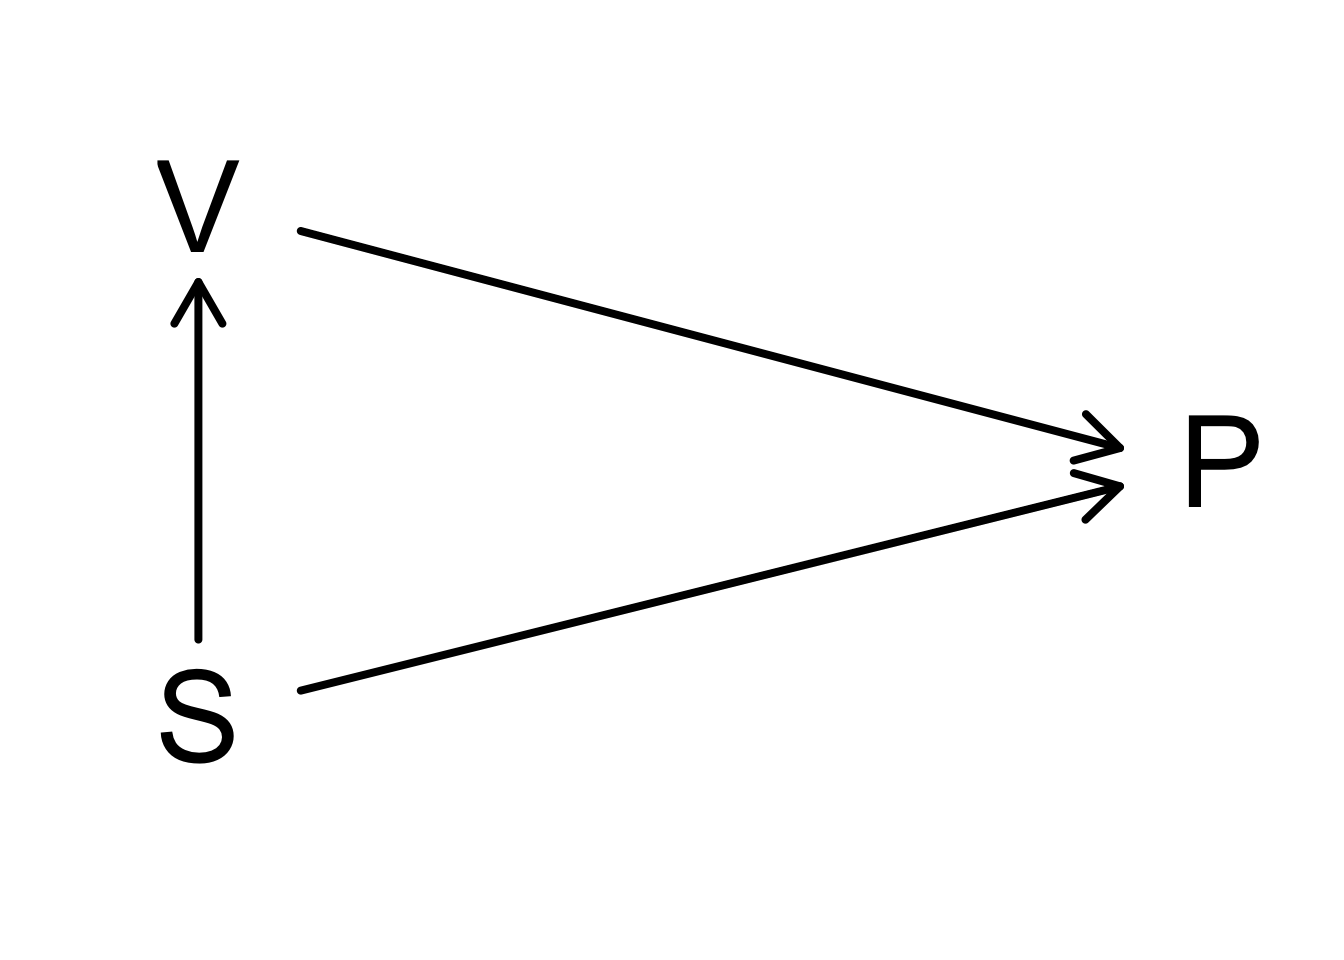
\includegraphics[width=0.5\linewidth]{Statistiek_2020_2021_files/figure-latex/unnamed-chunk-27-1} \end{center}

We observeren een lagere polio (P) incidentie voor kinderen bij wie de ouders geen toestemming gaven dan in de controle groep.
Toestemming voor vaccinatie (V) is geassocieerd met de socio-economische status (S).
Kinderen van lagere socio-economische status zijn meer resistent tegen de ziekte.

Er is dus sprake van confounding: de socio-economische status is geassocieerd met zowel de polio incidentie als met de toestemming op vaccinatie.

Controle groep en gevaccineerde groep zijn dus niet vergelijkbaar:
Ze verschillen in socio economische status en bovendien ook in leeftijd!
We kunnen aan de hand van het experiment het effect van de vaccinatie niet correct inschatten.

\hypertarget{salk-study}{%
\subsection{Salk Study}\label{salk-study}}

\hypertarget{design-1}{%
\subsubsection{Design}\label{design-1}}

Een nieuwe studie werd uitgevoerd: dubbel blinde gerandomiseerde studie.

\begin{itemize}
\tightlist
\item
  Kinderen worden at random toegewezen aan controle of case arm van het experiment nadat de ouders toestemden met vaccinatie.
\item
  Controle: vaccinatie met placebo
\item
  Treatment: vaccinatie met vaccin
\item
  Double blinding:

  \begin{itemize}
  \tightlist
  \item
    ouders en kinderen weten niet of ze werden gevaccineerd of niet
  \item
    medische staf en onderzoekers weten niet of het kind het vaccin of de placebo kreeg
  \end{itemize}
\end{itemize}

\hypertarget{data-1}{%
\subsubsection{Data}\label{data-1}}

\begin{Shaded}
\begin{Highlighting}[]
\NormalTok{salk \textless{}{-}}\StringTok{ }\KeywordTok{data.frame}\NormalTok{(}\DataTypeTok{group =} \KeywordTok{c}\NormalTok{(}\StringTok{"cases"}\NormalTok{, }\StringTok{"control"}\NormalTok{, }\StringTok{"noConcent"}\NormalTok{), }
    \DataTypeTok{treatment =} \KeywordTok{c}\NormalTok{(}\StringTok{"vaccine"}\NormalTok{, }\StringTok{"placebo"}\NormalTok{, }\StringTok{"none"}\NormalTok{), }\DataTypeTok{total =} \KeywordTok{c}\NormalTok{(}\DecValTok{200745}\NormalTok{, }
        \DecValTok{201229}\NormalTok{, }\DecValTok{338778}\NormalTok{), }\DataTypeTok{polio =} \KeywordTok{c}\NormalTok{(}\DecValTok{57}\NormalTok{, }\DecValTok{142}\NormalTok{, }\DecValTok{157}\NormalTok{)) }\OperatorTok{\%\textgreater{}\%}\StringTok{ }
\StringTok{    }\KeywordTok{mutate}\NormalTok{(}\DataTypeTok{noPolio =}\NormalTok{ total }\OperatorTok{{-}}\StringTok{ }\NormalTok{polio, }\DataTypeTok{incidencePM =} \KeywordTok{round}\NormalTok{(polio}\OperatorTok{/}\NormalTok{total }\OperatorTok{*}\StringTok{ }
\StringTok{        }\FloatTok{1e+06}\NormalTok{, }\DecValTok{0}\NormalTok{))}
\NormalTok{knitr}\OperatorTok{::}\KeywordTok{kable}\NormalTok{(salk, }\StringTok{"html"}\NormalTok{)}
\end{Highlighting}
\end{Shaded}

group

treatment

total

polio

noPolio

incidencePM

cases

vaccine

200745

57

200688

284

control

placebo

201229

142

201087

706

noConcent

none

338778

157

338621

463

\begin{itemize}
\item
  We observeren een veel groter effect nu dat cases en controles vergelijkbaar zijn, incidentie van respectievelijk 284 and 706 per miljoen.
\item
  De polio incidentie voor kinderen die geen toestemming geven blijft vergelijkbaar 453 and 463 per miljoen respectievelijk in the NFIP and Salk study.
\end{itemize}

We zullen later in de cursus tonen dat het effect van het vaccin statistisch significant is.

\hypertarget{rol-van-statistiek}{%
\section{Rol van Statistiek}\label{rol-van-statistiek}}

In deze introductie hebben we gezien dat statistiek een belangrijke rol speelt in empirisch onderzoek. We toonden aan dat

\begin{enumerate}
\def\labelenumi{\arabic{enumi}.}
\item
  \emph{Proefopzet} is essentieel

  \begin{itemize}
  \item
    het belangrijk is om de scope van de studie goed te specifiëren voor de start van het experiment
  \item
    randomisatie nodig is om een representatieve steekproef te nemen
  \item
    steekproef grootte is heel belangrijk
  \item
    we moeten ons bewust zijn van Confounding
  \item
    een goede controle is belangrijk
  \end{itemize}
\item
  \emph{Data exploratie en beschrijvende statistiek}:

  \begin{itemize}
  \tightlist
  \item
    exploreren
  \item
    visualiseren
  \item
    samenvatten en beschrijven van geobserveerde data zodat relevante aspecten naar voor komen.
  \end{itemize}
\item
  \emph{Statistische besluitvorming}: aan de hand van statistische modellen bestuderen in hoeverre geobserveerde trends/effecten die geobserveerd worden in een steekproef veralgemeend kunnen worden naar de algemene populatie.
\end{enumerate}

\hypertarget{belangrijke-concepten-conventies}{%
\chapter{Belangrijke concepten \& conventies}\label{belangrijke-concepten-conventies}}

Alle kennisclips die in dit hoofdstuk zijn verwerkt kan je in deze youtube playlist vinden: \href{https://www.youtube.com/playlist?list=PLZH1hP8_LbJJ7apU5sAbRlUsve2nWz5ev}{Kennisclips Hoofdstuk2}

\hypertarget{inleiding}{%
\section{Inleiding}\label{inleiding}}

De verschillende stappen in een studie worden geïllustreerd in
Figuur \ref{fig:pop2Samp2Pop}.
Eerst bepaalt de onderzoeker de \emph{populatie} van interesse.
Gezien het om financiële en logistieke beperkingen vrijwel nooit mogelijk is om de volledige populatie te onderzoeken zal men vervolgens een steekproef nemen uit de populatie.
De manier waarop een steekproef zal worden genomen wordt vastgelegd in het \emph{design van de studie}.
\emph{Proefopzet} of \emph{studie design} is een aparte tak van de statisitiek en is een cruciaal onderdeel van een studie.
Het studie design moet immers garanderen dat de gegevens en resultaten van de steekproef representatief zijn voor de populatie zodat de resultaten van de studie veralgemeneend kunnen worden naar de populatie toe.
Vervolgens wordt de studie uitgevoerd, worden de gegevens verzameld en kan de eigenlijke data-analyse van start gaan.
In een eerste fase is het belangrijk om de gegevens grondig te exploreren.
\emph{Data-exploratie en beschrijvende statistiek} is een tweede tak van de statistiek die toelaat om gegevens van de steekproef te visualiseren, samen te vatten en om inzicht in de data te verwerven.
Dat is belangrijk om de data correct te kunnen modelleren en om aannames na te kunnen gaan die nodig zijn voor de verdere data analyse. Vervolgens zullen we hetgeen we observeren in de steekproef trachten te veralgemenen naar de algemene populatie toe, zodat we algemene conclusies kunnen trekken op populatie-niveau op basis van de steekproef van de studie. Hiervoor zijn methodes nodig van de \emph{statistische besluitvorming}, ook wel \emph{statistische inferentie} genoemd, een derde belangrijke tak van de statistiek.

\begin{figure}

{\centering 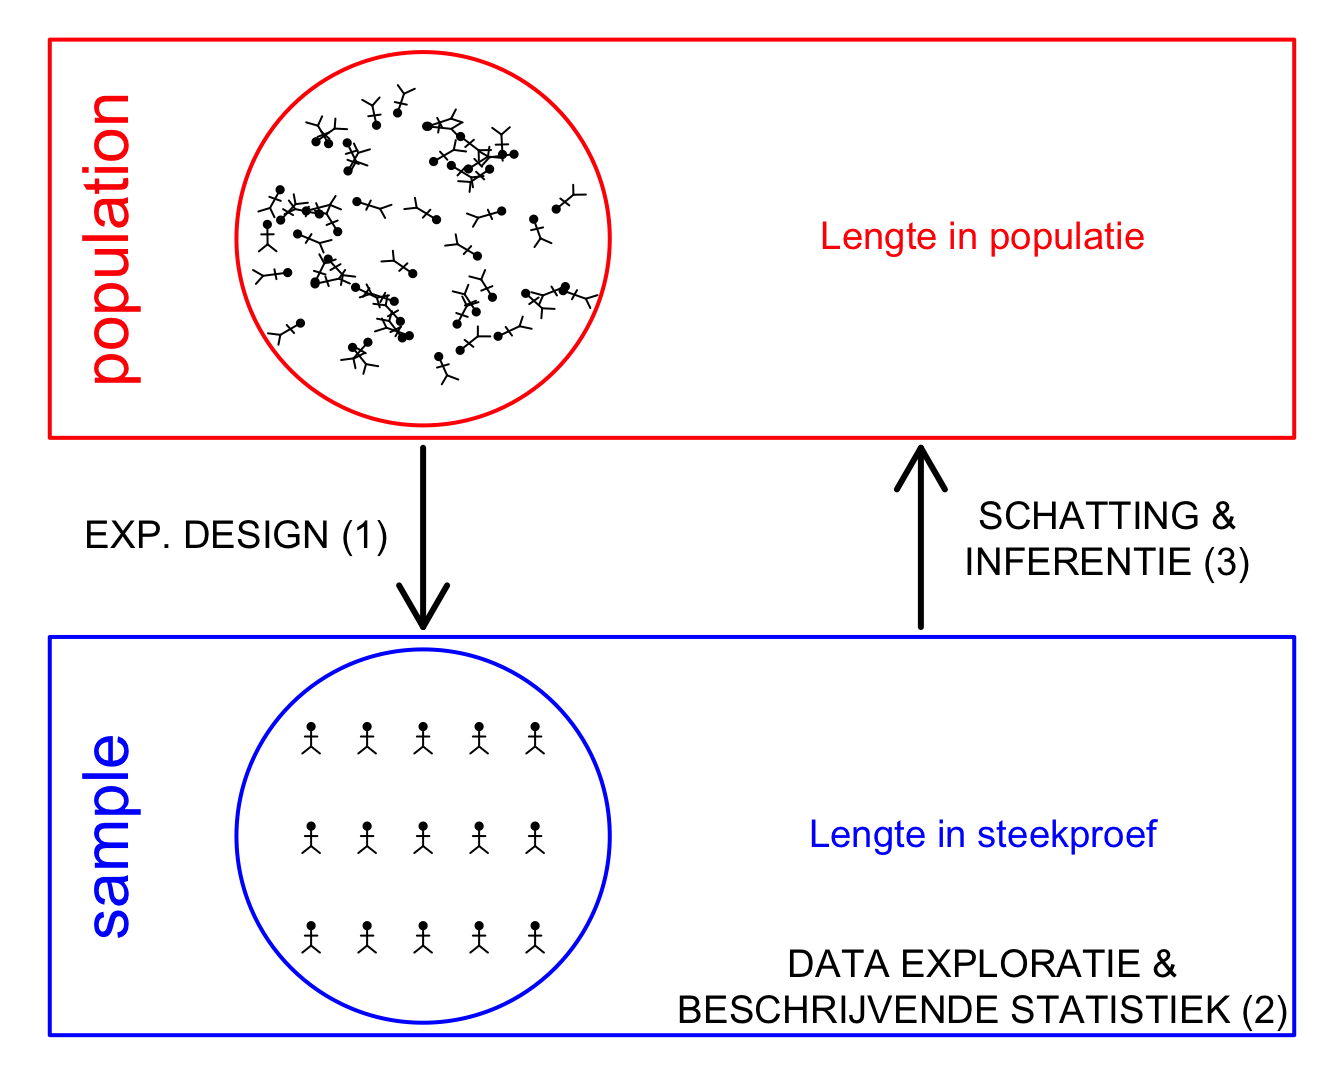
\includegraphics[width=1\linewidth]{Statistiek_2020_2021_files/figure-latex/pop2Samp2Pop-1} 

}

\caption{Verschillende stappen in een studie. (1) In de design fase/ proefopzet definieert de onderzoeker de populatie, bepaalt hij/zij op welke manier een steekproef zal worden genomen uit de populatie en hoe het experiment zal worden uitgevoerd. Ook het volledige data analyse plan moet in deze fase zijn vastgelegd. Vervolgens wordt het experiment uitgevoerd en worden de gegevens verzameld. (2) De gegevens worden vervolgens verkend en samengevat. Hierbij verwerft men inzicht in de gegevens en kunnen aannames worden nagegaan die noodzakelijk zijn voor de verdere data analyse stappen. (3) Tenslotte zal men hetgeen men observeert in de steekproef trachten te veralgemenen naar de populatie toe a.d.h.v. statistische inferentie.}\label{fig:pop2Samp2Pop}
\end{figure}

Vooraleer we dieper ingaan op studie-design, data-exploratie en statistische besluitvorming zullen we eerst enkele concepten introduceren.
We doen dat in dit hoofdstuk aan de hand van de de NHANES studie.

\begin{example}[NHANES studie]
\begin{example}

\protect\hypertarget{exm:nhanesExConcepten}{}{\label{exm:nhanesExConcepten} \iffalse (NHANES studie) \fi{} }

\end{example}
\end{example}

De National Health and Nutrition Examination Survey
(NHANES) wordt sinds 1960 op regelmatige basis afgenomen. In dit voorbeeld maken we gebruik van de gegevens die werden verzameld tussen 2009-2012 bij 10000 Amerikanen en die werden opgenomen in het R-pakket NHANES. Er werd een groot aantal fysieke, demografische, nutritionele, levelsstijl en gezondheidskarakteristieken gecollecteerd in deze studie (zie Tabel \ref{tab:nhanesConcepten}).

\textbf{Einde voorbeeld}

\begin{table}[t]

\caption{\label{tab:nhanesConcepten}Overzicht van een aantal variabelen uit de NHANES studie.}
\centering
\begin{tabular}{rlrlrr}
\toprule
ID & Gender & Height & BMI\_WHO & DirectChol & SexNumPartnLife\\
\midrule
51624 & male & 164.7 & 30.0\_plus & 1.29 & 8\\
51625 & male & 105.4 & 12.0\_18.5 & NA & NA\\
51630 & female & 168.4 & 30.0\_plus & 1.16 & 10\\
51638 & male & 133.1 & 12.0\_18.5 & 1.34 & NA\\
51646 & male & 130.6 & 18.5\_to\_24.9 & 1.55 & NA\\
\addlinespace
51647 & female & 166.7 & 25.0\_to\_29.9 & 2.12 & 20\\
\bottomrule
\end{tabular}
\end{table}

\hypertarget{variabelen}{%
\section{Variabelen}\label{variabelen}}

\begin{table}[t]

\caption{\label{tab:nhanesConcepten2}Overzicht van een aantal variabelen uit de NHANES studie.}
\centering
\begin{tabular}{rlrlrr}
\toprule
ID & Gender & Height & BMI\_WHO & DirectChol & SexNumPartnLife\\
\midrule
51624 & male & 164.7 & 30.0\_plus & 1.29 & 8\\
51625 & male & 105.4 & 12.0\_18.5 & NA & NA\\
51630 & female & 168.4 & 30.0\_plus & 1.16 & 10\\
51638 & male & 133.1 & 12.0\_18.5 & 1.34 & NA\\
51646 & male & 130.6 & 18.5\_to\_24.9 & 1.55 & NA\\
\addlinespace
51647 & female & 166.7 & 25.0\_to\_29.9 & 2.12 & 20\\
\bottomrule
\end{tabular}
\end{table}

Een \emph{variabele} is een karakteristiek (bvb. Systolische bloeddruk, leeftijd, geslacht, \ldots)
die varieert van subject tot subject (bvb. van persoon tot persoon, van dier tot dier, \ldots) in de studie.
Er zijn verschillende \emph{types} variabelen.

\emph{Kwalitatieve variabelen} hebben (meestal) beperkt aantal
uitkomstcategorieën die niet numeriek van aard zijn. Deze worden
onderverdeeld in \emph{nominale variabelen} en \emph{ordinale variabelen}
. Nominale gegevens zijn er die men kan benoemen. Ze worden niet gemeten en kennen geen natuurlijke ordening; bijvoorbeeld geslacht, ras,
bloedgroep, kleur van ogen, \ldots{}
Ordinale variabelen kennen wel een ordening; bijvoorbeeld de BMI klasse volgens het WHO, de rokersstatus (nooit gerookt, ooit gerookt maar
gestopt, actueel roker), \ldots{}

Een ander type van variabelen zijn \emph{numerieke variabelen}. Hierbij maakt men het onderscheid tussen \emph{numerieke discrete variabelen} en \emph{numerieke continue variabelen}.
Numerieke discrete variabelen bestaan uit tellingen, b.v. het aantal partners die men had gedurende het leven (geregistreerd in de NHANES studie), het aantal salamanders van de species \textbf{P. jordani} in een bepaald gebied, het aantal reads dat mapt op een bepaald gen in een genexpressiestudie waarbij men gebruik maakt van next-generation sequencing technologie , \ldots{}

Numerieke continue variabelen kunnen (tenminste in theorie) tussen bepaalde grenzen elke mogelijke waarde aannemen. Bijvoorbeeld, leeftijd is continu want het verschil in leeftijd tussen 2 personen kan in principe willekeurig klein zijn (1 uur, 1 minuut, \ldots). Analoog zijn het gewicht, BMI, fluorescentie-metingen in een ELISA experiment, \ldots{} continue metingen.

In de wetenschappen gaat men vaak continue
gegevens dichotomiseren om ze nominaal te maken. Bijvoorbeeld, systolische
bloeddruk wordt omgezet in hypertensie (\(>140\) mmHg) en normotensie (\(\leq 140\)
mmHg). Dit vereenvoudigt de beschrijving van gegevens. Helaas is dit een
slechte praktijk omdat het meestal leidt tot een aanzienlijk verlies aan informatie en
omdat de aldus bekomen resultaten sterk afhankelijk kunnen zijn van de
gekozen drempelwaarde. In de praktijk worden de uitkomsten van continue
variabelen ook vaak afgerond zodat de vermelde waarden in feite discreet
zijn. Om analoge redenen is het vaak wenselijk om ze als continue variabelen
te blijven beschouwen.

In de praktijk wil men vaak numerieke rangen toekennen aan de verschillende
waarden die ordinale variabelen aannemen. Bijvoorbeeld kan men ervoor kiezen
de codes 1, 2 en 3 toe te kennen aan de meetwaarden \emph{nooit gerookt}, \emph{ooit gerookt maar gestopt} en \emph{actueel roker}.
Het is belangrijk om te beseffen dat de keuze van die numerieke waarden vaak geen betekenis heeft.
Het verschil tussen de toegekende codes (3-2=1, 2-1=1, 3-2=1) is niet bruikbaar gezien men bijvoorbeeld niet onderstellen dat de wijziging in rokerstatus identiek is van \emph{nooit gerookt} naar \emph{ooit gerookt maar gestopt} (2-1=1) en van \emph{ooit gerookt maar gestopt} naar \emph{actueel roker} (3-2=1).

\begin{example}[oefening]
\begin{example}

\protect\hypertarget{exm:unnamed-chunk-30}{}{\label{exm:unnamed-chunk-30} \iffalse (oefening) \fi{} }

\end{example}
\end{example}

Geef het type aan van de variabelen in Tabel \ref{tab:nhanesConcepten}

\hypertarget{subsec:pop}{%
\section{Populatie}\label{subsec:pop}}

Het doel van een wetenschappelijke studie is nagenoeg altijd om uitspraken te doen over de algemene populatie.
Stel bijvoorbeeld dat men een grenswaarde wil afleiden om patiënten met hypertensie op te sporen.
Hiervoor zal men eerst de systolische bloeddruk moeten bestuderen bij een populatie van gezonde personen.
Een populatie is meestal continu in verandering.
Bovendien is men meestal niet alleen geïnteresseerd in effecten bij huidige subjecten, maar ook in het effect bij toekomstige subjecten.
De populatie kan dus als oneindig groot worden beschouwd en is op een bepaald ogenblik zelfs niet volledig observeerbaar\footnote{B.v. omdat het ook toekomstige subjecten omvat}.
De populatie kan binnen de statistiek dus worden opgevat als een theoretisch concept die alle huidige en toekomstige subjecten omvat waarover men uitspraken wenst te doen.
In de praktijk zal men dus nooit de volledige populatie kunnen bemonsteren en dient men een steekproef te nemen van de populatie.
Om een representatieve groep subjecten te waarborgen, vertrekt een goede onderzoeksopzet vanuit een belangrijke, precies geformuleerde vraagstelling
omtrent een duidelijk omschreven populatie.
Vaak worden hierbij inclusie- en exclusiecriteria geformuleerd.

\emph{Inclusiecriteria} zijn karakteristieken die een subject/experimentele eenheid moet hebben om tot de populatie te behoren, b.v.

\begin{itemize}
\tightlist
\item
  specifieke ziekte: hypertensie
\item
  leeftijdscategorie
\item
  geslacht
\item
  \ldots{}
\end{itemize}

\emph{Exclusiecriteria} zijn karakteristieken die een subject/experimentele eenheid niet mag hebben om tot de populatie te behoren, b.v.

\begin{itemize}
\tightlist
\item
  geneesmiddelen gebruik
\item
  andere ziekten
\item
  zwangerschap
\item
  \ldots{}
\end{itemize}

Op de subjecten zal men meestal een aantal karakteristieken meten, ook wel \emph{variabelen} genoemd (bvb. Systolische bloeddruk, leeftijd, geslacht, \ldots). Typisch zullen deze variabelen variëren van subject tot subject (bvb. van persoon tot persoon, van dier tot dier, \ldots) in de populatie.

\hypertarget{toevalsveranderlijken-of-toevallige-veranderlijken}{%
\section{Toevalsveranderlijken (of toevallige veranderlijken)}\label{toevalsveranderlijken-of-toevallige-veranderlijken}}

De belangrijke vraag, waar we in in de verdere hoofdstukken dieper op in
zullen gaan, is hoe nauwkeurig we uitspraken kunnen doen over de populatie o.b.v. een groep gemeten subjecten in een steekproef.
De spreiding op de gegevens zal daar een cruciale rol in spelen.
Als de gegevens niet variëren tussen subjecten, dan zullen alle steekproeven uit de populatie hetzelfde resultaat opleveren en zullen de bekomen schattingen niet afwijken van de gezochte populatieparameters.
Als daarentegen de gegevens zeer chaotisch zijn, dan zullen verschillende steekproeven mogelijks zeer verschillende resultaten opleveren, die bijgevolg ver kunnen afwijken van de gezochte populatieparameters.

Om het denkwerk te vergemakkelijken, zullen we hoofdletters gebruiken om aan te geven dat
de bestudeerde karakteristiek (vb. een meetresultaat zoals systolische bloeddruk) variabel is in de populatie,
zonder daarbij concreet over de gerealiseerde waarde
voor een bepaald subject na te denken.
Dergelijke meting of variabele \(X\) wordt
algemeen een \emph{toevalsveranderlijke} of \emph{toevallige veranderlijke} genoemd, (a) omdat ze formeel het
resultaat aanduidt van een \emph{toevallige trekking} van een bepaalde
karakteristiek uit de studiepopulatie en (b) omdat ze bovendien \emph{veranderlijk} is,
niet alle subjecten in de steekproef bezitten immers dezelfde waarde
voor die karakteristiek.

Het makkelijkst om over een toevalsveranderlijke \(X\) na te denken is alsof \(X\) het label voorstelt van
een bepaalde populatiekarakteristiek voor een lukraak individu uit de
bestudeerde populatie, vooraleer haar concrete waarde gemeten werd.
Met andere woorden, een toevalsveranderlijke \(X\) kan men opvatten als onbekende veranderlijke die een meting voorstelt die we plannen te verzamelen, maar nog niet hebben verzameld.
Net zoals observaties kunnen we toevallig veranderlijken klasseren als kwalitatief, kwantitatief, discreet, continu, \ldots.

\hypertarget{beschrijven-van-de-populatie}{%
\section{Beschrijven van de populatie}\label{beschrijven-van-de-populatie}}

Voor we een random variabele meten, kunnen we onmogelijk zeggen hoe hoog de meting precies zal zijn.
De gerealiseerde waarde van \(X\) is dus onderhevig aan random variabiliteit.
De geobserveerde steekproef in de NHANES studie \(x_1, x_2, . . . , x_{10000}\) kan dus als n = 10000 realisaties worden beschouwd van dezelfde random variable X, voor subject \(i\), met \(i = 1,2,...,10000\).
Een random veranderlijke, een karakteristiek van de populatie, wordt beschreven door gebruik te maken van een \emph{verdeling}.

De verdeling beschrijft de waarschijnlijkheid om een bepaalde waarde te observeren voor de toevallig veranderlijke wanneer men volledige lukraak een proefpersoon kiest uit de populatie.

Als we weten hoe de variabele verdeeld is dan kunnen we probabiliteitstheorie gebruiken om de kans te berekenen dat een bepaald voorval (event) zich voordoet: vb wat is de kans dat het IQ van een random subject uit de populatie kleiner of gelijk is aan 80.

\begin{itemize}
\item
  Notatie:

  \begin{itemize}
  \tightlist
  \item
    Event: \(X \leq 80\)
  \item
    Probabiliteit op event: \(Pr(X \leq 80)\)
  \end{itemize}
\end{itemize}

\hypertarget{intermezzo-probabiliteitstheorie}{%
\subsection{Intermezzo probabiliteitstheorie}\label{intermezzo-probabiliteitstheorie}}

\hypertarget{discrete-toevallig-veranderlijken}{%
\subsubsection{Discrete toevallig veranderlijken}\label{discrete-toevallig-veranderlijken}}

Stel dat we een discrete random variabele meten \(X\). Alle mogelijke waarden voor \(X\) worden de steekproefruimte \(\Omega\) genoemd.

\begin{itemize}
\item
  Voor Gender is de steekproefruimte \(\Omega=(0,1)\) met 0 (vrouw) or 1 (man).
\item
  Voor het werpen van een dobbelsteen is de steekproefruimte \(\Omega=(1,2,3,4,5,6)\).
\end{itemize}

Een event \(A\) is een subset van de steekproefruimte

\begin{itemize}
\tightlist
\item
  Een even getal werpen met een dobbelsteen: \(A=(2,4,6)\).
\item
  Kan ook een specifieke waarde zijn \(A=(1)\).
\end{itemize}

Event ruimte \(\mathcal{A}\) is de klasse van alle mogelijke events die kunnen optreden bij een bepaald experiment.

Twee events (\(A_1\) en \(A_2\)) zijn multueel exclusief als ze niet samen op kunnen treden.

\begin{itemize}
\tightlist
\item
  v.b. event van de oneven getallen \(A_1=(1,3,5)\) en het event om \(A_2=(6)\) te gooien.
\item
  Dus \(A_1 \bigcap A_2=\emptyset\).
\end{itemize}

Probabiliteit \(Pr(A)\) is een function \(Pr: A \rightarrow [0,1]\) die voldoet aan

\begin{enumerate}
\def\labelenumi{\arabic{enumi}.}
\tightlist
\item
  \(Pr(A) \geq 0\) en \(Pr(A) \leq 1\) voor elke \(A \in \mathcal{A}\)
\item
  \(Pr(\Omega)=1\)
\item
  Voor multueel exclusieve events \(A_1, A_2, \ldots A_k\) geldt dat \(Pr(A_1 \cup A_2 \ldots \cup A_k)= Pr(A_1) + \ldots + Pr(A_k)\)
\end{enumerate}

Dobbelsteen voorbeeld

\begin{itemize}
\tightlist
\item
  oneven number \(A=(1,3,5)\): is de unie van 3 multueel exclusieve events \(A_1=1\), \(A_2=3\) en \(A_3=5\) zodat
  \(Pr(A)=Pr(1)+Pr(3)+Pr(5)=1/6+1/6+1/6=0.5\)
\item
  \(\Omega=(1,2,3,4,5,6)\): \(Pr(\Omega)=1\)
\end{itemize}

Als we twee subjecten (j en k) onafhankelijk trekken van de populatie dan is de gezamelijke probabiliteit
\(P(X_j,X_k)= P(X_j)P(X_j)\)

\hypertarget{distributie-of-verdeling}{%
\paragraph{Distributie of verdeling}\label{distributie-of-verdeling}}

De distributie of de verdeling van een discrete toevallig veranderlijke \(X\) beschrijft de kans op elke mogelijke waarde van de steekproefruimte.

Voorbeeld: Gender is een binaire variabele (0: vrouw, 1: man) en binaire variabelen volgen een Bernoulli verdeling. 50.8\% van de subjecten in de Amerikaanse populatie zijn vrouw en 49.2\% is man.

Laat \(\pi\) de probabiliteit zijn op een man \(\pi=0.492\).
\[ X\sim \left \{
    \begin{array}{lcl}
    P(X=0) &=& 1-\pi\\
    P(X=1) &=& \pi
    \end{array} \right . \]

\begin{Shaded}
\begin{Highlighting}[]
\KeywordTok{tibble}\NormalTok{(}\DataTypeTok{X =} \KeywordTok{c}\NormalTok{(}\DecValTok{0}\NormalTok{, }\DecValTok{1}\NormalTok{), }\DataTypeTok{prob =} \KeywordTok{c}\NormalTok{(}\FloatTok{0.508}\NormalTok{, }\FloatTok{0.492}\NormalTok{)) }\OperatorTok{\%\textgreater{}\%}\StringTok{ }\KeywordTok{ggplot}\NormalTok{(}\KeywordTok{aes}\NormalTok{(}\DataTypeTok{x =}\NormalTok{ X, }
    \DataTypeTok{xend =}\NormalTok{ X, }\DataTypeTok{y =} \DecValTok{0}\NormalTok{, }\DataTypeTok{yend =}\NormalTok{ prob)) }\OperatorTok{+}\StringTok{ }\KeywordTok{geom\_segment}\NormalTok{() }\OperatorTok{+}\StringTok{ }
\StringTok{    }\KeywordTok{ylab}\NormalTok{(}\StringTok{"Probability"}\NormalTok{)}
\end{Highlighting}
\end{Shaded}

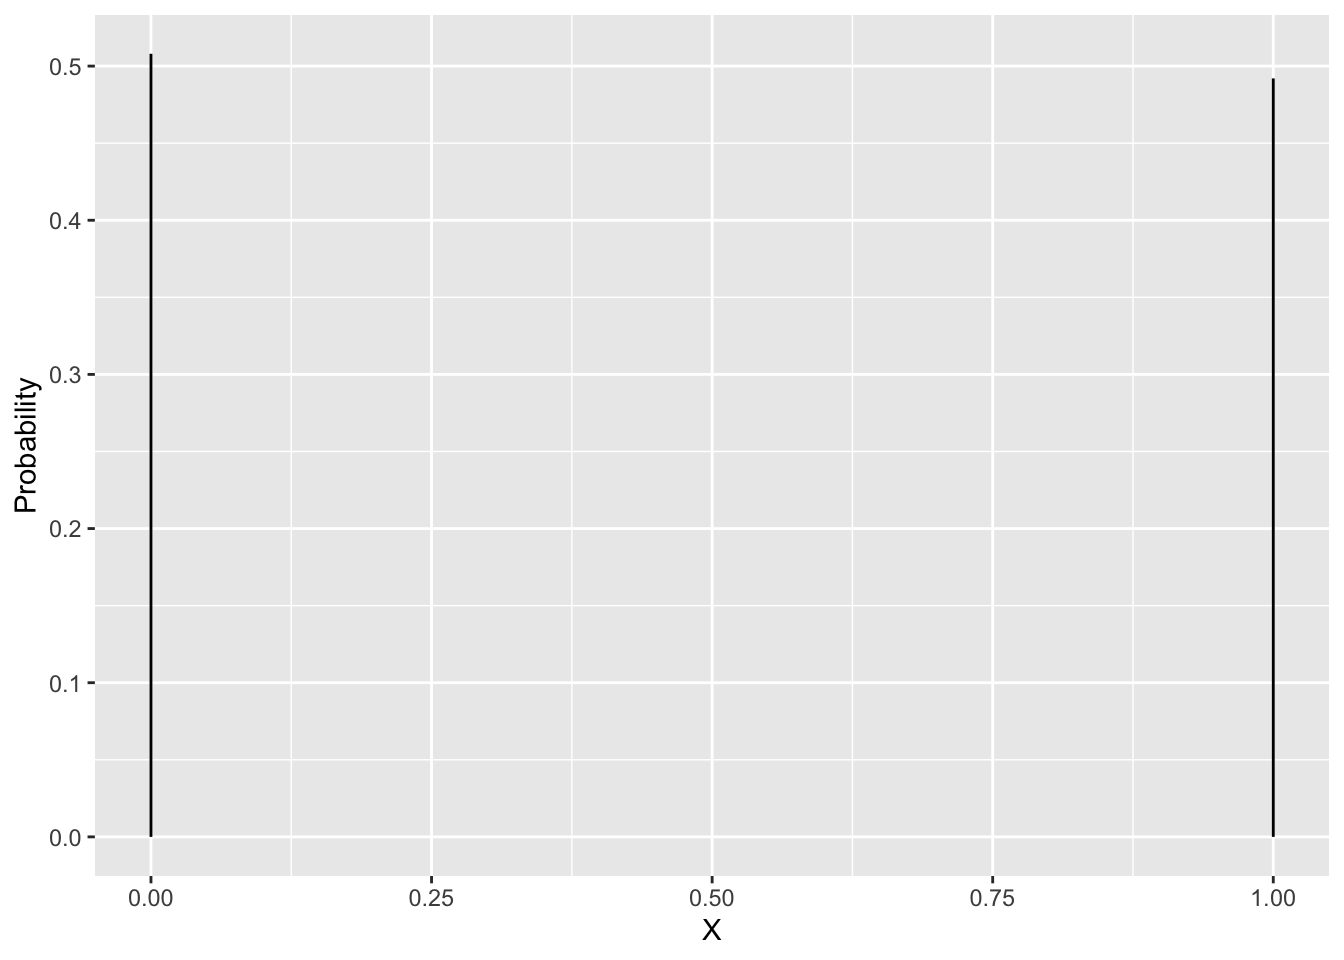
\includegraphics{Statistiek_2020_2021_files/figure-latex/unnamed-chunk-31-1.pdf}

Toevallig veranderlijke \(X\) volgt een Bernoulli verdeling \(B(\pi)\) met parameter \(\pi=0.492\),
\[B(\pi)= \pi^x(1-\pi)^{(x-1)}\]

\hypertarget{cumulative-distributie-functie}{%
\paragraph{Cumulative distributie functie}\label{cumulative-distributie-functie}}

De cumulative distributie functie F(x) geeft de probabiliteit weer om een random variable X te observeren waarvoor geldt dat \(X\leq x\):
\[ F(x) = \sum\limits_{\forall X\leq x} P(x)\]

Gender voorbeeld \(F(0)=1-\pi\) and \(F(1)= P(X=0) + P(X=1)=1\)

\begin{Shaded}
\begin{Highlighting}[]
\KeywordTok{tibble}\NormalTok{(}\DataTypeTok{X =} \KeywordTok{c}\NormalTok{(}\DecValTok{0}\NormalTok{, }\DecValTok{1}\NormalTok{), }\DataTypeTok{cumprob =} \KeywordTok{c}\NormalTok{(}\FloatTok{0.508}\NormalTok{, }\DecValTok{1}\NormalTok{)) }\OperatorTok{\%\textgreater{}\%}\StringTok{ }\KeywordTok{ggplot}\NormalTok{(}\KeywordTok{aes}\NormalTok{(}\DataTypeTok{x =}\NormalTok{ X, }
    \DataTypeTok{xend =}\NormalTok{ X, }\DataTypeTok{y =} \DecValTok{0}\NormalTok{, }\DataTypeTok{yend =}\NormalTok{ cumprob)) }\OperatorTok{+}\StringTok{ }\KeywordTok{geom\_segment}\NormalTok{() }\OperatorTok{+}\StringTok{ }
\StringTok{    }\KeywordTok{ylab}\NormalTok{(}\StringTok{"F(x)"}\NormalTok{)}
\end{Highlighting}
\end{Shaded}

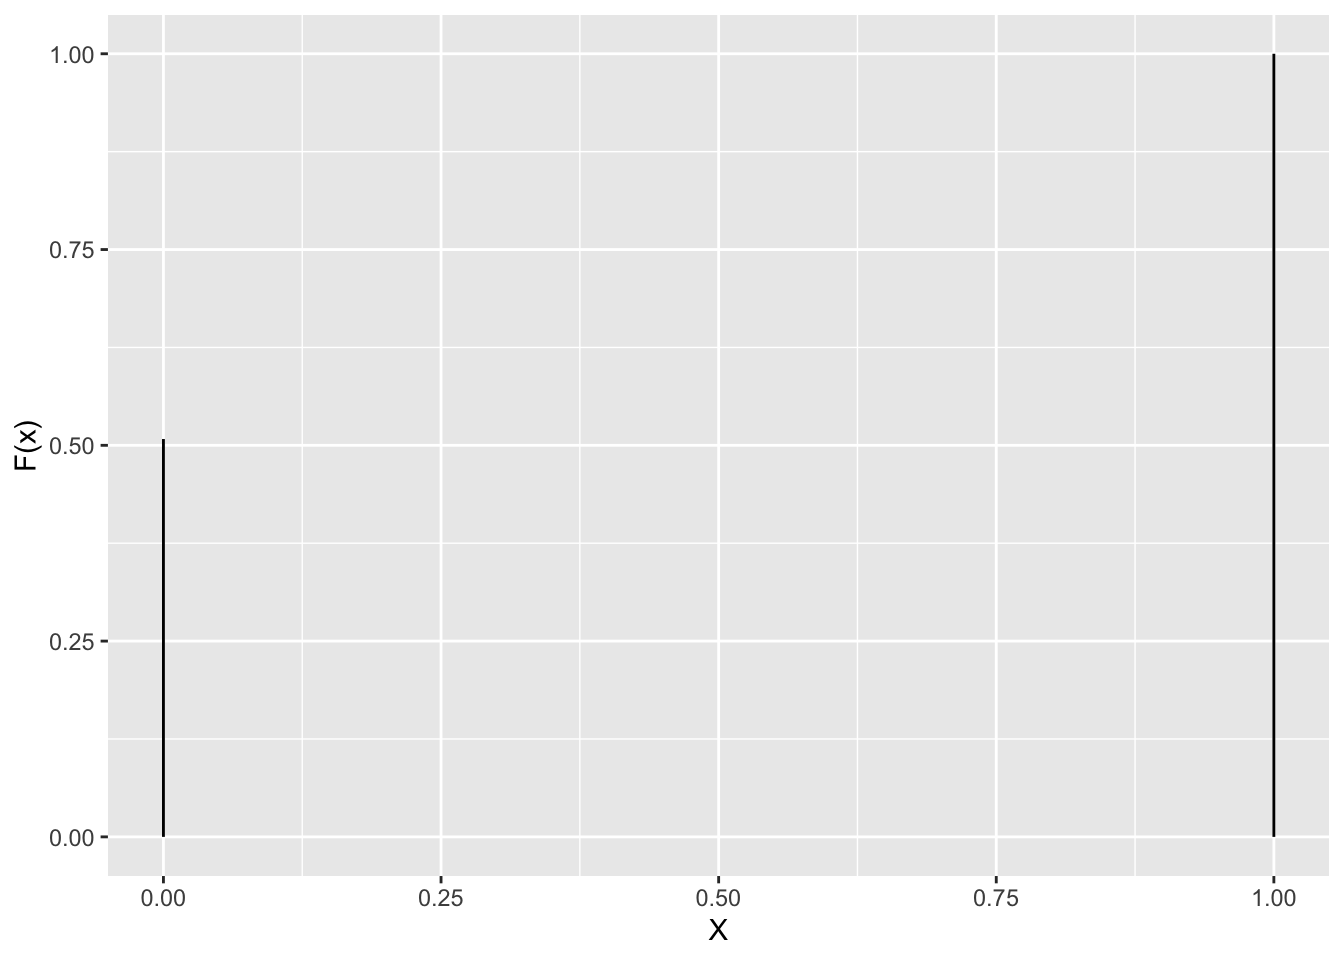
\includegraphics{Statistiek_2020_2021_files/figure-latex/unnamed-chunk-32-1.pdf}

Dobbelsteen voorbeeld:

\begin{Shaded}
\begin{Highlighting}[]
\KeywordTok{tibble}\NormalTok{(}\DataTypeTok{X =} \DecValTok{1}\OperatorTok{:}\DecValTok{6}\NormalTok{, }\DataTypeTok{cumprob =} \KeywordTok{cumsum}\NormalTok{(}\KeywordTok{rep}\NormalTok{(}\DecValTok{1}\OperatorTok{/}\DecValTok{6}\NormalTok{, }\DecValTok{6}\NormalTok{))) }\OperatorTok{\%\textgreater{}\%}\StringTok{ }
\StringTok{    }\KeywordTok{ggplot}\NormalTok{(}\KeywordTok{aes}\NormalTok{(}\DataTypeTok{x =}\NormalTok{ X, }\DataTypeTok{xend =}\NormalTok{ X, }\DataTypeTok{y =} \KeywordTok{rep}\NormalTok{(}\DecValTok{0}\NormalTok{, }\DecValTok{6}\NormalTok{), }\DataTypeTok{yend =}\NormalTok{ cumprob)) }\OperatorTok{+}\StringTok{ }
\StringTok{    }\KeywordTok{geom\_segment}\NormalTok{() }\OperatorTok{+}\StringTok{ }\KeywordTok{ylab}\NormalTok{(}\StringTok{"F(x)"}\NormalTok{)}
\end{Highlighting}
\end{Shaded}

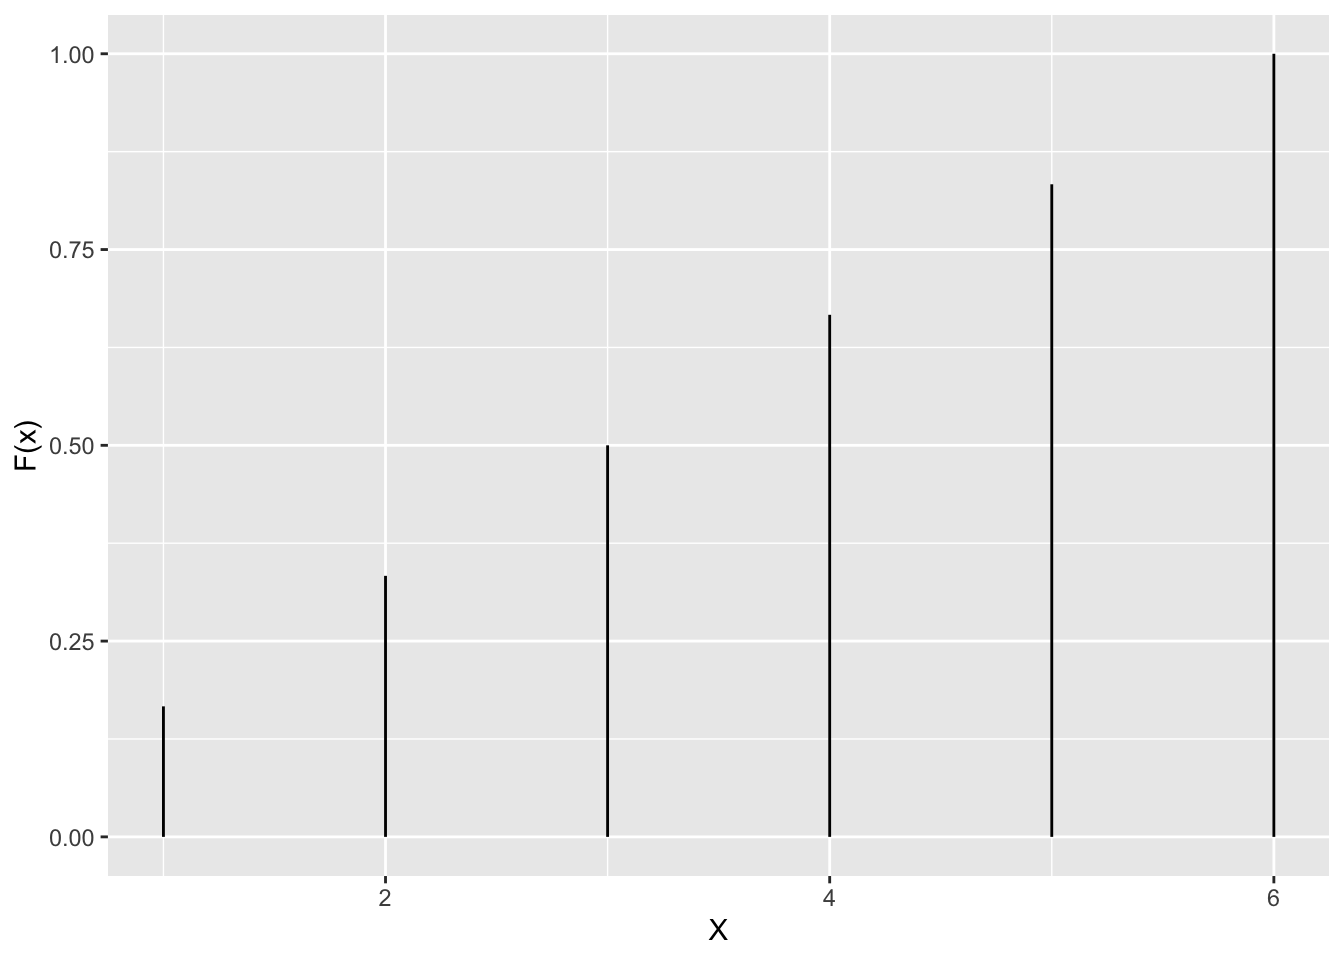
\includegraphics{Statistiek_2020_2021_files/figure-latex/unnamed-chunk-33-1.pdf}

\hypertarget{gemiddelde}{%
\paragraph{Gemiddelde}\label{gemiddelde}}

Het gemiddelde of de verwachte waarde \(E[X]\) van een discrete toevallig veranderlijke \(X\) is gegeven door:

\[E[X]=\sum\limits_{x\in\Omega} x P(X=x)\]

Merk op dat de operator \[E[.]\] staat voor de verwachte waarde van een toevallige veranderlijke of een functie van toevallig veranderlijken.

Gender voorbeeld

\[E[X]= 0 \times (1-\pi) + 1 \times (\pi) = \pi\]

Het gemiddelde is \(E[X]=0.492\).

Dobbelsteen voorbeeld

\(E[X]= 1 \times \frac{1}{6} + 2 \times \frac{1}{6} + \ldots + 6 \times \frac{1}{6} =\) 3.5

\hypertarget{variantie}{%
\paragraph{Variantie}\label{variantie}}

De variantie is een maat voor de variabiliteit van een toevallig veranderlijke en wordt gegeven door:

\[E[(X-E[X])^2]=\sum\limits_{x\in\Omega} (x-E[X])^2 P(X=x)\]

Het is dus de verwachte waarde van de kwadratische afwijkingen van een toevallig veranderlijke rond zijn gemiddelde en is dus een maat voor de variabiliteit of spreiding van de toevallige veranderlijke.

Gender voorbeeld
\begin{eqnarray}
    E[(X-E[X])^2]&=&(0-\pi)^2\times (1-\pi)+(1-\pi)^2 \times \pi\\
    &=& \pi^2 (1-\pi) + (1-\pi)^2 \pi\\
    &=&\pi (1-\pi)(\pi+1-\pi)\\
    &=&\pi(1-\pi)
    \end{eqnarray}

\hypertarget{continue-toevallig-veranderlijke}{%
\subsubsection{Continue toevallig veranderlijke}\label{continue-toevallig-veranderlijke}}

Een continue toevallig veranderlijke kan binnen bepaalde grenzen alle mogelijke waarden aannemen. De kans dat een continue toevallige veranderlijke exact één bepaalde waarde aan te nemen is daarom gelijk aan 0.

De distributie (verdeling) wordt daarom weergegeven a.d.h.v. de densiteitsfunctie of de dichtheidsfunctie \(f(x)\)

Veel biologische karakteristieken zijn approximatief normaal verdeeld (lengte, bloeddruk, IQ, concentratie metingen na logaritmische transformatie)

\[f(x) = \frac{1}{\sqrt{2\pi\sigma^2}} e^{-\frac{(x-\mu)^2}{2\sigma^2}}\]

Dat wordt kort genoteerd als

\[f(x) = N(\mu,\sigma^2)\]

Van het IQ is geweten dat het normale verdeling volgt met gemiddelde \(\mu=100\) en standaardafwijking \(\sigma=15\).

\[IQ \sim N(100,15^2)\]

In R kunnen we de dnorm functie gebruiken om de densiteit te berekenen voor een bepaalde waarde X=x.

\begin{itemize}
\tightlist
\item
  De argumenten van \texttt{dnorm} zijn \texttt{mean} (\(\mu\)) en \texttt{sd} (standaardafwijking \(\sigma\)).
\end{itemize}

\begin{Shaded}
\begin{Highlighting}[]
\NormalTok{iq \textless{}{-}}\StringTok{ }\KeywordTok{tibble}\NormalTok{(}\DataTypeTok{IQ =} \KeywordTok{seq}\NormalTok{(}\DecValTok{40}\NormalTok{, }\DecValTok{150}\NormalTok{, }\FloatTok{0.1}\NormalTok{), }\DataTypeTok{Densiteit =} \KeywordTok{dnorm}\NormalTok{(}\KeywordTok{seq}\NormalTok{(}\DecValTok{40}\NormalTok{, }
    \DecValTok{150}\NormalTok{, }\FloatTok{0.1}\NormalTok{), }\DataTypeTok{mean =} \DecValTok{100}\NormalTok{, }\DataTypeTok{sd =} \DecValTok{15}\NormalTok{))}
\NormalTok{iq }\OperatorTok{\%\textgreater{}\%}\StringTok{ }\KeywordTok{ggplot}\NormalTok{(}\KeywordTok{aes}\NormalTok{(}\DataTypeTok{x =}\NormalTok{ IQ, }\DataTypeTok{y =}\NormalTok{ Densiteit)) }\OperatorTok{+}\StringTok{ }\KeywordTok{geom\_line}\NormalTok{()}
\end{Highlighting}
\end{Shaded}

\begin{center}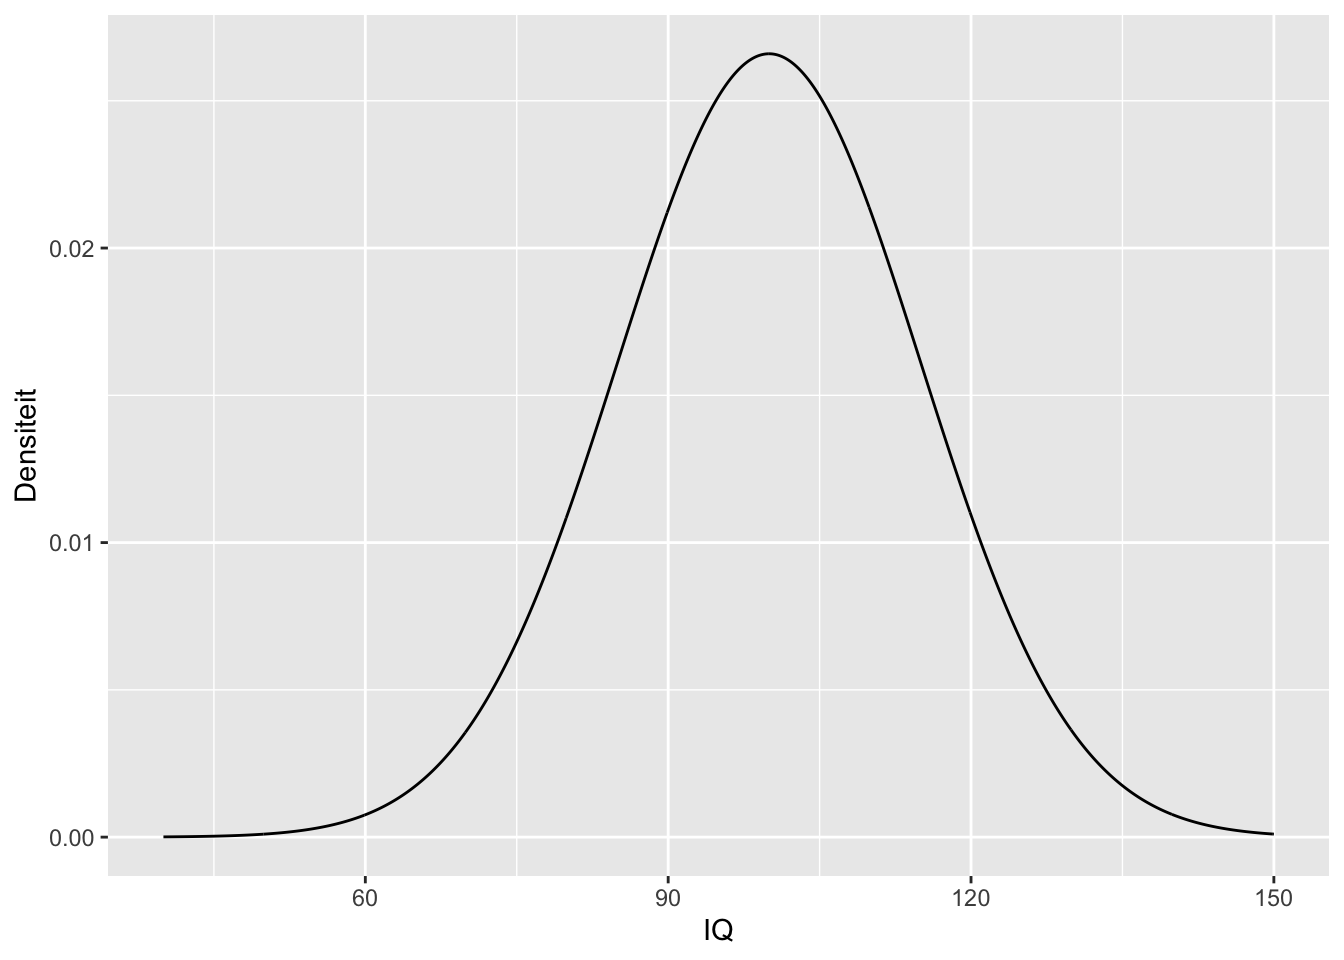
\includegraphics{Statistiek_2020_2021_files/figure-latex/IQ-1} \end{center}

Binnen bepaalde grenzen kunnen continue toevallig veranderlijken alle mogelijke waarden aannemen dus is \(\Omega\) oneindig groot.

\hypertarget{cumulatieve-distributie}{%
\paragraph{Cumulatieve distributie}\label{cumulatieve-distributie}}

Opnieuw is de cumulatieve distributie

\[F(X)=Pr(X\leq x).\]

Omdat X continu is berekenen we deze probabiliteit a.d.h.v. een integraal

\[F(x)=\int \limits_{-\infty}^x f(x) dx\]

Merk op dat \(f(x)=0\) als x niet tot de steekproefruimte behoord.

We kunnen \(F(x)\) berekenen voor een normaal verdeelde toevallig veranderlijke met de functie \texttt{pnorm} die opnieuw argumenten \texttt{mean} en \texttt{sd} heeft.

\begin{Shaded}
\begin{Highlighting}[]
\NormalTok{iq }\OperatorTok{\%\textgreater{}\%}\StringTok{ }\KeywordTok{mutate}\NormalTok{(}\DataTypeTok{Probability =} \KeywordTok{pnorm}\NormalTok{(IQ, }\DataTypeTok{mean =} \DecValTok{100}\NormalTok{, }\DataTypeTok{sd =} \DecValTok{15}\NormalTok{)) }\OperatorTok{\%\textgreater{}\%}\StringTok{ }
\StringTok{    }\KeywordTok{ggplot}\NormalTok{(}\KeywordTok{aes}\NormalTok{(}\DataTypeTok{x =}\NormalTok{ IQ, }\DataTypeTok{y =}\NormalTok{ Probability)) }\OperatorTok{+}\StringTok{ }\KeywordTok{geom\_line}\NormalTok{()}
\end{Highlighting}
\end{Shaded}

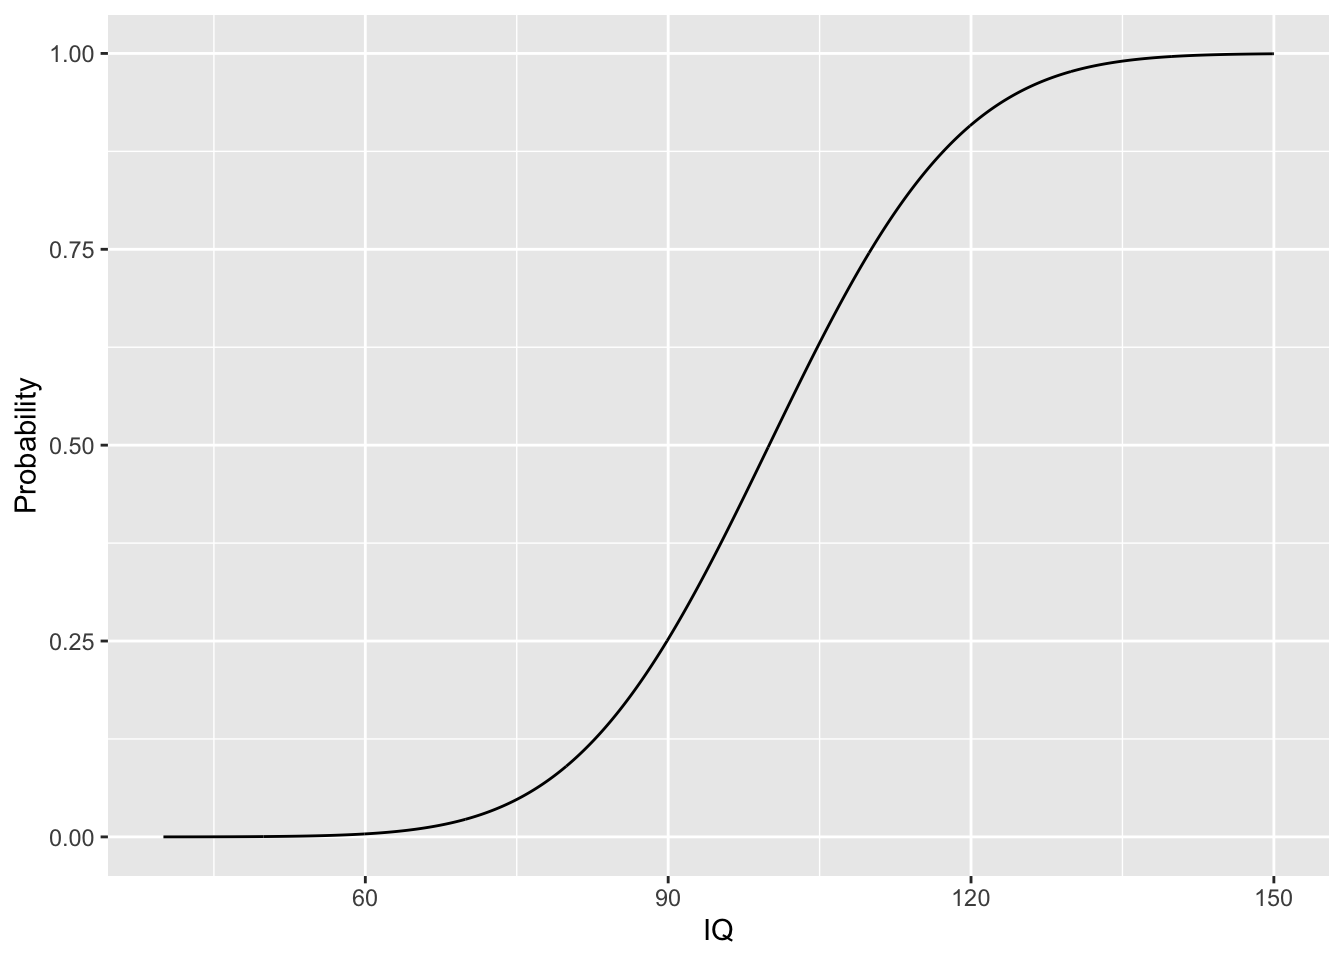
\includegraphics{Statistiek_2020_2021_files/figure-latex/unnamed-chunk-34-1.pdf}

De probabiliteit dat het IQ van een random subject lager is dan 80 wordt in R berekend door

\begin{Shaded}
\begin{Highlighting}[]
\KeywordTok{pnorm}\NormalTok{(}\DecValTok{80}\NormalTok{, }\DataTypeTok{mean =} \DecValTok{100}\NormalTok{, }\DataTypeTok{sd =} \DecValTok{15}\NormalTok{)}
\end{Highlighting}
\end{Shaded}

\begin{verbatim}
## [1] 0.09121122
\end{verbatim}

\begin{center}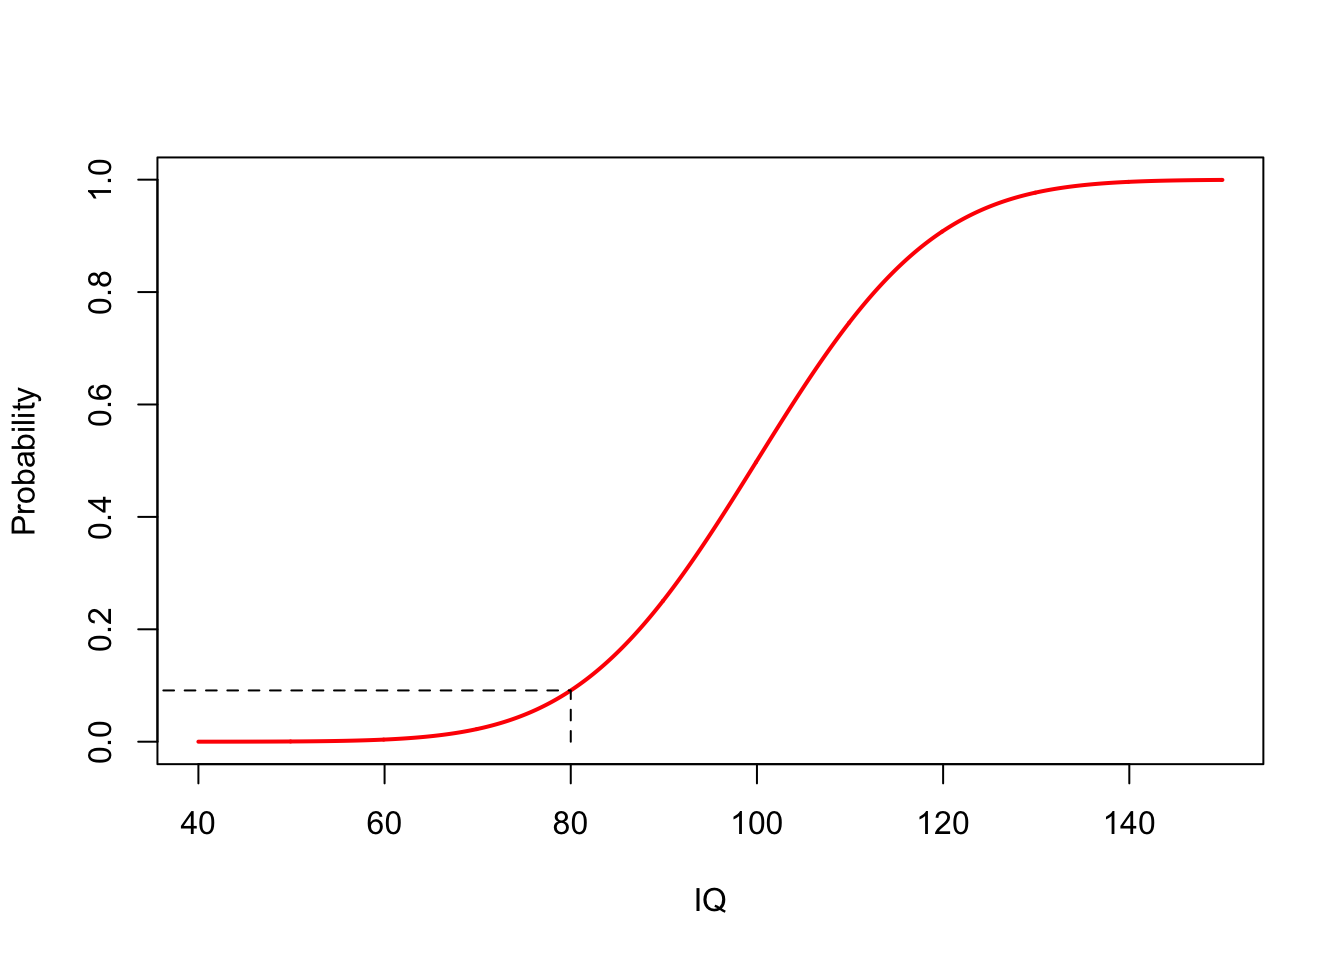
\includegraphics{Statistiek_2020_2021_files/figure-latex/unnamed-chunk-36-1} \end{center}

\begin{center}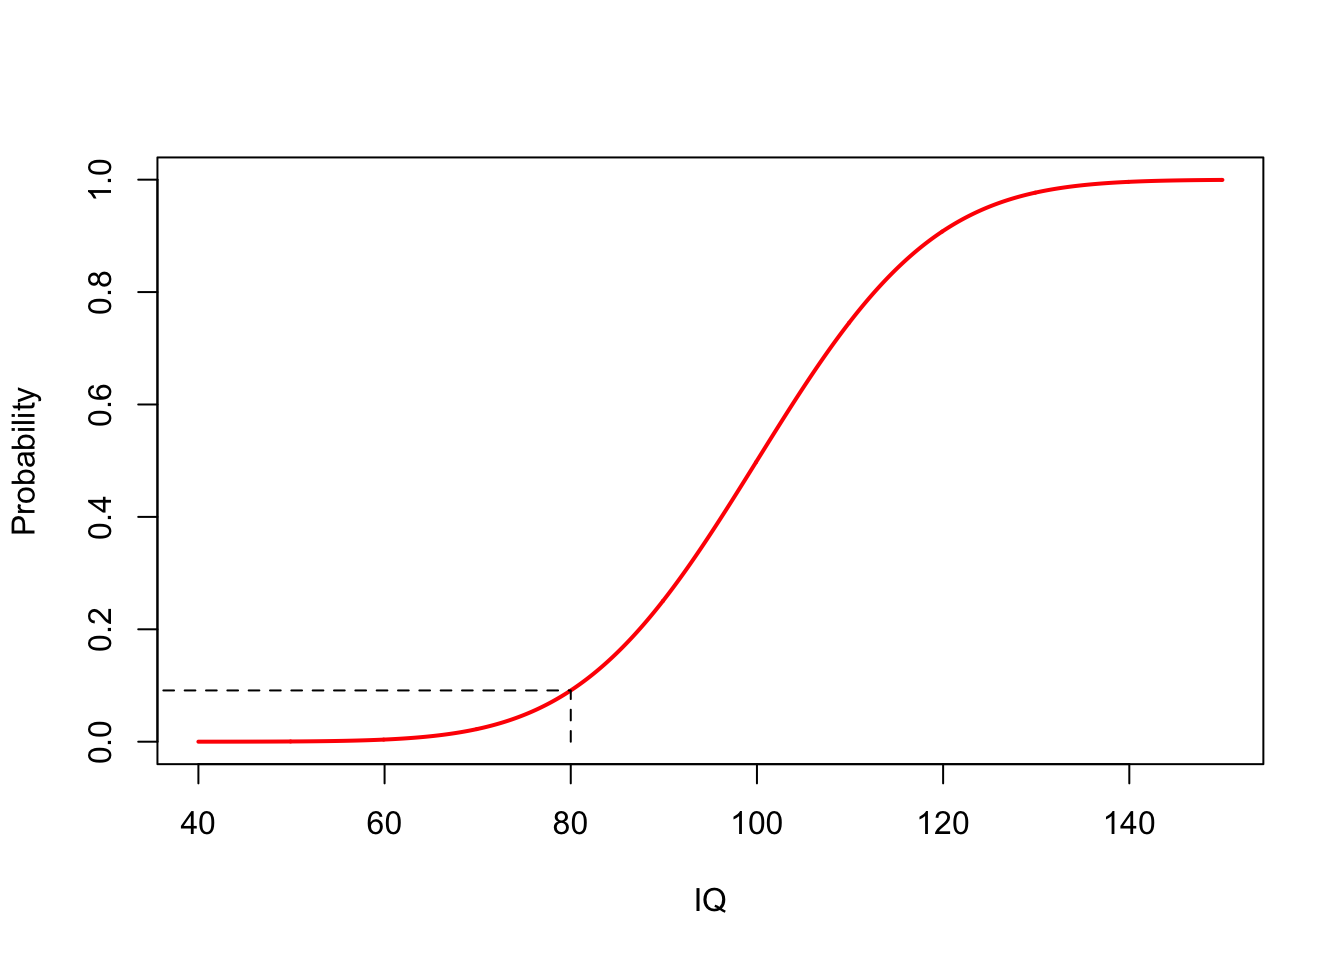
\includegraphics{Statistiek_2020_2021_files/figure-latex/unnamed-chunk-37-1} \end{center}

Voor de grootst mogelijke waarde voor \(X\) integreren we over de volledige steekproefruimte \(\Omega\) dus

\[\int \limits_{x \in \Omega} f(x) dx=1.\]

De oppervlakte onder de dichtheidsfunctie is dus steeds 1!

\hypertarget{gemiddelde-en-variantie}{%
\paragraph{Gemiddelde en variantie}\label{gemiddelde-en-variantie}}

Het gemiddelde of de verwachte waarde is

\[\int \limits_{x \in \Omega} x f(x) dx.\]

Voor de normale distributie

\[\int \limits_{-\infty}^{+\infty} x f(x) dx = \mu.\]

De parameter \(\mu\) is dus het gemiddelde van een Normaal verdeelde veranderlijke X de populatie.

De variance \(E[(X-E[X])^2]\)

\[\int \limits_{x \in \Omega} (x-E[X])^2 f(x) dx\]

Voor de normale distributie bekomen we

\[\int \limits_{-\infty}^{+\infty} (x-\mu)^2 f(x) dx = \sigma^2\]

De parameter \(\sigma^2\) is dus de variantie van een Normaal verdeelde veranderlijke X in de populatie.

Het is vaak moeilijk om de variantie te interpreteren gezien ze niet in de zelfde eenheden staat als het gemiddelde. Daarom werken we vaak met de standaardafwijking (SD):

\[SD=\sqrt{E[(X-E[X])^2]}\]

De standaardafwijking voor de normale distributie, \(\sigma\) heeft de interessante interpretatie dat ongeveer 68\% van de populatie een waarde heeft voor de karakteristiek X binnen het interval van 1 standaardafwijking(\(\sigma\)) rond het gemiddelde:

\[P(\mu-\sigma < X < \mu + \sigma) \approx 0.68\]

\begin{center}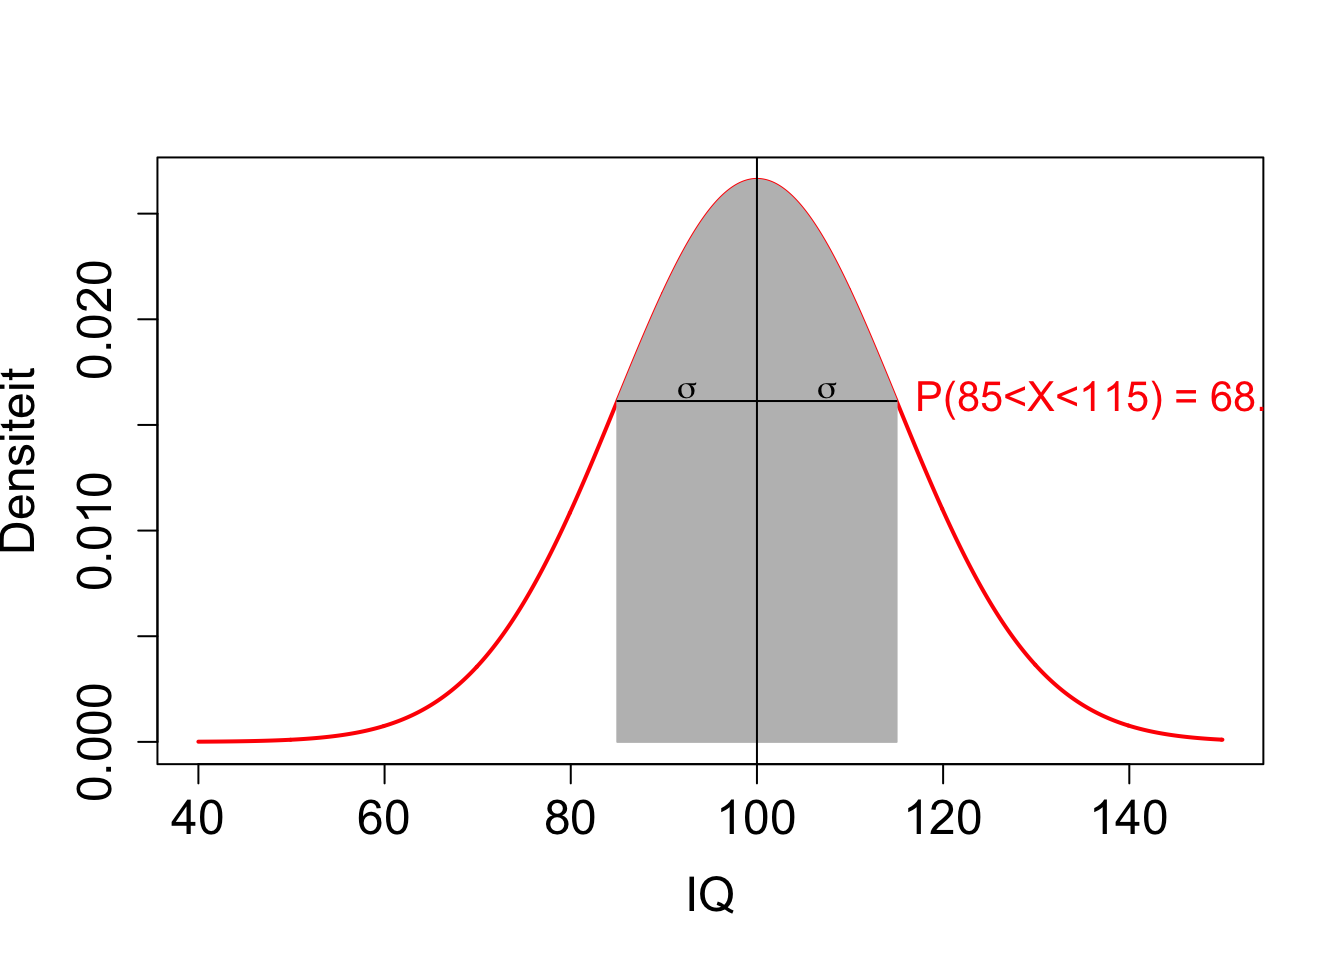
\includegraphics{Statistiek_2020_2021_files/figure-latex/unnamed-chunk-38-1} \end{center}

Voor Normaal verdeelde toevallig veranderlijken heeft ongeveer 95\% van de subjecten in de populatie een waarde die binnen twee standaardafwijkingen (\(2 \sigma\)) ligt van het gemiddelde.

\[P[\mu - 2 \sigma < X < \mu + 2 \sigma]\approx 0.95\]

\begin{center}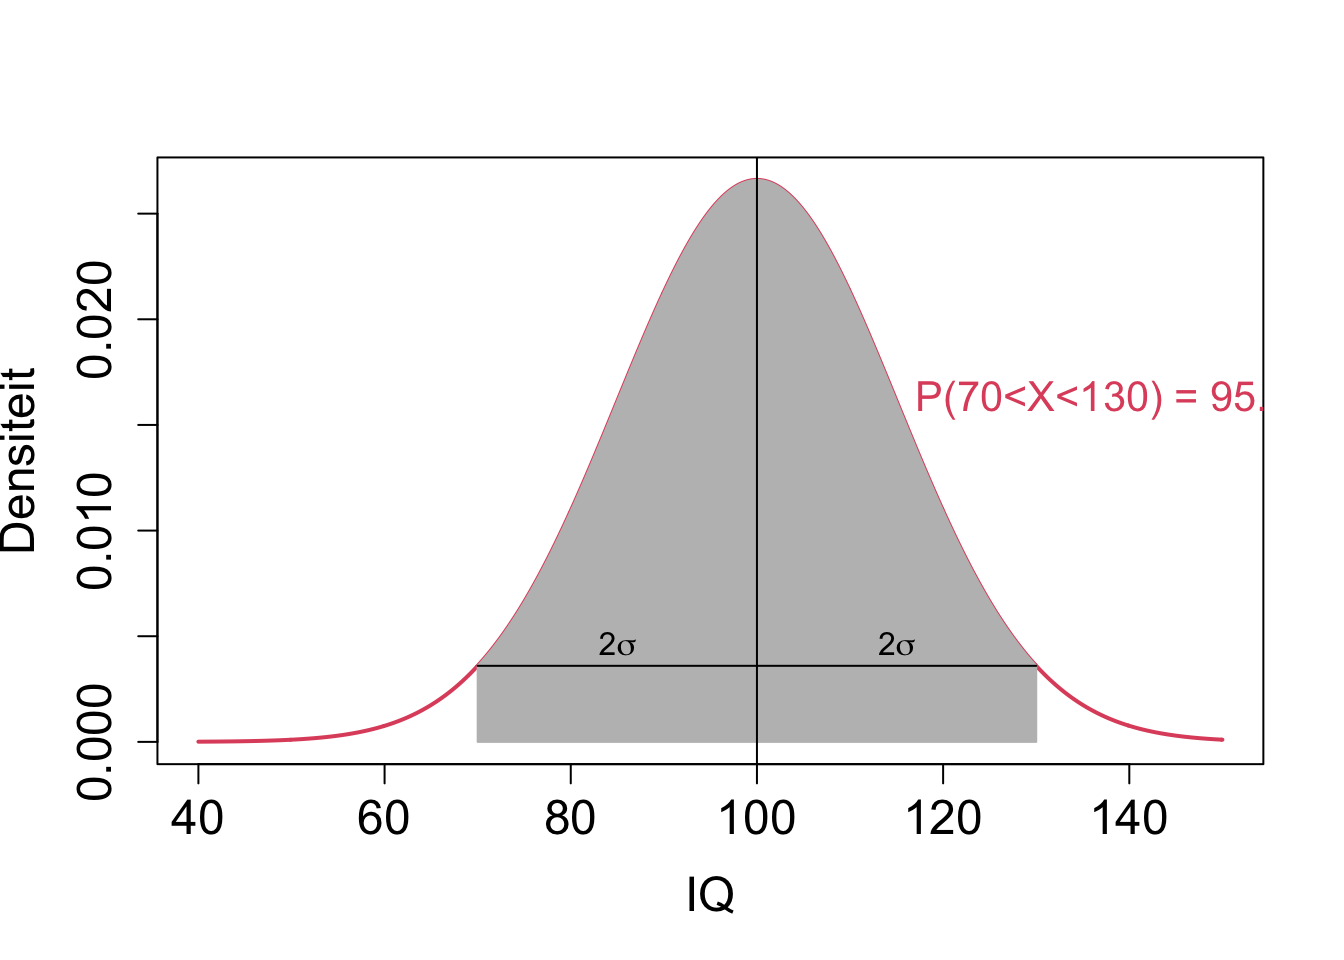
\includegraphics{Statistiek_2020_2021_files/figure-latex/unnamed-chunk-39-1} \end{center}

Deze intervallen worden ook wel een referentie interval genoemd.

\hypertarget{standardisatie}\) en \(z_{97.5\%}\) die respectievelijk corresponderen met \(F(z_{2.5\%})=0.025\) en \(F(z_{97.5\%})=0.975\).

\begin{Shaded}
\begin{Highlighting}[]
\KeywordTok{qnorm}\NormalTok{(}\FloatTok{0.025}\NormalTok{)}
\end{Highlighting}
\end{Shaded}

\begin{verbatim}
## [1] -1.959964
\end{verbatim}

\begin{Shaded}
\begin{Highlighting}[]
\KeywordTok{qnorm}\NormalTok{(}\FloatTok{0.975}\NormalTok{)}
\end{Highlighting}
\end{Shaded}

\begin{verbatim}
## [1] 1.959964
\end{verbatim}

Voor een standaard Normaal verdeelde toevallig veranderlijke valt inderdaad ongeveer \(0.975 - 0.025=0.95\) van de waarden binnen het interval {[}-2,2{]}, of binnen 2 standaardafwijkingen (\(\sigma=1\)) van het gemiddelde (\(\mu=0\)).

\hypertarget{subsec:normalcalc}{%
\subsection{Achtergrond Normale verdeling}\label{subsec:normalcalc}}

De \emph{Normale curve} of \emph{Normale dichtheidsfunctie} wordt gegeven door:

\begin{equation*}
f(x) = \frac{1}{\sigma \sqrt{2 \pi} } \exp \left ( - \frac{ (x - \mu)^2 }{ 2
\sigma^2} \right ).
\end{equation*}

Ze wordt beschreven door 2 onbekende parameters \(\mu\) en \(\sigma\), waarbij \(\mu\) het gemiddelde van de verdeling van de observaties aangeeft en \(\sigma\)
de standaarddeviatie. Deze curve geeft voor elke waarde \(x\) weer hoe
frequent deze waarde, relatief gezien, voorkomt. De notatie \(\pi\) verwijst
naar het getal \(\pi=3.1459...\) Wanneer het gemiddelde 0 is en de variantie
1, spreekt men van de \emph{standaardnormale curve} of \emph{standaardnormale dichtheidsfunctie}.

Een lukrake observatie uit een reeks gegevens wiens verdeling de Normale
curve volgt, wordt een \textbf{Normaal verdeelde observatie} genoemd.
Dergelijke observaties komen frequent voor: voor heel wat reeksen gegevens
die symmetrisch verdeeld zijn, vormt de Normale curve met \(\mu\) gelijk aan \(\bar x\) en \(\sigma\) gelijk aan \(s_x\) immers een goede benadering voor het
histogram.

Voor Normaal verdeelde gegevens geeft de oppervlakte onder de Normale curve
tussen 2 willekeurige getallen \(a\) en \(b\) het percentage van de
observaties weer dat tussen deze 2 getallen gelegen is. Op die manier laat de
Normale curve toe om, enkel op basis van kennis van het gemiddelde en de
standaarddeviatie, na te gaan welk percentage van de gegevens bij benadering
tussen 2 willekeurige getallen \(a\) en \(b\) gelegen is.

Om deze berekening uit te voeren, gaan we als volgt te werk. Zij \(X\) een
lukrake meting uit een reeks Normaal verdeelde gegevens met gemiddelde \(\mu\)
en standaarddeviatie \(\sigma\). Dan noteren we met \(P(X\leq b)\) de
oppervlakte onder de Normale curve die links van \(b\) gelegen is, en met \(P(a\leq X\leq b)\) de oppervlakte onder de Normale curve tussen \(a\) en \(b\).
Hierbij is\footnote{Hierbij maken we gebruik van het feit dat voor een Normaal verdeelde observatie \(X\), \(P(X=a)=0\) voor elk reëel getal \(a\), zodat \(P(X\leq a)=P(X<a)\).}

\begin{equation*}
P(a\leq X\leq b)=P(X\leq b)-P(X\leq a)
\end{equation*}

Om \(P(a\leq X\leq b)\) te berekenen, hebben we dus enkel een strategie nodig
om voor een willekeurig getal \(x\), het getal \(F(x) = P(X \leq x)\) uit te
rekenen. Dit staat uitgezet in functie van \(x\) in Figuur \ref{fig:continu}
(rechtsboven) voor \(\mu=80\) en \(\sigma=12\) en wordt een \emph{distributiefunctie} genoemd.

\begin{definition}[distributiefunctie]
\begin{definition}

\protect\hypertarget{def:unnamed-chunk-41}{}{\label{def:unnamed-chunk-41} \iffalse (distributiefunctie) \fi{} }

\end{definition}
\end{definition}

De functie die voor elk getal \(x\) uitdrukt wat de kans is dat een lukrake
meting \(X\) met gekende verdeling (bvb. een Normale verdeling) kleiner of
gelijk is aan \(x\), wordt de \textbf{distributiefunctie} van die verdeling
genoemd.

\textbf{Einde definitie}

Omdat de Normale dichtheidsfunctie zeer complex is, blijkt dat het getal \(F(x)\) niet expliciet uit te rekenen is. Om die reden heeft men de getallen \(F(x)\)
voor de standaardnormale verdelingsfunctie getabuleerd. Voor
deze standaardnormale curve duidt men voor een willekeurige waarde \(z\), het
getal \(F(z)\) met \(\Phi(z)\) aan. Omwille van de symmetrie rond 0 van de
standaardnormale curve kan de waarde van \(\Phi(-z)\) dan uit de waarde van \(\Phi(z)\) worden afgeleid als

\begin{equation*}
\Phi(-z)= 1- \Phi(z)
\end{equation*}

Deze uitdrukking geeft aan dat voor een reeks standaardnormaal verdeelde
metingen, het percentage dat kleiner is dan \(-z\) gelijk is aan
het percentage dat groter is dan \(z\).

Om nu \(P(a\leq X\leq b)\) te berekenen op basis van de tabellen voor de
standaardnormale verdeling gaan we als volgt te werk. Vooreerst kan men
aantonen dat het resultaat van een lineaire transformatie \(aX+b\) op een
Normaal verdeelde meting \(X\) met gemiddelde \(\mu\) en standaarddeviatie \(\sigma\) terug een Normaal verdeelde meting toevalsveranderlijke is, maar nu
met gemiddelde \(a\mu+b\) en standaarddeviatie \(|a|\sigma\). Op die manier kan
men elke Normaal verdeelde meting met gemiddelde \(\mu\) en standaarddeviatie \(\sigma\) omzetten naar een standaardnormale meting door ze als volgt te
\emph{standaardiseren}:

\begin{equation*}
Z = \frac{X- \mu}{\sigma}
\end{equation*}

Verifieer dat \(Z\) inderdaad gemiddelde 0 en standaarddeviatie 1 heeft!

Aangezien voor een willekeurig getal \(x\)

\begin{equation*}
X\leq x \Leftrightarrow \frac{X-\mu}{\sigma} \leq \frac{x-\mu}{\sigma}
\end{equation*}

vinden we nu dat

\begin{eqnarray*}
P(a \leq X \leq b) & = & P\left(\frac{a-\mu}{\sigma} \leq Z \leq \frac{b-\mu%
}{\sigma} \right) \\
& = & \Phi \left (\frac{b-\mu}{\sigma} \right ) - \Phi \left (\frac{a-\mu}{%
\sigma} \right )
\end{eqnarray*}

De getallen \(\Phi \left (\frac{b-\mu}{\sigma} \right )\) en \(\Phi \left (\frac{a-\mu}{\sigma} \right )\) kunnen hierbij rechtstreeks uit tabellen of R software worden gehaald. In het vervolg zullen we
algemeen de notatie \(Z\) gebruiken om een standaardnormaal verdeelde meting
aan te duiden.

\begin{exercise}
\begin{exercise}

\protect\hypertarget{exr:unnamed-chunk-42}{}{\label{exr:unnamed-chunk-42} }

\end{exercise}
\end{exercise}

Een labo bepaalt in een visstaal Hg via een methode op basis van AAS. In
werkelijkheid bevat het staal (gemiddeld) 1.90 ppm. De meetmethode is echter
niet perfect, zoals aangegeven door een standaarddeviatie van 0.10 ppm. Wat
is de kans dat de laborant die het staal onderzoekt, een meetresultaat van
2.10 ppm of meer vaststelt?

Om op deze vraag te antwoorden, noteren we met \(X\) het meetresultaat van de
laborant en berekenen we

\begin{eqnarray*}
P(X\geq 2)&=&P\left(\frac{X-\mu}{\sigma}\geq \frac{2.1-1.9}{0.1}\right) \\
&=&P(Z\geq 2) = 2.28\%
\end{eqnarray*}

We besluiten dat er 2.28\% kans is dat de laborant een meetresultaat van
minstens 2.10 ppm zal vaststellen. In R kan dit resultaat als volgt bekomen worden:

\begin{Shaded}
\begin{Highlighting}[]
\DecValTok{1} \OperatorTok{{-}}\StringTok{ }\KeywordTok{pnorm}\NormalTok{(}\FloatTok{2.1}\NormalTok{, }\DataTypeTok{mean =} \FloatTok{1.9}\NormalTok{, }\DataTypeTok{sd =} \FloatTok{0.1}\NormalTok{)}
\end{Highlighting}
\end{Shaded}

\begin{verbatim}
## [1] 0.02275013
\end{verbatim}

waarbij de functie pnorm de distributiefunctie van de Normale verdeling voorstelt.

\textbf{Einde oefening}

Met \(z_{\alpha}\) duiden\footnote{Let wel op want in verschillende boeken krijgt het symbool \(z_{\alpha}\) verschillende definities!} we die waarde aan waar \(\alpha100\%\) van de
oppervlakte onder de standaardnormale curve rechts van zit; m.a.w. waarvoor
geldt dat \(P(Z \geq z_{\alpha}) = \alpha\). Als \(Z\) een standaardnormaal
verdeelde meting is, dan stelt \(z_{\alpha}\) bijgevolg het \((1-\alpha)100\%\)
percentiel van die verdeling voor. Voor \(z_{\alpha/2}\) geldt dat \(P(-z_{\alpha/2}\leq Z \leq z_{\alpha/2}) = 1-\alpha\). Bijvoorbeeld, \(P( - z_{0.025}\leq Z \leq z_{0.025}) = 95\%\). Voor een reeks standaardnormaal
verdeelde metingen bevat het interval \([-z_{\alpha/2},z_{\alpha/2}]\) dus \((1-\alpha)100\%\) van de observaties.

Stel dat \(X\) een Normaal verdeelde meting is met gemiddelde \(\mu\) en
standaarddeviatie \(\sigma\). Dan geldt dat

\begin{equation*}
P\left( - z_{\alpha/2}\leq \frac{X - \mu}{\sigma} \leq z_{\alpha/2}\right) =
1-\alpha .
\end{equation*}

Hieruit volgt dat

\begin{equation*}
P( \mu - z_{\alpha/2} \sigma \leq X \leq \mu + z_{\alpha/2} \sigma ) =
1-\alpha .
\end{equation*}

Voor een reeks Normaal verdeelde metingen met gemiddelde \(\mu\) en
standaarddeviatie \(\sigma\) bevat het interval \([\mu-z_{\alpha/2}\sigma,\mu+z_{\alpha/2}\sigma]\) dus \((1-\alpha)100\%\) van de observaties. In de
praktijk worden de parameters \(\mu\) en \(\sigma\) hierbij vervangen door \(\bar x\) en \(s_x\).

Het resulterende interval \([\bar x-z_{\alpha/2}s_x,\bar x+z_{\alpha/2}s_x]\)
wordt vaak gebruikt\footnote{Dit interval bevat niet exact \((1-\alpha)100\%\) van de observaties, maar slechts bij benadering, omdat het geen rekening houdt met het feit dat \(\bar x\) en \(\sigma_x\) impreciese schattingen zijn voor \(\mu\) en \(\sigma\) op basis van een eindige steekproef. Meer accurate referentie-intervallen die deze imprecisie in rekening brengen, ook predictie-intervallen genoemd}, o.a. in de klinische chemie, om \emph{referentie-intervallen} te berekenen voor een test ter opsporing van een
bepaalde pathologie. Eenmaal zo'n referentie-interval, ook wel \emph{normaal interval} genoemd, werd bepaald, wordt het testresultaat van een
patiënt met de vermoede pathologie vergeleken met het interval. Een
resultaat buiten het interval is dan indicatief voor de aanwezigheid van de
pathologie.

Bij het bepalen van referentie-intervallen is het noodzakelijk om de methode
eerst te testen bij mensen zonder de pathologie in kwestie. Voor dit doel
worden `normale en gezonde vrijwilligers' aangezocht. Vaak worden hiertoe
collega's genomen uit het laboratorium dat de test heeft ontwikkeld, hoewel
dit allesbehalve ideaal is. Immers, mensen die in een zelfde laboratorium
werken, zijn blootgesteld aan dezelfde werkomgeving, die op zijn beurt een
invloed kan hebben op hun bloedsamenstelling. Bijgevolg is de
bloedsamenstelling van de studiepersonen mogelijks niet representatief voor
een normale, gezonde populatie, hetgeen kan leiden tot vertekende
referentie-intervallen. In deze cursus zullen we een referentie-interval
meer algemeen als volgt definiëren.

\begin{definition}[referentie-interval]
\begin{definition}

\protect\hypertarget{def:unnamed-chunk-44}{}{\label{def:unnamed-chunk-44} \iffalse (referentie-interval) \fi{} }

\end{definition}
\end{definition}

Een \textbf{\((1-\alpha)100\%\) referentie-interval}
voor een veranderlijke \(X\) (bvb. albumine-concentratie
in het bloed) in een gegeven studiepopulatie (bvb. volwassen Belgen onder de
60 jaar) is een interval dat zó gekozen werd dat het met \((1-\alpha)100\%\)
kans de observatie voor een lukraak individu uit die populatie bevat. Voor
een Normaal verdeelde veranderlijke \(X\) met gemiddelde \(\mu\) en
standaarddeviatie \(\sigma\) kan dit berekend worden als

\begin{equation*}
[\mu-z_{\alpha/2}\sigma,\mu+z_{\alpha/2}\sigma]
\end{equation*}

en geschat worden op basis van een lukrake steekproef als

\begin{equation*}
[\bar x-z_{\alpha/2}s_x,\bar x+z_{\alpha/2}s_x]
\end{equation*}

\textbf{Einde definitie}

\hypertarget{steekproef}{%
\section{Steekproef}\label{steekproef}}

In echte studies kennen we de verdeling in de populatie typisch niet!
In de praktijk is het om financiële en logistieke redenen bijna nooit mogelijk om de
volledige populatie te bestuderen. Populatieparameters (v.b. gemiddeld IQ, variantie van IQ) kunnen daarom meestal
niet exact bepaald worden. Enkel een deel van de populatie kan onderzocht
worden, hetgeen men de \emph{steekproef} noemt. Volgens een
gestructureerd design worden daartoe \textbf{lukraak subjecten} uit de doelpopulatie
getrokken en geobserveerd. De onbekende parameters worden vervolgens geschat
o.b.v. die steekproef en noemt met schattingen. In de praktijk hoopt men uiteraard dat de schattingen die men bekomt op basis van de steekproef vergelijkbaar zijn met de overeenkomstige populatieparameters die men voor de volledige populatie zou bekomen.

Stel bijvoorbeeld dat we op basis van de NHANES studie de lengte van volgroeide vrouwen en mannen wensen te bestuderen.
Telkens een lukraak individu getrokken wordt uit de populatie zal men een
realisatie van de toevalsveranderlijke \(X\) kunnen observeren. Die realisatie
of geobserveerde waarde duiden we aan met een kleine letter \(x\). Deze stelt
dus een welbepaald getal voor en is niet langer een onbekende veranderlijke
zoals \(X\). Samengevat zijn de nog onbekende waarden voor de
bestudeerde populatiekarakteristiek bij subjecten 1 tot \(n\) in de
steekproef, toevalsveranderlijken die we algemeen met \(X_1,...,X_n\)
zullen noteren. Na het trekken van de steekproef, ziet men de gerealiseerde
uitkomsten \(x_1, x_2, \dots, x_n\), bijvoorbeeld hun gemeten lengte.

De distributie in de populatie is ongekend en moet worden geschat op basis van de steekproef. Als we aannemen dat de gegevens een bepaalde distributie volgen (b.v. de normale verdeling \(N(\mu,\sigma^2)\)) dan moeten we enkel de populatie parameters (\(\mu\) en \(\sigma^2\)) schatten op basis van de steekproef. We noemen dit schattingen (engels: estimates) en noteren ze als volgt: \(\hat \mu\) en \(\hat \sigma^2\).

\emph{Samenvatting}

\begin{itemize}
\item
  Voor we het experiment uitvoeren is de populatie karakteristiek voor de proefpersonen \(1,\ldots,n\) die we uit de populatie zullen trekken ongekend en zijn dat toevallig veranderlijken: \(X_1, \ldots, X_n\)
\item
  Dit is noodzakelijk om te kunnen redeneren over hoe de resultaten van steekproef tot steekproef kunnen wijzigen
\item
  In een steekproef observeren we gerealiseerde uitkomsten \(x_1, x_2, \dots, x_n\): v.b. gender of lengte van subjecten in de steekproef.
\end{itemize}

\hypertarget{nhanes-gender}{%
\section{NHANES: Gender}\label{nhanes-gender}}

\begin{Shaded}
\begin{Highlighting}[]
\KeywordTok{library}\NormalTok{(NHANES)}
\NormalTok{NHANES }\OperatorTok{\%\textgreater{}\%}\StringTok{ }\KeywordTok{ggplot}\NormalTok{(}\KeywordTok{aes}\NormalTok{(}\DataTypeTok{x =}\NormalTok{ Gender)) }\OperatorTok{+}\StringTok{ }\KeywordTok{geom\_bar}\NormalTok{()}
\end{Highlighting}
\end{Shaded}

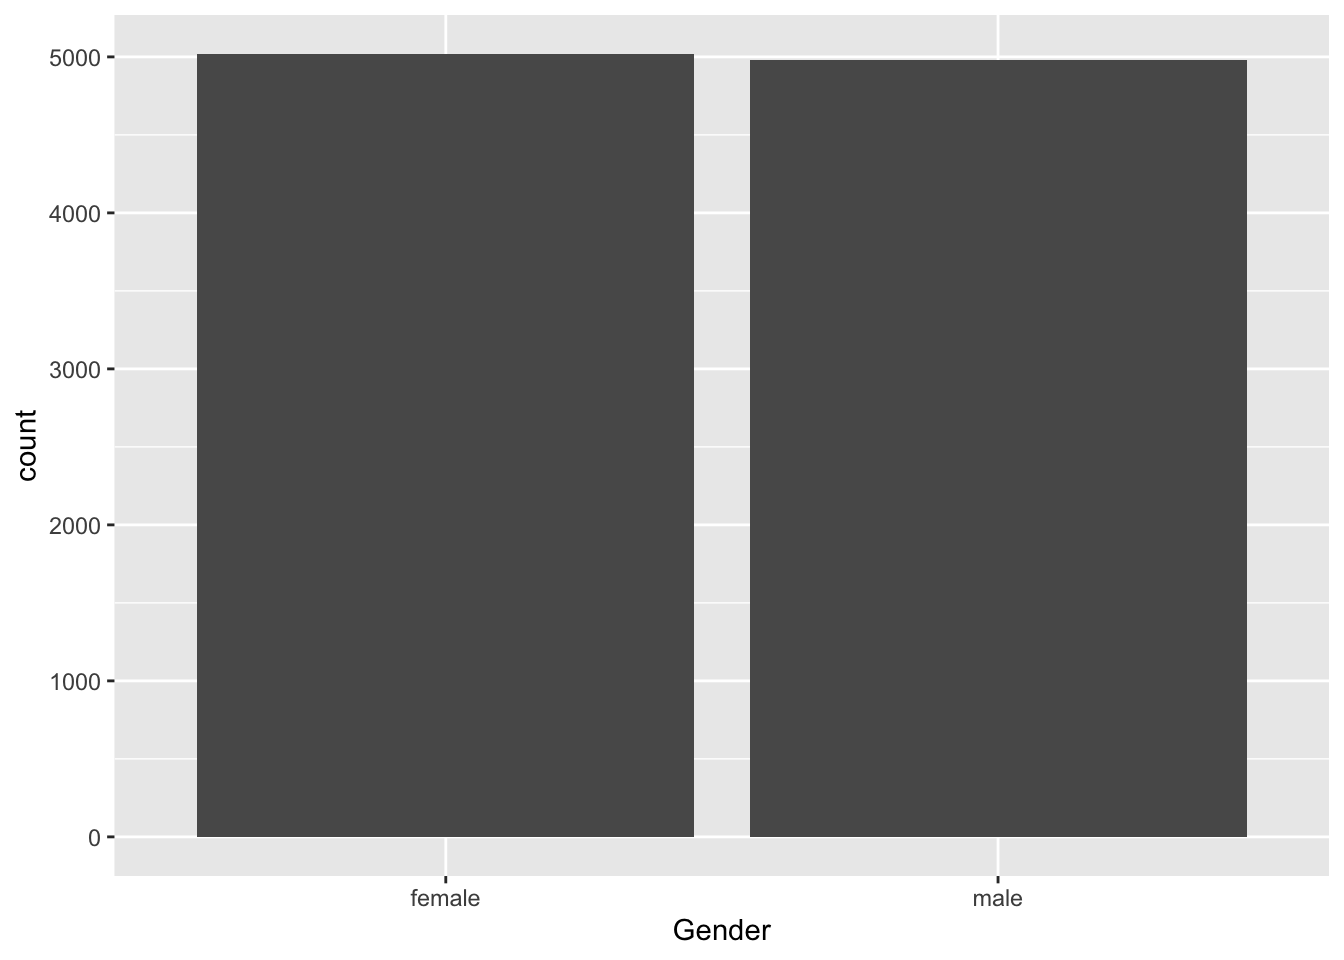
\includegraphics{Statistiek_2020_2021_files/figure-latex/unnamed-chunk-45-1.pdf}

\begin{itemize}
\tightlist
\item
  Gender is een binaire variabele.
\item
  Het volgt een Bernoulli distibutie.
\item
  De Bernoulli distributie heeft een parameter: het gemiddelde \(\pi\).
\item
  We kunnen \(\pi\) schatten op basis van de steekproef door het steekproefgemiddelde te berekenen \(\bar x = \sum\limits_{i=1}^n x_i\)
\item
  Merk op dat het steekproefgemiddelde zelf een toevallig veranderlijke is! Het wijzigt ook van steekproef tot steekproef!
\end{itemize}

\begin{Shaded}
\begin{Highlighting}[]
\NormalTok{NHANES }\OperatorTok{\%\textgreater{}\%}\StringTok{ }\KeywordTok{count}\NormalTok{(Gender) }\OperatorTok{\%\textgreater{}\%}\StringTok{ }\KeywordTok{mutate}\NormalTok{(}\DataTypeTok{probability =}\NormalTok{ n}\OperatorTok{/}\KeywordTok{sum}\NormalTok{(n))}
\end{Highlighting}
\end{Shaded}

\begin{verbatim}
## # A tibble: 2 x 3
##   Gender     n probability
##   <fct>  <int>       <dbl>
## 1 female  5020       0.502
## 2 male    4980       0.498
\end{verbatim}

\hypertarget{nhanes-lengte}{%
\section{NHANES: Lengte}\label{nhanes-lengte}}

\hypertarget{empirische-distributie}{%
\subsection{Empirische distributie}\label{empirische-distributie}}

We kunnen de distributie van de lengte voor volwassen vrouwen schatten aan de hand van het histogram.

\begin{Shaded}
\begin{Highlighting}[]
\NormalTok{NHANES }\OperatorTok{\%\textgreater{}\%}\StringTok{ }\KeywordTok{filter}\NormalTok{(Gender }\OperatorTok{==}\StringTok{ "female"} \OperatorTok{\&}\StringTok{ }\OperatorTok{!}\KeywordTok{is.na}\NormalTok{(Height) }\OperatorTok{\&}\StringTok{ }
\StringTok{    }\NormalTok{Age }\OperatorTok{\textgreater{}}\StringTok{ }\DecValTok{18}\NormalTok{) }\OperatorTok{\%\textgreater{}\%}\StringTok{ }\KeywordTok{ggplot}\NormalTok{(}\KeywordTok{aes}\NormalTok{(}\DataTypeTok{x =}\NormalTok{ Height)) }\OperatorTok{+}\StringTok{ }\KeywordTok{geom\_histogram}\NormalTok{()}
\end{Highlighting}
\end{Shaded}

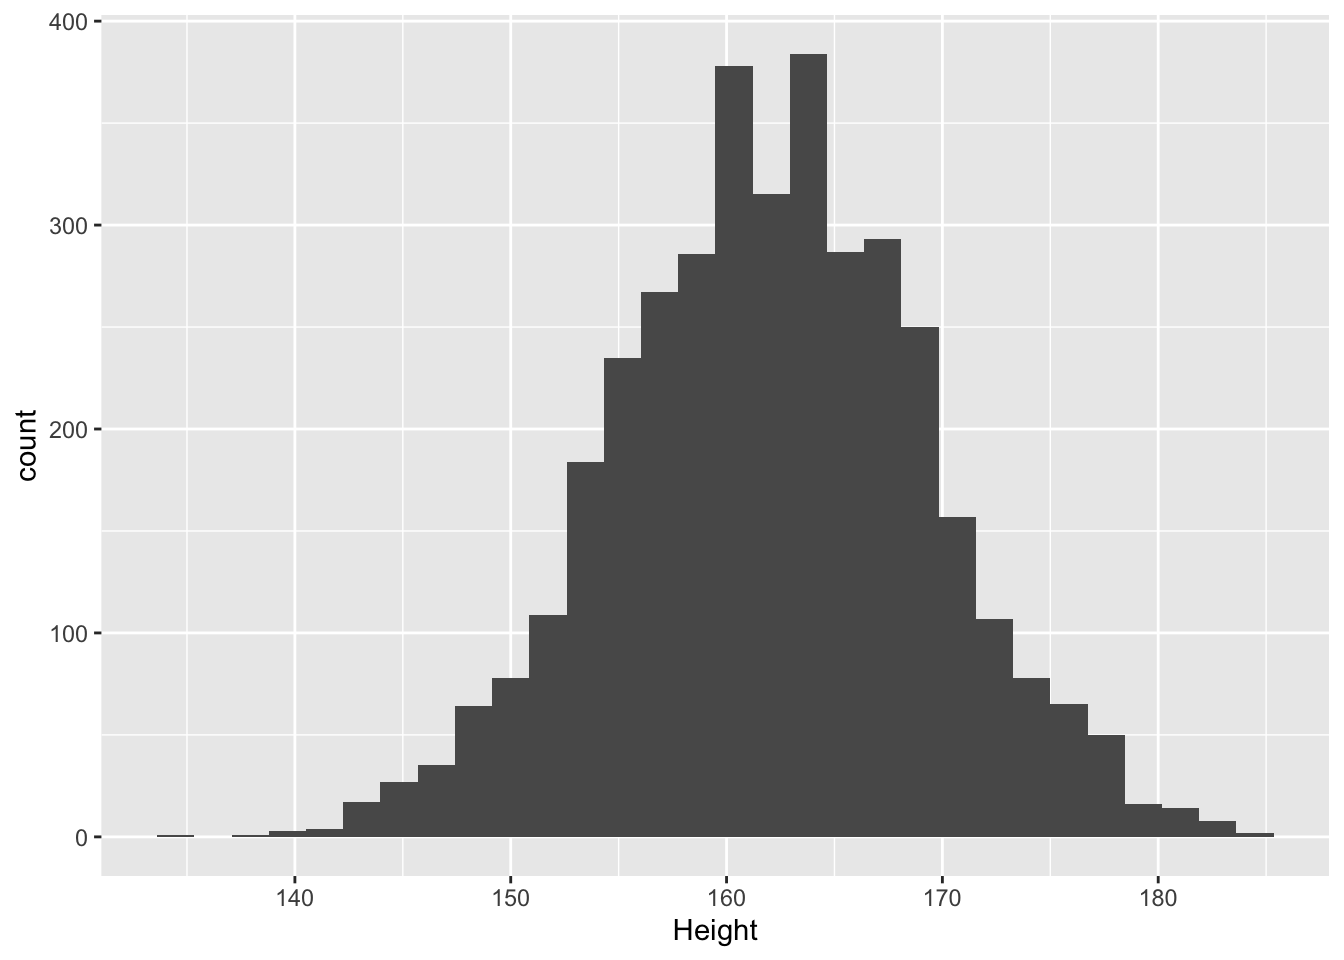
\includegraphics{Statistiek_2020_2021_files/figure-latex/unnamed-chunk-47-1.pdf}

We kunnen de cumulative distributie functie schatten door gebruik te maken van de empirische cumulatieve distributie functie.
- Elke observatie werd één keer geobserveerd in het staal.
- Dus empirische cumulatieve distributie functie van het staal is een discrete distributie met probabiliteit 1/n op elke observatie.
- De empirische cumulatieve distributie functie (ECDF) is gegeven door

\begin{verbatim}
$$ECDF(x) = \sum\limits_{x_i \leq x} \frac{1}{n} = \frac{\# (x_i \leq x)}{n}$$
\end{verbatim}

\begin{Shaded}
\begin{Highlighting}[]
\NormalTok{NHANES }\OperatorTok{\%\textgreater{}\%}\StringTok{ }\KeywordTok{filter}\NormalTok{(Gender }\OperatorTok{==}\StringTok{ "female"} \OperatorTok{\&}\StringTok{ }\OperatorTok{!}\KeywordTok{is.na}\NormalTok{(Height) }\OperatorTok{\&}\StringTok{ }
\StringTok{    }\NormalTok{Age }\OperatorTok{\textgreater{}}\StringTok{ }\DecValTok{18}\NormalTok{) }\OperatorTok{\%\textgreater{}\%}\StringTok{ }\KeywordTok{ggplot}\NormalTok{(}\KeywordTok{aes}\NormalTok{(}\DataTypeTok{x =}\NormalTok{ Height)) }\OperatorTok{+}\StringTok{ }\KeywordTok{stat\_ecdf}\NormalTok{()}
\end{Highlighting}
\end{Shaded}

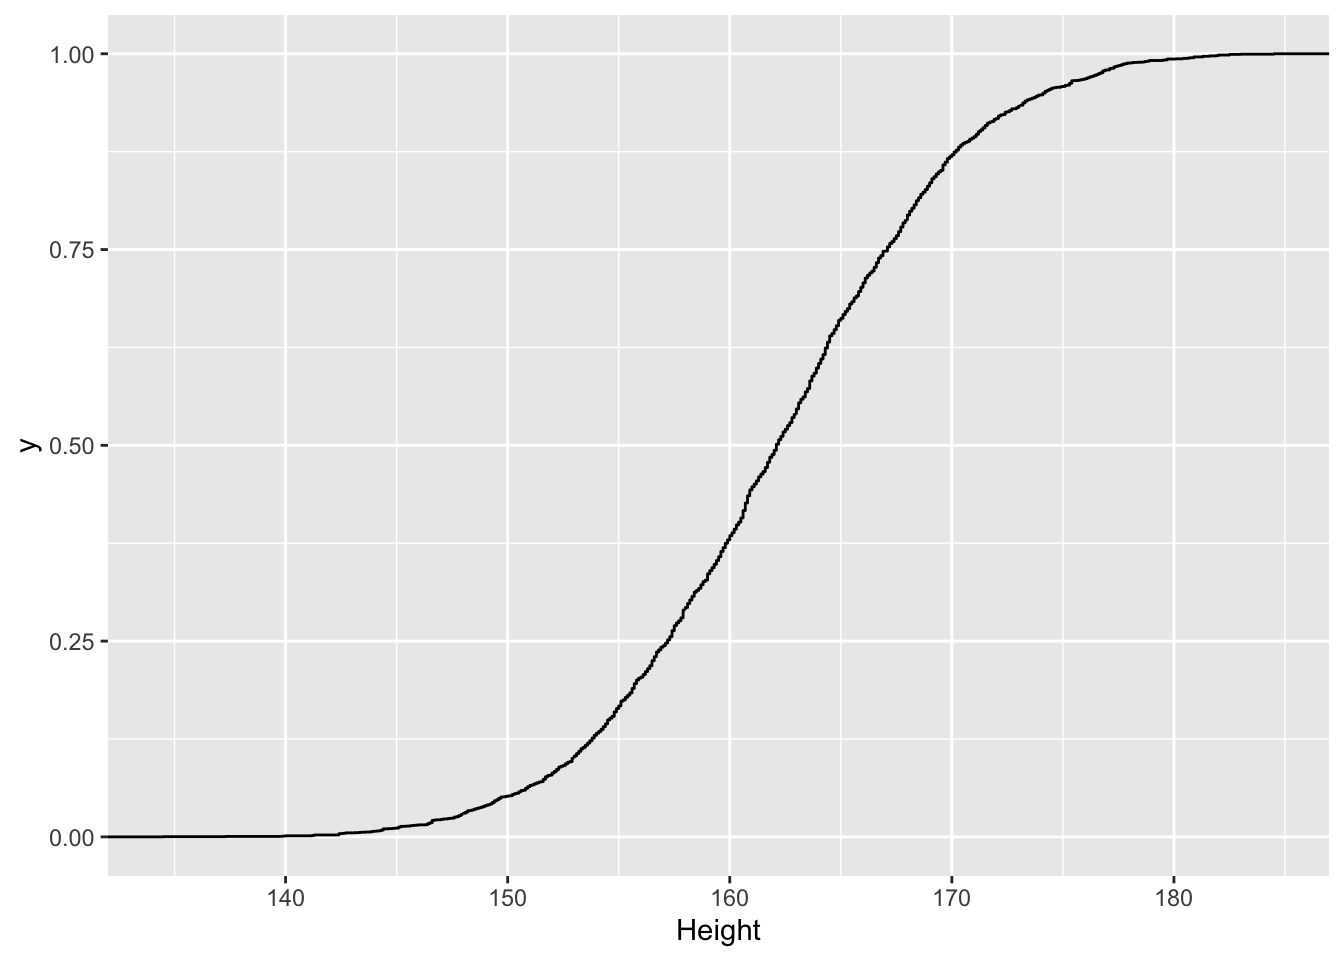
\includegraphics{Statistiek_2020_2021_files/figure-latex/unnamed-chunk-48-1.pdf}

We kunnen de empische cumulatieve distributie functie gebruiken om kansen te berekenen.
Wat is de kans dat een vrouw kleiner is dan 150 cm.

\begin{Shaded}
\begin{Highlighting}[]
\NormalTok{ecdfFem \textless{}{-}}\StringTok{ }\NormalTok{NHANES }\OperatorTok{\%\textgreater{}\%}\StringTok{ }\KeywordTok{filter}\NormalTok{(Gender }\OperatorTok{==}\StringTok{ "female"} \OperatorTok{\&}\StringTok{ }\OperatorTok{!}\KeywordTok{is.na}\NormalTok{(Height) }\OperatorTok{\&}\StringTok{ }
\StringTok{    }\NormalTok{Age }\OperatorTok{\textgreater{}}\StringTok{ }\DecValTok{18}\NormalTok{) }\OperatorTok{\%\textgreater{}\%}\StringTok{ }\KeywordTok{pull}\NormalTok{(}\StringTok{"Height"}\NormalTok{) }\OperatorTok{\%\textgreater{}\%}\StringTok{ }\NormalTok{ecdf}
\KeywordTok{ecdfFem}\NormalTok{(}\DecValTok{150}\NormalTok{)}
\end{Highlighting}
\end{Shaded}

\begin{verbatim}
## [1] 0.05222073
\end{verbatim}

We illustreren dit ook voor een steekproef van grootte 10

\begin{Shaded}
\begin{Highlighting}[]
\KeywordTok{set.seed}\NormalTok{(}\DecValTok{502}\NormalTok{)}
\NormalTok{fem10 \textless{}{-}}\StringTok{ }\NormalTok{NHANES }\OperatorTok{\%\textgreater{}\%}\StringTok{ }\KeywordTok{filter}\NormalTok{(Gender }\OperatorTok{==}\StringTok{ "female"} \OperatorTok{\&}\StringTok{ }\OperatorTok{!}\KeywordTok{is.na}\NormalTok{(Height) }\OperatorTok{\&}\StringTok{ }
\StringTok{    }\NormalTok{Age }\OperatorTok{\textgreater{}}\StringTok{ }\DecValTok{18}\NormalTok{) }\OperatorTok{\%\textgreater{}\%}\StringTok{ }\KeywordTok{sample\_n}\NormalTok{(}\DataTypeTok{size =} \DecValTok{10}\NormalTok{)}

\NormalTok{fem10 }\OperatorTok{\%\textgreater{}\%}\StringTok{ }\KeywordTok{ggplot}\NormalTok{(}\KeywordTok{aes}\NormalTok{(}\DataTypeTok{x =}\NormalTok{ DirectChol)) }\OperatorTok{+}\StringTok{ }\KeywordTok{stat\_ecdf}\NormalTok{()}
\end{Highlighting}
\end{Shaded}

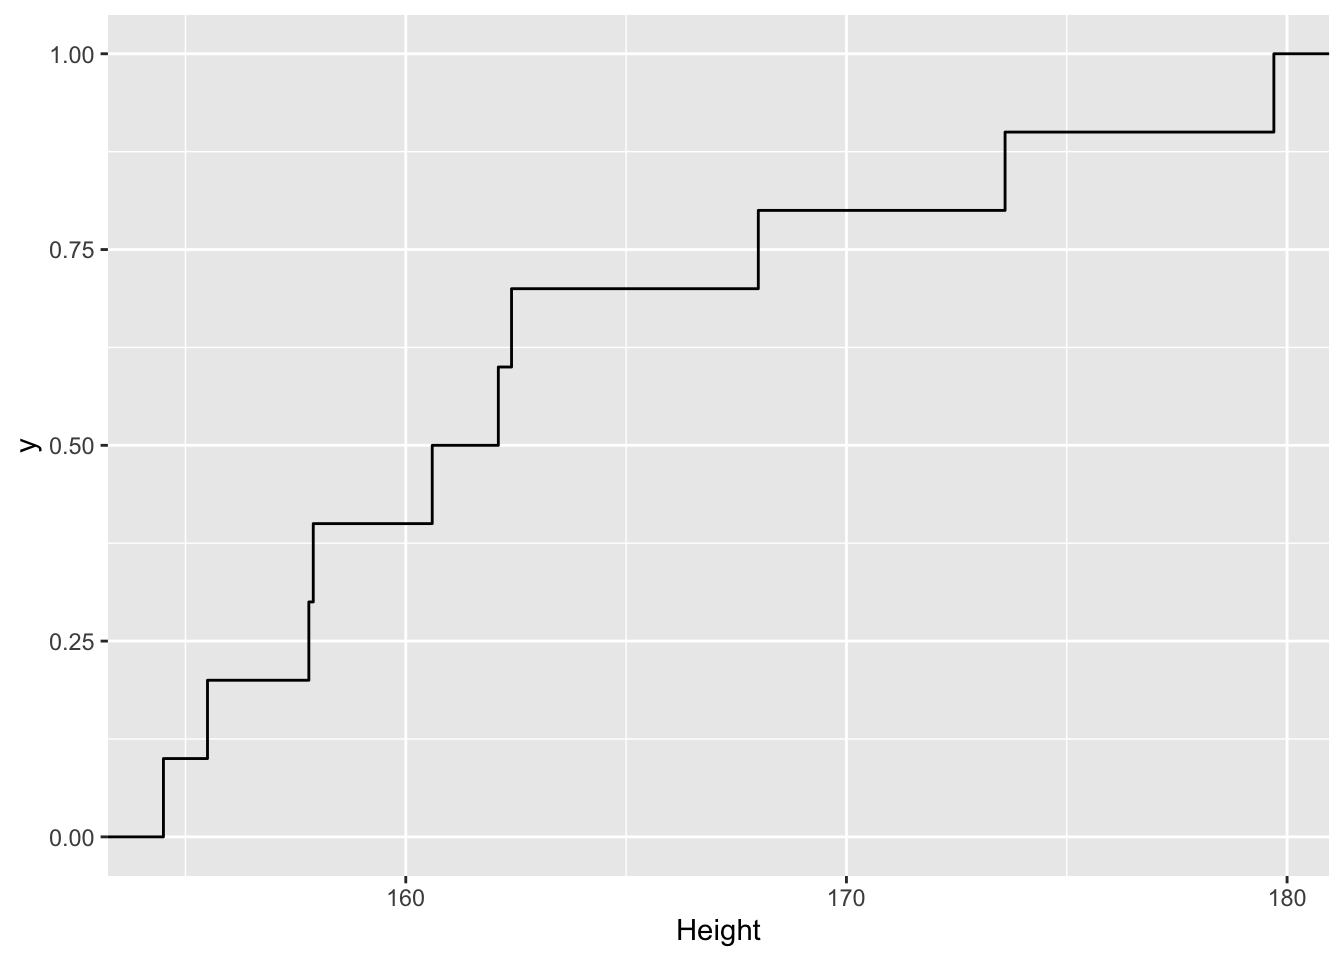
\includegraphics{Statistiek_2020_2021_files/figure-latex/unnamed-chunk-50-1.pdf}

\begin{Shaded}
\begin{Highlighting}[]
\NormalTok{ecdfFem10 \textless{}{-}}\StringTok{ }\NormalTok{fem10 }\OperatorTok{\%\textgreater{}\%}\StringTok{ }\KeywordTok{pull}\NormalTok{(Height) }\OperatorTok{\%\textgreater{}\%}\StringTok{ }\NormalTok{ecdf}
\KeywordTok{ecdfFem10}\NormalTok{(}\DecValTok{150}\NormalTok{)}
\end{Highlighting}
\end{Shaded}

\begin{verbatim}
## [1] 0
\end{verbatim}

Merk op dat die kans niet goed wordt geschat o.b.v. de kleine steekproef. Er zijn immers te weinig observaties om de kansen goed te kunnen schatten.

Merk ook op dat we die kans ook hadden kunnen schatten door te berekenen hoeveel lengtemetingen er lager zijn dan 150.

\begin{Shaded}
\begin{Highlighting}[]
\NormalTok{NHANES }\OperatorTok{\%\textgreater{}\%}\StringTok{ }\KeywordTok{filter}\NormalTok{(Gender }\OperatorTok{==}\StringTok{ "female"} \OperatorTok{\&}\StringTok{ }\OperatorTok{!}\KeywordTok{is.na}\NormalTok{(Height) }\OperatorTok{\&}\StringTok{ }
\StringTok{    }\NormalTok{Age }\OperatorTok{\textgreater{}}\StringTok{ }\DecValTok{18}\NormalTok{) }\OperatorTok{\%\textgreater{}\%}\StringTok{ }\KeywordTok{count}\NormalTok{(Height }\OperatorTok{\textless{}=}\StringTok{ }\DecValTok{150}\NormalTok{) }\OperatorTok{\%\textgreater{}\%}\StringTok{ }\KeywordTok{mutate}\NormalTok{(}\DataTypeTok{prob =}\NormalTok{ n}\OperatorTok{/}\KeywordTok{sum}\NormalTok{(n))}
\end{Highlighting}
\end{Shaded}

\begin{verbatim}
## # A tibble: 2 x 3
##   `Height <= 150`     n   prob
##   <lgl>           <int>  <dbl>
## 1 FALSE            3521 0.948 
## 2 TRUE              194 0.0522
\end{verbatim}

\begin{Shaded}
\begin{Highlighting}[]
\KeywordTok{ecdfFem}\NormalTok{(}\DecValTok{150}\NormalTok{)}
\end{Highlighting}
\end{Shaded}

\begin{verbatim}
## [1] 0.05222073
\end{verbatim}

\begin{Shaded}
\begin{Highlighting}[]
\NormalTok{fem10 }\OperatorTok{\%\textgreater{}\%}\StringTok{ }\KeywordTok{count}\NormalTok{(Height }\OperatorTok{\textless{}=}\StringTok{ }\DecValTok{150}\NormalTok{) }\OperatorTok{\%\textgreater{}\%}\StringTok{ }\KeywordTok{mutate}\NormalTok{(}\DataTypeTok{prob =}\NormalTok{ n}\OperatorTok{/}\KeywordTok{sum}\NormalTok{(n))}
\end{Highlighting}
\end{Shaded}

\begin{verbatim}
## # A tibble: 1 x 3
##   `Height <= 150`     n  prob
##   <lgl>           <int> <dbl>
## 1 FALSE              10     1
\end{verbatim}

\begin{Shaded}
\begin{Highlighting}[]
\KeywordTok{ecdfFem10}\NormalTok{(}\DecValTok{150}\NormalTok{)}
\end{Highlighting}
\end{Shaded}

\begin{verbatim}
## [1] 0
\end{verbatim}

\hypertarget{normale-benadering}{%
\subsection{Normale benadering}\label{normale-benadering}}

In de introductie zagen we dat de lengte metingen een mooie klokvorm hadden. We kunnen dus aannemen dat de metingen approximatief normaal verdeeld zijn. We zullen dat in hoofdstuk 4 Data Exploratie illustreren a.d.h.v. diagnostische plots.

\begin{itemize}
\item
  We kunnen de verdeling van de lengte metingen ook benaderen d.m.v. een normale distribution.
\item
  We moeten hiervoor enkel twee parameters schatten:

  \begin{itemize}
  \tightlist
  \item
    gemiddelde via steekproefgemiddelde (\(\hat\mu=\bar x\))
  \item
    variantie via steekproefvariantie (\(\hat{\sigma}^2= s^2\)) of de standaardafwijking d.m.v. steekproef standaarddeviatie (\(\hat\sigma=s\)).
  \end{itemize}
\end{itemize}

\begin{Shaded}
\begin{Highlighting}[]
\NormalTok{HeightSum \textless{}{-}}\StringTok{ }\NormalTok{NHANES }\OperatorTok{\%\textgreater{}\%}\StringTok{ }\KeywordTok{filter}\NormalTok{(Gender }\OperatorTok{==}\StringTok{ "female"} \OperatorTok{\&}\StringTok{ }
\StringTok{    }\OperatorTok{!}\KeywordTok{is.na}\NormalTok{(Height) }\OperatorTok{\&}\StringTok{ }\NormalTok{Age }\OperatorTok{\textgreater{}}\StringTok{ }\DecValTok{18}\NormalTok{) }\OperatorTok{\%\textgreater{}\%}\StringTok{ }\KeywordTok{summarize}\NormalTok{(}\DataTypeTok{mean =} \KeywordTok{mean}\NormalTok{(Height), }
    \DataTypeTok{sd =} \KeywordTok{sd}\NormalTok{(Height))}
\NormalTok{HeightSum}
\end{Highlighting}
\end{Shaded}

\begin{verbatim}
## # A tibble: 1 x 2
##    mean    sd
##   <dbl> <dbl>
## 1  162.  7.27
\end{verbatim}

We zien dat de benadering goed werkt:

\begin{Shaded}
\begin{Highlighting}[]
\NormalTok{NHANES }\OperatorTok{\%\textgreater{}\%}\StringTok{ }\KeywordTok{filter}\NormalTok{(Gender }\OperatorTok{==}\StringTok{ "female"} \OperatorTok{\&}\StringTok{ }\OperatorTok{!}\KeywordTok{is.na}\NormalTok{(Height) }\OperatorTok{\&}\StringTok{ }
\StringTok{    }\NormalTok{Age }\OperatorTok{\textgreater{}}\StringTok{ }\DecValTok{18}\NormalTok{) }\OperatorTok{\%\textgreater{}\%}\StringTok{ }\KeywordTok{ggplot}\NormalTok{(}\KeywordTok{aes}\NormalTok{(}\DataTypeTok{x =}\NormalTok{ Height)) }\OperatorTok{+}\StringTok{ }\KeywordTok{geom\_histogram}\NormalTok{(}\KeywordTok{aes}\NormalTok{(}\DataTypeTok{y =}\NormalTok{ ..density.., }
    \DataTypeTok{fill =}\NormalTok{ ..count..)) }\OperatorTok{+}\StringTok{ }\KeywordTok{xlab}\NormalTok{(}\StringTok{"Lengte (cm)"}\NormalTok{) }\OperatorTok{+}\StringTok{ }\KeywordTok{stat\_function}\NormalTok{(}\DataTypeTok{fun =}\NormalTok{ dnorm, }
    \DataTypeTok{color =} \StringTok{"red"}\NormalTok{, }\DataTypeTok{args =} \KeywordTok{list}\NormalTok{(}\DataTypeTok{mean =}\NormalTok{ HeightSum}\OperatorTok{$}\NormalTok{mean[}\DecValTok{1}\NormalTok{], }
        \DataTypeTok{sd =}\NormalTok{ HeightSum}\OperatorTok{$}\NormalTok{sd[}\DecValTok{1}\NormalTok{]))}
\end{Highlighting}
\end{Shaded}

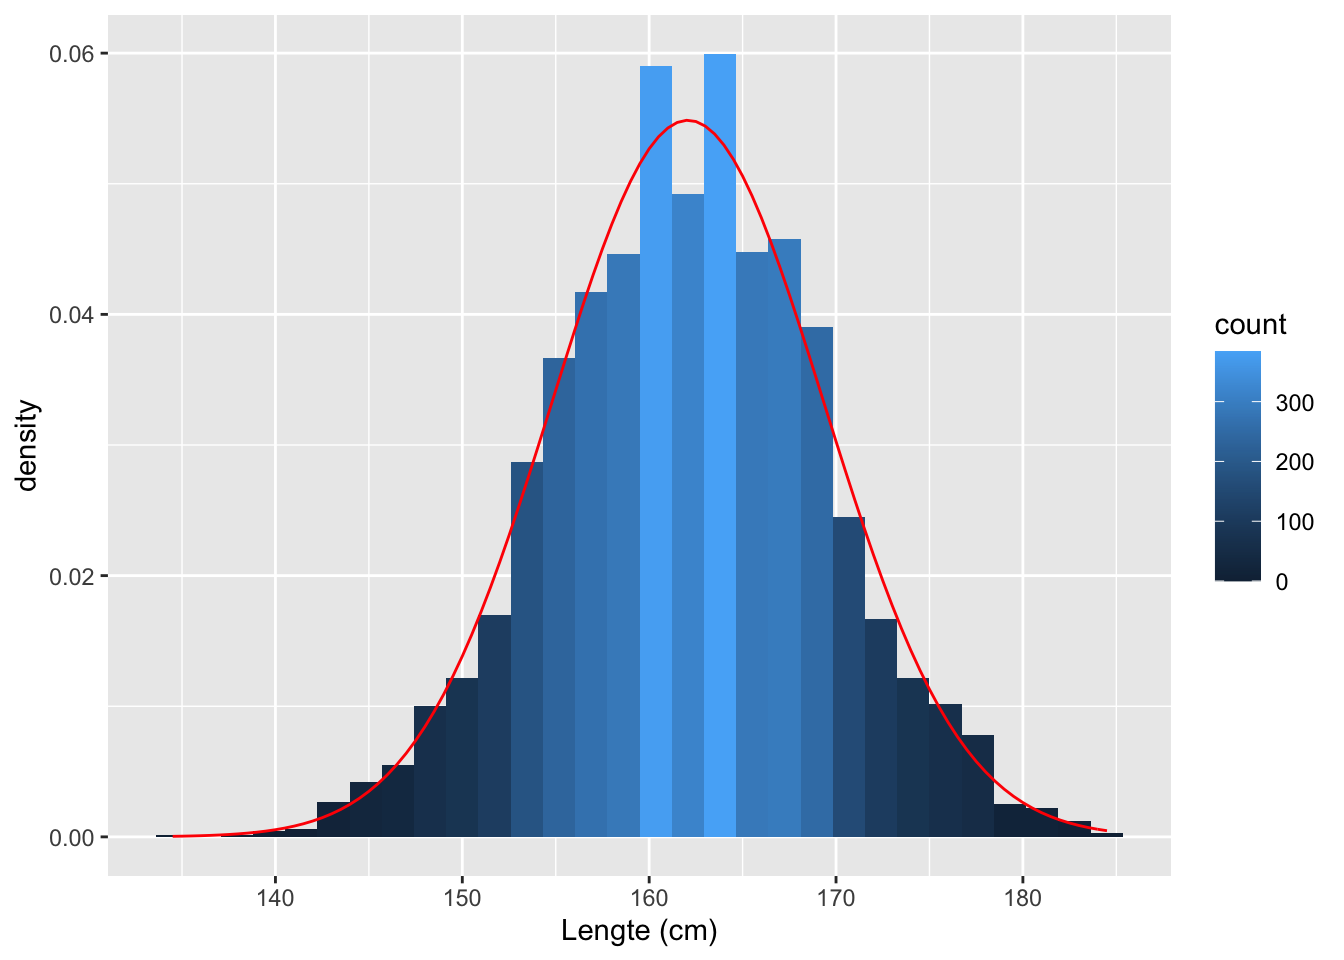
\includegraphics{Statistiek_2020_2021_files/figure-latex/unnamed-chunk-55-1.pdf}

We doen nu hetzelfde op basis van de steekproef met de 10 vrouwen.

\begin{Shaded}
\begin{Highlighting}[]
\NormalTok{HeightSum10 \textless{}{-}}\StringTok{ }\NormalTok{fem10 }\OperatorTok{\%\textgreater{}\%}\StringTok{ }\KeywordTok{summarize}\NormalTok{(}\DataTypeTok{mean =} \KeywordTok{mean}\NormalTok{(Height), }
    \DataTypeTok{sd =} \KeywordTok{sd}\NormalTok{(Height))}

\NormalTok{HeightSum10}
\end{Highlighting}
\end{Shaded}

\begin{verbatim}
## # A tibble: 1 x 2
##    mean    sd
##   <dbl> <dbl>
## 1  163.  8.19
\end{verbatim}

\begin{Shaded}
\begin{Highlighting}[]
\NormalTok{fem10 }\OperatorTok{\%\textgreater{}\%}\StringTok{ }\KeywordTok{ggplot}\NormalTok{(}\KeywordTok{aes}\NormalTok{(}\DataTypeTok{x =}\NormalTok{ Height)) }\OperatorTok{+}\StringTok{ }\KeywordTok{geom\_histogram}\NormalTok{(}\KeywordTok{aes}\NormalTok{(}\DataTypeTok{y =}\NormalTok{ ..density.., }
    \DataTypeTok{fill =}\NormalTok{ ..count..), }\DataTypeTok{bins =} \DecValTok{10}\NormalTok{) }\OperatorTok{+}\StringTok{ }\KeywordTok{xlab}\NormalTok{(}\StringTok{"Lengte (cm)"}\NormalTok{) }\OperatorTok{+}\StringTok{ }
\StringTok{    }\KeywordTok{stat\_function}\NormalTok{(}\DataTypeTok{fun =}\NormalTok{ dnorm, }\DataTypeTok{color =} \StringTok{"red"}\NormalTok{, }\DataTypeTok{args =} \KeywordTok{list}\NormalTok{(}\DataTypeTok{mean =}\NormalTok{ HeightSum10}\OperatorTok{$}\NormalTok{mean[}\DecValTok{1}\NormalTok{], }
        \DataTypeTok{sd =}\NormalTok{ HeightSum10}\OperatorTok{$}\NormalTok{sd[}\DecValTok{1}\NormalTok{])) }\OperatorTok{+}\StringTok{ }\KeywordTok{xlim}\NormalTok{(}\DecValTok{130}\NormalTok{, }\DecValTok{190}\NormalTok{)}
\end{Highlighting}
\end{Shaded}

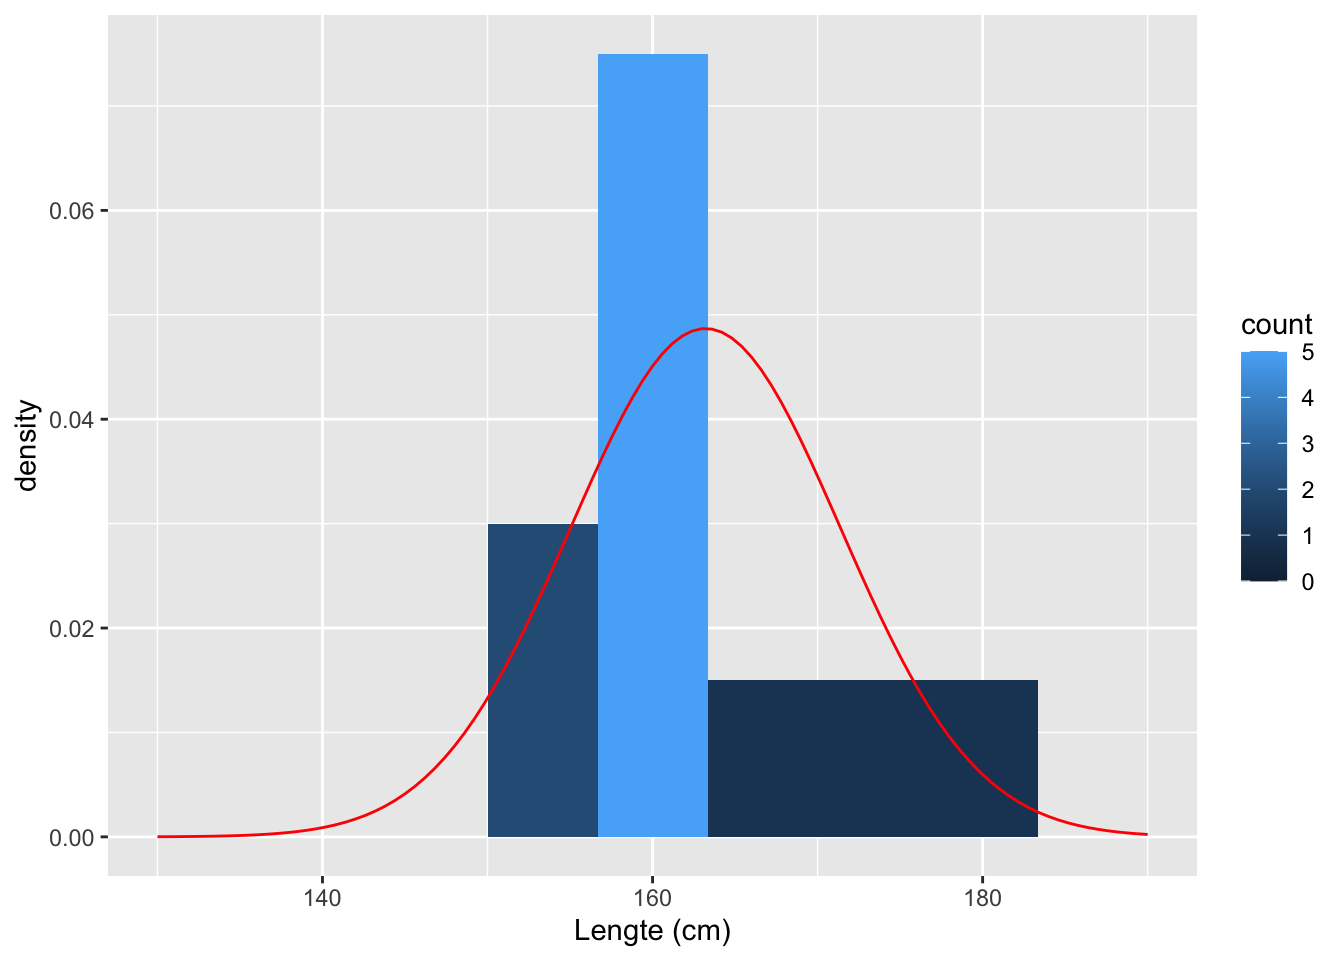
\includegraphics{Statistiek_2020_2021_files/figure-latex/unnamed-chunk-57-1.pdf}

We kunnen de normale benadering nu ook gebruiken om de kans te berekenen dat een vrouw kleiner is dan 150 cm: Pr(X \textless= 150).

We doen dit op basis van de volledige steekproef en vergelijken dit uit wat we bekomen met de ECDF.

\begin{Shaded}
\begin{Highlighting}[]
\KeywordTok{pnorm}\NormalTok{(}\DecValTok{150}\NormalTok{, HeightSum}\OperatorTok{$}\NormalTok{mean[}\DecValTok{1}\NormalTok{], HeightSum}\OperatorTok{$}\NormalTok{sd[}\DecValTok{1}\NormalTok{])}
\end{Highlighting}
\end{Shaded}

\begin{verbatim}
## [1] 0.0484516
\end{verbatim}

\begin{Shaded}
\begin{Highlighting}[]
\KeywordTok{ecdfFem}\NormalTok{(}\DecValTok{150}\NormalTok{)}
\end{Highlighting}
\end{Shaded}

\begin{verbatim}
## [1] 0.05222073
\end{verbatim}

Op basis van de kleine steekproef bekomen we:

\begin{Shaded}
\begin{Highlighting}[]
\KeywordTok{pnorm}\NormalTok{(}\DecValTok{150}\NormalTok{, HeightSum10}\OperatorTok{$}\NormalTok{mean[}\DecValTok{1}\NormalTok{], HeightSum10}\OperatorTok{$}\NormalTok{sd[}\DecValTok{1}\NormalTok{])}
\end{Highlighting}
\end{Shaded}

\begin{verbatim}
## [1] 0.05346615
\end{verbatim}

\begin{Shaded}
\begin{Highlighting}[]
\KeywordTok{ecdfFem10}\NormalTok{(}\DecValTok{150}\NormalTok{)}
\end{Highlighting}
\end{Shaded}

\begin{verbatim}
## [1] 0
\end{verbatim}

Voor kleine steekproef is geschatte kans o.b.v. empirische distributie veel minder nauwkeurig.
Kwantielen geschat o.b.v. kleine steekproef zijn immers vrij onzeker. Ze gebruiken immers maar een fractie van de data.\\
De schatting o.b.v. de normale verdeling laat toe om alle data te gebruiken voor het schatten van de model parameters en is daarom nauwkeuriger. Uiteraard heeft de laatste aanpak de beperking dat de data Normaal verdeeld moeten zijn.

\hypertarget{referentie-intervallen}{%
\subsection{Referentie intervallen}\label{referentie-intervallen}}

Het bepalen van grenswaarden voor de lengte die vrij veel voorkomen kunnen worden bekomen door gebruik te maken van een referentie interval.

Typisch wordt een 95\% referentie interval gebruikt zodat we voor 95\% van de subjecten in de populatie verwachten dat ze een karakteristiek hebben die in het referentie interval ligt.

We kunnen dat opnieuw op basis van de empirische distributie.

\begin{itemize}
\item
  We moeten hiervoor \(\hat{F}(x_{2.5\%})=0.025\) en \(\hat{F}(x_{97.5\%})=0.975\) berekenen zodat 95\% van de observaties in de steekproef vallen in het interval \([x_{2.5\%},x_{97.5\%}]\).
\item
  Dat kan met de \texttt{quantile} functie.
\end{itemize}

Grote steekproef

\begin{Shaded}
\begin{Highlighting}[]
\NormalTok{NHANES }\OperatorTok{\%\textgreater{}\%}\StringTok{ }\KeywordTok{filter}\NormalTok{(Gender }\OperatorTok{==}\StringTok{ "female"} \OperatorTok{\&}\StringTok{ }\OperatorTok{!}\KeywordTok{is.na}\NormalTok{(Height) }\OperatorTok{\&}\StringTok{ }
\StringTok{    }\NormalTok{Age }\OperatorTok{\textgreater{}}\StringTok{ }\DecValTok{18}\NormalTok{) }\OperatorTok{\%\textgreater{}\%}\StringTok{ }\KeywordTok{pull}\NormalTok{(Height) }\OperatorTok{\%\textgreater{}\%}\StringTok{ }\KeywordTok{quantile}\NormalTok{(}\DataTypeTok{prob =} \KeywordTok{c}\NormalTok{(}\FloatTok{0.025}\NormalTok{, }
    \FloatTok{0.975}\NormalTok{))}
\end{Highlighting}
\end{Shaded}

\begin{verbatim}
##  2.5% 97.5% 
## 147.6 176.7
\end{verbatim}

\begin{itemize}
\tightlist
\item
  Op basis van de grote steekproef schatten we dat 95\% van de vrouwen in de populatie een lengte heeft die ligt in het interval {[}147.6, 176.7{]}.
\end{itemize}

Kleine steekproef

\begin{Shaded}
\begin{Highlighting}[]
\NormalTok{fem10 }\OperatorTok{\%\textgreater{}\%}\StringTok{ }\KeywordTok{pull}\NormalTok{(Height) }\OperatorTok{\%\textgreater{}\%}\StringTok{ }\KeywordTok{quantile}\NormalTok{(}\DataTypeTok{prob =} \KeywordTok{c}\NormalTok{(}\FloatTok{0.025}\NormalTok{, }
    \FloatTok{0.975}\NormalTok{))}
\end{Highlighting}
\end{Shaded}

\begin{verbatim}
##     2.5%    97.5% 
## 154.7250 178.3275
\end{verbatim}

\begin{itemize}
\tightlist
\item
  Dit interval o.b.v. de kleine steekproef is een ruwe benadering.
\item
  We hebben immers niet voldoende observaties om een goede benadering te hebben voor extreme quantielen.
\end{itemize}

\hypertarget{normale-benadering-1}{%
\subsubsection{Normale benadering}\label{normale-benadering-1}}

We kunnen de functie qnorm gebruiken om quantielen te berekenen van de normale distributie. We weten dat een 95\% referentie interval ongeveer binnen twee standaard deviaties rond het gemiddelde ligt.

We doen dit nu voor de
- Grote steekproef

\begin{Shaded}
\begin{Highlighting}[]
\KeywordTok{qnorm}\NormalTok{(}\FloatTok{0.025}\NormalTok{, }\DataTypeTok{mean =}\NormalTok{ HeightSum}\OperatorTok{$}\NormalTok{mean, }\DataTypeTok{sd =}\NormalTok{ HeightSum}\OperatorTok{$}\NormalTok{sd)}
\end{Highlighting}
\end{Shaded}

\begin{verbatim}
## [1] 147.8192
\end{verbatim}

\begin{Shaded}
\begin{Highlighting}[]
\NormalTok{HeightSum}\OperatorTok{$}\NormalTok{mean }\OperatorTok{{-}}\StringTok{ }\DecValTok{2} \OperatorTok{*}\StringTok{ }\NormalTok{HeightSum}\OperatorTok{$}\NormalTok{sd}
\end{Highlighting}
\end{Shaded}

\begin{verbatim}
## [1] 147.528
\end{verbatim}

\begin{Shaded}
\begin{Highlighting}[]
\KeywordTok{qnorm}\NormalTok{(}\FloatTok{0.975}\NormalTok{, }\DataTypeTok{mean =}\NormalTok{ HeightSum}\OperatorTok{$}\NormalTok{mean, }\DataTypeTok{sd =}\NormalTok{ HeightSum}\OperatorTok{$}\NormalTok{sd)}
\end{Highlighting}
\end{Shaded}

\begin{verbatim}
## [1] 176.3237
\end{verbatim}

\begin{Shaded}
\begin{Highlighting}[]
\NormalTok{HeightSum}\OperatorTok{$}\NormalTok{mean }\OperatorTok{+}\StringTok{ }\DecValTok{2} \OperatorTok{*}\StringTok{ }\NormalTok{HeightSum}\OperatorTok{$}\NormalTok{sd}
\end{Highlighting}
\end{Shaded}

\begin{verbatim}
## [1] 176.6149
\end{verbatim}

\begin{itemize}
\tightlist
\item
  Kleine steekproef
\end{itemize}

\begin{Shaded}
\begin{Highlighting}[]
\KeywordTok{qnorm}\NormalTok{(}\FloatTok{0.025}\NormalTok{, }\DataTypeTok{mean =}\NormalTok{ HeightSum10}\OperatorTok{$}\NormalTok{mean, }\DataTypeTok{sd =}\NormalTok{ HeightSum10}\OperatorTok{$}\NormalTok{sd)}
\end{Highlighting}
\end{Shaded}

\begin{verbatim}
## [1] 147.1499
\end{verbatim}

\begin{Shaded}
\begin{Highlighting}[]
\KeywordTok{qnorm}\NormalTok{(}\FloatTok{0.975}\NormalTok{, }\DataTypeTok{mean =}\NormalTok{ HeightSum10}\OperatorTok{$}\NormalTok{mean, }\DataTypeTok{sd =}\NormalTok{ HeightSum10}\OperatorTok{$}\NormalTok{sd)}
\end{Highlighting}
\end{Shaded}

\begin{verbatim}
## [1] 179.2701
\end{verbatim}

We zien dat de benadering voor de kleine steekproef op basis van de aanname van Normaliteit opnieuw goed werkt!

\hypertarget{conclusions}{%
\subsection{Conclusions}\label{conclusions}}

\begin{itemize}
\item
  Voor de grote steekproef geven de empirische distributie en de normale benadering vergelijkbare resultaten.
\item
  Voor de kleine steekproef werkt de normale benadering beter dan de empirische distributie.

  \begin{itemize}
  \tightlist
  \item
    We kijken immers naar extreme quantielen 2.5\% en 97.5\%.
  \item
    Er zijn inderdaad weinig gegevens in de steekproef die toelaten om deze quantielen direct te schatten.
  \item
    Met de normale benadering kunnen we alle data gebruiken om het gemiddelde en de standaarddeviatie te schatten.
  \item
    Als de aanname van normaliteit geldt dan krijgen we betere schattingen voor deze kwantielen.
  \end{itemize}
\end{itemize}

\hypertarget{statistieken}{%
\section{Statistieken}\label{statistieken}}

Formules die gebruikt worden om parameters van de verdeling in de populatie te schatten op basis van de
steekproef, alsook het numerieke resultaat dat men bekomt door deze formules
te evalueren, worden \emph{statistieken} genoemd.
Bijvoorbeeld het
rekenkundig gemiddelde van alle systolische bloeddrukwaarden voor de verschillende subjecten
in de steekproef, is een statistiek. Statistieken zijn dus wat
de onderzoekers observeren of kunnen berekenen o.b.v. de gegevens in de
steekproef; parameters zijn wat ze eigenlijk willen weten.
Omdat statistieken berekend worden op basis van de gegevens uit de steekproef, zullen ze variëren van steekproef tot steekproef.
We zullen ze daarom noteren met een hoofdletter (bvb. \(\bar X\) voor het steekproefgemiddelde), tenzij we verwijzen naar de numerieke waarde die gerealiseerd wordt in een bepaalde steekproef, in welk geval we een kleine letter gebruiken (bvb. \(\bar x\) voor het steekproefgemiddelde).

\hypertarget{conventie}{%
\section{Conventie}\label{conventie}}

\textbf{Belangrijke Conventie:} In de cursus gebruiken we de conventie om \textbf{populatieparameters die een vaste waarden aannemen maar die meestal ongekend zijn} voor te stellen door \textbf{Griekse symbolen}. \textbf{Statistieken} waarmee we deze ongekende parameters schatten o.b.v. een steekproef zullen we weergeven door \textbf{letters}.

Voor de normaal verdeling hebben we dus:

\begin{longtable}[]{@{}cc@{}}
\toprule
Populatie & Steekproef\tabularnewline
\midrule
\endhead
\(\mu\) & \(\bar X\)\tabularnewline
\(\sigma^2\) & \(S^2\)\tabularnewline
\bottomrule
\end{longtable}

Om hetgeen we in de steekproef observeren te kunnen veralgemenen naar de populatie, zullen we gebruik moeten maken van methodes uit de statistische besluitvorming wat in latere hoofdstukken aan bod komt.

De cursus is als volgt georganiseerd:
In hoofdstuk \ref{chap:design} verdiepen we ons in studiedesign. Vervolgens gaan we in op data-exploratie in hoofdstuk \ref{chap:describe}, hierbij zullen we de gegevens in een steekproef grondig exploreren zodoende inzicht te verwerven in de data en hoe we ze statistisch kunnen modelleren.
In hoofdstuk \ref{chap:besluit} introduceren we de grondslagen van statistische besluitvorming die het ons mogelijk maakt om effecten die we observeren in de steekproef te kunnen veralgemenen naar de populatie toe.
In hoofdstukken \ref{chap:linReg}-\ref{chap:glm} zullen we meer geavanceerde statistische modellen en methoden introduceren om data te modelleren en voor statistische besluitvorming.

\hypertarget{code-voor-dit-hoofdstuk}{%
\section{Code voor dit hoofdstuk}\label{code-voor-dit-hoofdstuk}}

\begin{enumerate}
\def\labelenumi{\arabic{enumi}.}
\tightlist
\item
  Continue Toevallige Veranderlijken:
\end{enumerate}

\begin{enumerate}
\def\labelenumi{\arabic{enumi}.}
\setcounter{enumi}{1}
\tightlist
\item
  Lengte voorbeeld:
\end{enumerate}

\hypertarget{chap:design}{%
\chapter{Studiedesign}\label{chap:design}}

Alle kennisclips die in dit hoofdstuk zijn verwerkt kan je in deze youtube playlist vinden: \href{https://www.youtube.com/playlist?list=PLZH1hP8_LbJL1GjhnpEDlx78OJ6qUzSix}{Kennisclips Hoofdstuk3}

\hypertarget{inleiding}{%
\section{Inleiding}\label{inleiding}}

Centraal in wetenschappelijk onderzoek is de wens en noodzaak om
theorie-gebaseerde kennis empirisch (d.w.z. door middel van observatie) te
verifiëren en op te bouwen. Terwijl theorie-gebaseerde kennis voortvloeit uit hypothesen
omtrent het bestudeerde biologische of chemische proces, ontstaat empirische
kennis door lukraak subjecten (mensen, planten, dieren) uit een doelpopulatie te
trekken volgens een gestructureerd schema en hen vervolgens te observeren.
Dit gestructureerde schema, dat ondermeer vastlegt welke en hoeveel
subjecten in de studie worden opgenomen en eventueel wie welke experimentele
interventie zal ondergaan, noemt men het \emph{design} van de studie of de
\emph{proefopzet}. Met een goed design kunnen betrouwbare conclusies
worden getrokken op basis van de gegevens. Het bepaalt immers welke
informatie wel en niet in de dataset vervat zal zijn. Fouten bij het design
van een studie kunnen soms gecorrigeerd worden door de statistische analyse,
maar zijn helaas vaak onherroepelijk. Het design is daarom van cruciaal
belang voor een studie en vereist evenveel aandacht als de uiteindelijke
statistische analyse van de observaties. Ook in deze cursus vormen de
concepten in dit hoofdstuk rond design wellicht het meest
belangrijke onderwerp, hoewel we er slechts beknopt op in kunnen gaan. De
ideeën lijken eenvoudig, maar dat is vaak een bedrieglijke indruk!

\begin{figure}

{\centering 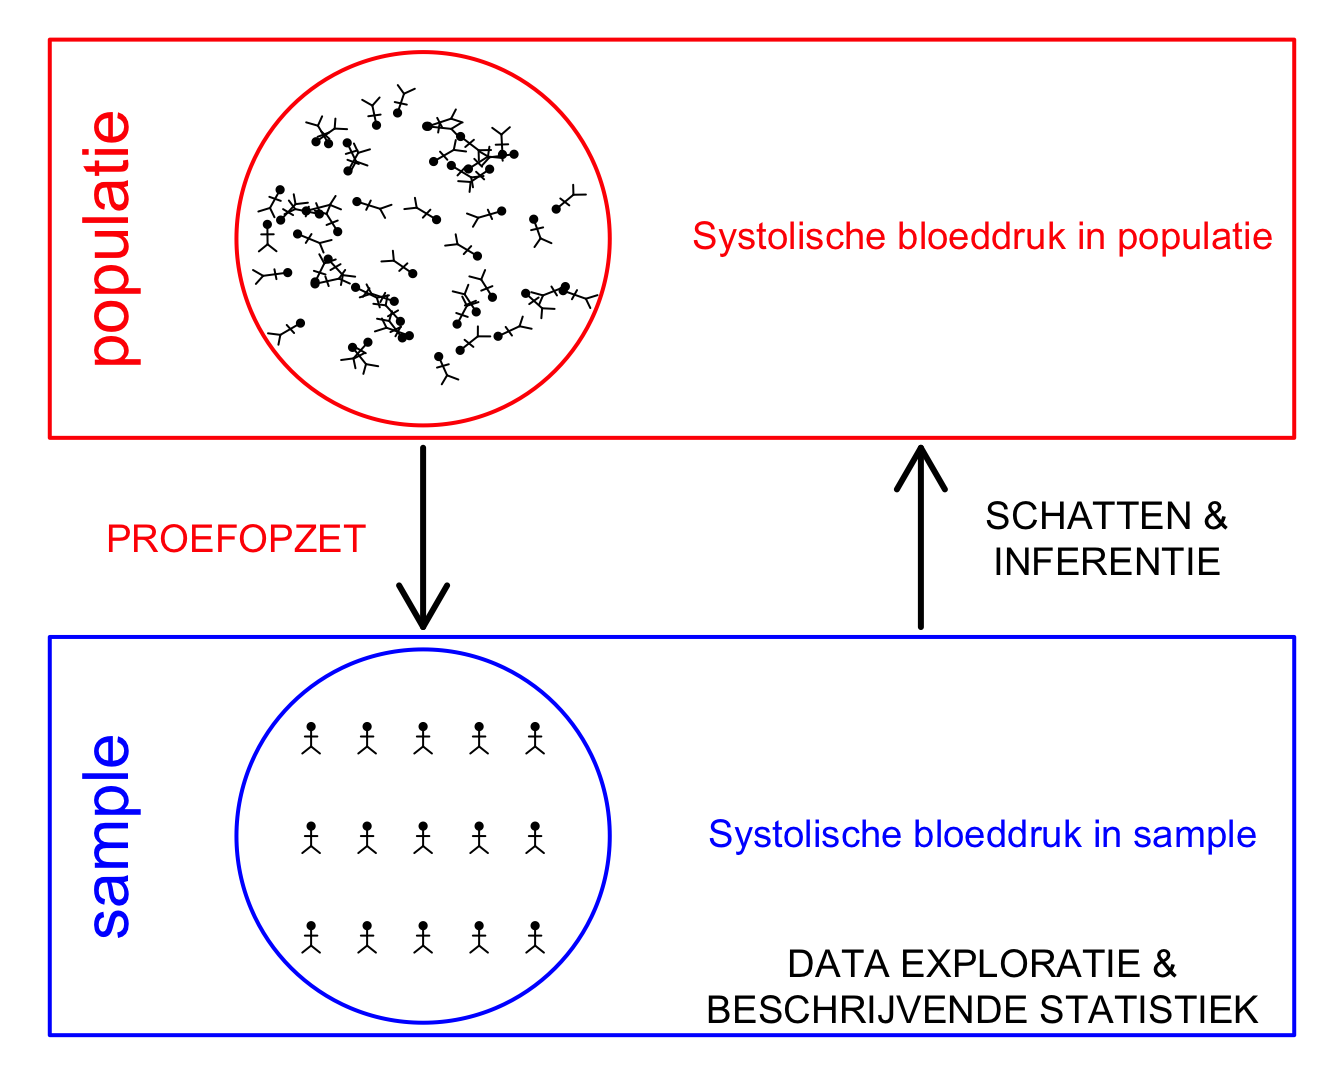
\includegraphics[width=1\linewidth]{Statistiek_2020_2021_files/figure-latex/pop2Samp2PopDesign-1} 

}

\caption{Verschillende stappen in een studie. In dit hoofdstuk ligt de focus op proefopzet.}\label{fig:pop2Samp2PopDesign}
\end{figure}

\hypertarget{sec:steekproefdesigns}{%
\section{Steekproefdesigns}\label{sec:steekproefdesigns}}

In de praktijk vestigt men de interesse van een onderzoek op een bepaalde biologische \emph{populatie}. Vervolgens zal men een geschikt type en grootte van monsters of stalen (of meer algemeen experimentele eenheden en/of subjecten genoemd doorheen deze cursus) definiëren waarvoor men metingen zal verzamelen. Bijvoorbeeld, indien men de grootte van de populatie salamanders van de species Plethodon jordani wenst te bestuderen, kan men de aandacht van het onderzoek vestigen op de bestaande populatie P. jordani in de Great Smoky Mountains (d.i. de populatie) en vervolgens het aantal salamanders tellen op oppervlakte-eenheden van 10 m\(^2\) (die eenheden zijn de stalen of ``experimentele eenheden''; voor elke experimentele eenheid bekomt men aldus een meting). Indien men de impact van roofvissen op zeebodemhabitats wenst te evalueren, dan kan het onderzoek de aandacht vestigen op de zeebodem binnen een afstand van 500 m voor de Belgische Noordzeekust (d.i. de biologische populatie) en kunnen vervolgens metingen worden verzameld op stukjes zeebodem met een straal van 1 m (d.i. de ``stalen'' in de studie). Omdat het in de praktijk bijna nooit mogelijk is om de hele populatie te onderzoeken (alle salamanders in de Great Smoky Mountains, de ganse zeebodem binnen een afstand van 500 m voor de Belgische Noordzeekust), zal men zich beperken tot gegevens voor een zogenaamde \emph{steekproef}, een beperkte verzameling stalen, experimentele eenheden of subjecten uit de populatie.

Welke subjecten uit de populatie men precies zal bestuderen, zal uiteraard zijn weerslag hebben op de resultaten van de uiteindelijke analyse van de gegevens. Opdat de resultaten die men observeert voor de steekproef veralgemeenbaar zouden zijn naar de ganse studiepopulatie, is het noodzakelijk dat men de subjecten uit de steekproef zodanig kiest dat ze representatief zijn voor de populatie. De basismethode om dat te realiseren, heet \emph{eenvoudige lukrake steekproeftrekking} (in het Engels: \emph{simple random sampling}). Ze bestaat erin te garanderen dat elk subject in de populatie een zelfde kans heeft om in de steekproef terecht te komen. Zo kan men bijvoorbeeld elke muis in een kooi een nummer geven en vervolgens lukraak een aantal \(n\) van die nummers trekken. In de praktijk, en in het bijzonder in de veldbiologie, is die methode echter vaak moeilijk toe te passen omdat de subjecten in de populatie bijvoorbeeld geen goed onderscheiden habitats vormen, niet op voorhand genummerd kunnen worden of omdat de populatie een te groot gebied bestrijkt. Zo is het bijvoorbeeld niet makkelijk om een eenvoudige lukrake steekproef van salamanders in de Great Smoky Mountains te bekomen omdat het bestudeerde gebied zeer groot is en de salamanders uiteraard niet genummerd kunnen worden. In die gevallen gaan biologen vaak over op \emph{haphazard sampling}, waarbij men op een minder formele manier stalen verzamelt, maar er toch voor probeert te zorgen dat de resultaten niet vertekend worden doordat bepaalde subjecten meer kans hebben om in de steekproef terecht te komen. Bijvoorbeeld kan men een computer lukraak plaatsen laten aanduiden in de Great Smoky Mountains en kan men vervolgens metingen proberen te verzamelen voor de eerste salamander die telkens in de buurt van de aangeduide plaatsen voorbijkomt.

Sommige steekproefdesigns houden expliciet rekening met heterogeniteit in de populatie waaruit een steekproef wordt genomen. Bij \emph{gestratificeerde lukrake steekproeven} (in het Engels: \emph{stratified random samples}) wordt de populatie opgedeeld in verschillende strata, die goed onderscheiden subgroepen in de populatie identificeren, en worden vervolgens eenvoudige lukrake steekproeven uit elk stratum genomen. Stel bijvoorbeeld dat men karakteristieken van stenen in een rivier wenst te beschrijven en dat stenen in verschillende habitats voorkomen (rotsige, ondiepe waters, diepe waters, stille binnenwaters,\ldots), dan kan het zinvol zijn om een gestratificeerde lukrake steekproef te nemen om ervoor te zorgen dat er binnen elk stratum (d.i. elke habitat) een voldoende aantal stenen verzameld worden.

Bij \emph{geclusterde steekproeftrekking} (in het Engels: \emph{cluster sampling}) worden clusters van meer verwante subjecten uit de populatie getrokken. Stel bijvoorbeeld dat we de impact van verschillende vormen van beschadiging aan bladeren van een boom wensen te meten, dan kunnen we in een eerste fase een eenvoudige lukrake steekproef van bomen bepalen. Vervolgens kunnen we in een tweede fase binnen elke boom een eenvoudige lukrake steekproef van bladeren bepalen en de verschillende gekozen bladeren aan verschillende vormen van beschadiging onderwerpen. Dit noemt men (two stage) cluster sampling omdat bladeren afkomstig van een zelfde boom meer verwant en bijgevolg geclusterd zijn. We zullen later zien dat men in de analyse van gegevens uit dergelijke studie met die clustering rekening moet houden.

Tenslotte steunt men in de biologische wetenschappen ook vaak op \emph{systematische steekproeven} waarbij men bijvoorbeeld monsters neemt die op vaste afstand van elkaar bekomen worden of op voorafgekozen tijdstippen, en om die reden niet volledig lukraak genoemd kunnen worden. Dit wordt vaak gebruikt wanneer men een omgevings- of tijdsgradiënt wenst te beschrijven voor een bepaald proces, zoals de wijziging in rijkdom aan species naarmate men zich verwijdert van een vervuilingsbron. Dergelijke designs zijn nuttig en logistiek zeer praktisch, maar kunnen vertekende resultaten opleveren wanneer de monsters op specifieke plaatsen genomen worden die samenvallen met een ongekende omgevings- of tijdsgradiënt (d.i. indien de gekozen plaatsen selectief zijn en afwijkend van de globale omgevings- of tijdsgradiënt).

\hypertarget{replicatie}{%
\subsection{Replicatie}\label{replicatie}}

Replicatie betekent dat herhaaldelijke observaties worden bekomen, op verschillende plaatsen, voor verschillende dieren of planten, op verschillende tijdstippen, \ldots{} Dergelijke herhalingen zijn essentieel in empirisch onderzoek omdat biologische en ecologische systemen vaak zeer variabel zijn en de beschikbaarheid van meerdere observaties toelaat om ruis op de gegevens te drukken. Hoewel biologen, biotechnologen en biochemici zich goed bewust zijn van de nood voor replicatie wordt vaak misbegrepen op welke schaal die herhalingen moeten bekomen worden. Wellicht is er geen enkel aspect van studiedesign dat meer verwarring veroorzaakt bij wetenschappers dan dit. Stel bijvoorbeeld dat men een studie wenst op te zetten om het effect van bosbranden op de rijkdom aan ongewervelde dieren te onderzoeken. Meestal zal men dan gebruik maken van natuurlijke bosbranden. Stel dat 1 verbrand gebied gelocaliseerd wordt en vergeleken wordt met een naburig gebied waar geen bosbrand plaatsvond. Stel verder dat men binnen elk gebied verschillende stalen bodemkorst neemt om de rijkdom aan ongewervelden te bepalen. Dan beschikt men wel over herhaaldelijke metingen (namelijk verschillende stukken bodemkorst per gebied), maar niet op de juiste schaal. De metingen voor de rijkdom aan species die men uit het verbrande gebied bekomen heeft, meten immers de impact van dezelfde brand. Als gevolg daarvan kan men op basis van eventuele verschillen in species rijkdom tussen beide gebieden niet bepalen of ze het gevolg zijn van de brand dan wel van andere verschillen tussen beide gebieden die eveneens een impact op ongewervelden hebben. Uit dergelijke vergelijking kan men hoogstens besluiten dat de gebieden al dan niet verschillen, maar niet waardoor ze verschillen.

De herhaalde stukken bodemkorst in bovenstaand voorbeeld stellen substeekproeven voor. Deze stellen geen herhalingen voor van de bestudeerde interventie (bosbranden) en worden daarom pseudoreplicaties genoemd. Pseudoreplicaties zijn nuttig omdat ze replicaties zijn (op een zeker niveau) en daardoor toelaten om een deel van de ruis op de gegevens weg te middelen. In sommige studies zijn echte replicaties onmogelijk en is het bijgevolg onvermijdelijk om zijn toevlucht tot pseudoreplicaties te nemen. Bijvoorbeeld, indien men een experiment uitvoert dat kamers van constante temperatuur vereist, dan kan het best zijn dat er binnen een gegeven instituut slechts een tweetal dergelijke kamers beschikbaar zijn omwille van hun hoge kost. Indien men bijvoorbeeld de impact wenst te onderzoeken van rioollozing op de biomassa van phytoplankton in een bepaalde kuststreek, dan is er vaak maar 1 riool waarin men echt geïnteresseerd is, terwijl het aantal naburige lokaties zonder riool zeer uitgebreid kan zijn. In dat geval zal men vaak stalen nemen op meerdere plaatsen zonder riool om in ieder geval de variatie tussen controlesites (d.i. sites zonder rioollozing) te minimaliseren. \emph{Before-After-Control-Impact (BACI) designs} proberen verder informatie te winnen door zowel metingen te nemen vóór de interventie (bvb. het plaatsen van een riool) als na de interventie.

\hypertarget{experimentele-studies}{%
\section{Experimentele studies}\label{experimentele-studies}}

Studiedesigns worden opgesplits in \emph{experimentele studies of experimenten} waar de onderzoeker eerst het biologische systeem manipuleert en vervolgens observeert, en \emph{observationele studies} waar de onderzoeker enkel observeert zonder zelf in het systeem in te grijpen. In deze sectie gaan we dieper in op het eerste type studies. Observationele studies worden besproken in Sectie \ref{sec:observational}.

\begin{definition}[experiment]
\begin{definition}

\protect\hypertarget{def:unnamed-chunk-64}{}{\label{def:unnamed-chunk-64} \iffalse (experiment) \fi{} }

\end{definition}
\end{definition}

Een \textbf{experiment} is een reeks observaties die gemaakt worden onder
condities die gecontroleerd worden door de onderzoeker. De onderzoeker
controleert hierbij verschillende factoren (zoals de keuze van de
interventie voor een locatie, plant, dier), met als doel een zuiver antwoord op de gestelde onderzoeksvraag te bepalen.
\footnote{Met ``zuiver'' wordt hier bedoeld dat de het zuivere interventie-effect uit de gegevens
  kan gehaald worden zonder dat het antwoord wordt beïnvloed door andere aspecten/variabelen. Dit wordt meer concreet in Hoofdstuk \{chap:sample\}
  uitgelegd. Voorlopig volstaat de intuïtieve betekenis van het woord.}

\textbf{Einde definitie}

Bijvoorbeeld, wanneer een dierenfysioloog 2 behandelingen wenst te vergelijken tussen experimentele dieren,
dan kan hij - zoals we in dit hoofdstuk zullen zien - vermijden dat het
behandelingseffect vertekend\footnote{ Voorlopig verstaan we onder het feit dat een schatting voor het
  behandelingseffect `vertekend' is, dat het foutief werd ingeschat of, m.a.w., dat het geschatte effect niet correct het zuivere effect van de behandeling weerspiegelt. Een meer concrete definitie volgt eveneens in
  Hoofdstuk \{chap:sample\}.} is door vergelijkbare groepen dieren te creëren;
bijvoorbeeld, door lukraak (bijvoorbeeld door
het opgooien van een muntstuk) te bepalen welke behandeling aan welk
dier wordt toegediend.

\hypertarget{de-salk-vaccin-veldstudie}{%
\subsection{De Salk Vaccin Veldstudie}\label{de-salk-vaccin-veldstudie}}

Om de basisprincipes van experimentele designs in te voeren, gebruiken we als rode draad de Salk Vaccin Veldstudie. Vooraleer dieper op deze studie in te gaan, schetsen we de historische context.

De eerste polio-epidemie in de Verenigde Staten brak uit in 1916 en kostte
aan honderdduizenden mensen, vooral kinderen, het leven. Tegen de jaren 1950
waren er verschillende vaccins ontwikkeld. Vooral het vaccin dat door John
Salk werd ontwikkeld, leek veelbelovend omdat het zich veilig en effectief
had getoond in laboratoriumstudies. In 1954 werd door de National Foundation
for Infantile Paralysis (NFIP) een grote studie opgezet om de effectiviteit
van het vaccin buiten het laboratorium na te gaan. Meer concreet wenstte men
na te gaan wat de invloed was van vaccinatie op de polio-incidentie.

\begin{definition}[incidentie en prevalentie]
\begin{definition}

\protect\hypertarget{def:unnamed-chunk-65}{}{\label{def:unnamed-chunk-65} \iffalse (incidentie en prevalentie) \fi{} }

\end{definition}
\end{definition}

De \textbf{incidentie} van een bepaalde ziekte of aandoening (bvb. polio)
wordt gedefinieerd als het verwachte aantal nieuwe gevallen van die ziekte
dat optreedt gedurende een vooraf bepaald tijdsinterval, uitgedrukt per
eenheid van een ziektevrije populatie. Het drukt m.a.w. de kans uit dat een
individu zonder de bestudeerde aandoening tijdens het gegeven tijdsinterval
deze aandoening zal opdoen.

De \textbf{prevalentie} van een bepaalde ziekte wordt gedefinieerd als de
proportie individuen met de ziekte in een bepaalde populatie op een bepaald
punt in de tijd.

\textbf{Einde definitie}

Stel dat de NFIP het vaccin gewoon had toegediend aan een groot aantal
kinderen en dat ze een daling observeerden in de incidentie van polio van
1953 naar 1954. Dit betekent dat de kans dat een lukraak polio-vrij kind een
polio-infectie opdeed in de loop van 1954 (d.i. de incidentie van polio in
1954), lager is dan de kans dat lukraak polio-vrij kind een polio-infectie
opdoet in de loop van 1953 (d.i. de incidentie van polio in 1953). In dat
geval kan men niet zomaar besluiten dat het vaccin effectief is. Immers,
afgezien van de introductie van een vaccin, varieert de incidentie van polio
van jaar tot jaar. Zo zou men, indien het vaccin niet effectief was, toch
een daling in polio-incidentie van 1953 naar 1954 kunnen vaststellen in
geval 1954 geen epidemisch jaar zou zijn.

De enige manier om te ontdekken of het vaccin effectief is, is om \emph{gelijktijdig} de incidentie van polio in 1954 te vergelijken tussen een
groep gevaccineerde kinderen (doorgaans \emph{cases} genoemd) en een groep
niet-gevaccineerde kinderen (doorgaans \emph{controles} genoemd). Dit is
wat de NFIP heeft gedaan. De deelnemers aan de studie waren kinderen uit de
leeftijdsgroepen die het meest vatbaar waren voor polio. De studie verliep in
verschillende schooldistricten in de Verenigde Staten waar het risico op
polio hoog was. Aan ongeveer 350000 kinderen uit de tweede graad werd
vaccinatie voorgeschreven. Voor 125000 van hen weigerden de ouders
toestemming te geven om deze vaccinatie te laten doorgaan, zodat de groep
cases uiteindelijk uit de overige 225000 kinderen bestond. Ongeveer
750000 kinderen uit de eerste en derde graad werden vrijwillig niet
gevaccineerd; zij vormden de controles.

Het feit dat de groep cases en de groep controles een verschillende grootte
hebben is niet problematisch zolang men niet het absolute aantal, maar het
percentage polio-besmettingen tussen beide groepen vergelijkt. Toch hoeft
een geobserveerd verschil in incidentie tussen gevaccineerde en
niet-gevaccineerde kinderen nog steeds niet noodzakelijk te impliceren dat
het vaccin effectief is. Hier zijn verschillende redenen voor:

\begin{enumerate}
\def\labelenumi{\arabic{enumi}.}
\tightlist
\item
  Ten eerste zou het kunnen dat men door toeval een verschil in
  incidentie waarneemt tussen beide groepen, doordat er per toeval
  bijvoorbeeld relatief gezien minder kinderen in de gevaccineerde groep polio
  ontwikkelen. In Hoofdstuk \ref{chap:besluit} zullen we methoden aanleren om
  uit te maken of een geobserveerd vaccinatie-effect (d.w.z. een
  vaccinatie-effect dat geschat of berekend werd o.b.v. de gegevens) al dan
  niet toevallig is.
\item
  Ten tweede zou het kunnen dat kinderen uit de tweede graad sowieso
  meer vatbaar zijn voor polio en er, afgezien van het werkelijke
  vaccin-effect, voor de cases dus een hogere incidentie wordt verwacht.
\item
  Ten derde is het zo dat vooral ouders uit hoge-inkomens gezinnen
  geneigd waren om de toestemming te geven hun kind te laten vaccineren, zodat
  de groep cases hoofdzakelijk bestaat uit kinderen van hoge-inkomens
  gezinnen. Deze kinderen zijn meer vatbaar voor polio omdat ze, wegens de
  betere hygiënische omstandigheden in deze gezinnen, minder antilichamen
  tegen polio ontwikkeld hebben.
\end{enumerate}

Het geobserveerde verschil in incidentie tussen gevaccineerde en
niet-gevaccineerde kinderen weerspiegelt daarom niet alleen de effectiviteit
van het vaccin, maar ook het feit dat kinderen uit graad 2 mogelijks niet
vergelijkbaar zijn met de resterende kinderen en het feit dat cases, omwille
van betere hygiënische omstandigheden, meer vatbaar zijn voor polio dan
controles. In het bijzonder is het om die reden mogelijk om, zelfs als het
vaccin effectief is, een gelijke incidentie voor cases en controles vast te
stellen. In dat geval verwart men het effect van het vaccin met het feit dat
cases meer vatbaar zijn voor polio dan controles.

De statistische les die we hier algemeen uit kunnen trekken, is dat de
verschillende interventiegroepen zo vergelijkbaar mogelijk moeten zijn bij
de bepaling van het effect van een interventie, opdat elk verschil in respons tussen
de groepen volledig kan toegeschreven worden aan de verschillende
interventie. Wanneer de groepen cases en controles niet volledig
vergelijkbaar zijn in een bepaalde factor (zoals de vatbaarheid voor polio,
maar niet de interventie zelf), dan is het mogelijk dat het effect van die
factor verward (in het Engels: \emph{confounded}) wordt met het effect van
de interventie. Men noemt die factor dan een confounder voor het effect van
de interventie. De belangrijkste beperking op de ondubbelzinnige interpretatie van studieresultaten is het probleem van confounding.

\begin{example}[De nood aan controle]
\begin{example}

\protect\hypertarget{exm:unnamed-chunk-66}{}{\label{exm:unnamed-chunk-66} \iffalse (De nood aan controle) \fi{} }

\end{example}
\end{example}

Hairston (1980) bestudeerde de stelling dat 2 soorten salamander (P. jordani en P. glutinosus) in de Great Smoky Mountains mekaar rivaliseren. Hij zette daartoe experimenten op waarbij P. glutinosus verwijderd werd van bepaalde territoria. De populatie van P. jordani begon toe te nemen in de 3 jaren die volgden op de verwijdering van de salamanders, maar nam al even sterk toe op controleterritoria waar P. glutinosus niet verwijderd was. Had Hairston geen controleterritoria onderzocht, dan had hij mogelijks de toename in de populatie van P. jordani verkeerdelijk toegeschreven aan het verwijderen van P. glutinosus.

\textbf{Einde voorbeeld}

\begin{definition}[confounding en confounder]
\begin{definition}

\protect\hypertarget{def:unnamed-chunk-67}{}{\label{def:unnamed-chunk-67} \iffalse (confounding en confounder) \fi{} }

\end{definition}
\end{definition}

\textbf{Confounding} is het probleem dat verschillen ten gevolge van verschillende experimentele interventies niet kunnen losgekoppeld worden van andere factoren, \textbf{confounders} genoemd, die verschillen tussen de interventiegroepen. Een confounder manifesteert zich als een variabele die geassocieerd
is met de blootstelling of interventie (bvb. gevaccineerd of niet) en de uitkomst (bvb.
polio-geïnfecteerd of niet), maar die door geen van beiden zelf beïnvloed wordt. Bijvoorbeeld, vatbaarheid voor polio is geassocieerd met de
keuze van de ouders om hun kind te laten vaccineren (d.i. de blootstelling)
alsook met de infectiestatus van het kind (d.i. de uitkomst), maar wordt
door geen van beiden zelf veroorzaakt. Confounders verstoren de associatie
tussen blootstelling en uitkomst zodat de geobserveerde associatie tussen
beiden mogelijks niet het pure effect (d.i. het causale effect) van die
blootstelling op die uitkomst uitdrukt.

\textbf{Einde definitie}

\begin{example}[Confounding in mariene veldexperimenten]
\begin{example}

\protect\hypertarget{exm:unnamed-chunk-68}{}{\label{exm:unnamed-chunk-68} \iffalse (Confounding in mariene veldexperimenten) \fi{} }

\end{example}
\end{example}

Om het effect te onderzoeken van roofvissen op mariene zeebodemhabitats zou men gebieden met en zonder viskooien kunnen vergelijken. Als men vervolgens verschillen observeert tussen beide types gebieden, dan kan dat het gevolg zijn van het verwijderen van roofvissen (via de kooien), maar eveneens van de aanwezigheid van kooien (bijvoorbeeld, door schaduw die de kooi afwerpt, door de afgenomen waterstroming, \ldots). Het effect van roofvissen verwijderen wordt dus mogelijks verward met het effect van kooien plaatsen. De aanwezigheid van kooien manifesteert zich hier dus als een confounder. Om dergelijke confounding te vermijden, kan men controlekooien met grote gaten plaatsen waar de vis vrij in en uit kan zwemmen, maar die voor de rest vergelijkbaar zijn met de experimentele kooien. In dat geval zijn beide studiegebieden van kooien voorzien en zal een vergelijking van experimentele en controlekooien duidelijk een veel meer betrouwbare evaluatie toelaten van het effect van roofvissen. Toch blijft dergelijke vergelijking niet gegarandeerd vrij van confounding. Bijvoorbeeld, als het effect van kooien plaatsen er voornamelijk in bestaat om de stroming van water (en bijgevolg sedimentatie) te beïnvloeden, dan speelt de vraag of de stroming van water ook niet beïnvloed wordt door het feit dat vissen, omwille van de grote gaten, makkelijker in controlekooien zwemmen dan in experimentele kooien.

\textbf{Einde voorbeeld}

Heel wat experten in volksgezondheid zagen de problemen met het NFIP design
en suggereerden dat de controles uit dezelfde populatie moesten gekozen
worden als de cases (d.w.z. dat ze moesten vergelijkbaar zijn).
Vergelijkbaarheid van beide groepen garanderen, zou kunnen gebeuren op basis
van menselijk oordeel. Ervaring heeft niettemin aangetoond dat dit vaak niet
succesvol is omdat het zich makkelijk leent tot het bewust of onbewust
bevoordelen van de ene groep versus de andere. Het is daarom aangewezen om
\emph{randomisatieprocedures} toe te passen, waarbij de toewijzing van
mensen aan verschillende interventie-armen volledig lukraak gebeurt. Men
zegt in dat geval dat de studie \emph{gerandomiseerd gecontroleerd}(in
het Engels: \emph{randomized controlled}) is.

\begin{definition}[gerandomiseerde studie]
\begin{definition}

\protect\hypertarget{def:unnamed-chunk-69}{}{\label{def:unnamed-chunk-69} \iffalse (gerandomiseerde studie) \fi{} }

\end{definition}
\end{definition}

Een \textbf{gerandomiseerd gecontroleerde} studie is een experiment waarbij
de toewijzing van subjecten aan de verschillende interventie-armen volledig
lukraak gebeurt zodat de toewijzing van een gegeven subject onmogelijk op
voorhand voorspeld kan worden. Als gevolg hiervan zijn de verschillende
interventiegroepen (in principe\footnote{We beklemtonen dat dit \emph{in principe} zo is, omdat er binnen een beperkt experiment (d.w.z met een relatief klein aantal proefpersonen/proefdieren) uiteraard toevallige verschillen tussen beide groepen kunnen ontstaan; we komen hier later op terug.}) in alle gekende en ongekende factoren (zoals
leeftijd, lichaamsgewicht, vatbaarheid voor polio \ldots) vergelijkbaar zodat
geobserveerde verschillen in uitkomst tussen de verschillende groepen (in
principe) kunnen toegeschreven worden aan de interventie (d.i. het vaccin).

\textbf{Einde definitie}

Naast de NFIP studie werd voor het Salk vaccin een gerandomiseerd
gecontroleerde studie opgezet waarbij de beslissing om aan een gegeven kind
al dan niet het vaccin toe te dienen, gemaakt werd door het opgooien van een
muntstuk. De \emph{randomisatie} werd uitgevoerd onder kinderen die van
hun ouders de toestemming kregen om zich te laten vaccineren, indien ze aan de
vaccin-groep zouden toegewezen worden. Door de randomisatie pas uit te
voeren na het krijgen van de toestemming tot vaccinatie, kon men vermijden
dat er \emph{differentiële uitval} was van kinderen in beide
groepen. Met differentiële uitval wordt bedoeld dat de reden om niet
deel te nemen aan de studie verschillend is voor de test-en controlegroep.
Dit kan vooral voorkomen in klinische studies (d.i. experimenten bij mensen)
wanneer 1 van beide behandelingen (in de test- of
controle-arm) een zware heelkundige ingreep is die vooral door ernstig zieke
mensen gemeden wordt. Wanneer er na randomisatie differentiële uitval
optreedt, dan kan men niet langer vergelijkbare groepen garanderen.

In de gerandomiseerde Salk vaccin studie werd aan kinderen in de
controle-groep een \emph{placebo} toegediend. Dat is een inerte, inactieve
behandeling; in dit geval een injectie van zout opgelost in water. Tijdens
de studie waren de kinderen \emph{blind} voor de behandelingscode (d.i. ze
wisten niet aan welke interventiegroep ze toegewezen waren). Dit heeft tot
gevolg dat hun respons op de vaccinatie (d.i. of ze al dan niet polio
ontwikkelen) het gevolg was van het al dan niet krijgen van het vaccin, en
niet van het `idee' om al dan niet behandeld te zijn. In deze studie lijkt het misschien onwaarschijnlijk dat het idee
om gevaccineerd te zijn de kinderen zou kunnen beschermen tegen polio, maar
de rol van het onderbewustzijn is soms sterker dan vermoed wordt. Zo heeft
men in een studie van patiënten met ernstige post-operatieve pijn
vastgesteld dat de pijn bij een derde van de patiënten spontaan verdween
na inname van een volledig neutrale substantie!

Het blinderen van de toegediende interventie laat algemeen toe om een zo objectief mogelijk
beeld van het interventie-effect te verkrijgen. Analoog gebruiken fysiologen in dierenexperimenten injectie met een zoutoplossing als controle i.p.v. geen injectie. Op die manier vermijden ze dat verschillen die men observeert tussen controledieren en dieren die een toxische substantie ingespoten krijgen, niet het gevolg zijn van de injectieprocedure (bijvoorbeeld, van wondjes ten gevolge van de inspuiting), maar van de ingespoten substantie zelf.

Een verdere voorzorgsmaatregel in de Salk vaccin studie was dat ook de
dokters, die moesten vaststellen of de kinderen geïnfecteerd waren,
blind waren voor de behandeling. Op die manier voorkwam men dat de arts
bewust of onbewust kennis omtrent de gekregen vaccinatie zou gebruiken om
een beslissing te nemen over de infectiestatus. Dit zou kunnen voorvallen
wanneer het resultaat van de polio-test dubieus was en de arts (bewust of
onbewust) kennis omtrent de vaccinatie-status van zijn patiënt gebruikt om
de infectie-status te bepalen. Om dezelfde reden zijn ook dierenfysiologen idealiter blind voor de substantie die bij elke rat ingespoten werd.

Omdat noch de arts, noch de patiënt in de Salk vaccin studie wisten welke
behandeling werd toegediend, wordt deze studie \emph{dubbel blind}
genoemd. Dubbel blinde studies vereisen dat de verschillende interventies er
hetzelfde uitzien.

\begin{table}[t]

\caption{\label{tab:nfipStudy}De NFIP studie: aantal kinderen en incidentie (uitgedrukt per
100000 kinderen per jaar).}
\centering
\begin{tabular}{lrr}
\toprule
  & Aantal & Incidentie\\
\midrule
Vaccin & 225000 & 25\\
Controle & 725000 & 54\\
Geen toestemming & 125000 & 44\\
\bottomrule
\end{tabular}
\end{table}

Tabellen \ref{tab:nfipStudy} en \ref{tab:dbrcStudy} geven de resultaten weer die geobserveerd
werden in de NFIP studie en het \emph{dubbel blinde gerandomiseerd
gecontroleerde} (in het Engels: \emph{double blind randomized controlled})
experiment. Op basis van Tabel \ref{tab:dbrcStudy} stellen we vast dat de incidentie
daalt van 71 tot 28 gevallen per 100000 per jaar als gevolg van
toediening van het vaccin. De enige vraag die resteert is of dergelijk
verschil in incidentie gewoon door toeval kan ontstaan wanneer in
werkelijkheid het vaccin geen effect zou hebben. Een gevorderde statistische analyse heeft aangetoond dat het bijna onmogelijk is om dergelijk verschil in incidentie
te observeren door toeval, wanneer het vaccin geen effect heeft. We mogen
dus besluiten dat het Salk vaccin effectief is.

Merk tenslotte op dat er inderdaad confounding optreedt in de NFIP studie. Immers
de polio-incidentie lijkt er veel minder te dalen dan in de gerandomiseerde studie, namelijk van 54 naar 25
per 100000 per jaar als gevolg van het vaccin (zie Tabel \ref{tab:nfipStudy}). De oorzaak is dat
de controlegroep in deze studie kinderen bevat die minder vatbaar zijn voor
polio dan de vaccin-groep.

\begin{table}[t]

\caption{\label{tab:dbrcStudy}De gerandomiseerd gecontroleerde studie: aantal kinderen en incidentie (uitgedrukt per
100000 kinderen per jaar).}
\centering
\begin{tabular}{lrr}
\toprule
  & Aantal & Incidentie\\
\midrule
Vaccin & 200000 & 28\\
Controle & 200000 & 71\\
Geen toestemming & 350000 & 46\\
\bottomrule
\end{tabular}
\end{table}

\hypertarget{gerandomiseerde-gecontroleerde-studies}{%
\subsection{Gerandomiseerde gecontroleerde studies}\label{gerandomiseerde-gecontroleerde-studies}}

Bij randomisatie heeft elk subject in de studie (bijvoorbeeld, elk kind in de Salk vaccin studie, elke studieplaats op de zeebodem waar men een kooi wil plaatsen) een gekende kans om elke interventie te krijgen (bvb. bij het opgooien van een muntje heeft men 50\% kans om het
vaccin te krijgen en 50\% kans om het placebo te krijgen), maar de te
ontvangen behandeling kan niet voorspeld worden. Vreemd genoeg wordt de nood
aan randomisatie niet steeds ingezien en maakt men vaak verkeerdelijk geen
onderscheid met \emph{systematische allocatie}.

\begin{definition}[systematische allocatie]
\begin{definition}

\protect\hypertarget{def:unnamed-chunk-70}{}{\label{def:unnamed-chunk-70} \iffalse (systematische allocatie) \fi{} }

\end{definition}
\end{definition}

\textbf{Systematische allocatie} of \textbf{louter toevallige allocatie}
\emph{(in het Engels: haphazard allocation)} is een toewijzingsmethode die
mogelijks op een lukraak mechanisme lijkt, maar waarbij men de toewijzing
van (sommige) subjecten op voorhand kan voorspellen.

\textbf{Einde definitie}

Een typisch voorbeeld van een systematische toewijzingsmethode is er één
waarbij subjecten afgewisseld toegewezen worden aan de controle- of
interventiegroep. Het feit dat men hier de toewijzing van elk subject op voorhand kan
voorspellen, kan tot gevolg hebben dat de onderzoeker de toewijzing
manipuleert. In medisch onderzoek is het in het verleden zo meermaals gebeurd dat artsen de al te zieke patiënten die in principe aan de
controle arm zouden moeten toegewezen worden, later op bezoek laten komen
(zodat ze de testbehandeling krijgen) of niet in de studie opnemen. Dit
kan er op zijn beurt voor zorgen dat de verschillende groepen niet langer
vergelijkbaar zijn. Om systematische allocatie te vermijden, is het van
belang om een degelijke randomisatietechniek toe te passen. In de volgende
paragrafen geven we een aantal mogelijkheden hiertoe.

Bij \emph{eenvoudige randomisatie} worden subjecten lukraak toegewezen
aan interventie A of B door het opgooien van een muntje, dobbelsteen, \ldots{}
Vaak is het efficiënter om via de computer een randomisatielijst te
genereren die het proces van het opgooien van een muntje nabootst. Dit
vermijdt tevens de mogelijkheid dat de onderzoeker niet naar behoren zou
randomiseren (door bvb. het muntje zolang op te gooien tot de gewenste
interventiecode te zien is).

Hoewel eenvoudige randomisatie aan iedereen evenveel kans geeft om
behandeling A of B te krijgen, verzekert het niet dat beide groepen
uiteindelijk even groot zullen zijn. Zelfs in relatief grote studies kan
door toeval het verschil in aantal deelnemers in elke groep relatief groot
zijn. Men kan aantonen dat, als gevolg hiervan, het interventie-effect
doorgaans minder nauwkeurig of minder precies geschat kan worden op basis
van de gegevens dan wanneer beide groepen even groot zouden zijn. Daarmee
wordt bedoeld dat wanneer men de studie meermaals zou uitvoeren onder
identieke omstandigheden, de resultaten doorgaans meer variabel zullen zijn
van studie tot studie wanneer de relatieve grootte van beide groepen onbeperkt
is, dan wanneer men telkens groepen van gelijke grootte eist.

Om na randomisatie 2 behandelingsarmen van gelijke grootte te bekomen, kan
\emph{gebalanceerde} of \emph{beperkte randomisatie} (in het Engels:
\emph{balanced} of \emph{restricted randomisation}) worden gebruikt.
Hierbij wordt de randomisatieprocedure zó georganiseerd dat gelijke
aantallen subjecten worden toegewezen aan interventie A of B per blok van
bijvoorbeeld 4 subjecten. Eén methode om dat te doen is om enkel
sequenties te beschouwen van de vorm (1) AABB, (2) ABAB, (3) ABBA, (4) BABA,
(5) BAAB, (6) BBAA. Met behulp van een dobbelsteen of randomisatielijst
wordt lukraak een nummer van 1 tot 6 gekozen. Stel dat het 1 is. Dan worden
de 2 eerstvolgende subjecten toegewezen aan A en de 2 daarna aan B.
Vervolgens wordt een nieuw lukraak nummer tussen 1 en 6 getrokken,
enzovoort\ldots{}

Gebalanceerde randomisatie met blokken van grootte 1 is equivalent aan
eenvoudige randomisatie. Dergelijke blokgrootte is dus niet opportuun
wanneer men groepen van gelijke grootte wenst te bekomen.
Doorgaans is het niettemin zinvol om relatief kleine blokgroottes te
beschouwen. Bovenstaande procedure garandeert immers dat, wanneer de studie
halfweg een blok eindigt, het verschil in aantal subjecten tussen beide
groepen hoogstens de helft van de gekozen blokgrootte bedraagt.
Kleine blokken garanderen bijgevolg kleine verschillen in aantallen deelnemers per groep.

Bij een echte randomisatie hoeven de blokken niet allen dezelfde grootte te
hebben. Door de lengte van elk blok te variëren (bijvoorbeeld door een
lukraak mechanisme) verloopt de reeks toewijzingen van subjecten aan
interventie meer lukraak en voorkomt men dat de onderzoeker de blokgrootte ontdekt
en als gevolg daarvan de interventiecode van sommige subjecten kan
voorspellen. Immers, indien de onderzoeker de blokgrootte kent, dan kan hij net vóór het verstrijken van elk blok voorspellen wat de interventiecode
is van het laatste subject. Gebalanceerde randomisatie voor blokken
van verschillende grootte is niet veel moeilijker dan voor blokken van
gelijke grootte. Voor het vergelijken van 2 interventies zou men
bijvoorbeeld telkens eerst lukraak kunnen kiezen uit een blokgrootte van 2,
4 of 6 en vervolgens, zoals voorheen, lukraak een blok van die grootte
kiezen.

\begin{example}[Confounding in mariene veldexperimenten, vervolg]
\begin{example}

\protect\hypertarget{exm:unnamed-chunk-71}{}{\label{exm:unnamed-chunk-71} \iffalse (Confounding in mariene veldexperimenten, vervolg) \fi{} }

\end{example}
\end{example}

Beschouw opnieuw het experiment naar het effect van roofvissen op zeebodemhabitats. Stel dat we 12 lukrake gebieden op de zeebodem gemarkeerd hebben en vervolgens wensen te beslissen waar we de experimentele kooien (die effectief vis vasthouden) en de controlekooien zullen plaatsen. Dan zouden we de kooien kunnen randomiseren door op elke plaats een muntje op te gooien en vervolgens een experimentele kooi te plaatsen wanneer men kop gooit en een controlekooi anders. Die procedure is erop gericht te garanderen dat experimentele kooien op vergelijkbare plaatsen opgesteld worden als controlekooien. Om te vermijden dat er, per toeval, meer controlekooien dan experimentele kooien geplaatst worden, kunnen we een gebalanceerde randomisatie uitvoeren met blokken van grootte 2. Hoe men dit kan uitvoeren, ligt echter minder voor de hand. Eén mogelijkheid kan erin bestaan om de verschillende gebieden willekeurig te nummeren en die nummers lukraak dooreen te gooien teneinde een nieuwe nummering te bekomen die gegarandeerd lukraak is. Vervolgens kan men in volgorde van de bekomen nummering blokken van grootte 2 randomiseren om zelfde aantallen experimentele kooien en controlekooien te bekomen.

Zelfs na deze gebalanceerde randomisatie kan het optreden dat, door toeval, alle controlekooien dichter bij de kust belanden dan de experimentele kooien. Dat is niet wenselijk omdat we willen vermijden dat het effect van het verwijderen van roofvis verward wordt met het effect van de afstand tot de kust. Een eenvoudige oplossing lijkt erin te bestaan om de plaatsen op de zeebodem te herrandomiseren tot men een wenselijke opdeling bekomt. Echter, ook die oplossing is niet wenselijk omdat ze steunt om menselijk oordeel en daardoor niet langer een vorm van randomisatie is (d.i. ze biedt niet langer de garantie op een lukrake opstelling).

Om te vermijden dat de controlekooien door toeval relatief gezien dichter bij de kust opgesteld worden, kunnen we de gebalanceerde randomisatie afzonderlijk uitvoeren op de 6 plaatsen die het dichtst bij de kust gelegen zijn en op de 6 overige plaatsen. Op die manier garanderen we dat er zich op de 6 plaatsen die het dichtst bij de kust liggen, 3 controlekooien en 3 experimentele kooien bevinden, en analoog op de 6 plaatsen die het verst van de kust verwijderd zijn. Dergelijke vorm van randomisatie wordt \emph{gestratificeerde randomisatie}
genoemd en het bijhorend design een \emph{gerandomiseerd compleet blok design} (in het Engels: \emph{randomized complete block design}). Alternatief kan men de 12 gebieden markeren door eerst 6 plaatsen langs de kust te markeren en vertrekkend vanuit elk van die 6 plaatsen, telkens 2 gebieden af te bakenen op bijvoorbeeld 100 en 500 meter van de kust. Vervolgens kan men alternerend de controlekooi en experimentele kooi op 100 meter van de kust plaatsen. Deze laatste manier van werken is logistiek vaak makkelijker, maar is in mindere mate te verkiezen omdat de toewijzing van de kooien niet gerandomiseerd verloopt en omdat de gekozen gebieden mogelijks niet als een lukrake, representatieve verzameling gebieden op de zeebodem kan gezien worden (het is met name een systematische steekproef). Immers, het zou kunnen dat plaatsen op een afstand van 100 en 500 meter van de kust niet representatief zijn omwille van een ongekende periodiciteit in bepaalde bodemkarakteristieken.

\textbf{Einde voorbeeld}

\begin{definition}[gestratificeerde randomisatie]
\begin{definition}

\protect\hypertarget{def:unnamed-chunk-72}{}{\label{def:unnamed-chunk-72} \iffalse (gestratificeerde randomisatie) \fi{} }

\end{definition}
\end{definition}

\textbf{Gestratificeerde randomisatie} \emph{(in het Engels: stratified
randomisation)} is een gebalanceerde randomisatie die afzonderlijk wordt
uitgevoerd per groep subjecten met gelijkaardige prognostische factoren\footnote{Een \emph{prognostische factor} is een variabele die sterk geassocieerd is met de
  bestudeerde uitkomst. Bijvoorbeeld, roken is een prognostische factor voor
  longkanker omdat het risico op longkanker sterk verschilt tussen rokers en
  niet-rokers.}
(bvb. afzonderlijk op plaatsen dicht versus ver van de kust). Ze wordt gebruikt
om te voorkomen dat die prognostische factoren door toeval niet gelijk
verdeeld zouden zijn over de verschillende interventiegroepen en als gevolg
daarvan, net zoals confounders, een storende invloed zouden hebben op de
associatie tussen behandeling en respons.

\textbf{Einde definitie}

\emph{Randomized complete block designs} zijn experimentele designs waarbij men eerst de experimentele subjecten opdeelt in blokken en vervolgens elk niveau van de interventie binnen elk blok toepast en via randomisatie toewijst. Men kan dit realiseren d.m.v. gestratificeerde randomisatie waarbij de stratificatie volgens blokken verloopt. Dergelijke designs worden vaak gebruikt wanneer biologische processen worden bestudeerd, vooral wanneer de uitkomst zó sterk varieert tussen subjecten dat het interventie-effect moeilijk op te pikken is vantussen de vele ruis op de gegevens. Als de gegevens veel minder variabel zijn per blok, laat het randomiseren van de interventie per blok immers toe om het interventie-effect per blok te evalueren met veel minder ruis\footnote{In Hoofdstuk chap:besluit zullen we uitleggen hoe men dit kan realiseren via een gepaarde analyse van de gegevens}. In de biologische wetenschappen stellen blokken vaak experimentele subjecten voor die gelijkaardig zijn in tijd of ruimte, hoewel men ook organismen van dezelfde leeftijd, grootte, \ldots{} kan beschouwen.

Blok designs worden in de levenswetenschappen ook vaak gebruikt om op een efficiente manier om te gaan met de ruis die wordt veroorzaakt door technische variabiliteit. Bij grotere experimenten is het vaak niet mogelijk om alle experimentele eenheden bijvoorbeeld op hetzelfde moment op te groeien in het labo, zijn meerdere celculturen nodig, zijn meerdere sequeneringsruns nodig voor het bepalen van de genexpressie in alle stalen, \ldots{} Fluctuaties in de labo-condities , tussen celculturen of van sequeneringsrun tot sequeneringsrun zorgen dan voor extra technische ruis. In een randomized complete block design zal het experiment opgedeeld worden in meerdere blokken (vb. tijdstippen, runs, celculturen) en zal men de behandelingen randomizeren binnen elk blok zodat de interventie-effecten opnieuw met veel minder ruis kunnen worden geschat.

\begin{example}[Oxidatieve stress in Arabidopsis]
\begin{example}

\protect\hypertarget{exm:unnamed-chunk-73}{}{\label{exm:unnamed-chunk-73} \iffalse (Oxidatieve stress in Arabidopsis) \fi{} }

\end{example}
\end{example}

\citet{Jacques2015} onderzochten de impact van oxidatieve stress op het proteome in \emph{Arabidopsis thaliana}. Hierbij bestudeerden ze het proteoom (alle proteïnen) in catalase knock-out en wild type A. thaliana planten. De planten werden gedurende 5 weken opgegroeid in een groeikamer. Vervolgens werd het proteoom bepaald na een controle behandeling, na 1 uur hoge lichtbehandeling of na 3 uur hoge lichtbehandeling. Het experiment werd op drie verschillende tijdstippen herhaald. Op elk tijdstip werden 6 proteomen geëxtraheerd: 1 proteoom voor elk combinatie van genotype x behandeling. Bijgevolg is dit een randomized complete block design met tijdstip als block.

\textbf{Einde voorbeeld}

\begin{example}[Effect van bladschade]
\begin{example}

\protect\hypertarget{exm:unnamed-chunk-74}{}{\label{exm:unnamed-chunk-74} \iffalse (Effect van bladschade) \fi{} }

\end{example}
\end{example}

Microbe-specifieke molecules (MSM) kunnen door het immuunsysteem van planten worden herkend en een defensieve response induceren die ze resistent maakt tegen bepaalde ziektes. \citet{Valdes2014} bestudeerde het effect van MSM op de genexpressie van Soja in een RNA-seq studie\footnote{gen-expressie studie waarbij gen-expressie gemeten wordt met next-generation sequencing technologie}. De planten werden opgegroeid in 12 potten. Elke pot bevatte vijf verschillende planten. Na 3 weken werden alle bladeren geoogst per pot. De bladeren afkomstig van elke pot werden in twee gesneden. De ene helft werd behandeld met een controle de andere helft met MSMs en vervolgens werd het RNA geëxtraheerd. Om voldoende RNA te bekomen werden alle bladhelften afkomstig van dezelfde behandeling en dezelfde pot gebruikt per extract. Het experiment is dus een gerandomiseerd complete block design met pot als block.

\textbf{Einde voorbeeld}

Wanneer een prognostische factor (bvb. afstand tot de kust) ongelijk verdeeld is
tussen de verschillende interventiegroepen, dan kan men toch haar eventuele
storende invloed beperken door ervoor te corrigeren als voor een confounder.
Met andere woorden, het is dan aangewezen om het interventie-effect
afzonderlijk te schatten voor subjecten met dezelfde waarde van de
prognostische factor (bijvoorbeeld afzonderlijk voor kooien op een afstand van 100 meter van de kust en voor kooien op een afstand van 500 meter van de kust). We zullen dieper ingaan op dergelijke correcties
in Sectie \ref{sec:observational}, alsook in het extra deel rond het algemeen lineair regressiemodel voor de studenten Biotechnologie en Biochemie, of in vervolgcursussen Statistiek voor de studenten Biologie.

De volgende secties belichten een aantal verschillende types gerandomiseerd
gecontroleerde experimenten.

\hypertarget{parallelle-designs}{%
\subsection{Parallelle designs}\label{parallelle-designs}}

In een \emph{parallel design} ontvangt 1 groep de testinterventie en de
andere groep \emph{gelijktijdig} de controle interventie. Dit is het
eenvoudigste en meest gebruikte design voor gerandomiseerd gecontroleerde
studies.

\begin{example}[Kiezelwieren en zware metalen]
\begin{example}

\protect\hypertarget{exm:unnamed-chunk-75}{}{\label{exm:unnamed-chunk-75} \iffalse (Kiezelwieren en zware metalen) \fi{} }

\end{example}
\end{example}

Medley \& Clements (1998) bestudeerden de respons van kiezelwieren
op zware metalen zoals zink in rivieren in de Rocky Mountains, Colorado, U.S.A.
Ze selecteerden daartoe tussen 4 en 7 plaatsen op 6 rivieren die zwaar vervuild
waren met zware metalen. Op elke plaats registreerden ze een aantal fysicochemische
variabelen (pH, opgeloste zuurstof, \ldots), de zinkconcentratie en variabelen die de
kiezelwieren beschrijven (mate van voorkomen, diversiteit, \ldots).
De primaire onderzoeksvraag was of de diversiteit van kiezelwieren gelijk was in
4 groepen met verschillende concentraties zink:
\(<20 \mu\)g/l, \(21-50 \mu\)g/l, \(51-200 \mu\)g/l en \(>200 \mu\)g/l.

\textbf{Einde voorbeeld}

\hypertarget{cross-over-designs}{%
\subsection{Cross-over designs}\label{cross-over-designs}}

In een \emph{cross-over studie} ondergaan alle experimentele subjecten sequentieel alle
interventies die in de studie vergeleken worden, maar in een lukrake
volgorde. De 2 perioden - 2 behandelingen cross-over studie is er één
waarbij subjecten lukraak toegewezen worden aan 1 van 2 groepen.
Subjecten in de ene groep krijgen tijdens de eerste periode interventie A
toegediend en vervolgens interventie B in de tweede periode. Subjecten in
de andere groep krijgen tijdens de eerste periode interventie B toegediend
en vervolgens interventie A tijdens de tweede periode.

\begin{example}[Competitie tussen species lage begroeiing]
\begin{example}

\protect\hypertarget{exm:unnamed-chunk-76}{}{\label{exm:unnamed-chunk-76} \iffalse (Competitie tussen species lage begroeiing) \fi{} }

\end{example}
\end{example}

Feinsinger et al.~(1991) onderzochten competitie tussen 3 soorten lage begroeiing in Centraal Ameri- kaanse wouden. Ze voerden een experiment uit om de effecten van 4 interventies (relatieve dichtheid van 1 species, Besleria of Palicourea, en een tweede species Cephaelia was 10:10 (A)\footnote{Dus 10\% van het gebied wordt uitgemaakt door de ene species, 10\% door de andere, en 80\% door nog een derde species.}, 90:10 (B), 10:90 (C), 50:50 (D)) na te gaan op responsvariabelen zoals het aantal keren dat een bloem door kolibries wordt bezocht of het aantal zaadjes dat rijpt per bloem. Metingen werden verzameld gedurende 4 tijdsperiodes van telkens 4 tot 6 dagen. Eén van de karakteristieken van hun design was dat elk van 4 bestudeerde planten elke interventie onderging in 1 van de 4 studieperiodes, zij het dat de volgorde waarin de interventies toegepast werden anders waren voor de 4 planten (zie onderstaande tabel).

\begin{longtable}[]{@{}lllll@{}}
\toprule
Periode & Plant 1 & Plant 2 & Plant 3 & Plant 4\tabularnewline
\midrule
\endhead
1 & A & B & C & D\tabularnewline
2 & B & C & D & A\tabularnewline
3 & C & D & A & B\tabularnewline
4 & D & A & B & C\tabularnewline
\bottomrule
\end{longtable}

\textbf{Einde voorbeeld}

Het voordeel van dit design is dat elke plant nu onder elke
interventie wordt geëvalueerd en er bijgevolg meer informatie in de
gegevens aanwezig is om het interventie-effect in te schatten dan wanneer
elke plant slechts onder 1 van de interventies wordt gezien. Immers, dit design laat gedeeltelijk toe om elk subject met zichzelf te vergelijken teneinde iets te leren over het interventie-effect. Men kan
aantonen dat dit tot gevolg heeft dat er (doorgaans) veel minder
proefsubjecten (d.i. planten) nodig zijn dan in een parallel design om even precies\footnote{Wat we concreet bedoelen met het feit dat er minder proefsubjecten nodig zijn
  om het effect met een gegeven precisie in te schatten. Voorlopig volstaat de intuïtieve betekenis van deze zin.} het interventie-effect te kunnen
schatten. Bovendien laat dit design toe om confounding te vermijden in situaties waar replicatie moeilijk is, zoals volgend voorbeeld illustreert.

\begin{example}[Effect van koper op neerstrijken van larven]
\begin{example}

\protect\hypertarget{exm:unnamed-chunk-77}{}{\label{exm:unnamed-chunk-77} \iffalse (Effect van koper op neerstrijken van larven) \fi{} }

\end{example}
\end{example}

Stel dat men het effect van koper wenst te onderzoeken op het zich neerzetten van larven van een species ongewerveld zeedier (bvb. zeepokken). Dan zou men kunnen 2 grote aquaria opzetten, het ene voorzien van een koperoplossing en het andere van een inerte controle oplossing (bvb. zeewater). Stel dat men vervolgens 1000 larven aan elk aquarium toevoegt en na verloop van tijd het aantal larven telt dat zich vasthecht in elk aquarium, dan kan men een geobserveerd verschil tussen beide aantallen niet zomaar toeschrijven aan de koperoplossing omdat ook andere verschillen tussen beide aquaria (bvb. de opstelling ervan) een invloed kunnen hebben op het aantal larven dat zich vastzet. Om dat te vermijden, kan men het experiment in een tweede fase opnieuw uitvoeren, idealiter gebruik makend van dezelfde larven, maar ditmaal de koperoplossing toedienen voor het aquarium dat voorheen met zeewater werd gevuld en vice versa.

\textbf{Einde voorbeeld}

Niettemin zijn er in sommige situaties een aantal problemen met cross-over
designs die het inschatten van het interventie-effect compliceren. Een
eerste probleem is dat het effect van de interventie in de eerste periode
een tijdje kan blijven bestaan in de tweede periode. Men noemt dit een
\emph{carry-over effect}. In dat geval wordt het moeilijk (of zelfs
onmogelijk) om de effecten van beide interventies van elkaar te
onderscheiden en los te koppelen. Om die reden zijn crossover designs het meest aangewezen voor interventies die slechts een korte termijn effect hebben. Ook wanneer het interventie-effect wijzigt over de tijd
is het moeilijk met dit design om correct te beschrijven hoe goed
de ene interventie werkt t.o.v. de andere. Men zegt in dat geval dat er een
\emph{interactie} is tussen de interventie en de periode waarin ze
toegediend wordt. Omdat dergelijke interacties de analyse van de gegevens
bemoeilijken en de resultaten tevens minder precies maken, zijn cross-over
designs vooral nuttig voor de studie van responsmetingen die stabiel
blijven over een lange tijd heen.

\hypertarget{factoriuxeble-designs}{%
\subsection{Factoriële designs}\label{factoriuxeble-designs}}

\emph{Factoriële designs} zijn experimentele designs met als doel het effect van
meer dan 1 interventie te testen. Deze designs zijn zo opgezet dat alle interventies in combinatie met elkaar voorkomen zodat men interacties
tussen interventies kan meten. Ze worden zeer frequent gebruikt in de bio-wetenschappen.

\begin{definition}[interactie of effect-modificatie]
\begin{definition}

\protect\hypertarget{def:unnamed-chunk-78}{}{\label{def:unnamed-chunk-78} \iffalse (interactie of effect-modificatie) \fi{} }

\end{definition}
\end{definition}

Een \textbf{interactie} tussen 2 interventies drukt uit dat een combinatie
van 2 interventies een effect heeft dat groter of kleiner is dan de som van
de effecten van de afzonderlijke interventies (op een zekere schaal).

\textbf{Einde definitie}

\begin{example}[Grootte van salamanderlarven]
\begin{example}

\protect\hypertarget{exm:unnamed-chunk-79}{}{\label{exm:unnamed-chunk-79} \iffalse (Grootte van salamanderlarven) \fi{} }

\end{example}
\end{example}

Maret \& Collins (1996) bestudeerden de effecten van (ongewerveld) voedselniveau (d.i. veel of weinig bruine garnalen) en de aan-/afwezigheid van kikkervisjes op de grootte van salamanderlarven. Voor elk van de 4 combinaties van voedselniveau en aan/afwezigheid van kikkervisjes werden 8 aquaria opgezet en na verloop van tijd werd de grootte van de snuit van salamanders in elk aquarium opgemeten. Noteer in het bijzonder de 4 interventies als volgt: A (veel voedsel en kikkervisjes), B (weinig voedsel en kikkervisjes), C (veel voedsel en geen kikkervisjes), D (weinig voedsel en geen kikkervisjes).
In de afwezigheid van interacties, drukt een vergelijking van groep A-B met C-D het effect uit
van kikkervisjes. Analoog drukt een vergelijking van groep A-C met B-D
het effect uit van het voedselniveau. De aanwezigheid van groep D laat toe om
interacties te evalueren, d.i. om na te gaan of het effect van het voedselniveau anders is alnaargelang de aanwezigheid van kikkervisjes.

Denk voor dit voorbeeld zelf even na hoe u op basis van gegevens voor
groepen A, B, C en D zou nagaan of er een interactie is tussen voedselniveau en
de aanwezigheid van kikkervisjes.

\textbf{Einde voorbeeld}

Bovenstaand voorbeeld geeft aan dat, indien men op voorhand weet dat 2 of meerdere interventies niet
interageren, factoriële designs toelaten om de effecten van elk van de
afzonderlijke interventies te evalueren met kleinere groepen subjecten en
meer precisie dan afzonderlijke parallelle designs.

\begin{example}[Groei van esdoorn versus beuk]
\begin{example}

\protect\hypertarget{exm:unnamed-chunk-80}{}{\label{exm:unnamed-chunk-80} \iffalse (Groei van esdoorn versus beuk) \fi{} }

\end{example}
\end{example}

Poulson \& Platt (1996) bestudeerden de effecten van lichtinval (nl., bevindt men zich onder het bladerdak, op een plaats waar 1 boom is omgevallen, of op een plaats waar meerdere bomen omgevallen zijn) en hoogte van de zaailingen (1-2 m, 2-4 m of 4-8 m) op het verschil in groei tussen zaailingen van de esdoorn en de beuk. De respons was het verschil in groei tussen gepaarde zaailingen van elke soort. Op elk van de 9 combinaties van lichtinval en hoogte van de zaailingen werden 5 metingen voor de respons verzameld. Hoe zou
u het effect van lichtinval op het groeiverschil tussen esdoorn en beuk evalueren?
En het effect van de grootte van de zaailingen? Wat betekent het dat er een
interactie is tussen de lichtinval en grootte van de zaailingen?

\textbf{Einde voorbeeld}

Voorwaarden om factoriële designs te gebruiken, zijn (a) dat de
verschillende interventies kunnen gecombineerd worden (en de combinatie van
interventies dus geen hoge risico's stelt voor de studiesubjecten, d.i. iets waar men vooral bij medische interventies moet waakzaam zijn), en (b) dat men
echt geïnteresseerd is in de aanwezigheid van interacties. Factoriële designs bestaan eveneens in complexere vormen waar ze meer dan 2 interventies betrekken. In die gevallen, alsook wanneer elke interventie vele niveaus heeft, kan het aantal combinaties van factoren hoog oplopen en bijgevolg eveneens het aantal subjecten dat in de studie moet opgenomen worden. Om dit te vermijden, kan men overstappen op \emph{fractionele factoriële designs} waar men niet alle combinaties van interventies probeert uit te testen.

\hypertarget{quasi-experimentele-designs}{%
\subsection{Quasi-experimentele designs}\label{quasi-experimentele-designs}}

Algemeen noemt men een experiment met test- en controlegroep, maar zonder
lukrake allocatie aan 1 van beide interventiegroepen, een \emph{quasi-experimenteel design}. Het grote nadeel van dit design is dat
verschillen tussen beide groepen niet gegarandeerd kunnen toegeschreven
worden aan verschillen in behandelingswijze.

\begin{example}[Gezondheidscampagne in Wales]
\begin{example}

\protect\hypertarget{exm:unnamed-chunk-81}{}{\label{exm:unnamed-chunk-81} \iffalse (Gezondheidscampagne in Wales) \fi{} }

\end{example}
\end{example}

Om het effect van een gezondheidscampagne in Wales te evalueren, werd
een Engels controlegebied gekozen dat ver van Wales verwijderd was (zodat
het niet blootgesteld was aan de campagne) (Tudor-Smith et al., 1998).
Metingen werden verzameld in beide gebieden, zowel vóór de campagne
als 6 jaar later. Hoewel er verbetering werd opgemerkt over de jaren heen,
konden geen verschillende evoluties tussen beide groepen aangetoond worden.

\textbf{Einde voorbeeld}

\hypertarget{sec:observational}{%
\section{Observationele studies}\label{sec:observational}}

Terwijl in een gecontroleerd experiment de onderzoeker zelf beslist
welke subjecten een bepaalde interventie ondergaan, observeert men
in een \emph{observationele studie} verschillende subjecten die (mogelijks om zelfgekozen redenen) verschillende interventies hebben ondergaan en probeert men hier vervolgens het interventie-effect uit af te leiden. Bijvoorbeeld, om na te gaan wat het effect is van de aanwezigheid van de salamandersoort P. glutinosus op de groei van de populatie P. jordani zou men in een observationele studie verschillende studiegebieden vergelijken waar er om natuurlijke redenen al dan niet een populatie P. glutinosus aanwezig is. Dergelijke studies
zijn wel gecontroleerd (omdat men studiegebieden met en zonder P. glutinosus vergelijkt), maar niet experimenteel (omdat de
onderzoeker niet zelf beslist in welke studiegebieden de salamandersoort P. glutinosus aanwezig is). Inderdaad, in een experimentele studie zou men ingrijpen door in sommige studiegebieden de populatie P. glutinosus te verwijderen en in andere niet.

Het grote nadeel van observationele studies is dat verschillen in uitkomst
tussen verschillende interventiegroepen niet gegarandeerd kunnen
toegeschreven worden aan de blootstelling of interventie. Dit komt doordat deze groepen
vaak in meer verschillen dan alleen hun blootstelling. Problemen van
confounding zijn dus inherent aan observationele studies. Stel bijvoorbeeld
dat men vaststelt dat de populatie P. jordani \emph{sneller groeit} in gebieden met
dan zonder P. glutinosus. Dan kunnen we besluiten dat
er een associatie of verband is tussen de aanwezigheid van P. glutinosus en de populatiegroei van P. jordani. Maar dat op zich
bewijst niet dat het toevoegen van de salamandersoort P. glutinosus in gebieden waar ze niet aanwezig is, een gunstig effect zal hebben op de populatiegrootte van P. jordani (d.i. dat het toevoegen van P. glutinosus een \emph{causaal effect} op P. jordani heeft). Er kunnen immers verborgen confounders zijn: zo zou het kunnen dat men meer kans heeft om P. glutinosus aan te treffen in voedselrijke gebieden, waar de populatie P. jordani ook makkelijker zal toenemen omwille van de aanwezigheid van voedsel (maar niet omwille van de aanwezigheid van P. glutinosus).
De rijkdom aan voedsel is in dit geval
een confounder omdat (in overeenkomst met de eerdere definitie voor
confounders) zowel de aanwezigheid van P. glutinosus als de groei van P. jordani
geassocieerd zijn met de rijkdom aan voedsel, maar geen van beiden de rijkdom aan voedsel beïnvloeden.

Omwille van confounders is het belangrijk in observationele studies om bij
de subjecten waarvoor metingen verzameld worden, zorgvuldig prognostische factoren voor de bestudeerde uitkomst te meten die mogelijks ook met de blootstelling geassocieerd zijn.
Voor die confounders die gemeten zijn, kan men immers corrigeren in de
statistische analyse. Bijvoorbeeld, om de vergelijking van gebieden met en
zonder P. glutonisus te corrigeren voor de confounder voedselrijkdom, kan men proberen een index te verzamelen voor de voedselrijkdom van elk gebied en vervolgens de analyse
afzonderlijk uitvoeren bij gebieden met dezelfde voedselrijkdom.
Men zegt dan dat de analyse of het geschatte
effect van P. glutonisus op de groei van P. jordani \emph{gecontroleerd} (in het Engels:
\emph{adjusted} of \emph{controlled}) werd voor de voedselrijkdom van het studiegebied.

\begin{example}[Simpson's paradox]
\begin{example}

\protect\hypertarget{exm:unnamed-chunk-82}{}{\label{exm:unnamed-chunk-82} \iffalse (Simpson's paradox) \fi{} }

\end{example}
\end{example}

De Universiteit van
Californië, Berkeley voerde verschillende jaren terug een observationele
studie uit om na te gaan of er geslachtsdiscriminatie was bij de
toelatingsexamens. Gedurende de studieperiode namen 8442 jongens en 4321
meisjes deel aan het examen. Ongeveer 44\% van de jongens en 35\% van de
meisjes werd toegelaten tot de universiteit. Ervan uit gaande dat jongens en
meisjes even capabel zijn om voor het examen te slagen (er is immers geen
bewijs van het tegendeel), krijgen we hier de indruk dat jongens en meisjes
anders behandeld worden bij de toelatingsprocedure.

Omdat de toelatingsexamens verschillend waren naargelang de studierichting,
werd bovenstaande analyse per studierichting opgesplitst om na te gaan welke
faculteiten verantwoordelijk waren voor mogelijke discriminatie. De
resultaten voor de 6 grootste richtingen staan in Tabel \ref{tab:sexbias}
getabuleerd (resultaten voor de andere richtingen waren analoog). In alle
studierichtingen ligt het slaagpercentage hoger bij de meisjes dan bij de
jongens, behalve in richting E waar de jongens het lichtjes beter doen. Dit
lijkt paradoxaal, wetende dat het algemene slaagpercentage voor de jongens
dat van de meisjes ruim overstijgt. Hoe kunnen we dit verklaren?

De verklaring is dat de moeilijkheidsgraad van de studierichting (en verwant
hiermee de keuze van studierichting) een confounder is voor de associatie
tussen geslacht en de slaagkans. Immers, zoals blijkt uit Tabel \ref{tab:sexbias} hebben jongens meer de neiging om studierichtingen te kiezen
waar de slaagkansen hoog zijn: meer dan 50\% van de jongens schreven zich in
voor studierichtingen A en B, waar de slaagkansen hoger waren dan 50\%; meer
dan 90\% van de meisjes kandideerde voor de andere studierichtingen die veel
zwaardere toelatingsexamens hadden.

De vergelijking van de slaagkansen per studierichting in Tabel \ref{tab:sexbias}
levert een analyse op die gecontroleerd is voor de keuze van
studierichting. Na deze controle blijkt relatief weinig verschil in
slaagkansen tussen jongens en meisjes. De statistische les is dat relaties
tussen percentages kunnen omkeren naarmate men ze al dan niet in subgroepen
bekijkt. Dit noemt men \emph{Simpson's paradox}.

\begin{table}[t]

\caption{\label{tab:sexbias}Resultaten van de toelatingsexamens volgens geslacht en studierichting.}
\centering
\begin{tabular}{lrrrr}
\toprule
  & Jongens(aantal) & Jongens(geslaagd \%) & Meisjes(aantal) & Meisjes (geslaagd \%)\\
\midrule
A & 825 & 62 & 108 & 82\\
B & 560 & 63 & 25 & 68\\
C & 325 & 37 & 593 & 34\\
D & 417 & 33 & 375 & 35\\
E & 191 & 28 & 393 & 24\\
\addlinespace
F & 373 & 6 & 341 & 7\\
\bottomrule
\end{tabular}
\end{table}

\textbf{Einde voorbeeld}

\begin{example}[Confounders in de NHANES studie]
\begin{example}

\protect\hypertarget{exm:unnamed-chunk-83}{}{\label{exm:unnamed-chunk-83} \iffalse (Confounders in de NHANES studie) \fi{} }

\end{example}
\end{example}

De National Health and Nutrition Examination Survey
(NHANES 1) is een studie naar gezondheids- en voedingsgewoontes bij 7188
vrouwen tussen 25 en 74 jaar die opgevolgd werden van 1971 tot 1975 en van
1981 tot 1984 (Schatzkin et al., 1987). De onderzoekers vonden een positieve
associatie tussen alcoholconsumptie en borstkanker (d.w.z. een hogere kans
op borstkanker bij hogere consumptiegraad). Een grote vraag in deze studie
was of deze associatie werkelijk het gevolg was van alcoholconsumptie of het
gevolg van een mogelijks groot aantal andere factoren die met alcohol
consumptie geassocieerd zijn. Het zou bijvoorbeeld kunnen dat vrouwen die
meer alcohol verbruiken ook meer roken en om die reden gemakkelijker
borstkanker ontwikkelen. In dat geval kan men door de storende invloed van
roken mogelijks waarnemen dat het risico op borstkanker toeneemt met
stijgend alcoholverbruik, zelfs wanneer in werkelijkheid het alcoholverbruik
geen (causaal) effect heeft op borstkanker. Roken is in dat geval een
confounder omdat het hogere risico op borstkanker voor alcoholverbruikers
dan niet (alleen) het gevolg is van hun alcoholverbruik, maar (ook of
vooral) van hun rookgedrag.

Om de invloed van roken op de associatie tussen borstkanker en
alcoholconsumptie te doen verdwijnen, heeft men de statistische analyse
uitgevoerd bij vrouwen met hetzelfde rookgedrag. Immers, door de analyse te
beperken tot vrouwen met hetzelfde rookgedrag, zijn de groepen vrouwen die
wel versus niet alcohol consumeren, beter vergelijkbaar en is er dus niet
langer een storende invloed van roken. Men zegt in dat geval dat men in de
analyse gecorrigeerd (in het Engels: adjusted) heeft voor het
rookgedrag, waarmee men bedoelt dat men het effect van alcohol op
borstkanker heeft voorgesteld voor vrouwen met hetzelfde rookgedrag. In deze
studie vond men dat er na correctie voor roken een associatie bleef bestaan
tussen alcoholverbruik en borstkanker. Men besloot dat alcoholconsumptie een
verhoogd risico op borstkanker impliceert.

\textbf{Einde voorbeeld}

Goede analyses van observationele studies controleren voor confounders. In
de praktijk is het echter zeer moeilijk om alle mogelijke confounders te
kennen voor de associatie tussen een blootstelling en een respons. En zelfs
wanneer men ze zou kennen, is het vaak onmogelijk om ze allen te meten. Om
die reden zijn de resultaten van observationele studies doorgaans minder
betrouwbaar dan de resultaten van gerandomiseerd gecontroleerde
experimenten. Niettemin zijn observationele studies krachtig en belangrijk
omdat het in vele situaties onmogelijk is om een gerandomiseerd experiment
uit te voeren. Zo is het praktisch quasi niet mogelijk om een
gerandomiseerde experiment uit te voeren naar het effect van bosbranden op de rijkdom aan ongewervelde dieren in de grond omdat vuur moeilijk te manipuleren valt. Hoewel de onderzoeker in bepaalde studiegebieden brandhaarden kan aanbrengen, bestaat immers steeds het risico dat de brand uit de hand loopt. Om die reden bestudeert men vaak gebieden waar op natuurlijke wijze of door brandstichters brand is ontstaan. Hoewel dergelijke studie typisch te kampen hebben met problemen van confounding, hebben observationele studies, mits correctie
voor gemeten confounders, in het verleden heel wat nuttige en correctie informatie gebracht, zoals de boodschap dat roken longkanker veroorzaakt (Doll \& Hill, 1964).

\begin{example}[Observationele versus gerandomiseerde studies]
\begin{example}

\protect\hypertarget{exm:unnamed-chunk-84}{}{\label{exm:unnamed-chunk-84} \iffalse (Observationele versus gerandomiseerde studies) \fi{} }

\end{example}
\end{example}

Foetussen kunnen in de baarmoeder onderzocht worden via
echografie. Verschillende experimenten op dieren hebben aangetoond dat
dergelijk onderzoek kan leiden tot laag geboortegewicht. Om na te gaan of
dat ook zo is bij mensen werd verschillende jaren terug een observationele
studie opgezet in het Johns Hopkins ziekenhuis, Baltimore. Na correctie voor
een aantal confounders stelden de onderzoekers vast dat baby's die via
echografie onderzocht werden in de baarmoeder gemiddeld een lager
geboortegewicht hadden dan baby's die niet blootgesteld werden aan
echografie. Kunnen we hieruit besluiten dat echografie leidt tot lager
geboortegewicht?

Het antwoord is nee. We kunnen dit niet zomaar besluiten omdat de baby's die blootgesteld waren aan echografie mogelijks niet vergelijkbaar waren met de andere baby's in de studie. Om een duidelijk antwoord te vinden, werd later een gerandomiseerd
gecontroleerde studie uitgevoerd. Deze toonde een matig beschermend effect
van echografie aan! De reden dat de observationele studie hier een andere
conclusie opleverde, is omdat echografie ten tijde van deze studie vooral
werd toegepast bij probleemzwangerschappen. Om die reden waren de baby's die
in de observationele studie waren blootgesteld aan echografie doorgaans a
priori minder gezond dan de andere baby's. Of het al dan niet om een
probleemzwangerschap ging, was dus een confounder voor de associatie tussen
geboortegewicht en blootstelling aan echografie.

\textbf{Einde voorbeeld}

\hypertarget{subsec:design:prosp}{%
\section{Prospectieve studies}\label{subsec:design:prosp}}

In \emph{prospectieve studies} wenst men een associatie tussen een
blootstelling en uitkomst te bepalen door eerst een groep subjecten met de
blootstelling en een groep subjecten zonder de blootstelling te
identificeren en vervolgens (na zekere tijd) de gewenste uitkomst voor elk subject
te observeren. Men kiest bijvoorbeeld 10 studiegebieden met en 10 studiegebieden zonder P. glutinosus en na 5 jaar evalueert men voor elk studiegebied hoe groot de populatie P. jordani is.

Prospectieve studies zijn vaak \emph{longitudinaal}. Dat betekent dat ze
de evolutie van processen over de tijd heen onderzoeken door op
verschillende tijdstippen metingen voor respons (en vaak ook blootstelling) te
verzamelen. Bijvoorbeeld kan men 10 studiegebieden met en 10 studiegebieden zonder P. glutinosus identificeren en jaarlijks (gedurende 5 jaar) evalueren hoe groot de populatie P. jordani is. Dergelijke prospectieve longitudinale studies laten toe om na te gaan hoe de grootte van de populatie P. jordani evolueert over de tijd in functie van de aanwezigheid van een andere salamandersoort. Ze
worden (prospectieve) \emph{cohort studies} genoemd. Meer algemeen zijn
dit longitudinale studies waarbij voor elke subject in de studie op
verschillende tijdstippen de uitkomst (en eventueel ook de blootstelling) worden geregistreerd,
zonder dat de subjecten noodgedwongen eerst opgedeeld worden in een groep
cases met de blootstelling en een groep controles zonder de blootstelling.
Bijvoorbeeld kan men lukraak 20 gebieden in de studie
opnemen en gedurende 5 jaar, jaarlijks registreren hoe groot de populatie P. jordani en hoe groot de populatie P. glutinosus is. Op
basis van al die metingen kan men vervolgens nagaan of er een associatie is
tussen de grootte van beide populaties. Merk op dat experimentele studies noodgedwongen prospectief zijn.

\begin{example}[Vruchtbaarheid van schelpdieren]
\begin{example}

\protect\hypertarget{exm:unnamed-chunk-85}{}{\label{exm:unnamed-chunk-85} \iffalse (Vruchtbaarheid van schelpdieren) \fi{} }

\end{example}
\end{example}

Ward \& Quinn (1988) verzamelden 37 eicapsules van het schelpdier Lepsiella Vinosa aan de litorale zone en 42 eicapsules aan de mosselzone van een rotsige kust. De onderzoekers wensten na te gaan of er een verschil was in het gemiddeld aantal eitjes per capsule tussen beide zones. Deze studie is prospectief vermits de onderzoekers eerst 2 types studiegebieden (d.i. 2 blootstellingen) identificeren en vervolgens de uitkomst observeren.

\textbf{Einde voorbeeld}

\hypertarget{subsec:design:retro}{%
\section{Retrospectieve studies}\label{subsec:design:retro}}

In \emph{retrospectieve studies} wenst men een associatie tussen een
blootstelling en een bepaalde aandoening te bepalen door eerst een groep
subjecten met de aandoening en een groep subjecten zonder de aandoening te
identificeren en vervolgens op te sporen welke blootstelling ze in het
verleden ondervonden hebben. Men kiest bijvoorbeeld 100
longkankerpatiënten en 100 mensen zonder longkanker en vergelijkt vervolgens het DNA-profiel tussen beiden. Dergelijke studies worden
ook \emph{case-controle studies} of \emph{case-referent studies} genoemd
omdat de groep subjecten met de aandoening doorgaans \emph{cases} worden genoemd,
en de groep subjecten zonder de aandoening \emph{controles}. \emph{Pas echter op:} het is niet omdat men subjecten met (zonder) de aandoening \emph{cases}
(\emph{controles}) noemt in een bepaalde studie, dat het om een case-controle
studie gaat! Zo is ook de Salk vaccin studie geen case-controle studie
hoewel gevaccineerde (niet-gevaccineerde) kinderen \emph{cases} (\emph{controles})
werden genoemd.

\begin{example}[Genetische associatiestudies]
\begin{example}

\protect\hypertarget{exm:brcaLeu}{}{\label{exm:brcaLeu} \iffalse (Genetische associatiestudies) \fi{} }

\end{example}
\end{example}

Genetische associatiestudies zijn erop gericht om na te gaan of polymorfismen (d.i. verschillen in DNA sequentie tussen individuen) in bepaalde genen geassocieerd zijn met bepaalde fenotypes, bijvoorbeeld of het polymorfisme in het BRCA1 gen geassocieerd is met borstkanker. Vaak bestudeert men relatief zeldzame aandoeningen, in welk geval case-controle studies zeer efficiënt zijn. Immers, door via het design vast te leggen dat het DNA-profiel moet gemeten worden van 100 borstkankercases en 100 controles kan men met een beperkt aantal metingen toch een voldoende aantal cases evalueren. In prospectieve studies daarentegen zou men met een borstkankerprevalentie van 1\% al 10000 mensen moeten evalueren om een 100-tal cases te garanderen.

In dit voorbeeld beschouwen we zo'n case-controle studie die 800 borstkankercases en 572 controles omvatte. Informatie omtrent het BRCA1-polymorfisme werd bekomen via DNA-analyse en staat getabuleerd in Tabel \ref{tab:leu}.
We stellen vast dat 89 van de 800 cases het allel Leu/Leu bezitten, of 11.1\%, en 56 van de 572 controles, of 9.8\%. Dit suggereert dat de aanwezigheid van het allel Leu/Leu prevalenter is bij mensen met borstkanker. In latere hoofdstukken zullen
we vaststellen dat dergelijk verschil in prevalentie van blootstelling aan
het allel Leu/Leu voldoende klein is om door toeval te kunnen ontstaan wanneer er in
werkelijkheid geen associatie is tussen het polymorfisme in BRCA1 en borstkanker. Er is bijgevolg onvoldoende bewijs voorhanden om te kunnen besluiten dat er een associatie is tussen het polymorfisme in BRCA1 en borstkanker.

Merk op dat, hoewel onder de mensen die het allel Leu/Leu bezitten \(89/145=61.4\%\) aan bortskanker lijdt, dit cijfer niet
veralgemeenbaar is naar de ganse bevolking. Dit komt doordat het percentage
borstkankerpatiënten in deze studie vastgekozen is door het design en dus
niet het werkelijke risico op borstkanker weerspiegelt!

\begin{table}[t]

\caption{\label{tab:leu}Kruistabel van borstkanker-status versus BRCA1-allel.}
\centering
\begin{tabular}{lrrr}
\toprule
Genotype & Controles & Cases & totaal\\
\midrule
Pro/Pro & 266 & 342 & 608\\
Pro/Leu & 250 & 369 & 619\\
Leu/Leu & 56 & 89 & 145\\
Totaal & 572 & 800 & 1372\\
\bottomrule
\end{tabular}
\end{table}

\textbf{Einde voorbeeld}

Er zijn 2 mogelijke variaties van case-controle studies. In \emph{niet-gematchte case-controle studies} is de controlegroep een goedgekozen
steekproef uit de populatie subjecten zonder de
aandoening. Het algemeen principe om controles te kiezen is hier (a) om
subjecten te kiezen die op basis van hun karakteristieken,
maar afgezien van hun uitkomst (bvb. ziektestatus), case zouden kunnen
geweest zijn, en (b) om hen onafhankelijk van de blootstelling te kiezen. In
\emph{gematchte case-controle studies} zoekt men voor elke case 1 of
meerdere controlesubjecten die vergelijkbaar zijn met de case in termen van
belangrijke prognostische variabelen voor de bestudeerde aandoening, zoals
leeftijd en geslacht. Bijvoorbeeld kan men voor elke case een controle
kiezen van exact dezelfde leeftijd en geslacht. Omdat elke case nu beter
vergelijkbaar is met zijn/haar controle verhoogt men aldus de controle voor
confounders bij het onderzoeken van het effect van de risicofactor op de
uitkomst. Matching kan echter leiden tot een groot verlies aan observaties,
met name wanneer heel wat controles verloren gaan doordat ze niet aan de
matching criteria voldoen.

Beide types case-controle design vergen elk hun eigen statistische analyse.
In deze cursus beperken we ons grotendeels tot niet-gematchte case-controle studies. De
analyse van gematchte case-controle studies is complexer omdat deze rekening
moet houden met de verwantschap tussen cases en gematchte controles.

Het grote voordeel van case-controle studies is dat ze nuttig aangewend
kunnen worden voor de studie van zeldzame aandoeningen. Dit is zo vermits
het design toelaat om op voorhand een groep individuen met de aandoening te
selecteren en het bijgevolg niet nodig is om te wachten tot een voldoende
aantal subjecten de bestudeerde aandoening heeft opgelopen, teneinde over voldoende informatie te beschikken om een accurate vergelijking te maken van het risico in beide blootstellingsgroepen. Een nadeel is
dat ze retrospectief zijn en dus beroep doen op historische data of het
geheugen van de proefpersonen om informatie te verzamelen over de
blootstelling en andere factoren. Dit kan de resultaten mogelijks
vertekenen, in welk geval men van \emph{recall bias} spreekt. Dergelijke
vertekening is vooral problematisch wanneer ze niet in even erge mate
optreedt voor cases als voor controles. Bijvoorbeeld, omdat cases aan een
ziekte lijden, herinneren ze zich vaak beter aan welke risicofactoren ze in
het verleden blootgesteld zijn. Als gevolg hiervan kan men bepaalde
blootstellingen verkeerdelijk associëren met de bestudeerde ziekte wanneer
die blootstellingen in werkelijkheid even prevalent waren voor cases als
controles, maar frequenter gerapporteerd werden door cases dan controles. Dergelijke problemen stellen zich minder of niet in genetische associatiestudies waar men via DNA-analyse vroegere `blootstellingen' opspoort.

Case-controle studies zijn net als cohort studies gevoelig aan het probleem
van (ongemeten) confounders. In dat opzicht is een groot nadeel de moeilijke
keuze van een goede (d.w.z. vergelijkbare) controlegroep.

\hypertarget{niet-gecontroleerde-studies}{%
\section{Niet-gecontroleerde studies}\label{niet-gecontroleerde-studies}}

In \emph{niet-gecontroleerde studies} is er geen gelijktijdige controlegroep aanwezig en
ondergaan alle subjecten (op elk tijdstip) bijgevolg dezelfde interventie. Vermits er in
dergelijke studies geen groep subjecten is die een andere interventie
ondergaan, is het moeilijker en vaak zelfs onmogelijk om op basis van deze
studies het effect van interventies te evalueren. In deze sectie bespreken we een aantal van deze studies.

\hypertarget{subsec:prepost}{%
\subsection{Pre-test/Post-test studies}\label{subsec:prepost}}

Een \emph{pre-test/post-test studie} is een studie waarbij een bepaalde
karakteristiek gemeten wordt bij een groep subjecten, die vervolgens
onderworpen worden aan een zekere interventie en bij wie diezelfde
karakteristiek tenslotte opnieuw gemeten wordt. Het behandelingseffect wordt
dan vaak gemeten door de metingen na interventie te vergelijken met de
metingen vóór interventie.
Stel bijvoorbeeld dat men de impact wenst in te schatten van het plaatsen van een waterzuiveringsstation langs een rivier op de biomassa van phytoplankton. Dan zou men op basis van verschillende waterstalen metingen kunnen verrichten zowel vóór als na het plaatsen van het station, en vervolgens beide groepen metingen kunnen vergelijken.

Hoewel dergelijk design zowel metingen met als zonder interventie levert,
blijft een groot nadeel de afwezigheid van een controlegroep. Wanneer men
een wijziging in uitkomst observeert tussen de tijdstippen van afname van de
2 metingen, kan men immers niet garanderen dat dit het gevolg is van de
interventie, vermits ook andere factoren die de uitkomst beïnvloeden,
gewijzigd kunnen zijn gedurende de studie. Bijvoorbeeld, hoewel bovenstaande studie nuttige inzichten kan verschaffen in de impact van waterzuiveringsstations, blijft steeds de vraag met dit soort designs of eventuele wijzigingen in de biomassa van phytoplankton toe te schrijven zijn aan het zuiveringsstation of eerder natuurlijke evoluties weerspiegelen ten gevolge van de gewijzigde weersomstandigheden, etc\ldots{}

\hypertarget{cross-sectionele-surveys}{%
\subsection{Cross-sectionele surveys}\label{cross-sectionele-surveys}}

\emph{Cross-sectionele surveys} onderzoeken een groep subjecten op een
bepaald punt in de tijd afgezien van hun blootstelling of uitkomst, in
tegenstelling tot cohort en case-controle studies. Bijvoorbeeld, stel dat een ecoloog een aantal meren onderzoekt en voor elk meer de grootte opmeet alsook de mate van divergentie in morfologische karakteristieken tussen vissen van een bepaalde species.
Dan kunnen de bekomen metingen worden gebruikt om na te gaan of zich meer divergentie voordoet in grote dan in kleine meren. Dit studiedesign wordt cross-sectioneel genoemd omdat men op 1 bepaald tijdstip verschillende subjecten (d.i. meren) onderzoekt, afgezien van blootstelling (d.i. grootte van het meer) of uitkomst (d.i. divergentie).

De resultaten uit cross-sectionele studies kunnen moeilijk interpreteerbaar zijn wanneer ze een tijdscomponent betrekken. Stel bijvoorbeeld dat men in zo'n studie een negatieve associatie
vaststelt tussen leeftijd en lichaamslengte. Dan kan dit zijn omdat oudere
mensen krimpen, maar ook omdat de jongere generaties doorgaans groter worden
dan in het verleden het geval was, of omdat grote mensen sneller sterven!

\hypertarget{chap:describe}{%
\chapter{Data exploratie en beschrijvende statistiek}\label{chap:describe}}

Alle kennisclips die in dit hoofdstuk zijn verwerkt kan je in deze youtube playlist vinden: \href{https://www.youtube.com/watch?v=AVd-8WE_DhU\&list=PLZH1hP8_LbJLKTeg_D9CHC3xbk0nfBa-1}{Kennisclips Hoofdstuk4}

\hypertarget{inleiding}{%
\section{Inleiding}\label{inleiding}}

Om de resultaten van een experimentele of observationele studie te
rapporteren, is het uiteraard niet mogelijk om per subject waarvoor gegegevens verzameld werden in de studie de bekomen gegevens neer te schrijven. Met
de veelheid aanwezige informatie is het integendeel belangrijk de gegevens
gericht samen te vatten en voor te stellen. Zelfs wanneer het duidelijk is welke analyse er moet uitgevoerd worden, moet er eerst een
basisbeschrijving komen van de verzamelde gegevens. Dit zal mee helpen
aangeven of er geen fouten zijn gemaakt tijdens het onderzoek of bij de
registratie van gegevens. Eventuele anomalieën of zelfs fraude worden in
deze fase opgespoord en tenslotte krijgt men een indruk of voldaan is aan de
onderstellingen (bvb. de onderstelling dat de gegevens Normaal verdeeld zijn
\footnote{Zie Sectie \ref{sec:qq}.}) die aan de grond liggen van de voorgestelde
statistische analyses in de latere fase.

De eerste vraag die moet gesteld worden bij het benaderen van een echte data
set is:

\begin{enumerate}
\def\labelenumi{\arabic{enumi}.}
\tightlist
\item
  Wat is de oorspronkelijke vraagstelling (geweest), waarom zijn deze
  gegevens verzameld?
\item
  Hoe en onder welke omstandigheden zijn de subjecten gekozen en de variabelen gemeten? Hierbij stelt men meteen de vraag naar het design van de studie, alsook hoeveel subjecten werden aangezocht voor meetwaarden en hoeveel daar uiteindelijk echt van in de database zijn terecht gekomen (m.a.w. of gegevens die men gepland had te verzamelen, om een of andere reden toch niet bekomen werden). Bovendien laat dit toe om te evalueren of verschillende subjecten in de studie al dan niet meer verwant zijn dan andere subjecten en of de analyse hier rekening mee moet houden.
\item
  Is er een specifieke numerieke code die een ontbrekend gegeven of
  ander type uitzondering voorstelt in plaats van een echte meetwaarde?
\end{enumerate}

Als het vertrekpunt duidelijk is en alle variabelen goed beschreven zijn,
kan men starten met een betekenisvolle exploratie van de gerealiseerde
observaties.

\begin{figure}

{\centering 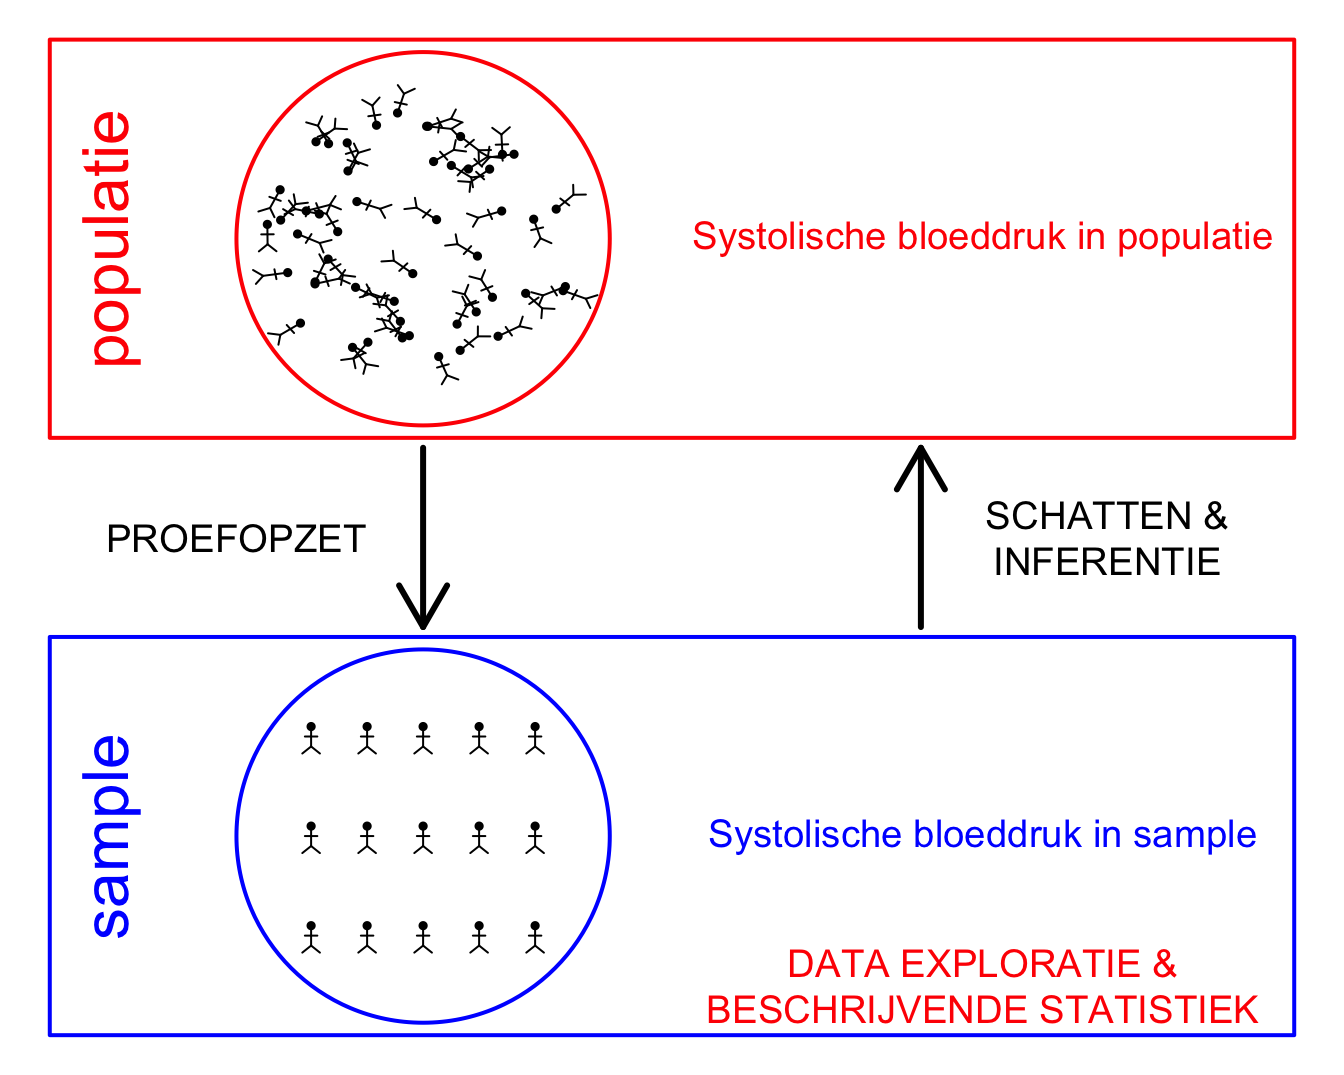
\includegraphics[width=1\linewidth]{Statistiek_2020_2021_files/figure-latex/pop2Samp2PopDataExpl-1} 

}

\caption{Verschillende stappen in een studie. In dit hoofdstuk ligt de focus op de data-exploratie en beschrijvende statistiek}\label{fig:pop2Samp2PopDataExpl}
\end{figure}

Dit hoofdstuk zullen werken rond een centrale dataset: de NHANES studie.

\begin{example}[NHANES studie]
\begin{example}

\protect\hypertarget{exm:nhanesEx}{}{\label{exm:nhanesEx} \iffalse (NHANES studie) \fi{} }

\end{example}
\end{example}

De National Health and Nutrition Examination Survey
(NHANES) wordt sinds 1960 op regelmatige basis of genomen. In dit voorbeeld maken we gebruik van de gegevens die werden verzameld tussen 2009-2012 bij 10000 Amerikanen en die werden opgenomen in het R-pakket NHANES. Er werd een groot aantal fysische, demografische, nutritionele, levelsstijl en gezondheidskarakteristieken gecollecteerd in deze studie (zie Tabel \ref{tab:nhanesDatExpl}). Merk op dat ontbrekende waarnemingen hier gecodeerd worden a.d.h.b. de code \texttt{NA} (Not Available / Missing Value)

\textbf{Einde voorbeeld}

\begin{table}[t]

\caption{\label{tab:nhanesDatExpl}Overzicht van een aantal variabelen uit de NHANES studie.}
\centering
\begin{tabular}{rlrlrrrrrll}
\toprule
ID & Gender & Age & Race1 & Weight & Height & BMI & BPSysAve & TotChol & SmokeNow & Smoke100\\
\midrule
51624 & male & 34 & White & 87.4 & 164.7 & 32.22 & 113 & 3.49 & No & Yes\\
51625 & male & 4 & Other & 17.0 & 105.4 & 15.30 & NA & NA & NA & NA\\
51630 & female & 49 & White & 86.7 & 168.4 & 30.57 & 112 & 6.70 & Yes & Yes\\
51638 & male & 9 & White & 29.8 & 133.1 & 16.82 & 86 & 4.86 & NA & NA\\
51646 & male & 8 & White & 35.2 & 130.6 & 20.64 & 107 & 4.09 & NA & NA\\
\addlinespace
51647 & female & 45 & White & 75.7 & 166.7 & 27.24 & 118 & 5.82 & NA & No\\
\bottomrule
\end{tabular}
\end{table}

\hypertarget{sec:univar}{%
\section{Univariate beschrijving van de variabelen}\label{sec:univar}}

In de regel begint men met een \emph{univariate} inspectie: elke variabele
wordt apart onderzocht. Het is absoluut aan te raden om hierbij eerst alle
ruwe gegevens te bekijken door middel van grafieken (zie verder) alvorens
naar samenvattingsmaten (zoals het gemiddelde) over te stappen. Dit laat toe
om een idee te krijgen hoe de geobserveerde waarden van een veranderlijke
verdeeld zijn in de studiegroep (bvb. welke verdeling de bloeddrukmetingen in de studie hebben)
en of er eventuele \emph{uitschieters} (d.i. extreme
metingen of \emph{outliers}) zijn. Met outliers worden observaties
aangegeven die ten opzichte van de geobserveerde verdeling van de waarden in
de data set, extreem zijn, buitenbeentjes.

\begin{Shaded}
\begin{Highlighting}[]
\CommentTok{\# De data van de NHANES studie bevindt zich in het}
\CommentTok{\# R package NHANES}
\KeywordTok{library}\NormalTok{(NHANES)  }\CommentTok{\#laad NHANES package}

\CommentTok{\# NHANES is een data frame met de gegevens De rijen}
\CommentTok{\# bevatten informatie over elk subject De kolommen}
\CommentTok{\# de variabelen die werden geregistreerd vb}
\CommentTok{\# variabele Gender, BMI, ... Een variabele (kolom)}
\CommentTok{\# kan uit de dataframe worden gehaald door gebruik}
\CommentTok{\# van het $ teken en de naam van de variabele We}
\CommentTok{\# slaan de frequentietabel voor variable Gender op}
\CommentTok{\# in object \textquotesingle{}tab\textquotesingle{}}

\NormalTok{tab \textless{}{-}}\StringTok{ }\KeywordTok{table}\NormalTok{(NHANES}\OperatorTok{$}\NormalTok{Gender)}
\NormalTok{tab}
\end{Highlighting}
\end{Shaded}

\begin{verbatim}
## 
## female   male 
##   5020   4980
\end{verbatim}

We maken nu een barplot voor de variabele gender

\begin{enumerate}
\def\labelenumi{\arabic{enumi}.}
\tightlist
\item
  We pipen de NHANES data naar ggplot
\item
  Als aestetics definiëren we x=Gender
\item
  We voegen een laag met een barplot toe via de functie \texttt{geom\_bar}. We definiëren de kleur via het argument \texttt{fill}
\end{enumerate}

\begin{Shaded}
\begin{Highlighting}[]
\NormalTok{NHANES }\OperatorTok{\%\textgreater{}\%}\StringTok{ }\KeywordTok{ggplot}\NormalTok{(}\KeywordTok{aes}\NormalTok{(}\DataTypeTok{x =}\NormalTok{ Gender)) }\OperatorTok{+}\StringTok{ }\KeywordTok{geom\_bar}\NormalTok{(}\DataTypeTok{fill =} \StringTok{"steelblue"}\NormalTok{)}
\end{Highlighting}
\end{Shaded}

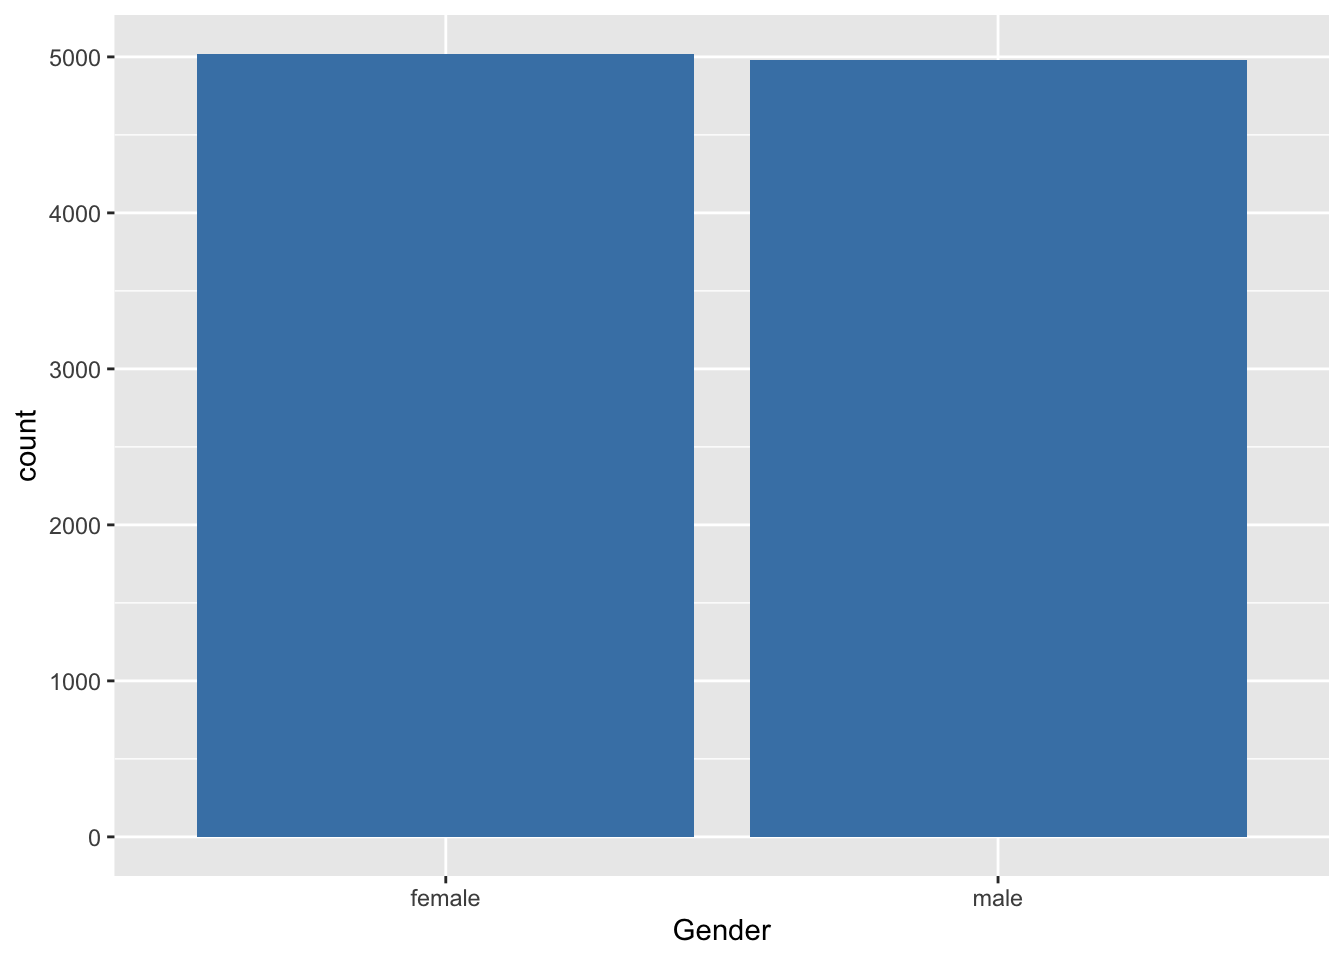
\includegraphics{Statistiek_2020_2021_files/figure-latex/unnamed-chunk-88-1.pdf}
Er zijn weinig methoden voorhanden om \emph{nominale} variabelen te
beschrijven. In Voorbeeld \ref{exm:nhanesEx} is de variable \emph{Gender}
kwalitatief nominaal.
Alles is gezegd over de verdeling van het geslacht als we weergeven hoeveel vrouwen en mannen zijn opgenomen in de studie.

We stellen vast dat 5020 van de 10000 subjecten, ofwel 50.2\% vrouwen in de studie zijn opgenomen.

Een staafdiagram geeft op de X-as de mogelijke uitkomsten van de variabele
aan (bvb. geslacht). Daarbovenop komt een staaf met hoogte evenredig aan
het totaal aantal keer dat die waarde voorkomt in de dataset. De staven staan los van elkaar met een breedte die constant is, maar verder willekeurig. Als de steekproef
representatief is voor de populatie, dan
krijgen we hier misschien een eerste impressie dat er iets meer vrouwen zijn in de populatie.

Voor \emph{numerieke continue variabelen} wordt het moeilijk om de
frequentie van alle uitkomstwaarden in een tabel te klasseren omdat veel
waarden hoogstens 1 keer voorkomen. Het \emph{tak-en-blad diagram} (in het
Engels: \emph{stem and leaf plot} is een middel om toch nog alle
uitkomsten weer te geven. Een voorbeeld is weergegeven in onderstaande R-output voor het BMI in de NHANES studie.

\begin{Shaded}
\begin{Highlighting}[]
\KeywordTok{stem}\NormalTok{(NHANES}\OperatorTok{$}\NormalTok{BMI)}
\end{Highlighting}
\end{Shaded}

\begin{verbatim}
## 
##   The decimal point is 1 digit(s) to the right of the |
## 
##   1 | 33333333333333333344444444444444444444444444444444444444444444444444+37
##   1 | 55555555555555555555555555555555555555555555555555555555555555555555+1389
##   2 | 00000000000000000000000000000000000000000000000000000000000000000000+2264
##   2 | 55555555555555555555555555555555555555555555555555555555555555555555+2610
##   3 | 00000000000000000000000000000000000000000000000000000000000000000000+1693
##   3 | 55555555555555555555555555555555555555555555555555555555555555555555+635
##   4 | 00000000000000000000000000000000000000000000000000000000000000000000+255
##   4 | 55555555555555555555555556666666666666666666666666666666666777777777+46
##   5 | 0000011111122222233333444444444444
##   5 | 5556677777789999
##   6 | 133444
##   6 | 567899
##   7 | 
##   7 | 
##   8 | 111
\end{verbatim}

Hier wordt van alle uitkomsten het eerste cijfer of de eerste paar cijfers
op een verticale lijn in volgorde uitgezet in de vorm van een boomstam.
Daaraan worden horizontaal de bladeren gehecht, met name de laatste cijfers
van de geobserveerde uitkomsten. De output geeft bijvoorbeeld aan dat er 3 personen zijn waarvan het afgeronde BMI 55 bedraagt, 2 personen met een afgerond BMI van 56, \ldots.
Gezien de studie zo groot is, is het tak-en-blad diagram niet erg praktisch voor dit voorbeeld.

In een tak-en-blad diagram krijgt men alle individuele uitkomsten nagenoeg
exact te zien, terwijl de vorm die het diagram aanneemt reeds een idee van
de verdeling geeft zoals in een histogram (zie verder). Een vuistregel om de
vorm van de verdeling het best te zien is het aantal takken ongeveer gelijk
te maken aan \(1 + \sqrt{n}\), waarbij \(n\) het aantal observaties voorstelt.
Dit aantal kan uiteraard aangepast worden aan de omstandigheden.
Een populair alternatief voor het tak en blad diagram is de \emph{eenvoudige frequentietabel}. Deze kan men bekomen door de continue variabele (bvb. BMI) om te zetten in een kwalitatieve ordinale variabele, waarvoor vervolgens een frequentietabel wordt weergegeven.

Het grafisch equivalent van dergelijke frequentietabel noemt een \emph{histogram}, hetgeen men in \texttt{ggplot} bekomt via

\begin{enumerate}
\def\labelenumi{\arabic{enumi}.}
\tightlist
\item
  Pipe de data van de NHANES study naar de \texttt{ggplot} functie
\item
  Selecteer de variable BMI als de data om in de x-coordinaat te visualiseren voor het aestetics argument van ggplot gebruik hiervoor de \texttt{aes} functie
\item
  Voeg een laag toe voor het histogram. Wanneer je geen aestetics \texttt{aes} meegeeft verkrijg je standaard absolute frequenties. Met \texttt{fill=..counts..} in de aestetics kan je de balken van het histogram inkleuren a.d.h.v. de absolute frequenties.
\item
  Indien je het wenst kan je op een histogram met densities ook nog een laag toevoegen met een niet parametrische densiteitsschatter voor de verdeling d.m.v. de \texttt{geom\_density} functie.
\end{enumerate}

\begin{Shaded}
\begin{Highlighting}[]
\NormalTok{NHANES }\OperatorTok{\%\textgreater{}\%}\StringTok{ }\KeywordTok{ggplot}\NormalTok{(}\KeywordTok{aes}\NormalTok{(}\DataTypeTok{x =}\NormalTok{ BMI)) }\OperatorTok{+}\StringTok{ }\KeywordTok{geom\_histogram}\NormalTok{(}\KeywordTok{aes}\NormalTok{(}\DataTypeTok{y =}\NormalTok{ ..density.., }
    \DataTypeTok{fill =}\NormalTok{ ..count..), }\DataTypeTok{bins =} \DecValTok{30}\NormalTok{) }\OperatorTok{+}\StringTok{ }\KeywordTok{geom\_density}\NormalTok{()}
\end{Highlighting}
\end{Shaded}

\begin{figure}

{\centering 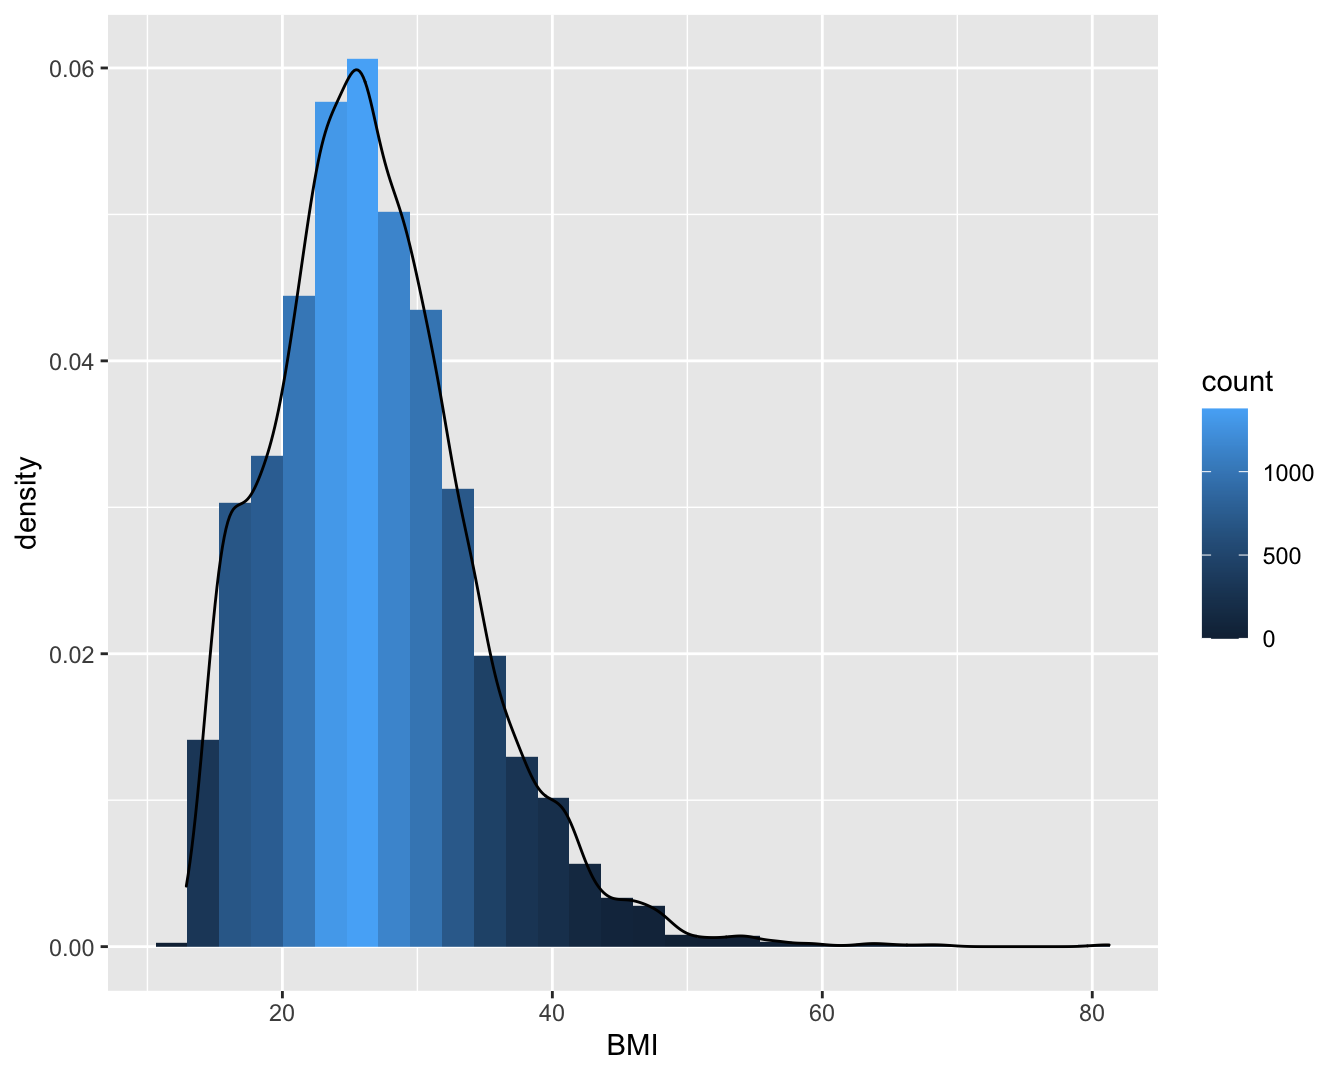
\includegraphics[width=1\linewidth]{Statistiek_2020_2021_files/figure-latex/histo-1} 

}

\caption{Histogram van het BMI in de NHANES studie.}\label{fig:histo}
\end{figure}

Wanneer alle klassen
een zelfde breedte hebben, worden de absolute of relatieve frequenties per
klasse weergegeven door de hoogte van de bijhorende kolom. Bij ongelijke
klassebreedtes is het de oppervlakte van de kolom die met de bijhorende
klassefrequentie correspondeert. Omdat een histogram met ongelijke
klassebreedtes moeilijker te interpreteren is, zijn histogrammen met gelijke
klassebreedtes vaak te verkiezen. Als histogrammen voor verschillende
groepen bekeken worden, vergemakkelijkt het gebruik van \emph{relatieve}
frequenties i.p.v. absolute frequenties de visuele vergelijkbaarheid.

Op het histogram in Figuur \ref{fig:histo} worden densiteiten
weergegeven en klassen met een breedte iets meer dan 5 eenheden.

De keuze van het aantal klassen is van belang bij een histogram. Als er te
weinig klassen zijn, dan gaat veel informatie verloren. Als er teveel zijn,
dan wordt het algemene patroon verdoezeld door een grote hoeveelheid overbodige
details. Gewoonlijk kiest men tussen 5 en 15 intervallen, maar de specifieke
keuze hangt af van het beeld van het histogram dat men te zien krijgt.

Een histogram is vooral geschikt om de distributie te schatten in grote datasets. Daar kan men dan veel intervallen gebruiken. Daarom heeft de ggplot functie standaard 30 intervallen.

Indien een voldoende aantal gegevens beschikbaar is, dan kan men een
gladdere indruk van de verdeling van de gegevens bekomen door een zogenaamde \emph{kernel density schatter} te bepalen. Zo'n schatter is een positieve functie die genormaliseerd is in die zin dat de oppervlakte onder de functie 1 is. Ze kan zo geïnterpreteerd worden dat de oppervlakte onder de functie tussen 2 punten \(a\) en \(b\) op de X-as, de kans voorstelt dat een lukrake meting in het interval \([a,b]\) gevonden wordt. Figuur \ref{fig:histo} toont een histogram met kernel density schatter van de het BMI.

De verdeling kan ook geëvalueerd worden aan de hand van een \emph{box-and-whisker-plot}, kortweg \emph{boxplot} genoemd. Deze is
meer compact dan een histogram en laat om die reden gemakkelijker
vergelijkingen tussen verschillende groepen toe (zie verder). Een Boxplot voor het BMI wordt getoond in Figuur \ref{fig:boxBMI}. De boxplot toont een
doos lopend van het 25\% tot 75\% percentiel met een lijntje ter hoogte van de
mediaan (het 50\% percentiel) en verder 2 snorharen. Die laatste kunnen in principe lopen tot het
minimum en maximum, of tot het 2.5\% en 97.5 \% of 5\% en 95\% percentiel.
R kiest voor de kleinste en de grootste geobserveerde waarde die geen
outlier of extreme waarde zijn. Een meting wordt hierbij een outlier genoemd
wanneer ze meer dan 1.5 keer de boxlengte beneden het eerste of boven het
derde kwartiel ligt. Een meting wordt een extreme waarde genoemd wanneer ze
meer dan 3 keer de boxlengte beneden het eerste of boven het derde kwartiel
ligt.

\begin{definition}[percentiel]
\begin{definition}

\protect\hypertarget{def:unnamed-chunk-90}{}{\label{def:unnamed-chunk-90} \iffalse (percentiel) \fi{} }

\end{definition}
\end{definition}

Het \emph{25\% percentiel} of \emph{25\% kwantiel} \(x_{25}\) van een
reeks waarnemingen wordt gedefinieerd als een uitkomstwaarde \(x_{25}\) zodat
minstens \(25\%\) van die waarnemingen kleiner of gelijk zijn aan \(x_{25}\) en
minstens \(75\%\) van die waarnemingen groter of gelijk zijn aan \(x_{25}\). Het
\emph{75\% percentiel} of \emph{75\% kwantiel} van een reeks
waarnemingen definieert men als een uitkomstwaarde \(x_{75}\) zodat minstens 75\%
kleiner of gelijk zijn aan \(x_{75}\) en minstens \(25\%\) van die waarnemingen
groter of gelijk zijn aan \(x_{75}\). Algemeen wordt het \emph{\(k\%\)
percentiel} van een reeks waarnemingen gedefinieerd als een waarde (van \(x\))
waarvoor de cumulatieve frequentie gelijk is aan \(k/100.\) Als er meerdere
observaties aan voldoen neemt men vaak het gemiddelde van die waarden.

\textbf{Einde definitie}

In R kunnen die als volgt worden bekomen

\begin{Shaded}
\begin{Highlighting}[]
\KeywordTok{quantile}\NormalTok{(NHANES}\OperatorTok{$}\NormalTok{BMI, }\KeywordTok{c}\NormalTok{(}\FloatTok{0.25}\NormalTok{, }\FloatTok{0.5}\NormalTok{, }\FloatTok{0.75}\NormalTok{), }\DataTypeTok{na.rm =} \OtherTok{TRUE}\NormalTok{)}
\end{Highlighting}
\end{Shaded}

\begin{verbatim}
##   25%   50%   75% 
## 21.58 25.98 30.89
\end{verbatim}

\begin{figure}

{\centering 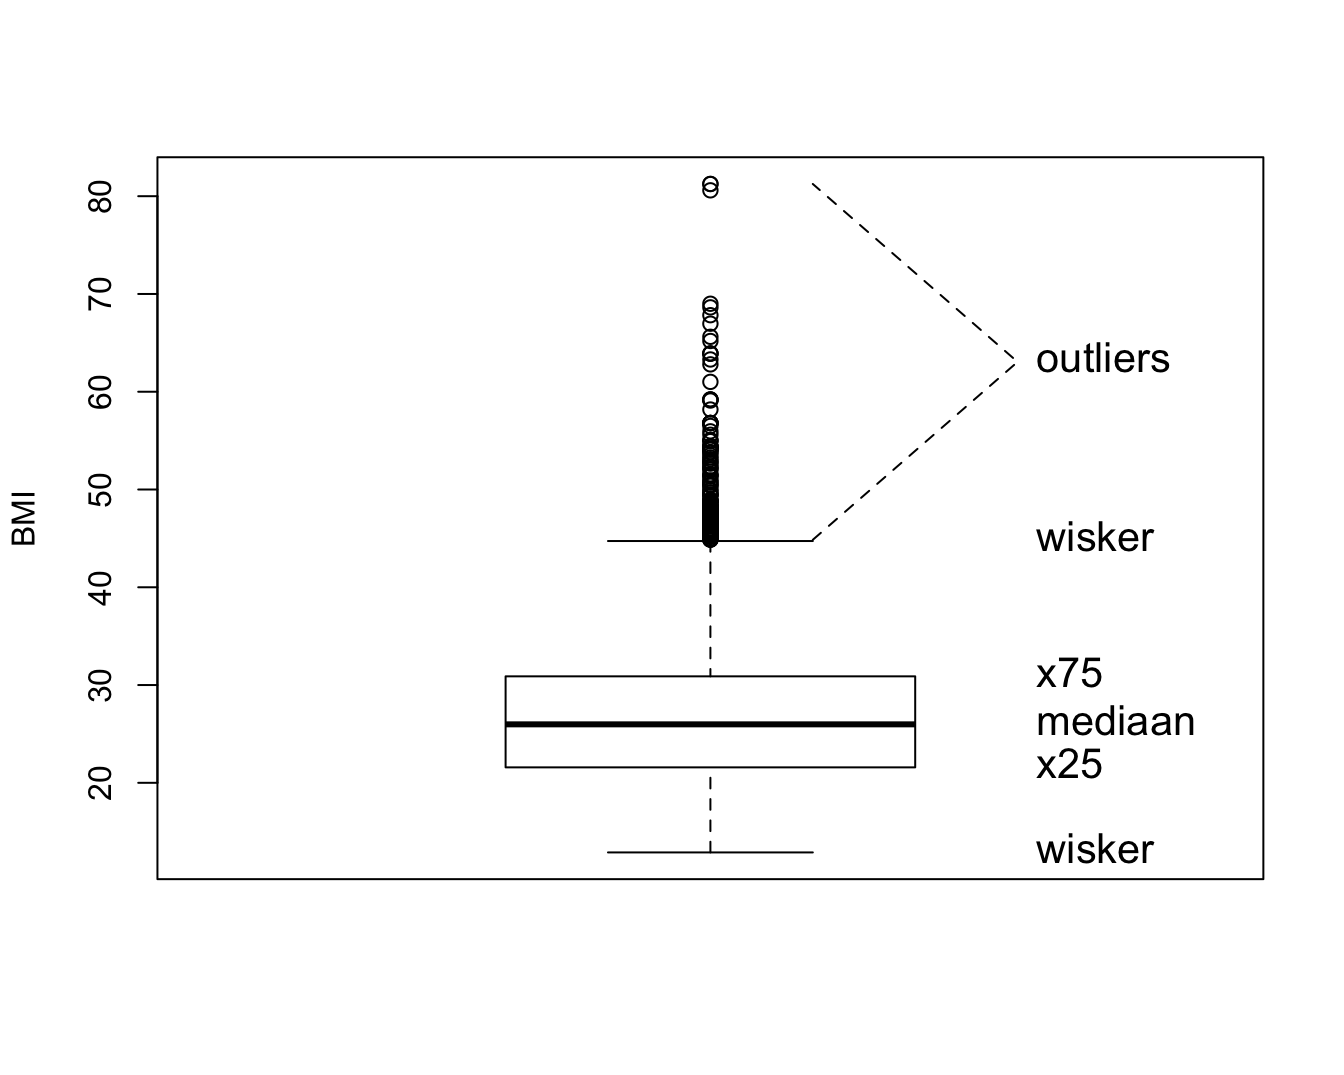
\includegraphics[width=1\linewidth]{Statistiek_2020_2021_files/figure-latex/boxBMI-1} 

}

\caption{Boxplot van BMI in de NHANES studie.}\label{fig:boxBMI}
\end{figure}

In ggplot maak je de boxplot als volgt:

\begin{Shaded}
\begin{Highlighting}[]
\NormalTok{NHANES }\OperatorTok{\%\textgreater{}\%}\StringTok{ }\KeywordTok{ggplot}\NormalTok{(}\KeywordTok{aes}\NormalTok{(}\DataTypeTok{x =} \StringTok{""}\NormalTok{, }\DataTypeTok{y =}\NormalTok{ BMI)) }\OperatorTok{+}\StringTok{ }\KeywordTok{geom\_boxplot}\NormalTok{()}
\end{Highlighting}
\end{Shaded}

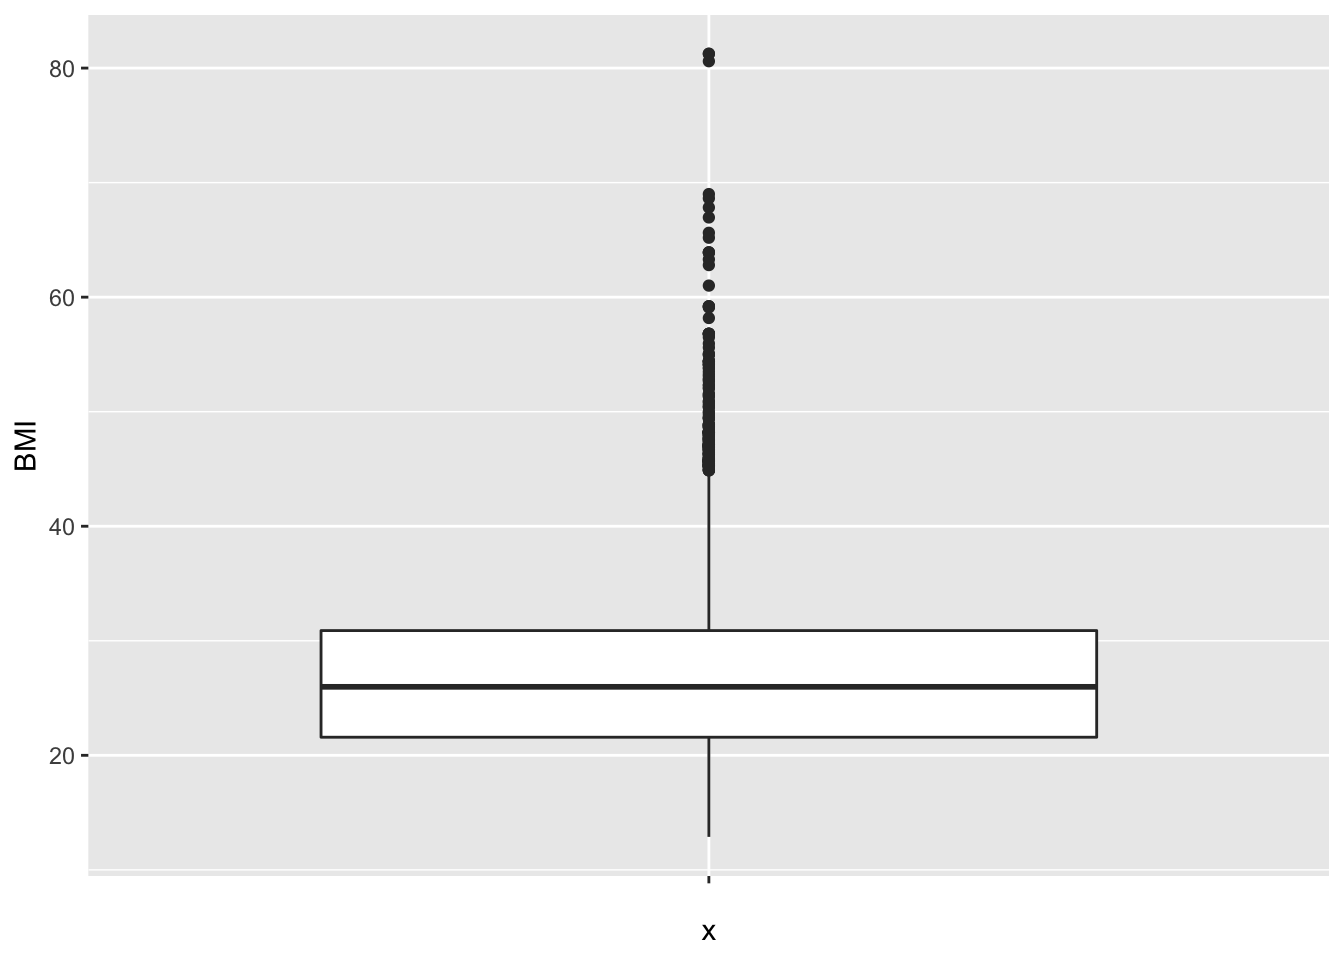
\includegraphics{Statistiek_2020_2021_files/figure-latex/unnamed-chunk-92-1.pdf}

Bij de inspectie van een dataset speelt het detecteren van outliers in het
algemeen een belangrijke rol. Ze kunnen wijzen op fouten, zoals tikfouten of
andere fouten die gecheckt en gecorrigeerd moeten worden. Als het geen
foutief genoteerde waarden zijn, dan kan het soms wijzen op een subject dat niet
echt in de studiepopulatie thuis hoort. Als het in
alle opzichten om een bona fide waarde gaat, dan nog is het belangrijk om
outliers te detecteren: ze kunnen zeer invloedrijk zijn op de schatting van
statistische parameters (zie Sectie \ref{sec:summarize}). Als de conclusies
van een studie anders liggen met of zonder inclusie van de outlier, dan is
dit een ongewenst fenomeen. Men wil immers nooit dat 1 observatie beslissend
is voor de conclusies. Dit soort onzekerheid ondermijnt de geloofwaardigheid
van de onderzoeksresultaten en vraagt om verdere studie. Binnen de
statistiek bestaat een grote waaier aan technieken, zogenaamde
\emph{robuuste statistische technieken}, die erop gericht zijn om de invloed van
outliers te minimaliseren. In deze cursus gaan we hier slechts in zeer
beperkte mate op in (zie Sectie \ref{sec:summarize}, mediaan).

\hypertarget{sec:summarize}{%
\section{Samenvattingsmaten voor continue variabelen}\label{sec:summarize}}

Een histogram levert reeds een sterke samenvatting van de geobserveerde,
continue gegevens, maar in wetenschappelijke rapporten is er zelden
plaats om per geobserveerde variabele dergelijke grafiek voor te stellen. Om
die reden is vaak een veel drastischere samenvattingsmaat noodzakelijk. In deze
sectie geven we aan hoe de centrale locatie van de gegevens kan beschreven
worden, alsook de spreiding van die gegevens rond hun centrale locatie.

\hypertarget{maten-voor-de-centrale-ligging}{%
\subsection{Maten voor de centrale ligging}\label{maten-voor-de-centrale-ligging}}

\begin{definition}[rekenkundig gemiddelde]
\begin{definition}

\protect\hypertarget{def:unnamed-chunk-93}{}{\label{def:unnamed-chunk-93} \iffalse (rekenkundig gemiddelde) \fi{} }

\end{definition}
\end{definition}

Het \textbf{(rekenkundig) gemiddelde} \(\overline{x}\) (spreek uit: \emph{x-streep}
of \emph{x-bar}) van een reeks waarnemingen \(x_i, i=1, 2, \dots, n\) is per
definitie de som van de observaties gedeeld door hun aantal \(n\):

\[\overline{x}= \frac{x_1 + x_2 + \dots + x_n}{n} =\sum_{i=1}^n x_i \frac{1}{n} \]

\textbf{Einde definitie}

Merk op dat het rekenkundig gemiddelde ook verkregen zou worden als gemiddelde voor een discrete distributie met kansen van 1/n op elke waarde uit de steekproef.
Wanneer we het steekproefgemiddelde gebruiken dan schatten we de distributie in de populatie als het ware aan de hand van de empirische distributie van de data. We maken dus geen distributionele veronderstellingen hiervoor.

Een groot voordeel van het gemiddelde als een maat voor de centrale locatie
van de observaties is dat het alle data-waarden efficiënt gebruikt vanuit
statistisch perspectief. Dit wil zeggen dat ze (onder bepaalde statistische modellen)
het maximum aan informatie
uit de gegevens haalt en om die reden relatief gezien zeer stabiel blijft
wanneer ze herberekend wordt op basis van een nieuwe, even grote steekproef
die onder identieke omstandigheden werd bekomen. Bovendien beschrijft het
gemiddelde ook verschillende belangrijke modellen voor de verdeling van de
gegevens, zoals de Normale verdeling (zie Sectie \ref{sec:normal}). Een
groot nadeel van het gemiddelde is dat het zeer gevoelig is aan de
aanwezigheid van outliers in de dataset. Om die reden is het vooral een
interessante maat van locatie wanneer de verdeling van de observaties (zoals
weergegeven door bijvoorbeeld een histogram) min of meer symmetrisch is.

\begin{Shaded}
\begin{Highlighting}[]
\KeywordTok{mean}\NormalTok{(NHANES}\OperatorTok{$}\NormalTok{BMI, }\DataTypeTok{na.rm =} \OtherTok{TRUE}\NormalTok{)}
\end{Highlighting}
\end{Shaded}

\begin{verbatim}
## [1] 26.66014
\end{verbatim}

\begin{Shaded}
\begin{Highlighting}[]
\CommentTok{\# opnieuw is de na.rm statement hier nodig omdat}
\CommentTok{\# ontbrekende waarden voorkomen.}
\end{Highlighting}
\end{Shaded}

\emph{Indien men de grootste observatie (81.25) vervangt door 8125 om als het ware ene tikfout voor te stellen, dan wijzigt het rekenkundig gemiddelde naar 27.5 en dat terwijl er bijna 10000 BMI metingen zijn. Merk op dat het gemiddelde vrij sterk beïnvloed kan worden door één outlier.}

\textbf{Eigenschap}

Als alle uitkomsten \(x_i\) met een willekeurige constante \(a\)
worden vermenigvuldigd, dan ook het gemiddelde van die reeks uitkomsten. Als
bij alle uitkomsten een constante \(a\) wordt opgeteld, dan ook bij het
gemiddelde van die reeks uitkomsten. Formeel betekent dit:

\begin{eqnarray*}
\overline{ax} &= &a \overline{x} \\
\overline{a + x} &= &a + \overline{x}
\end{eqnarray*}

Voor 2 reeksen getallen \(x_i\) en \(y_i\), \(i=1,...,n\), geldt dat het
gemiddelde van de som van de observaties gelijk is aan de som van hun
gemiddelden:

\begin{equation*}
\overline{x + y} = \overline{x} + \overline{y}.
\end{equation*}

Als de gegevens \(x_i\) enkel de waarden 0 of 1 aannemen, dan is \(\overline{x}\)
de proportie subjecten voor wie de waarde 1 werd geobserveerd. Immers, zij \(n_1\) het aantal subjecten binnen de groep van \(n\) subjecten waarvoor de
waarde 1 werd geobserveerd, dan is

\begin{equation*}
\overline{x}= \sum_{i=1}^n \frac{x_i}{n} = \frac{n_1}{n}.
\end{equation*}

Bijvoorbeeld, als we de variabele \textbf{Gender} zó
coderen dat mannen een waarde 0 aannemen en vrouwen een waarde 1, dan is het
gemiddelde van de variabele \textbf{Gender} gelijk aan 50.2\%, hetgeen de proportie is van het aantal vrouwen in de studie. Een percentage kan dus
steeds opgevat worden als het gemiddelde van een geschikte variabele.

\textbf{Einde eigenschap}

Een centrale maat die robuuster reageert dan het gemiddelde, d.w.z. minder
of niet gevoelig is aan outliers, is de \emph{mediaan} of het \emph{50\% percentiel}.

\begin{definition}[mediaan]
\begin{definition}

\protect\hypertarget{def:unnamed-chunk-95}{}{\label{def:unnamed-chunk-95} \iffalse (mediaan) \fi{} }

\end{definition}
\end{definition}

De \textbf{mediaan}, het \textbf{50\% percentiel} of het \textbf{50\%
kwantiel} \(x_{50}\) van een reeks waarnemingen \(x_i, i=1, 2, \dots, n\) is per
definitie een uitkomstwaarde \(x_{50}\) zodat minstens \(50\%\) van die
waarnemingen groter of gelijk zijn aan \(x_{50}\) en minstens \(50\%\) van die
waarnemingen kleiner of gelijk zijn aan \(x_{50}\).

\textbf{Einde definitie}

Om de mediaan te schatten, rangschikt men eerst de gegevens volgens grootte.
Als het aantal observaties \(n\) oneven is, dan is een schatting voor de
mediaan de middelste waarneming. Indien \(n\) even is, dan zijn er 2 middelste
waarnemingen en schat men de mediaan (meestal) als hun gemiddelde. Een
voordeel van de mediaan is dat ze niet gevoelig is aan outliers. In het bijzonder kan
ze vaak nuttig aangewend worden wanneer sommige gegevens \emph{gecensureerd}
zijn. Dit wil zeggen dat men voor een aantal gegevens enkel weet dat ze
boven of onder een bepaalde drempelwaarde liggen.

\begin{Shaded}
\begin{Highlighting}[]
\KeywordTok{median}\NormalTok{(NHANES}\OperatorTok{$}\NormalTok{BMI, }\DataTypeTok{na.rm =} \OtherTok{TRUE}\NormalTok{)}
\end{Highlighting}
\end{Shaded}

\begin{verbatim}
## [1] 25.98
\end{verbatim}

\begin{Shaded}
\begin{Highlighting}[]
\CommentTok{\# Merk op dat we hier gebruik maken van het}
\CommentTok{\# argument na.rm=TRUE Dit komt omdat we niet}
\CommentTok{\# beschikken over het BMI voor elke persoon:}
\CommentTok{\# ontbrekende waarnemingen Die worden in R als een}
\CommentTok{\# NA voorgesteld Als we het argument na.rm=TRUE}
\CommentTok{\# gebruiken wordt de mediaan berekend op basis van}
\CommentTok{\# de beschikbare observaties}
\end{Highlighting}
\end{Shaded}

Indien men de grootste observatie (81.25) vervangt 8125, dan wijzigt de mediaan niet.
Merk ook op dat de mediaan lager is dan het gemiddelde, hij is minder gevoelig voor de outliers in de dataset.

\begin{definition}[modus]
\begin{definition}

\protect\hypertarget{def:unnamed-chunk-97}{}{\label{def:unnamed-chunk-97} \iffalse (modus) \fi{} }

\end{definition}
\end{definition}

De \textbf{modus} van een reeks observaties is de waarde die het meest
frequent is, of wanneer de gegevens gegroepeerd worden, de klasse met de
hoogste frequentie.

\textbf{Einde definitie}

De modus wordt niet vaak gebruikt in statistische analyse omdat haar waarde
sterk afhangt van de nauwkeurigheid waarmee de gegevens werden gemeten. Zo
is de modus van de reeks observaties \(1, 1, 1, 1.5, 1.75, 1.9, 2, 2.1, 2.4\)
gelijk aan 1, maar wordt ze 2 wanneer alle observaties afgerond worden tot
gehele getallen. Bovendien is de modus niet eenvoudig te schatten voor
continue data waar de frequentie van elke geobserveerde waarde meestal 1 is.
De modus is daarom het meest zinvol voor kwalitatieve en discrete numerieke
gegevens, waar ze de meest frequente klasse aanduidt.

Als de observaties uit een \emph{symmetrische verdeling} afkomstig zijn,
vallen de mediaan en het gemiddelde nagenoeg samen (als de geobserveerde
verdeling perfect symmetrisch is, vallen ze theoretisch exact samen).
De beste schatter voor het centrum van de verdeling op basis van de beschikbare
steekproef is dan het gemiddelde eerder dan de mediaan van die observaties.
Inderdaad, als men telkens opnieuw een lukrake steekproef neemt uit de
gegeven studiepopulatie en voor elke steekproef het gemiddelde en de mediaan
berekent, dan zal het gemiddelde minder variëren van steekproef tot
steekproef dan de mediaan. Ze is bijgevolg stabieler en wordt daarom een
\emph{meer precieze schatter} genoemd. Intuïtief kan men begrijpen dat
het gemiddelde meer informatie uit de gegevens gebruikt: niet alleen of iets
groter of kleiner is dan \(x_{50}\) maar ook hoeveel groter of kleiner de
exacte waarde van elke observatie is, wordt in de berekening betrokken.

\begin{definition}[scheve verdeling]
\begin{definition}

\protect\hypertarget{def:unnamed-chunk-98}{}{\label{def:unnamed-chunk-98} \iffalse (scheve verdeling) \fi{} }

\end{definition}
\end{definition}

Een niet-symmetrische verdeling wordt \textbf{scheef} genoemd. Als de
waarden rechts van de mediaan verder uitlopen dan links, dan is de verdeling
\emph{scheef naar rechts} (in het Engels: \emph{positively skew}) en is
het gemiddelde (meestal) groter dan de mediaan. Als de waarden links van de
mediaan verder uitlopen dan rechts, dan is de verdeling \emph{scheef naar
links} (in het Engels: \emph{negatively skew}) en is het gemiddelde
(meestal) kleiner dan de mediaan.

\textbf{Einde definitie}

Voor een niet-symmetrische verdeling is de mediaan veelal een beter
interpreteerbare maat dan het gemiddelde omdat ze minder beïnvloed is
door de staarten van de verdeling en daarom beter het centrum van de
verdeling aanduidt. Maar in sommige gevallen, zoals bijvoorbeeld voor `de
gemiddelde opbrengst per week', blijft het gemiddelde zinvol omdat het
meteen verwijst naar de totale opbrengst over alle weken (gelijk aan \(n\)
keer het gemiddelde als \(n\) weken werden geobserveerd). Ook voor
kwalitatieve variabelen kan een gemiddelde zinvol zijn. Voor binaire
nominale variabelen die als 1 of 0 gecodeerd zijn, geeft het gemiddelde
immers het percentage observaties gelijk aan 1 weer. Voor ordinale
variabelen die bijvoorbeeld gecodeerd zijn als \(1, 2, 3, ...\) levert het
gemiddelde soms nuttigere informatie dan de mediaan. Niettemin berust het
dan op de impliciete onderstelling dat een wijziging van score van 1 naar 2
even belangrijk is als een wijziging van 2 naar 3.

Om scheve verdelingen in een paar woorden te beschrijven is het vaak nuttig
om

\begin{itemize}
\tightlist
\item
  ofwel de gegevens te beschrijven in termen van percentielen,
\item
  ofwel de gegevens te transformeren naar een andere schaal (bvb. door
  logaritmen te nemen), zodat ze op de nieuwe schaal bij benadering
  symmetrisch verdeeld zijn.
\end{itemize}

Wanneer het gemiddelde groter is dan de mediaan en alle metingen positief zijn (vb concentraties, BMI), dan is een logaritmische
transformatie van de gegevens vaak nuttig om de scheefheid weg te nemen. In
dit geval is vooral het \emph{geometrisch gemiddelde} interessant.

\begin{definition}[geometrisch gemiddelde]
\begin{definition}

\protect\hypertarget{def:unnamed-chunk-99}{}{\label{def:unnamed-chunk-99} \iffalse (geometrisch gemiddelde) \fi{} }

\end{definition}
\end{definition}

Het \textbf{geometrische gemiddelde} van een reeks waarnemingen \(x_i, i=1, 2, \dots, n\) ontstaat door er de natuurlijke logaritme van te berekenen, het
gemiddelde hiervan te nemen en dit vervolgens terug te transformeren naar de
originele schaal door er de exponentiële functie van te nemen:

\begin{equation*}
\sqrt[n]{\prod\limits_{i=1}^n x_i} = \exp\left\{\frac{1}{n} \sum_{i=1}^n \log(x_i)\right\}
\end{equation*}

\textbf{Einde definitie}

\begin{itemize}
\item
  Geometrisch gemiddelde ligt dichter bij de mediaan dan het gemiddelde
\item
  log-transformatie verwijdert scheefheid
\item
  Is vaak een meer geschikte maat voor centrale locatie dan de mediaan:
\end{itemize}

\begin{enumerate}
\def\labelenumi{\arabic{enumi}.}
\tightlist
\item
  Gebruikt alle observatie: is meer precies
\item
  Is het rekenkundig gemiddelde van log-transformeerde data \(\rightarrow\) klassieke statistische methoden kunnen direct worden gebruikt, b.v. hypothese testen en betrouwbaarheidsintervallen (zie hoofdstuk 5)
\item
  Veel biologische en chemische variabelen zoals concentraties, intensiteiten, etc kunnen niet negatief zijn.
\item
  Verschillen op log schaal hebben de betekenis van een \texttt{log\ fold\ change}:
\end{enumerate}

\[
\log (B) - \log(A)= \log(\frac{B}{A})=\log(FC_\text{B vs A})
\]

\begin{itemize}
\item
  In Genomics wordt de \(\log_2\) transformatie veel gebruikt.
\item
  Een verschil van 1 op \(\log_2\) schaal betekent een verdubbeling op de originele schaal \(FC=2\).
\end{itemize}

\begin{Shaded}
\begin{Highlighting}[]
\NormalTok{logSummary \textless{}{-}}\StringTok{ }\NormalTok{NHANES }\OperatorTok{\%\textgreater{}\%}\StringTok{ }\KeywordTok{filter}\NormalTok{(Gender }\OperatorTok{==}\StringTok{ "female"}\NormalTok{) }\OperatorTok{\%\textgreater{}\%}\StringTok{ }
\StringTok{    }\KeywordTok{summarize}\NormalTok{(}\DataTypeTok{logMean =} \KeywordTok{mean}\NormalTok{(BMI }\OperatorTok{\%\textgreater{}\%}\StringTok{ }\NormalTok{log2, }\DataTypeTok{na.rm =} \OtherTok{TRUE}\NormalTok{), }
        \DataTypeTok{sd =} \KeywordTok{sd}\NormalTok{(BMI }\OperatorTok{\%\textgreater{}\%}\StringTok{ }\NormalTok{log2, }\DataTypeTok{na.rm =} \OtherTok{TRUE}\NormalTok{), }\DataTypeTok{mean =} \KeywordTok{mean}\NormalTok{(BMI, }
            \DataTypeTok{na.rm =} \OtherTok{TRUE}\NormalTok{), }\DataTypeTok{median =} \KeywordTok{median}\NormalTok{(BMI, }\DataTypeTok{na.rm =} \OtherTok{TRUE}\NormalTok{)) }\OperatorTok{\%\textgreater{}\%}\StringTok{ }
\StringTok{    }\KeywordTok{mutate}\NormalTok{(}\DataTypeTok{geoMean =} \DecValTok{2}\OperatorTok{\^{}}\NormalTok{logMean)}

\NormalTok{NHANES }\OperatorTok{\%\textgreater{}\%}\StringTok{ }\KeywordTok{filter}\NormalTok{(Gender }\OperatorTok{==}\StringTok{ "female"}\NormalTok{) }\OperatorTok{\%\textgreater{}\%}\StringTok{ }\KeywordTok{ggplot}\NormalTok{(}\KeywordTok{aes}\NormalTok{(}\DataTypeTok{x =}\NormalTok{ BMI }\OperatorTok{\%\textgreater{}\%}\StringTok{ }
\StringTok{    }\NormalTok{log2)) }\OperatorTok{+}\StringTok{ }\KeywordTok{geom\_histogram}\NormalTok{(}\KeywordTok{aes}\NormalTok{(}\DataTypeTok{y =}\NormalTok{ ..density.., }\DataTypeTok{fill =}\NormalTok{ ..count..), }
    \DataTypeTok{bins =} \DecValTok{30}\NormalTok{) }\OperatorTok{+}\StringTok{ }\KeywordTok{geom\_density}\NormalTok{() }\OperatorTok{+}\StringTok{ }\KeywordTok{stat\_function}\NormalTok{(}\DataTypeTok{fun =}\NormalTok{ dnorm, }
    \DataTypeTok{color =} \StringTok{"red"}\NormalTok{, }\DataTypeTok{args =} \KeywordTok{list}\NormalTok{(}\DataTypeTok{mean =}\NormalTok{ logSummary}\OperatorTok{$}\NormalTok{logMean, }
        \DataTypeTok{sd =}\NormalTok{ logSummary}\OperatorTok{$}\NormalTok{sd))}
\end{Highlighting}
\end{Shaded}

\begin{figure}

{\centering 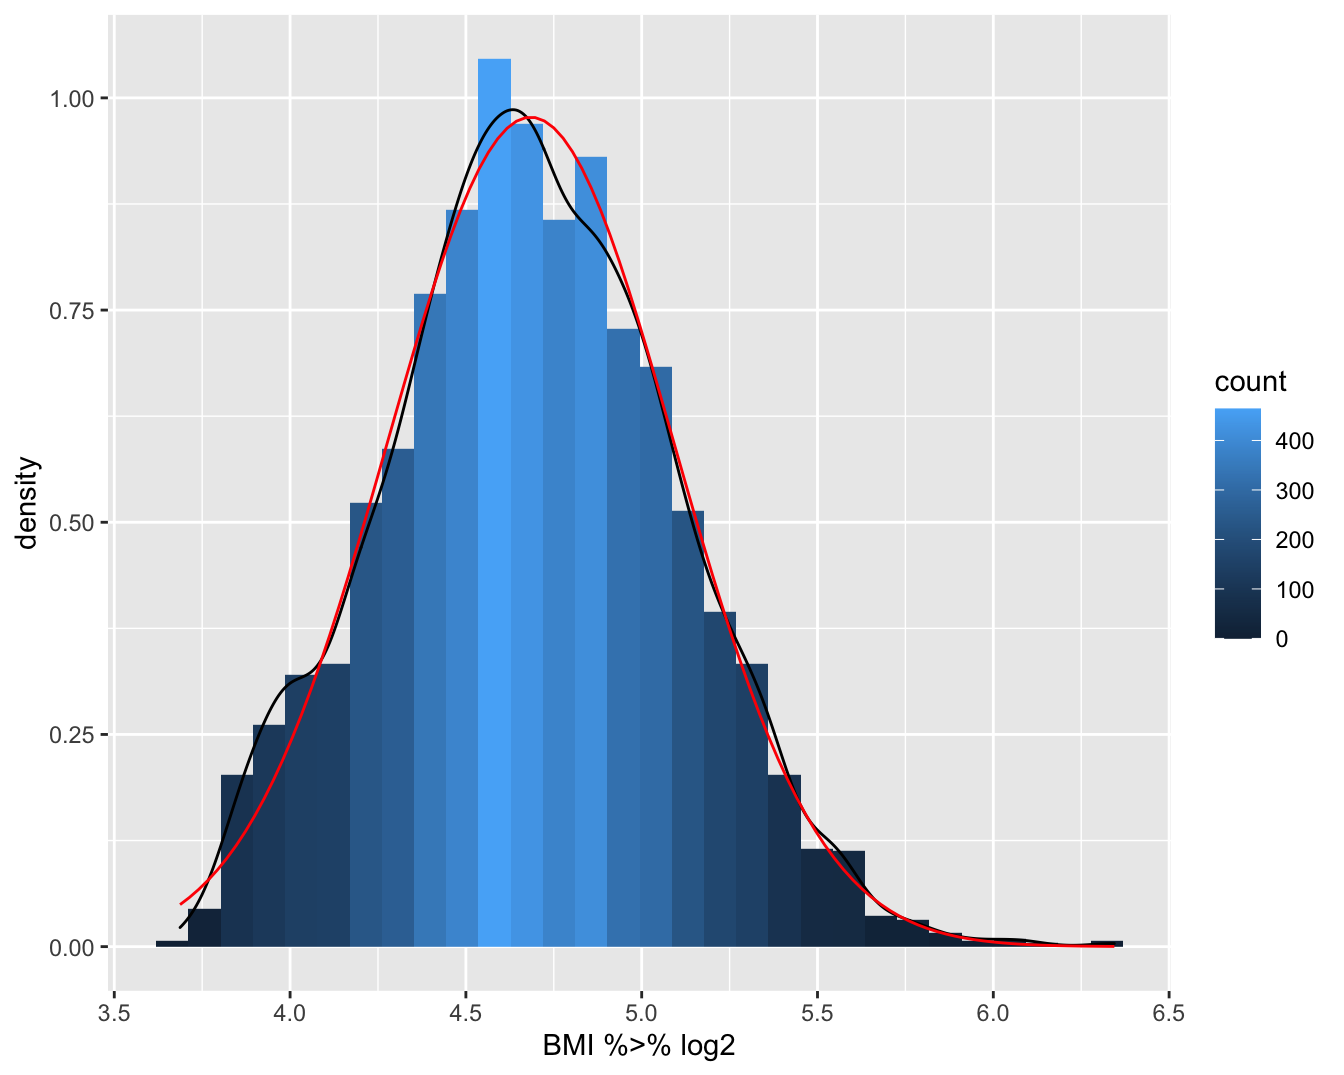
\includegraphics[width=1\linewidth]{Statistiek_2020_2021_files/figure-latex/histLogBMI-1} 

}

\caption{Boxplot van BMI en log(BMI) in de NHANES studie.}\label{fig:histLogBMI}
\end{figure}

\begin{Shaded}
\begin{Highlighting}[]
\NormalTok{logSummary}
\end{Highlighting}
\end{Shaded}

\begin{verbatim}
## # A tibble: 1 x 5
##   logMean    sd  mean median geoMean
##     <dbl> <dbl> <dbl>  <dbl>   <dbl>
## 1    4.68 0.408  26.8   25.6    25.7
\end{verbatim}

In situaties waar de log-transformatie inderdaad de scheefheid wegneemt, zal
het geometrisch gemiddelde dichter bij de mediaan liggen dan het gemiddelde.
Wanneer de verdeling scheef is, is ze soms zelfs een nuttigere maat voor centrale
locatie dan de mediaan:

\begin{enumerate}
\def\labelenumi{\arabic{enumi}.}
\item
  omdat ze ook gebruik maakt van de exacte waarden van de observaties en
  daarom doorgaans preciezer is dan de mediaan;
\item
  omdat ze, op een transformatie na, berekend wordt als een rekenkundig
  gemiddelde (weliswaar van de logaritmisch getransformeerde observaties) en
  algemene statistische technieken voor een gemiddelde (zoals
  betrouwbaarheidsintervallen (zie volgende hoofdstukken) en toetsen van hypothesen (zie volgende hoofdstukken) daardoor vrijwel rechtstreeks
  toepasbaar zijn voor geometrische gemiddelden.
\end{enumerate}

\begin{example}[BMI]
\begin{example}

\protect\hypertarget{exm:unnamed-chunk-100}{}{\label{exm:unnamed-chunk-100} \iffalse (BMI) \fi{} }

\end{example}
\end{example}

Het gemiddelde en mediane BMI bedraagt 26.66 en 25.98 , respectievelijk. Het gemiddelde is hier groter dan de mediaan omdat de BMI scheef verdeeld is naar rechts (zie Figuur \ref{fig:histLogBMI}). De verdeling wordt meer symmetrisch na log-transformatie. Het gemiddelde en mediane log-BMI liggen ook dichter bij elkaar en bedragen respectievelijk 3.25 en 3.26. De geometrisch gemiddelde BMI-concentratie bekomen we door de exponentiële functie te evalueren in 3.25, hetgeen ons 25.69 oplevert. Merk op dat dit inderdaad beter met de mediaan overeenstemt dan het rekenkundig gemiddelde.

\textbf{Einde voorbeeld}

Tot slot, vooraleer een eenvoudige maat voor de centrale ligging (en
spreiding) te construeren of interpreteren, is het goed om altijd eerst de
volledige verdeling te bekijken! Immers, stel dat men het gemiddelde of
mediaan berekent van gegevens uit een bimodale verdeling (d.i. een verdeling
met 2 modi, voor bvb. zieken en niet-zieke dieren). Dan kan het gemiddelde of
mediaan makkelijk een zeer zeldzame waarde aannemen die geenszins in de
buurt van 1 van beide maxima ligt.

\hypertarget{subsec:spreiding}{%
\subsection{Spreidingsmaten}\label{subsec:spreiding}}

Nadat de centrale ligging van de gegevens werd bepaald, is men in tweede
instantie geïnteresseerd in de spreiding van de gegevens rond
die centrale waarde. Er zijn verschillende redenen waarom daar interesse in bestaat:

\begin{enumerate}
\def\labelenumi{\arabic{enumi}.}
\tightlist
\item
  Om risico's te berekenen (zie Sectie \ref{sec:normal}) volstaat het niet om de centrale locatie van de gegevens te kennen, maar moet men bovendien weten hoeveel de gegevens rond die waarde variëren. Inderdaad, stel dat men wenst te weten welk percentage van de subjecten een BMI heeft van boven de 35. Wetende dat een geometrisch gemiddelde van 25.69 wordt geobserveerd, zal dat percentage relatief hoog zijn wanneer de metingen zeer gespreid zijn en relatief laag anders.
\item
  Veldbiologen zijn vaak geïnteresseerd in de mate waarin dieren of planten verspreid zijn over een zeker studiegebied. Op die manier kunnen ze immers leren over de relaties tussen individuen onderling en met hun omgeving. Daartoe zal men in de praktijk op verschillende plaatsen in het studiegebied tellingen maken van het aantal individuen op die plaats. Men kan aantonen dat, onder bepaalde veronderstellingen, individuen lukraak verspreid zijn over het studiegebied wanneer de spreiding op die tellingen, zoals gemeten door de variantie (zie verder), van dezelfde grootte-orde is als de gemiddelde telling. Indien de spreiding groter is, dan hebben individuen de neiging om zich te groeperen. Andersom, indien de spreiding op die tellingen lager is dan de gemiddelde telling, dan zijn de individuen zeer uniform verdeeld over het studiegebied.
\item
  Stel dat men een zekere uitkomst (bvb. het aantal species ongewervelde dieren in een stuk bodemkorst) wenst te vergelijken tussen 2 groepen (bvb. gebieden met en zonder bosbrand), dan zal men een duidelijk beeld van het groepseffect krijgen wanneer de uitkomst weinig gespreid is, maar een veel minder duidelijk beeld wanneer de gegevens meer chaotisch (en dus meer gespreid) zijn. Om uit te maken of een interventie-effect toevallig of systematisch is, moet men daarom een idee hebben van de spreiding op de gegevens.
\end{enumerate}

Dat uitkomsten variëren tussen individuen en binnen individuen omwille van
allerlei redenen ligt aan de basis van de statistische analyse van veel
fenomenen. Het goed beschrijven van variatie naast de centrale locatie van
de gegevens is daarom belangrijk! Hierbij zal men typisch een
onderscheid maken tussen variatie die men kan verklaren (door middel van
karakteristieken, zoals bijvoorbeeld de leeftijd, van de bestudeerde individuen) en onverklaarde variatie. We gaan
dieper in op dit onderscheid in Hoofdstuk \ref{chap:linReg} rond lineaire regressie.

Variatie betekent dat niet alle observaties \(x_i\) gelijk zijn aan het
gemiddelde \(\overline{x}\). De afwijking \(x_i - \bar{x}\) is om die reden
interessant. Het gemiddelde van die afwijkingen is echter altijd 0
(verifieer!) omdat positieve en negatieve afwijkingen mekaar opheffen.
Bijgevolg levert de gemiddelde afwijking geen goede maat op voor de variatie
en is het beter om bijvoorbeeld naar kwadratische afwijkingen \((x_i - \bar{x})^2\) te kijken. Het gemiddelde van die \emph{kwadratische afwijkingen rond het gemiddelde}, het gemiddelde dus van \((x_i - \bar{x})^2\), levert daarom
wel een goede maat op. Merk op dat we bij het berekenen van het gemiddelde niet delen door het aantal observaties \(n\), maar door \(n-1\) waarbij we corrigeren voor het feit dat we voor de berekening van de steekproef variantie 1 vrijheidsgraad hebben gespendeerd aan het schatten van het gemiddelde.

\begin{definition}[variantie]
\begin{definition}

\protect\hypertarget{def:unnamed-chunk-101}{}{\label{def:unnamed-chunk-101} \iffalse (variantie) \fi{} }

\end{definition}
\end{definition}

De \textbf{variantie} een reeks waarnemingen \(x_i, i=1, 2, \dots, n\) is per
definitie

\begin{equation*}
s^2_x = \sum_{i=1}^{n} \frac{(x_i - \bar{x})^2}{n-1}
\end{equation*}

Als duidelijk is om welke waarnemingen het gaat, wordt dit ook met \(s^2\)
genoteerd.

\textbf{Einde definitie}

Indien alle observaties gelijk waren en er dus geen variatie was, dan zou
hun variantie 0 bedragen. Hoe meer de gegevens uitgesmeerd zijn rond hun
gemiddelde, hoe groter \(s^2\). Helaas is de waarde van de variantie zelf niet
gemakkelijk te interpreteren. Dit is deels omdat door het kwadrateren de
variantie niet langer de dimensie van de oorspronkelijke waarnemingen heeft.
Handiger om mee te werken is daarom de \emph{standaarddeviatie} of \emph{
standaardafwijking}:

\begin{equation*}
s_x= \sqrt{s_x^2} .
\end{equation*}

De standaarddeviatie is gedefinieerd voor elke numerieke variabele, maar is
vooral nuttig omdat voor heel wat variabelen (in het bijzonder Normaal
verdeelde variabelen - zie Sectie \ref{sec:normal}) bij benadering 68\% van
de waarnemingen liggen tussen \(\bar{x} - s_x\) en \(\bar{x} + s_x\), en 95\%
van de waarnemingen liggen tussen\footnote{Later zullen we zien dat het nog iets correcter is om te stellen dat 95\% van de waarnemingen liggen tussen \(\bar{x} - 1.96 s_x\) en \(\bar{x} + 1.96 s_x\).}
\(\bar{x} - 2 s_x\) en \(\bar{x} + 2 s_x\). Deze intervallen noemt men respectievelijk 68\% en 95\% \emph{referentie-intervallen}. Het is precies deze eigenschap die de
standaarddeviatie zo nuttig maakt in de praktijk. De standaarddeviatie van
een reeks waarnemingen wordt vaak afgekort als SD in de wetenschappelijke literatuur.

\textbf{Eigenschap}

Als alle uitkomsten \(x_i\) met een willekeurige constante \(a\)
worden vermenigvuldigd, dan wordt hun variantie vermenigvuldigd met \(a^2\) en
hun standaarddeviatie met \(|a|\) (de absolute waarde van \(a\)). Als bij alle
uitkomsten \(a\) wordt opgeteld, wijzigen hun variantie en standaarddeviatie
niet.

\textbf{Einde eigenschap}

\begin{Shaded}
\begin{Highlighting}[]
\CommentTok{\# Het gebruik van functie sd() levert de}
\CommentTok{\# standarddeviatie van de variabele BMI in de}
\CommentTok{\# NHANES dataset.  Het na.rm=TRUE argument wordt}
\CommentTok{\# gebruikt omdat er ontbrekende waarnemingen}
\CommentTok{\# voorkomen.}
\KeywordTok{sd}\NormalTok{(NHANES}\OperatorTok{$}\NormalTok{BMI, }\DataTypeTok{na.rm =} \OtherTok{TRUE}\NormalTok{)}
\end{Highlighting}
\end{Shaded}

\begin{verbatim}
## [1] 7.376579
\end{verbatim}

\begin{Shaded}
\begin{Highlighting}[]
\CommentTok{\# levert de variantie van de variabele BMI}
\KeywordTok{var}\NormalTok{(NHANES}\OperatorTok{$}\NormalTok{BMI, }\DataTypeTok{na.rm =} \OtherTok{TRUE}\NormalTok{)}
\end{Highlighting}
\end{Shaded}

\begin{verbatim}
## [1] 54.41392
\end{verbatim}

Wanneer een variabele niet Normaal verdeeld is (dit is bijvoorbeeld het
geval voor het BMI gezien het niet symmetrisch verdeeld is), dan
geldt niet langer dat bij benadering 95\% van de waarnemingen ligt tussen \(\bar{x} - 2 s\) en \(\bar{x} + 2 s\). Een symmetrische maat voor de spreiding
van de gegevens, zoals de standaarddeviatie, is dan niet langer interessant.
In dat geval zijn de range en interkwantielafstand betere maten.

\begin{definition}[bereik en interkwartielafstand]
\begin{definition}

\protect\hypertarget{def:unnamed-chunk-103}{}{\label{def:unnamed-chunk-103} \iffalse (bereik en interkwartielafstand) \fi{} }

\end{definition}
\end{definition}

Het \textbf{bereik} of de \textbf{range} \(R_x\) van een reeks waarnemingen \(x_i, i=1,2,...,n\), is per definitie het verschil tussen de grootste en
kleinste geobserveerde waarde. De \textbf{interkwartielafstand} van een
reeks waarnemingen \(x_i, i=1,2,...,n\) is per definitie de afstand tussen het derde kwartiel \(x_{75}\) en het eerste kwartiel \(x_{25}\). Dat wordt ook grafisch weergegeven op een boxplot (breedte van de box). Hierbinnen liggen circa 50\% van de observaties. Circa 95\% van de observaties kan men vinden tussen het 2.5\% en 97.5\% percentiel.

\textbf{Einde definitie}

Het bereik is zeer gevoelig voor outliers en is systematisch afhankelijk van
het aantal observaties: hoe groter \(n,\) hoe groter men \(R_x\) verwacht. Om
die reden vormt een interkwartielafstand een betere maat voor de spreiding
van de gegevens dan de range.

Tenslotte is het vaak zo dat de gegevens meer gespreid zijn naarmate hun
gemiddelde hogere waarden aanneemt. De \emph{variatiecoëfficiënt}=\(VC_x\)
standaardiseert daarom de standaarddeviatie door ze uit te drukken als een
percentage van het gemiddelde

\begin{equation*}
VC_x = \frac{s_x}{\bar{x}} 100\%.
\end{equation*}

Omdat ze gestandaardiseerd is, dient ze beter dan de standaarddeviatie zelf om de spreiding op de gegevens te vergelijken tussen populaties met een verschillend gemiddelde. De variatiecoëfficiënt heeft verder de aantrekkelijke eigenschap dat ze geen eenheden heeft en ongevoelig is
voor herschaling van de gegevens (d.w.z. wanneer alle gegevens met een
constante \(a\) worden vermenigvuldigd, dan is \(VC_{ax}=VC_x\)).

\hypertarget{sec:normal}{%
\section{De Normale benadering van gegevens}\label{sec:normal}}

Bij biologische en chemische data is het vaak zo dat het histogram van een continue
meting bij verschillende subjecten de karakteristieke vorm heeft van de
Normale verdeling. Dat is bijvoorbeeld zo als men een histogram maakt van het
logaritme van de totale cholestorol. Rond 1870 opperde de wereldberoemde
Belg Adolphe Quetelet (die tevens de eerste student was die een doctoraat behaalde aan de Universiteit
Gent) de idee om deze curve als `ideaal histogram' te gebruiken voor de
voorstelling en vergelijking van gegevens. Dit zal handig blijken om meer
inzicht te krijgen in de gegevens op basis van een minimum aantal
samenvattingsvatten, zoals het gemiddelde en de standaarddeviatie die vaak
in wetenschappelijke rapporten vermeld staan.

\hypertarget{sec:qq}{%
\subsection{QQ-plots}\label{sec:qq}}

Hoewel heel wat metingen in de biologische wetenschappen en scheikunde, zoals
concentraties van een bepaalde stof, scheef verdeeld zijn naar rechts,
worden ze door het nemen van een logaritme vaak getransformeerd naar
gegevens waarvoor het histogram de vorm heeft van een Normale dichtheidsfunctie.
Dit is uiteraard niet altijd zo en stappen om te verifiëren of observaties
Normaal verdeeld zijn, zijn daarom van groot belang omdat heel wat technieken uit de verdere hoofdstukken er zullen van uit gaan dat de
gegevens Normaal verdeeld zijn. Hoewel een vergelijking van het histogram
van de gegevens met de vorm van de Normale curve wel inzicht geeft of de
gegevens al dan niet Normaal verdeeld zijn, is dit vaak niet makkelijk te
zien en wordt de uiteindelijke beslissing nogal makkelijk beïnvloed door de keuze
van de klassebreedtes op het histogram. Om die reden zullen we
kwantielgrafieken gebruiken die duidelijker toelaten om na te gaan of
gegevens Normaal verdeeld zijn.

\emph{QQ-plots} of \emph{kwantielgrafieken} (in het Engels: \emph{quantile-quantile plots}) zijn grafieken die toelaten te verifiëren of een
reeks observaties lukrake trekkingen zijn uit een Normale verdeling. Met
andere woorden, ze laten toe om na te gaan of een reeks observaties al dan
niet de onderstelling tegenspreken dat ze realisaties zijn van een reeks
Normaal verdeelde gegevens. Het principe achter deze grafieken is vrij
eenvoudig. Verschillende percentielen die men heeft berekend voor de gegeven
reeks observaties worden uitgezet t.o.v. de overeenkomstige percentielen die
men verwacht op basis van de Normale curve. Als de onderstelling correct is
dat de gegevens Normaal verdeeld zijn, dan komen beide percentielen telkens
vrij goed met elkaar overeen en verwacht men bijgevolg een reeks puntjes min
of meer op een rechte te zien.
Systematische afwijkingen van een rechte wijzen op systematische afwijkingen
van Normaliteit. Lukrake afwijkingen van een rechte kunnen het gevolg zijn
van toevallige biologische variatie en zijn daarom niet indicatief voor afwijkingen van
Normaliteit.

Om inzicht te krijgen in QQ-plots simuleren we eerst data uit de normale verdeling om te zien hoe deze plots eruit zien als de data normaal verdeeld zijn.

\begin{itemize}
\tightlist
\item
  We simuleren data voor 9 steekproeven met een gemiddeld van 18 en een standaard afwijking van 9.
\end{itemize}

\begin{Shaded}
\begin{Highlighting}[]
\NormalTok{n \textless{}{-}}\StringTok{ }\DecValTok{20}
\NormalTok{mu \textless{}{-}}\StringTok{ }\DecValTok{18}
\NormalTok{sigma \textless{}{-}}\StringTok{ }\DecValTok{9}
\NormalTok{nSamp \textless{}{-}}\StringTok{ }\DecValTok{9}

\NormalTok{normSim \textless{}{-}}\StringTok{ }\KeywordTok{matrix}\NormalTok{(}\KeywordTok{rnorm}\NormalTok{(n }\OperatorTok{*}\StringTok{ }\NormalTok{nSamp, }\DataTypeTok{mean =}\NormalTok{ mu, }\DataTypeTok{sd =}\NormalTok{ sigma), }
    \DataTypeTok{nrow =}\NormalTok{ n) }\OperatorTok{\%\textgreater{}\%}\StringTok{ }\NormalTok{as.data.frame}
\end{Highlighting}
\end{Shaded}

We gaan nu de data visualiseren.

\begin{itemize}
\tightlist
\item
  Merk op dat de data niet in het tidy formaat is.
\item
  De data voor elke groep/simulatie staat naast elkaar in de kolommen.
\end{itemize}

\begin{enumerate}
\def\labelenumi{\arabic{enumi}.}
\item
  We converteren het in het tidy formaat via de \texttt{gather} functie. Hierbij wordt een eerste kolom gemaakt samp die de kolomnamen van de originele dataset normSim voor elk overeenkomstig gesimuleerd data punt bij zal houden. De inhoud van de kolommen van de originele dataset normSim, de gesimuleerde waarden, worden opgeslagen in de variable met naam data.
\item
  we maken een ggplot histogram voor de variabele data
\item
  Aan de hand van de functie \texttt{facet\_wrap} kunnen we de data opsplitsen volgens de variabele samp. We krijgen dus een histogram voor elk sample.
\end{enumerate}

\begin{Shaded}
\begin{Highlighting}[]
\NormalTok{normSim }\OperatorTok{\%\textgreater{}\%}\StringTok{ }\KeywordTok{gather}\NormalTok{(samp, data) }\OperatorTok{\%\textgreater{}\%}\StringTok{ }\KeywordTok{ggplot}\NormalTok{(}\KeywordTok{aes}\NormalTok{(}\DataTypeTok{x =}\NormalTok{ data)) }\OperatorTok{+}\StringTok{ }
\StringTok{    }\KeywordTok{geom\_histogram}\NormalTok{(}\KeywordTok{aes}\NormalTok{(}\DataTypeTok{y =}\NormalTok{ ..density.., }\DataTypeTok{fill =}\NormalTok{ ..count..), }
        \DataTypeTok{bins =} \DecValTok{30}\NormalTok{) }\OperatorTok{+}\StringTok{ }\KeywordTok{geom\_density}\NormalTok{(}\KeywordTok{aes}\NormalTok{(}\DataTypeTok{y =}\NormalTok{ ..density..)) }\OperatorTok{+}\StringTok{ }
\StringTok{    }\KeywordTok{facet\_wrap}\NormalTok{(}\OperatorTok{\textasciitilde{}}\NormalTok{samp)}
\end{Highlighting}
\end{Shaded}

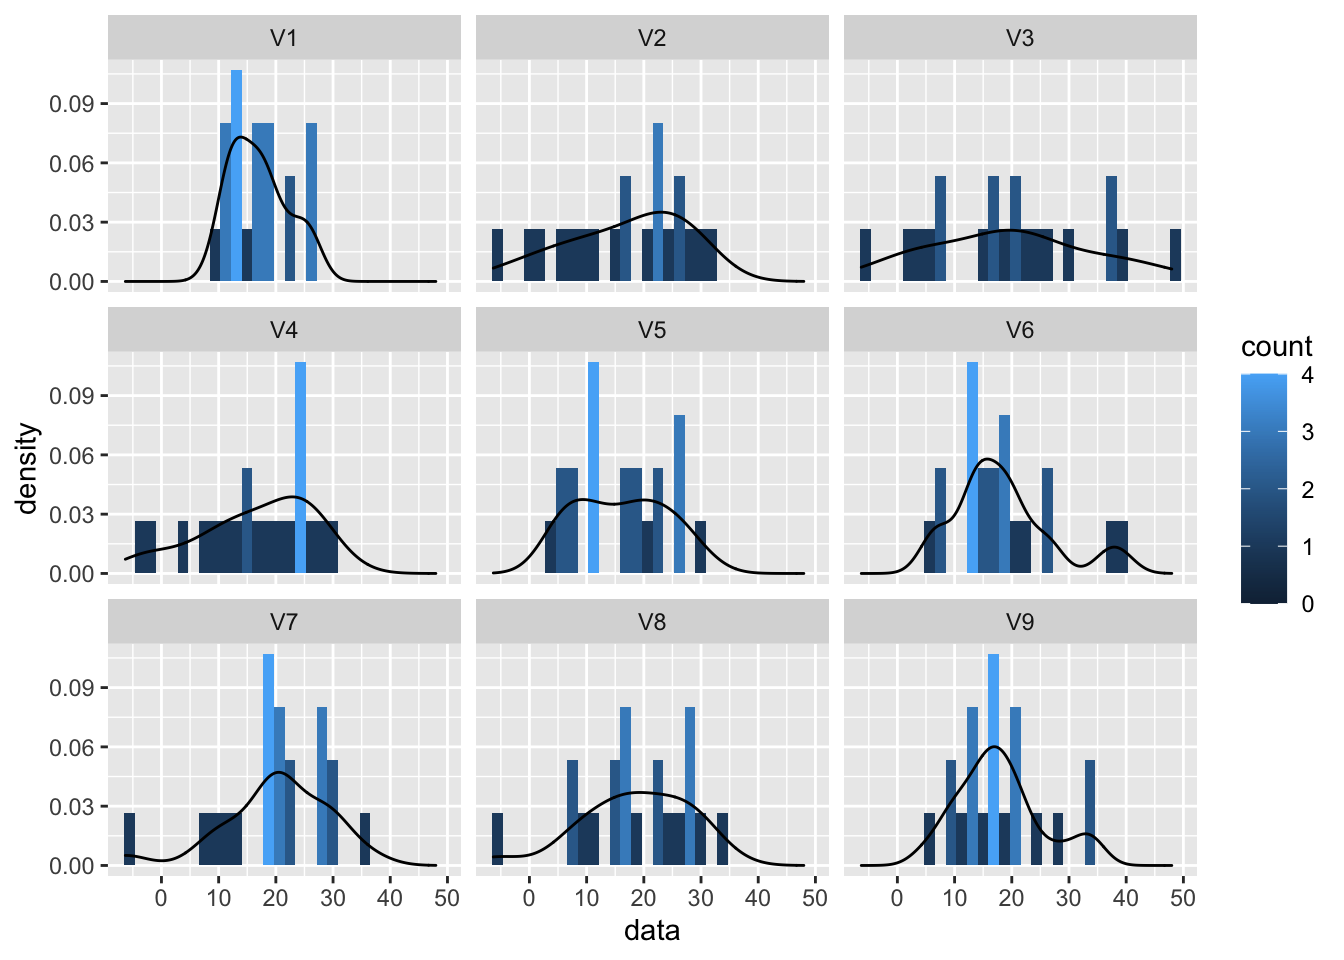
\includegraphics{Statistiek_2020_2021_files/figure-latex/unnamed-chunk-105-1.pdf}

Gezien er vrij weinig data punten zijn en omdat er veel distributies vergeleken moeten worden is het handiger om dit via een boxplot te doen.

\begin{Shaded}
\begin{Highlighting}[]
\NormalTok{normSim }\OperatorTok{\%\textgreater{}\%}\StringTok{ }\KeywordTok{gather}\NormalTok{(samp, data) }\OperatorTok{\%\textgreater{}\%}\StringTok{ }\KeywordTok{ggplot}\NormalTok{(}\KeywordTok{aes}\NormalTok{(}\DataTypeTok{x =}\NormalTok{ samp, }
    \DataTypeTok{y =}\NormalTok{ data)) }\OperatorTok{+}\StringTok{ }\KeywordTok{geom\_boxplot}\NormalTok{(}\DataTypeTok{outlier.shape =} \OtherTok{NA}\NormalTok{) }\OperatorTok{+}\StringTok{ }
\StringTok{    }\KeywordTok{geom\_point}\NormalTok{(}\DataTypeTok{position =} \StringTok{"jitter"}\NormalTok{)}
\end{Highlighting}
\end{Shaded}

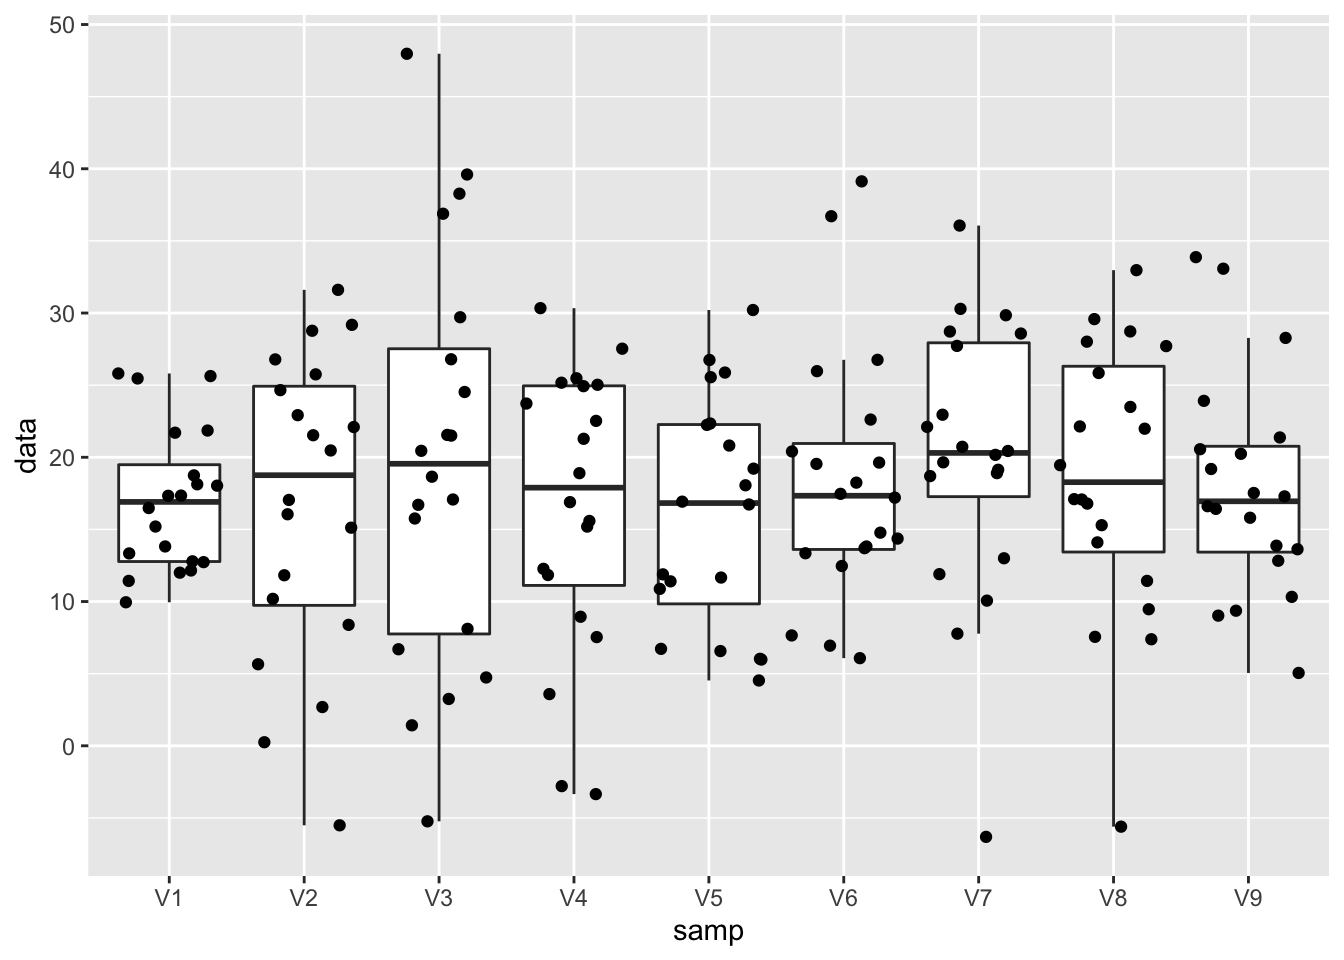
\includegraphics{Statistiek_2020_2021_files/figure-latex/unnamed-chunk-106-1.pdf}

Hoewel alle observaties in alle steekproeven uit dezelfde populatie zijn getrokken zien we toch vrij grote fluctuaties van steekproef tot steekproef in de mediaan, maar zeker ook in de boxgrootte en het bereik van de data in elke steekproef. Dus ondanks het feit dat we over een vrij grote steekproef beschikken (20 observaties) is er toch een grote variabiliteit van steekproef tot steekproef.

We gaan nu normaliteit na via QQ-plot.

\begin{enumerate}
\def\labelenumi{\arabic{enumi}.}
\tightlist
\item
  Zet data om in tidy data
\item
  maak een ggplot object
\item
  Voeg een laag toe met de QQ-plot via de functie \texttt{geom\_qq}
\item
  Voeg een laag toe met de rechte in de QQ-plot via de functie \texttt{geom\_qq\_line} om te kunnen evalueren hoe goed de data een normale verdeling volgt.
\end{enumerate}

\begin{Shaded}
\begin{Highlighting}[]
\NormalTok{normSim }\OperatorTok{\%\textgreater{}\%}\StringTok{ }\KeywordTok{gather}\NormalTok{(samp, data) }\OperatorTok{\%\textgreater{}\%}\StringTok{ }\KeywordTok{ggplot}\NormalTok{(}\KeywordTok{aes}\NormalTok{(}\DataTypeTok{sample =}\NormalTok{ data)) }\OperatorTok{+}\StringTok{ }
\StringTok{    }\KeywordTok{geom\_qq}\NormalTok{() }\OperatorTok{+}\StringTok{ }\KeywordTok{geom\_qq\_line}\NormalTok{() }\OperatorTok{+}\StringTok{ }\KeywordTok{facet\_wrap}\NormalTok{(}\OperatorTok{\textasciitilde{}}\NormalTok{samp)}
\end{Highlighting}
\end{Shaded}

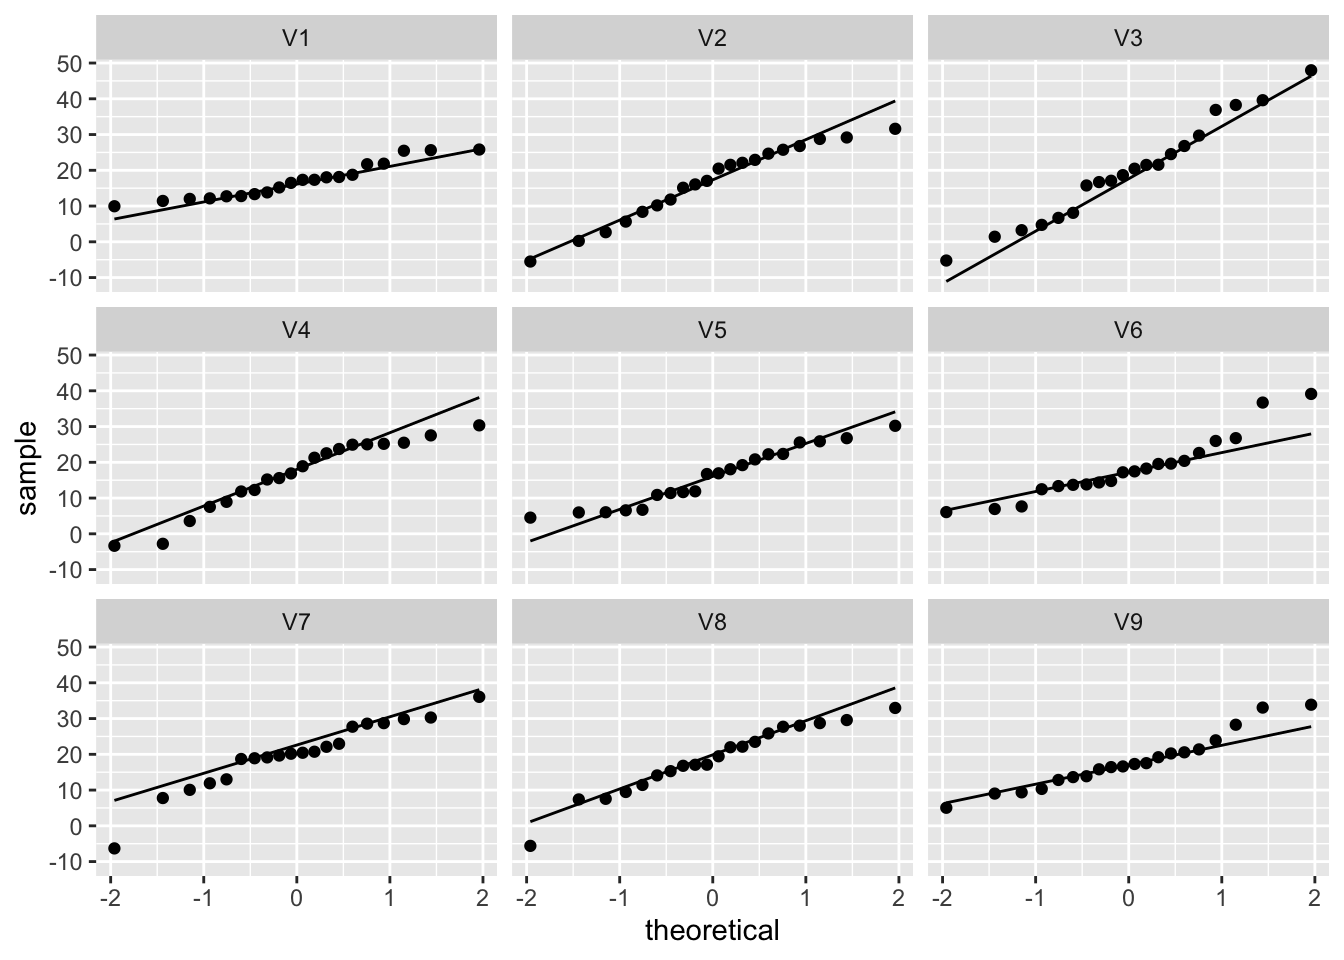
\includegraphics{Statistiek_2020_2021_files/figure-latex/unnamed-chunk-107-1.pdf}

Zelf voor Normal data zien we duidelijk nog afwijkingen door sampling variabiliteit! De plots laten ons toe om ons visueel te trainen om QQ-plots van Normale data te herkennen.

Om de interpretatie van de QQ-plot goed te kunnen illustreren gaan we een histogram en QQ-plot naast elkaar zetten.
D.m.v. het package \texttt{gridExtra} kunnen we meerdere GG-plot objecten in een matrix op dezelfde plot afbeelden.

\begin{enumerate}
\def\labelenumi{\arabic{enumi}.}
\tightlist
\item
  We maken een eerste object aan met het histogram. We slaan dit nu op als object p1 in plaats van dit te visualiseren.
\item
  Maak een object p2 met de QQ-plot
\item
  Gebruik de functie \texttt{grid.arrange} om de objecten p1 en p2 af te beelden en we geven aan dat we dit in 2 kolommen zullen doen \texttt{ncol=2}. (je kan ook de dimensie in rijen geven (nrow=1))
\end{enumerate}

\begin{Shaded}
\begin{Highlighting}[]
\KeywordTok{library}\NormalTok{(gridExtra)}
\NormalTok{p1 \textless{}{-}}\StringTok{ }\NormalTok{NHANES }\OperatorTok{\%\textgreater{}\%}\StringTok{ }\KeywordTok{filter}\NormalTok{(Gender }\OperatorTok{==}\StringTok{ "female"} \OperatorTok{\&}\StringTok{ }\OperatorTok{!}\KeywordTok{is.na}\NormalTok{(BMI)) }\OperatorTok{\%\textgreater{}\%}\StringTok{ }
\StringTok{    }\KeywordTok{ggplot}\NormalTok{(}\KeywordTok{aes}\NormalTok{(}\DataTypeTok{x =}\NormalTok{ BMI)) }\OperatorTok{+}\StringTok{ }\KeywordTok{geom\_histogram}\NormalTok{(}\KeywordTok{aes}\NormalTok{(}\DataTypeTok{y =}\NormalTok{ ..density.., }
    \DataTypeTok{fill =}\NormalTok{ ..count..)) }\OperatorTok{+}\StringTok{ }\KeywordTok{xlab}\NormalTok{(}\StringTok{"BMI"}\NormalTok{) }\OperatorTok{+}\StringTok{ }\KeywordTok{ggtitle}\NormalTok{(}\StringTok{"All females in study"}\NormalTok{) }\OperatorTok{+}\StringTok{ }
\StringTok{    }\KeywordTok{geom\_density}\NormalTok{(}\KeywordTok{aes}\NormalTok{(}\DataTypeTok{y =}\NormalTok{ ..density..))}

\NormalTok{p2 \textless{}{-}}\StringTok{ }\NormalTok{NHANES }\OperatorTok{\%\textgreater{}\%}\StringTok{ }\KeywordTok{filter}\NormalTok{(Gender }\OperatorTok{==}\StringTok{ "female"} \OperatorTok{\&}\StringTok{ }\OperatorTok{!}\KeywordTok{is.na}\NormalTok{(BMI)) }\OperatorTok{\%\textgreater{}\%}\StringTok{ }
\StringTok{    }\KeywordTok{ggplot}\NormalTok{(}\KeywordTok{aes}\NormalTok{(}\DataTypeTok{sample =}\NormalTok{ BMI)) }\OperatorTok{+}\StringTok{ }\KeywordTok{geom\_qq}\NormalTok{() }\OperatorTok{+}\StringTok{ }\KeywordTok{geom\_qq\_line}\NormalTok{()}

\KeywordTok{grid.arrange}\NormalTok{(p1, p2, }\DataTypeTok{ncol =} \DecValTok{2}\NormalTok{)}
\end{Highlighting}
\end{Shaded}

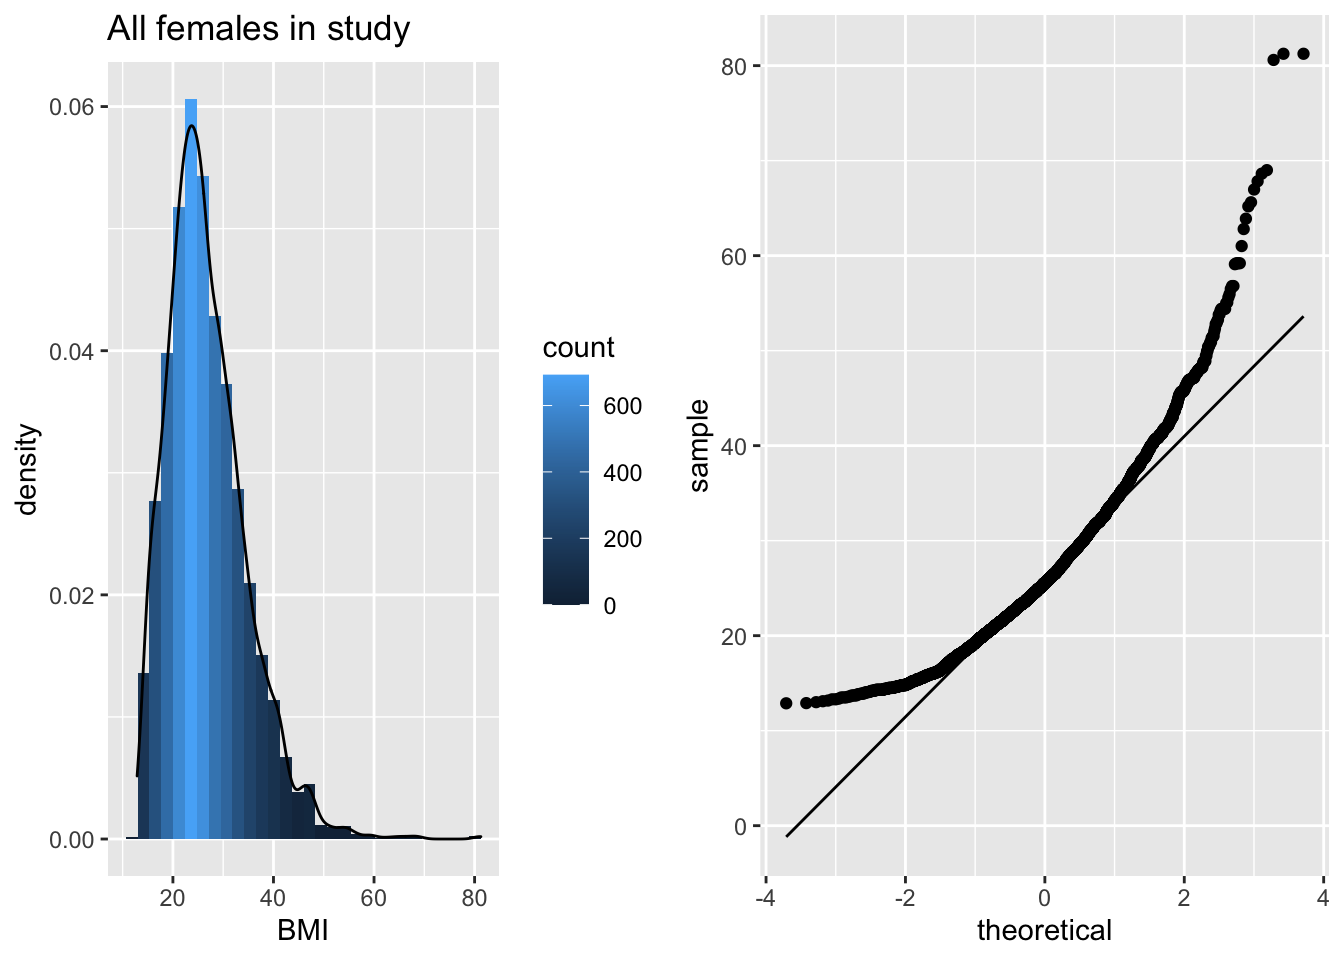
\includegraphics{Statistiek_2020_2021_files/figure-latex/unnamed-chunk-108-1.pdf}

The QQ-plot toont dat de kwantielen van de data in de steekproef

\begin{itemize}
\item
  groter zijn (boven de lijn liggen) dan wat we verwachten voor Normaal verdeelde data in de linkerstaart: compressie van de linkerstaart t.o.v. de Normale verdeling. De waarden in de linkerstaart liggen dus dichter bij top van de distributie dan wat we verwachten voor normaal verdeelde data.
\item
  groter zijn (boven de lijn liggen) dan wat we verwachten voor Normaal verdeelde data: lange staart naar rechts. De waarden in de rechterstaart liggen dus verder van de top van de distributie dan wat we verwachten voor normaal verdeelde data.
\end{itemize}

We zien dus duidelijk dat de data scheef verdeeld zijn naar rechts.

\hypertarget{sec:explCatVar}{%
\section{Samenvattingsmaten voor categorische variabelen}\label{sec:explCatVar}}

De samenvattingsmaten uit de vorige sectie (gemiddelde, mediaan, standaarddeviatie, \ldots) kunnen niet zomaar toegepast worden voor de beschrijving van categorische variabelen. In deze sectie gaan we hier dieper op in, daarbij onderscheid makend tussen enerzijds gegevens die uit prospectieve studies of lukrake steekproeven afkomstig zijn, en anderzijds gegevens uit retrospectieve studies.

\hypertarget{prospectieve-studies-en-lukrake-steekproeven}{%
\subsection{Prospectieve studies en lukrake steekproeven}\label{prospectieve-studies-en-lukrake-steekproeven}}

\begin{example}[Houtluizen]
\begin{example}

\protect\hypertarget{exm:unnamed-chunk-109}{}{\label{exm:unnamed-chunk-109} \iffalse (Houtluizen) \fi{} }

\end{example}
\end{example}

Een bioloog verzamelt `s nachts bladerafval op een lukrake plaats van 1 m\(^2\)
in 2 wouden, waarvan 1 met klei- en 1 met kalkgrond. Op elke plaats telt hij het aantal houtluizen van de species
Armadilidium of Oniscus, met als doel na te gaan of de ene soort vaker voorkomt op kleigrond dan op
kalkgrond\footnote{Merk op dat dit design niet optimaal is omdat replicaties op de verkeerde schaal werden bekomen. Idealiter moesten meer dan 2 stukken grond in de studie opgenomen worden omdat de 2 gekozen stukken grond in veel meer kunnen verschillen dan alleen het bodemtype. Verschillen in de verdeling van houtluizen kunnen bijgevolg niet zomaar aan het bodemtype kunnen toegeschreven worden.}. Tabel \ref{tab:cox} toont de bekomen gegevens. Hier stelt \(a\) (\(c\)) het aantal houtluizen van de soort Armadilidium (Oniscus) voor op kleigrond, en \(b\) (\(d\)) het aantal houtluizen van de soort Armadilidium (Oniscus) op kalkgrond.

\begin{table}[t]

\caption{\label{tab:cox}Kruistabel van species houtluis versus type grond.}
\centering
\begin{tabular}{llll}
\toprule
  & Armadil. & Oniscus & Totaal\\
\midrule
Klei & 14 (a) & 6 (c) & 20 (a+c)\\
Kalk & 22 (b) & 46 (d) & 68 (b+d)\\
Totaal & 36 (a+b) & 52 (c+d) & 88 (n)\\
\bottomrule
\end{tabular}
\end{table}

\textbf{Einde voorbeeld}

Er zijn verschillende manieren om de resultaten van deze studie te
beschrijven. De kans dat 1 van beide species houtluizen van de soort Armadilidium is, is \(p_{kl}=a/(a+c)=0.70\) of 70\% op kleigrond en \(p_{ka}=b/(b+d)=0.32\) of 32\% op kalkgrond.

\begin{definition}[absolute risico verschil]
\begin{definition}

\protect\hypertarget{def:unnamed-chunk-110}{}{\label{def:unnamed-chunk-110} \iffalse (absolute risico verschil) \fi{} }

\end{definition}
\end{definition}

Het \textbf{absolute risico verschil} of absolute kansverschil op een gegeven gebeurtenis (bvb. om Armadilidium aan te treffen) voor populatie T (Test, bvb. kleigrond) versus C (Controle, bvb. kalkgrond) wordt
met ARV genoteerd en gedefinieerd als het verschil

\begin{equation*}
ARV=p_T-p_C
\end{equation*}

tussen de kansen dat deze gebeurtenis zich voordoet in populaties T en C.

\textbf{Einde definitie}

Het ARV op Armadilidium tussen klei- en kalkgrond bedraagt 0.38, hetgeen suggereert dat de kans dat 1 van beide species houtluizen van de soort Armadilidium is, 38\% hoger is op kleigrond dan op kalkgrond. Een absoluut kansverschil
van 0 drukt uit dat de overeenkomstige kansen even groot zijn in beide
populaties en dat beide populaties dus vergelijkbaar zijn in termen van de bestudeerde uitkomst.

Het absolute kansverschil zegt echter niet alles omtrent het
bestudeerde effect. Een kansverschil kan immers een grotere impact hebben
alnaargelang beide proporties \(p_T\) en \(p_C\) dicht bij 0 of 1 liggen, dan
wanneer ze in de buurt van 0.5 liggen.
Bijvoorbeeld, wanneer we de proportie
vrouwen jonger dan 60 jaar meten die borstkanker ontwikkelen, is
een risicoverschil tussen \(p_A=0.01\) voor vrouwen die het allel Leu/Leu bezitten op het BRCA1 gen
en \(p_B=0.001\) voor de overige vrouwen, wellicht belangrijker dan een verschil tussen \(p_C=0.41\) en \(p_D=0.401\) voor beide populaties. Een uitspraak dat het risico 0.9\% lager is in de ene dan in de andere populatie geeft om die reden slechts een beperkt beeld van het belang van die reductie. Een goede vergelijking van risico's, kansen of percentages moet om die reden ook rekening houden met het basisrisico (d.w.z. de kans op de bestudeerde uitkomst in een referentiepopulatie). Het ARV doet dit niet, in tegenstelling tot volgende associatiemaat.

\begin{definition}[relatief risico]
\begin{definition}

\protect\hypertarget{def:unnamed-chunk-111}{}{\label{def:unnamed-chunk-111} \iffalse (relatief risico) \fi{} }

\end{definition}
\end{definition}

Het \textbf{relatief risico} op een gegeven gebeurtenis (bvb. om Armadilidium aan te treffen) voor populatie T (Test, bvb. kleigrond) versus C (Controle, bvb. kalkgrond) wordt met RR
genoteerd en gedefinieerd als het quotiënt

\begin{equation*}
RR=\frac{p_T}{p_C}
\end{equation*}

van de kansen dat deze gebeurtenis zich voordoet in populaties T en C.

\textbf{Einde definitie}

In de studie naar houtluizen bedraagt dit \(RR=0.70/0.32=2.2\). Dit
suggereert dat er 2.2 keer zoveel kans om een houtluis van de soort Armadilidium (i.p.v. Oniscus) aan te treffen op kleigrond dan op kalkgrond. Een
relatief risico van 1 drukt uit dat beide populaties dus vergelijkbaar zijn in termen van de bestudeerde uitkomst.

Een nadeel van het relatief risico is dat ze, in tegenstelling tot het absolute risico verschil, niet goed duidelijk maakt hoeveel meer individuen de bestudeerde uitkomst ondervinden in de ene dan in de andere populatie. Bijvoorbeeld, zelfs wetende dat het relatief risico op Armidilidium in klei-versus kalkgrond 2.2 bedraagt, is het niet mogelijk om uit te maken hoeveel meer houtluizen van de soort Armidilidium zich manifesteren op kleigrond. Als de kans om Armidilidium aan te treffen i.p.v. Oniscus 0.1\% bedraagt op kalkgrond, dan verwacht men dat er per 10000 houtluizen (van de soort Armidilidium of Oniscus) er 10 van de soort Armidilidium zullen zijn op kalkgrond en 22 op kleigrond, wat neerkomt op een verwaarloosbaar verschil van 12. Als de kans om Armidilidium aan te treffen i.p.v. Oniscus 40\% bedraagt op kalkgrond, dan verwacht men dat er per 10000 houtluizen (van de soort Armidilidium of Oniscus) er 4000 van de soort Armidilidium zullen zijn op kalkgrond en 8800 op kleigrond, wat neerkomt op een aanzienlijk verschil van 4800. Soms rapporteert men in de plaats van het relatief risico, het
\emph{relatieve risico verschil} \(ARV/p_C=RR-1\). Voor de gegeven studie
bedraagt dit 1.2. Het drukt uit dat de toename (van kalk- naar kleigrond) in kans om Armadilidium aan te treffen succes meer dan 1 keer zo groot is als het basisrisico in de controlegroep (kalkgrond).

Merk op dat alle bovenstaande associatiematen eveneens gebruikt kunnen
worden wanneer men, in tegenstelling tot wat in een prospectieve studie
gebeurt, een volledig lukrake groep proefpersonen selecteert zonder vast te
leggen hoeveel van hen al dan niet blootgesteld zijn.

\hypertarget{subsec:retrospect}{%
\subsection{Retrospectieve studies}\label{subsec:retrospect}}

Beschouw de case-controle studie uit Voorbeeld \ref{exm:brcaLeu}, waarvan
de gegevens samengevat zijn in Tabel \ref{tab:leu2}. Omdat men in
zo'n design op zoek gaat naar \(a+b+c\) lukraak gekozen controles en \(d+e+f\) lukraak
gekozen cases, liggen de marges \(a+b+c\) en \(d+e+f\) vast en is het bijgevolg
onmogelijk om het risico op case (bvb. risico op borstkanker) te schatten. Dit is noch mogelijk binnen de
totale groep, noch binnen de groep van blootgestelden (d.i. vrouwen met allel Leu/Leu), noch binnen de groep
niet-blootgestelden. Immers, de kans op case binnen die geobserveerde groep reflecteert hoofdzakelijk de verhouding waarin cases en controles in totaal werden gekozen door het design. Alleen analyses die de kolomtotalen
in de tabel vast gegeven veronderstellen, zijn hier zinvol. Dit heeft tot
gevolg dat \emph{het relatief risico} op de aandoening (d.w.z. op \emph{case})
in de populatie voor blootgestelden versus niet-blootgestelden niet
rechtstreeks kan geschat worden op basis van gegevens uit een \emph{case-controle studie}. Analoog kan ook het bijhorende \emph{absolute risicoverschil niet geschat} worden.

\begin{table}[t]

\caption{\label{tab:leu2}Kruistabel van borstkanker-status versus BRCA1-allel.}
\centering
\begin{tabular}{llll}
\toprule
Genotype & Controles & Cases & Totaal\\
\midrule
Pro/Pro & 266 (a) & 342 (d) & 608 (a+d)\\
Pro/Leu & 250 (b) & 369 (e) & 619 (b+e)\\
Leu/Leu & 56 (c) & 89 (f) & 145 (c+f)\\
Totaal & 572 (a+b+c) & 800 (d+e+f) & 1372 (n)\\
\bottomrule
\end{tabular}
\end{table}

Wel heeft men informatie over de kans om het allel Leu/Leu aan te treffen bij cases, \(\pi_1=f/(d+e+f)=89/800=11.1\%\), en de kans op het allel Leu/Leu bij controles, \(\pi_0=c/(a+b+c)=56/572=9.8\%\). Het relatief risico op blootstelling voor cases versus
controles is bijgevolg \(11.1/9.8=1.14\). Vrouwen met borstkanker hebben dus
14\% meer kans om de allelcombinatie Leu/Leu te hebben op het BRCA1 gen dan vrouwen zonder borstkanker.
Dit suggereert dat er
een associatie\footnote{Al is het nog de vraag of die associatie toevallig is, dan wel systematisch. We komen in het hoofdstuk \ref{chap:categorisch}. terug op technieken om dit te onderzoeken.} is tussen het polymorfisme op het BRCA1 gen en borstkanker, maar drukt helaas niet uit hoeveel hoger het risico op borstkanker is voor vrouwen met de allelcombinatie Leu/Leu dan voor andere vrouwen. Om toch een antwoord te vinden op deze laatste vraag, voeren we een nieuwe risicomaat in.

\begin{definition}[Odds]
\begin{definition}

\protect\hypertarget{def:unnamed-chunk-112}{}{\label{def:unnamed-chunk-112} \iffalse (Odds) \fi{} }

\end{definition}
\end{definition}

De \emph{odds} op een gebeurtenis wordt gedefinieerd als

\begin{equation*}
\frac{p}{1-p}
\end{equation*}

waarbij \(p\) de kans is op die gebeurtenis.

\textbf{Einde definitie}

De odds is dus een transformatie van het risico, met onder andere de
volgende eigenschappen:

\begin{itemize}
\item
  de odds neemt waarden aan tussen nul en oneindig.
\item
  de odds is gelijk aan 1 als en slechts als de kans zelf gelijk is aan
  1/2.
\item
  de odds neemt toe als de kans toeneemt.
\end{itemize}

Het gebruik van odds is populair onder gokkers omdat het uitdrukt hoeveel
waarschijnlijker het is om te winnen dan om te verliezen. Een odds op winnen
gelijk aan 1 drukt bijvoorbeeld uit dat het even waarschijnlijk is om te
winnen dan om te verliezen. Een odds op winnen gelijk aan 0.9 drukt uit men
per 10 verliesbeurten, 9 keer verwacht te winnen. In de genetische associatiestudie uit Voorbeeld \ref{exm:brcaLeu}
is de odds op allel Leu/Leu bij cases gelijk aan
\(\mbox{odds}_1=f/(d+e)=89/711=0.125\) en bij controles gelijk aan \(\mbox{odds}_2=c/(a+b)=56/516=0.109\). Vrouwen met borstkanker hebben bijgevolg ongeveer 8 (\(\approx 1/0.125\)) keer meer kans om de allelcombinatie Leu/Leu niet te hebben op het BRCA1 gen dan om het wel te hebben.
Om de associatie tussen blootstelling
en uitkomst te beschrijven, kan men nu een verhouding van odds (odds ratio)
gebruiken in plaats van een verhouding van risico's (relatief risico).

\begin{definition}[Odds ratio]
\begin{definition}

\protect\hypertarget{def:unnamed-chunk-113}{}{\label{def:unnamed-chunk-113} \iffalse (Odds ratio) \fi{} }

\end{definition}
\end{definition}

De \textbf{odds ratio} op een gegeven gebeurtenis (bvb. borstkanker) voor populatie T (bvb. vrouwen met allel Leu/Leu) versus C (bvb. vrouwen zonder allel Leu/Leu) wordt met OR genoteerd en gedefinieerd als het quotiënt
\begin{equation*}
OR=\frac{\mbox{odds}_T}{\mbox{odds}_C}
\end{equation*}
van de odds op deze gebeurtenis in populaties T en C.

\textbf{Einde definitie}

Op basis van de gegevens in Tabel \ref{tab:leu2} kan de odds ratio op
blootstelling voor cases versus controles geschat worden d.m.v. het kruisproduct

\begin{equation*}
\frac{ \frac{ f/(d+e+f)}{(d+e)/(d+e+f)} }{ \frac{c/(a+b+c)}{(a+b)/(a+b+c)}} = \frac{f(a+b)}{c (d+e)}
\end{equation*}

In het bijzonder vinden we dat de odds op allelcombinatie Leu/Leu voor vrouwen met versus zonder borstkanker gelijk is aan \(OR=(89\times 516)/(56\times 711)=1.15\). Helaas drukt dit resultaat nog steeds
niet uit hoeveel meer risico op borstkanker vrouwen met de allelcombinatie Leu/Leu lopen.

Was de bovenstaande studie echter een volledig lukrake steekproef geweest
(waarbij het aantal cases en controles niet per design werden vastgelegd),
dan konden we daar ook de odds ratio op borstkanker berekenen voor mensen
met versus zonder het allel Leu/leu. We zouden dan vaststellen dat dit gelijk is
aan

\begin{equation*}
\frac{ \frac{ f/(c+f)}{c/(c+f)} }{ \frac{(d+e)/(a+b+d+e)}{(a+b)/(a+b+d+e)}} = \frac{f(a+b)}{c(d+e)},
\end{equation*}

en bijgevolg dezelfde waarde aanneemt. Dat is omdat de odds ratio een
\emph{symmetrische associatiemaat} is zodat de odds ratio op `case' voor
blootgestelden versus niet-blootgestelden steeds gelijk is aan de odds op
blootstelling voor cases versus controles. Hieruit volgt dat voor het
schatten van de odds ratio het er niet toe doet of we prospectief werken
zoals in een typische cohort studie, of retrospectief zoals in een typische
case-controle studie. In het bijzonder kunnen we in de genetische associatiestudie uit
Voorbeeld \ref{exm:brcaLeu} de odds op borstkanker voor vrouwen met allel Leu/leu
versus zonder berekenen als \(OR=89\times 516/(56\times 711)=1.15\).
De odds op borstkanker is bijgevolg 15\% hoger bij vrouwen met die specifieke allelcombinatie.

Stel nu dat we met \(p_T\) en \(p_C\) respectievelijk de kans op case noteren
voor blootgestelden en niet-blootgestelden. Wanneer beide kansen klein zijn
(namelijk \(p_T<5\%\) en \(p_C<5\%\)), dan is de odds een goede benadering voor
het risico. Dit is omdat in dat geval \(\mbox{odds}_T=p_T/(1-p_T)\approx p_T\) en \(\mbox{odds}_C=p_C/(1-p_C)\approx p_C\). Er volgt dan bovendien dat de odds ratio
een goede benadering voor het relatief risico:

\begin{equation*}
OR=\frac{\mbox{ odds}_T}{\mbox{
odds}_C}\approx \frac{p_T}{p_C}=RR
\end{equation*}

Wetende dat het risico op borstkanker laag is, mogen we
op basis van de gevonden OR van 1.15 bijgevolg
besluiten dat het risico (i.p.v. de odds) op borstkanker (bij benadering) 15\% hoger ligt bij vrouwen met het allel Leu/Leu op het BRCA1 gen. Dit is een bijzonder
nuttige eigenschap omdat (a) het relatief risico, dat niet rechtstreeks
geschat kan worden in case-controle studies, gemakkelijker te interpreteren
is dan de odds ratio; en (b) de odds ratio bepaalde wiskundige eigenschappen
heeft die ze aantrekkelijker maakt dan een relatief risico in statistische
modellen\footnote{Dit is bijvoorbeeld het geval in logistische regressiemodellen die gebruikt worden om het
  risico op een bepaalde aandoening te modelleren in functie van prognostische
  factoren.}. Algemeen is de odds ratio echter steeds verder van 1 verwijderd
dan het relatief risico. Wetende dat de odds ratio op borstkanker 1.15
bedraagt voor vrouwen met versus zonder de allelcombinatie Leu/Leu, kunnen we bijgevolg meer
nauwkeurig besluiten dat het overeenkomstige relatief risico tussen 1 en 1.15
gelegen is (maar niettemin dicht bij 1.15).

Omdat de odds ratio moeilijker te interpreteren is dan een relatief risico
en bijgevolg misleidend kan zijn, valt deze laatste steeds te verkiezen in
situaties (zoals prospectieve studies) waar het mogelijk is om het relatief
risico in de populatie te schatten. In sommige case-controle studies (nl.
matched case-controle studies) wordt voor elke case een controle gezocht die
bepaalde karakteristieken gemeenschappelijk heeft, teneinde een betere
onderlinge vergelijkbaarheid te garanderen. In dat geval moet de
statistische analyse (inclusief de manier om odds ratio's te schatten)
rekening houden met het feit dat de resultaten van elke case gecorreleerd of
verwant zijn met de resultaten van de bijhorende controle.

\hypertarget{rates-versus-risicos}{%
\subsection{Rates versus risico's}\label{rates-versus-risicos}}

Vaak wordt het begrip \emph{risico} verward met het begrip \emph{rate}. Een
\emph{rate} drukt een aantal gebeurtenissen (bvb. aantal sterfte- of
ziektegevallen) uit per eenheid in de populatie in een bepaalde tijdspanne.
Bijvoorbeeld, een \emph{crude mortality rate (CMR)} voor een bepaald
jaartal is gedefinieerd als 1000 maal het aantal sterftegevallen dat
optreedt in dat jaar gedeeld door de grootte van de beschouwde populatie
halfweg dat jaar. De reden dat met 1000 wordt vermenigvuldigd is dat het
bijvoorbeeld makkelijker na te denken is over een CMR van 12 sterftes per
1000 in Engeland en Wales, dan over 0.012 sterftes per individu. Indien een
specifieke leeftijdsgroep wordt gekozen, verkrijgt men de \emph{leeftijdsspecifieke mortality rate} als 1000 maal het aantal sterftegevallen
dat optreedt in een bepaald jaar en bepaalde leeftijdsgroep gedeeld door de
grootte van de beschouwde populatie in die leeftijdsklasse halfweg dat jaar.
In tegenstelling tot de incidentie, is de prevalentie geen rate omdat ze
niet een aantal gebeurtenissen uitdrukt over een zekere tijdspanne.

\hypertarget{associaties-tussen-twee-variabelen}{%
\section{Associaties tussen twee variabelen}\label{associaties-tussen-twee-variabelen}}

Tot nog toe zijn we hoofdzakelijk ingegaan op zogenaamde univariate beschrijvingen waarbij slechts 1 variabele onderzocht wordt. In de meeste wetenschappelijke studies wenst men echter associaties tussen 2 of meerdere variabelen te onderzoeken, bijvoorbeeld tussen een interventie en de daarop volgende respons. In deze Sectie onderzoeken we hoe associaties tussen 2 variabelen kunnen beschreven worden. We maken daarbij onderscheid naargelang het type van de variabelen.

\hypertarget{subsec:kruistabel}{%
\subsection{Associatie tussen twee kwalitatieve variabelen}\label{subsec:kruistabel}}

Als twee kwalitatieve variabelen niet veel verschillende waarden aannemen,
dan is een \emph{kruistabel} aangewezen om hun associatie voor te stellen.
In deze tabel worden de verschillende waarden die de ene variabele aanneemt
in de kolommen uitgezet en de verschillende waarden die de andere variabele
aanneemt in de rijen. In elke cel van de tabel (die overeenkomt met 1
specifieke combinatie van waarden voor beide variabelen) wordt de frequentie
neergeschreven.

\begin{table}[t]

\caption{\label{tab:genderBMI}Kruistabel van Gender vs BMI klasse.}
\centering
\begin{tabular}{lrrrr}
\toprule
  & 12.0\_18.5 & 18.5\_to\_24.9 & 25.0\_to\_29.9 & 30.0\_plus\\
\midrule
female & 629 & 1616 & 1179 & 1402\\
male & 648 & 1295 & 1485 & 1349\\
\bottomrule
\end{tabular}
\end{table}

Tabel \ref{tab:genderBMI} toont zo'n kruistabel voor het aantal mannen en vrouwen per BMI klasse. Dergelijke eenvoudige kruistabel met slechts 2 rijen en 4 kolommen, noemt men ook een \(2\times 4\) tabel.

\hypertarget{subsec:asskwalcont}{%
\subsection{Associatie tussen één kwalitatieve en één continue variabele}\label{subsec:asskwalcont}}

Boxplots zijn meer compact dan een histogram en laat om die reden gemakkelijker vergelijkingen tussen verschillende groepen toe. Twee dergelijke boxplots
worden getoond in Figuur \ref{fig:boxplotCholGender}.

\begin{Shaded}
\begin{Highlighting}[]
\NormalTok{NHANES }\OperatorTok{\%\textgreater{}\%}\StringTok{ }\KeywordTok{ggplot}\NormalTok{(}\KeywordTok{aes}\NormalTok{(}\DataTypeTok{x =}\NormalTok{ Gender, }\DataTypeTok{y =} \KeywordTok{log}\NormalTok{(DirectChol))) }\OperatorTok{+}\StringTok{ }
\StringTok{    }\KeywordTok{geom\_boxplot}\NormalTok{() }\OperatorTok{+}\StringTok{ }\KeywordTok{ylab}\NormalTok{(}\StringTok{"log(Direct Cholestorol)"}\NormalTok{)}
\end{Highlighting}
\end{Shaded}

\begin{figure}

{\centering 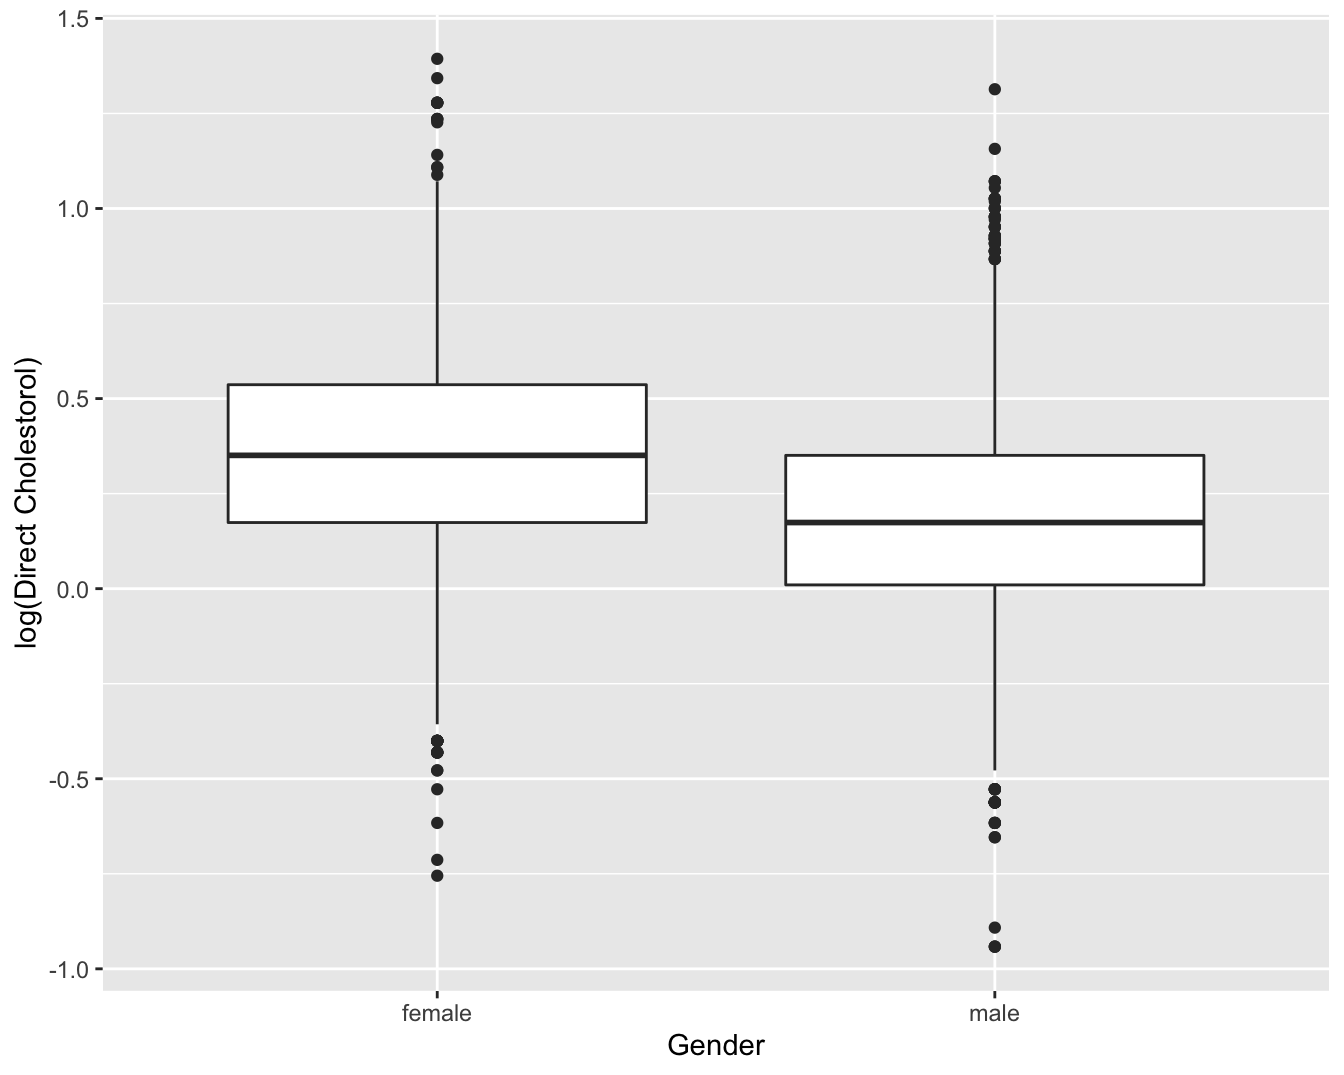
\includegraphics[width=1\linewidth]{Statistiek_2020_2021_files/figure-latex/boxplotCholGender-1} 

}

\caption{Boxplot van log-getransformeerde directe HDL cholestorol concentratie in functie van Gender voor alle subjecten van de NHANES studie.}\label{fig:boxplotCholGender}
\end{figure}

Op basis van deze figuur
stellen we vast dat hogere log-cholestorol concentraties
geobserveerd worden bij vrouwen dan bij mannen, maar dat de variabiliteit
van de log-concentraties vergelijkbaar is tussen de 2 groepen. De vraag blijft of we hier kunnen spreken van een systematisch hogere
log-cholestorol concentratie tussen vrouwen en mannen. We zullen in Hoofdstuk \ref{chap:besluit} dieper op deze vraag ingaan.

Figuur \ref{fig:boxplotCholGender} kan men samenvatten door gemiddelde verschillen tussen beide groepen te rapporteren. Hier stellen we een gemiddeld verschil van 0.17 in directe HDL cholestorol concentratie vast op de log schaal tussen vrouwen en mannen.
Gezien we weten dat \(\log(C_2)-\log(C_1)=\log(C_2/C_1)\) weten we dat de HDL cholestorol concentratie in de NHANES studie gemiddeld 1.19 keer hoger ligt voor vrouwen dan voor mannen.

In de introductie hebben we bij het microbiome voorbeeld gezien dat het ook erg nuttig is om de ruwe data weer te geven op de boxplot. Als het aantal gegevens niet te hoog is kunnen we eenvoudig een extra laag toevoegen met de originele datapunten. Merk op dat het wel belangrijk is om de outliers dan niet weer te geven in de boxplot, anders zal men deze twee keer afbeelden. Eens in de geom\_boxplot laag een eens in de geom\_point laag. Daarom zetten we het symbool voor de outliers op NA.

In onderstaande grafiek plotten we de relatieve abundanties van \textbf{Staphylococcus} van de oksel microbiome case study.

\begin{enumerate}
\def\labelenumi{\arabic{enumi}.}
\tightlist
\item
  We pipen het \texttt{ap} dataframe naar \texttt{ggplot}
\item
  We selecteren de data voor de plot via \texttt{ggplot(aes(x=trt,y=rel))}
\item
  We voegen laag toe voor de boxplot dmv de functie \texttt{geom\_boxplot()}. Merk op dat we het argument \texttt{outlier.shape} op NA (not available) zetten \texttt{outlier.shape=NA} in the \texttt{geom\_boxplot} functie omdat we anders outliers twee keer weer zullen geven. Eerst via de boxplot laag en daarna omdat we een laag met alle ruwe data toevoegen aan de plot.
\item
  We geven de ruwe data weer via de \texttt{geom\_point(position="jitter")} functie. We gebruiken hierbij het argument position=`jitter' zodat we wat random ruis toevoegen aan de x-cordinaat zodat de gegevens elkaar niet overlappen.
\end{enumerate}

\begin{Shaded}
\begin{Highlighting}[]
\NormalTok{ap \textless{}{-}}\StringTok{ }\KeywordTok{read\_csv}\NormalTok{(}\StringTok{"https://raw.githubusercontent.com/GTPB/PSLS20/master/data/armpit.csv"}\NormalTok{)}

\NormalTok{ap }\OperatorTok{\%\textgreater{}\%}\StringTok{ }\KeywordTok{ggplot}\NormalTok{(}\KeywordTok{aes}\NormalTok{(}\DataTypeTok{x =}\NormalTok{ trt, }\DataTypeTok{y =}\NormalTok{ rel)) }\OperatorTok{+}\StringTok{ }\KeywordTok{geom\_boxplot}\NormalTok{(}\DataTypeTok{outlier.shape =} \OtherTok{NA}\NormalTok{) }\OperatorTok{+}\StringTok{ }
\StringTok{    }\KeywordTok{geom\_point}\NormalTok{(}\DataTypeTok{position =} \StringTok{"jitter"}\NormalTok{)}
\end{Highlighting}
\end{Shaded}

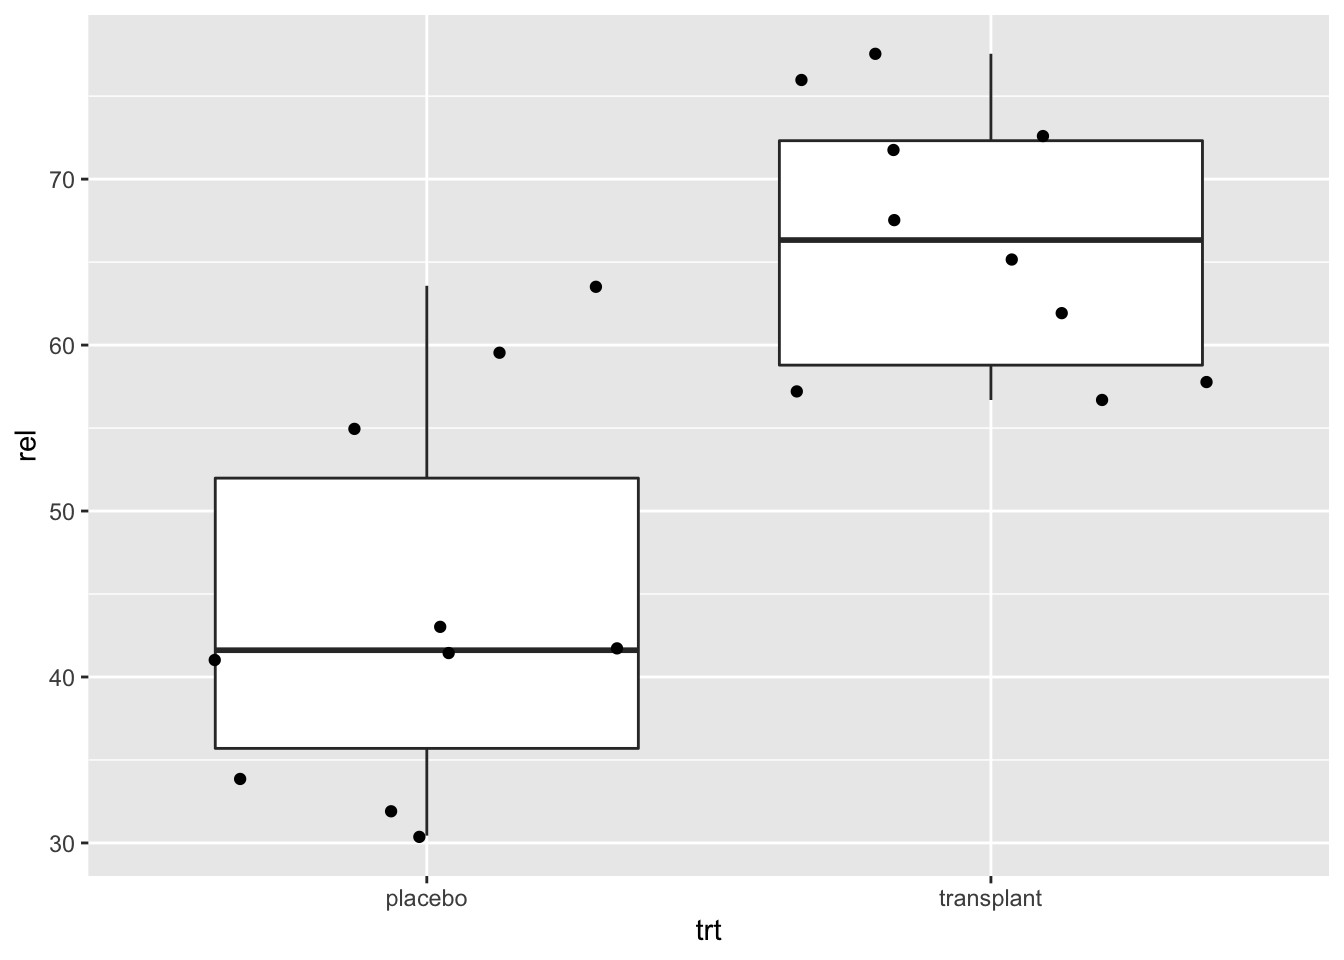
\includegraphics{Statistiek_2020_2021_files/figure-latex/unnamed-chunk-114-1.pdf}

Dot-plots zijn bijzonder interessant in pre-test post-test designs waar dezelfde subjecten op
verschillende tijdstippen worden geobserveerd. In dat geval kunnen de uitkomsten
uitgezet worden op de Y-as en de tijdstippen op de X-as, en kunnen de
metingen voor eenzelfde subject worden verbonden met een lijn.

Een
voorbeeld hiervan is weergegeven in Figuur \ref{fig:captoDot}. De figuur vat de gegevens samen van de captopril studie die de centrale dataset vormt van Hoofdstuk \ref{chap:besluit}. In de studie wenst men het effect van een bloeddrukverlagend geneesmiddel captopril evalueren. Voor elke patiënt in de studie werd de systolische bloeddruk twee keer gemeten: één keer voor en één keer na de behandeling met het bloeddruk verlagende medicijn captopril. In Figuur \ref{fig:captoDot} worden de metingen van dezelfde patiënt met een lijntje verbonden. Hierdoor krijgen we een heel duidelijk beeld van de gegevens. Namelijk, we krijgen een sterke indruk dat de bloeddruk daalt na het toedienen van captopril gezien we bijna voor alle patiënten een daling observeren.

\begin{Shaded}
\begin{Highlighting}[]
\CommentTok{\# Eerst lezen we de data in. Deze bevindt zich in}
\CommentTok{\# de subdirectory dataset Het is een tekstbestand}
\CommentTok{\# waarbij de kolommen van elkaar gescheiden zijn}
\CommentTok{\# d.m.v comma\textquotesingle{}s. sep=\textquotesingle{},\textquotesingle{} De eerste rij bevat de}
\CommentTok{\# namen van de variabelen}
\NormalTok{captopril \textless{}{-}}\StringTok{ }\KeywordTok{read.table}\NormalTok{(}\StringTok{"https://raw.githubusercontent.com/statOmics/sbc20/master/data/captopril.txt"}\NormalTok{, }
    \DataTypeTok{header =} \OtherTok{TRUE}\NormalTok{, }\DataTypeTok{sep =} \StringTok{","}\NormalTok{)}
\KeywordTok{head}\NormalTok{(captopril)}
\end{Highlighting}
\end{Shaded}

\begin{verbatim}
##   id SBPb DBPb SBPa DBPa
## 1  1  210  130  201  125
## 2  2  169  122  165  121
## 3  3  187  124  166  121
## 4  4  160  104  157  106
## 5  5  167  112  147  101
## 6  6  176  101  145   85
\end{verbatim}

\begin{Shaded}
\begin{Highlighting}[]
\NormalTok{captoprilTidy \textless{}{-}}\StringTok{ }\NormalTok{captopril }\OperatorTok{\%\textgreater{}\%}\StringTok{ }\KeywordTok{gather}\NormalTok{(type, bp, }\OperatorTok{{-}}\NormalTok{id)}

\NormalTok{captoprilTidy }\OperatorTok{\%\textgreater{}\%}\StringTok{ }\KeywordTok{filter}\NormalTok{(type }\OperatorTok{\%in\%}\StringTok{ }\KeywordTok{c}\NormalTok{(}\StringTok{"SBPa"}\NormalTok{, }\StringTok{"SBPb"}\NormalTok{)) }\OperatorTok{\%\textgreater{}\%}\StringTok{ }
\StringTok{    }\KeywordTok{mutate}\NormalTok{(}\DataTypeTok{type =} \KeywordTok{factor}\NormalTok{(type, }\DataTypeTok{levels =} \KeywordTok{c}\NormalTok{(}\StringTok{"SBPb"}\NormalTok{, }\StringTok{"SBPa"}\NormalTok{))) }\OperatorTok{\%\textgreater{}\%}\StringTok{ }
\StringTok{    }\KeywordTok{ggplot}\NormalTok{(}\KeywordTok{aes}\NormalTok{(}\DataTypeTok{x =}\NormalTok{ type, }\DataTypeTok{y =}\NormalTok{ bp)) }\OperatorTok{+}\StringTok{ }\KeywordTok{geom\_line}\NormalTok{(}\KeywordTok{aes}\NormalTok{(}\DataTypeTok{group =}\NormalTok{ id)) }\OperatorTok{+}\StringTok{ }
\StringTok{    }\KeywordTok{geom\_point}\NormalTok{()}
\end{Highlighting}
\end{Shaded}

\begin{figure}

{\centering 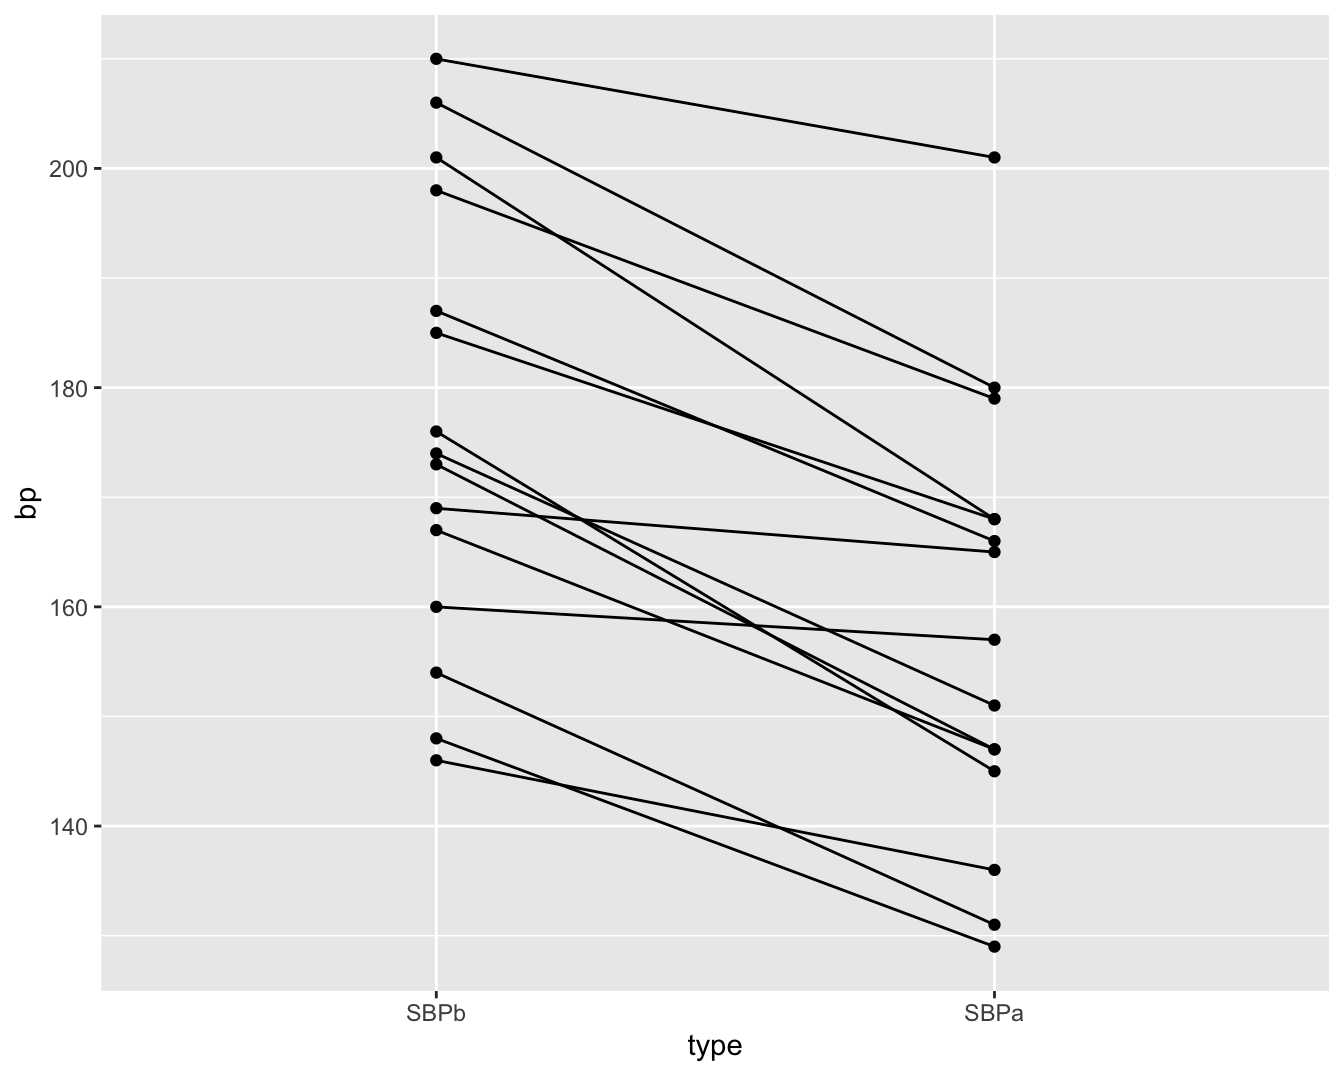
\includegraphics[width=1\linewidth]{Statistiek_2020_2021_files/figure-latex/captoDot-1} 

}

\caption{Dotplot van de systolische bloeddruk in de captopril studie voor en na het toedienen van het bloeddruk verlagend middel captopril.}\label{fig:captoDot}
\end{figure}

\hypertarget{associatie-tussen-twee-continue-variabelen}{%
\section{Associatie tussen twee continue variabelen}\label{associatie-tussen-twee-continue-variabelen}}

We zullen dit opnieuw illustreren aan de hand van de NHANES studie. We bestuderen hierbij lengte en gewicht bij vrouwen.

We voeren eerst een data exploratie uit waarbij we

\begin{enumerate}
\def\labelenumi{\arabic{enumi}.}
\tightlist
\item
  De volwassen vrouwen filteren uit de dataset
\item
  In het ggplot commando de lengte selecteren in de x-as en het gewicht in de y-as.
\item
  Een laag toevoegen d.m.v. \texttt{geom\_point} om een scatterplot te bekomen van y i.f.v. x.
\end{enumerate}

\begin{Shaded}
\begin{Highlighting}[]
\NormalTok{NHANES }\OperatorTok{\%\textgreater{}\%}\StringTok{ }\KeywordTok{filter}\NormalTok{(Age }\OperatorTok{\textgreater{}=}\StringTok{ }\DecValTok{18} \OperatorTok{\&}\StringTok{ }\NormalTok{Gender }\OperatorTok{==}\StringTok{ "female"}\NormalTok{) }\OperatorTok{\%\textgreater{}\%}\StringTok{ }
\StringTok{    }\KeywordTok{ggplot}\NormalTok{(}\KeywordTok{aes}\NormalTok{(}\DataTypeTok{x =}\NormalTok{ Height, }\DataTypeTok{y =}\NormalTok{ Weight)) }\OperatorTok{+}\StringTok{ }\KeywordTok{geom\_point}\NormalTok{()}
\end{Highlighting}
\end{Shaded}

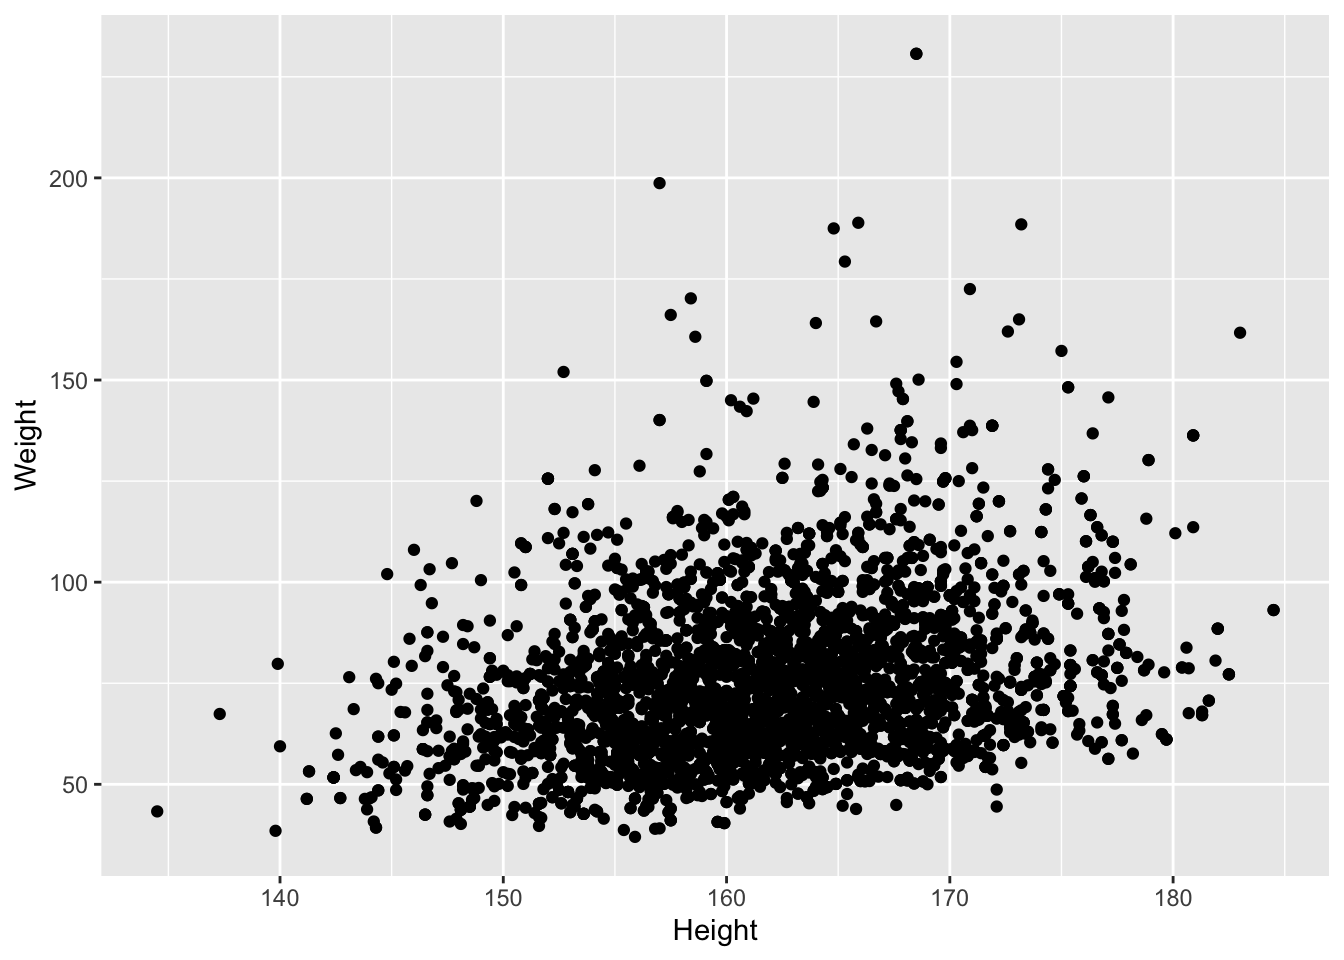
\includegraphics{Statistiek_2020_2021_files/figure-latex/unnamed-chunk-115-1.pdf}

Er is een duidelijke associatie tussen gewicht en lengte: als de lengte stijgt dan stijgt het gewicht gemiddeld ook. Er is echter veel variabiliteit en ook een indicatie dat het gewicht is scheef verdeeld naar rechts.

We exploreren eerst de data univariaat: variabele per variabele. Om een histogram en QQ-plot naast elkaar af te beelden slaan we de plots eerst op als een object en maken we gebruik van de \texttt{grid.arrange} functie van het gridExtra package om de plots naast elkaar te plotten.

\begin{Shaded}
\begin{Highlighting}[]
\NormalTok{p1 \textless{}{-}}\StringTok{ }\NormalTok{NHANES }\OperatorTok{\%\textgreater{}\%}\StringTok{ }\KeywordTok{filter}\NormalTok{(Age }\OperatorTok{\textgreater{}=}\StringTok{ }\DecValTok{18} \OperatorTok{\&}\StringTok{ }\NormalTok{Gender }\OperatorTok{==}\StringTok{ "female"}\NormalTok{) }\OperatorTok{\%\textgreater{}\%}\StringTok{ }
\StringTok{    }\KeywordTok{ggplot}\NormalTok{(}\KeywordTok{aes}\NormalTok{(}\DataTypeTok{x =}\NormalTok{ Height)) }\OperatorTok{+}\StringTok{ }\KeywordTok{geom\_histogram}\NormalTok{(}\KeywordTok{aes}\NormalTok{(}\DataTypeTok{y =}\NormalTok{ ..density.., }
    \DataTypeTok{fill =}\NormalTok{ ..count..)) }\OperatorTok{+}\StringTok{ }\KeywordTok{xlab}\NormalTok{(}\StringTok{"Height"}\NormalTok{) }\OperatorTok{+}\StringTok{ }\KeywordTok{ggtitle}\NormalTok{(}\StringTok{"All females in study"}\NormalTok{) }\OperatorTok{+}\StringTok{ }
\StringTok{    }\KeywordTok{geom\_density}\NormalTok{(}\KeywordTok{aes}\NormalTok{(}\DataTypeTok{y =}\NormalTok{ ..density..))}

\NormalTok{p2 \textless{}{-}}\StringTok{ }\NormalTok{NHANES }\OperatorTok{\%\textgreater{}\%}\StringTok{ }\KeywordTok{filter}\NormalTok{(Age }\OperatorTok{\textgreater{}=}\StringTok{ }\DecValTok{18} \OperatorTok{\&}\StringTok{ }\NormalTok{Gender }\OperatorTok{==}\StringTok{ "female"}\NormalTok{) }\OperatorTok{\%\textgreater{}\%}\StringTok{ }
\StringTok{    }\KeywordTok{ggplot}\NormalTok{(}\KeywordTok{aes}\NormalTok{(}\DataTypeTok{sample =}\NormalTok{ Height)) }\OperatorTok{+}\StringTok{ }\KeywordTok{geom\_qq}\NormalTok{() }\OperatorTok{+}\StringTok{ }\KeywordTok{geom\_qq\_line}\NormalTok{()}
\KeywordTok{grid.arrange}\NormalTok{(p1, p2, }\DataTypeTok{ncol =} \DecValTok{2}\NormalTok{)}
\end{Highlighting}
\end{Shaded}

\includegraphics{Statistiek_2020_2021_files/figure-latex/unnamed-chunk-116-1.pdf}

De lengte data zijn duidelijk approximatief normaal verdeeld.

\begin{Shaded}
\begin{Highlighting}[]
\NormalTok{p3 \textless{}{-}}\StringTok{ }\NormalTok{NHANES }\OperatorTok{\%\textgreater{}\%}\StringTok{ }\KeywordTok{filter}\NormalTok{(Age }\OperatorTok{\textgreater{}=}\StringTok{ }\DecValTok{18} \OperatorTok{\&}\StringTok{ }\NormalTok{Gender }\OperatorTok{==}\StringTok{ "female"}\NormalTok{) }\OperatorTok{\%\textgreater{}\%}\StringTok{ }
\StringTok{    }\KeywordTok{ggplot}\NormalTok{(}\KeywordTok{aes}\NormalTok{(}\DataTypeTok{x =}\NormalTok{ Weight)) }\OperatorTok{+}\StringTok{ }\KeywordTok{geom\_histogram}\NormalTok{(}\KeywordTok{aes}\NormalTok{(}\DataTypeTok{y =}\NormalTok{ ..density.., }
    \DataTypeTok{fill =}\NormalTok{ ..count..)) }\OperatorTok{+}\StringTok{ }\KeywordTok{xlab}\NormalTok{(}\StringTok{"Weight"}\NormalTok{) }\OperatorTok{+}\StringTok{ }\KeywordTok{ggtitle}\NormalTok{(}\StringTok{"All females in study"}\NormalTok{) }\OperatorTok{+}\StringTok{ }
\StringTok{    }\KeywordTok{geom\_density}\NormalTok{(}\KeywordTok{aes}\NormalTok{(}\DataTypeTok{y =}\NormalTok{ ..density..))}

\NormalTok{p4 \textless{}{-}}\StringTok{ }\NormalTok{NHANES }\OperatorTok{\%\textgreater{}\%}\StringTok{ }\KeywordTok{filter}\NormalTok{(Age }\OperatorTok{\textgreater{}=}\StringTok{ }\DecValTok{18} \OperatorTok{\&}\StringTok{ }\NormalTok{Gender }\OperatorTok{==}\StringTok{ "female"}\NormalTok{) }\OperatorTok{\%\textgreater{}\%}\StringTok{ }
\StringTok{    }\KeywordTok{ggplot}\NormalTok{(}\KeywordTok{aes}\NormalTok{(}\DataTypeTok{sample =}\NormalTok{ Weight)) }\OperatorTok{+}\StringTok{ }\KeywordTok{geom\_qq}\NormalTok{() }\OperatorTok{+}\StringTok{ }\KeywordTok{geom\_qq\_line}\NormalTok{()}

\KeywordTok{grid.arrange}\NormalTok{(p3, p4, }\DataTypeTok{ncol =} \DecValTok{2}\NormalTok{)}
\end{Highlighting}
\end{Shaded}

\includegraphics{Statistiek_2020_2021_files/figure-latex/unnamed-chunk-117-1.pdf}

De gewichtsdata zijn inderdaad scheef verdeeld!

Na log transformatie zijn de gewichtsdata minder scheef, maar nog steeds niet Normaal verdeeld.

\begin{Shaded}
\begin{Highlighting}[]
\NormalTok{p5 \textless{}{-}}\StringTok{ }\NormalTok{NHANES }\OperatorTok{\%\textgreater{}\%}\StringTok{ }\KeywordTok{filter}\NormalTok{(Age }\OperatorTok{\textgreater{}=}\StringTok{ }\DecValTok{18} \OperatorTok{\&}\StringTok{ }\NormalTok{Gender }\OperatorTok{==}\StringTok{ "female"}\NormalTok{) }\OperatorTok{\%\textgreater{}\%}\StringTok{ }
\StringTok{    }\KeywordTok{ggplot}\NormalTok{(}\KeywordTok{aes}\NormalTok{(}\DataTypeTok{x =}\NormalTok{ Weight }\OperatorTok{\%\textgreater{}\%}\StringTok{ }\NormalTok{log2)) }\OperatorTok{+}\StringTok{ }\KeywordTok{geom\_histogram}\NormalTok{(}\KeywordTok{aes}\NormalTok{(}\DataTypeTok{y =}\NormalTok{ ..density.., }
    \DataTypeTok{fill =}\NormalTok{ ..count..)) }\OperatorTok{+}\StringTok{ }\KeywordTok{xlab}\NormalTok{(}\StringTok{"Weight (log2)"}\NormalTok{) }\OperatorTok{+}\StringTok{ }\KeywordTok{ggtitle}\NormalTok{(}\StringTok{"All females in study"}\NormalTok{) }\OperatorTok{+}\StringTok{ }
\StringTok{    }\KeywordTok{geom\_density}\NormalTok{(}\KeywordTok{aes}\NormalTok{(}\DataTypeTok{y =}\NormalTok{ ..density..))}

\NormalTok{p6 \textless{}{-}}\StringTok{ }\NormalTok{NHANES }\OperatorTok{\%\textgreater{}\%}\StringTok{ }\KeywordTok{filter}\NormalTok{(Age }\OperatorTok{\textgreater{}=}\StringTok{ }\DecValTok{18} \OperatorTok{\&}\StringTok{ }\NormalTok{Gender }\OperatorTok{==}\StringTok{ "female"}\NormalTok{) }\OperatorTok{\%\textgreater{}\%}\StringTok{ }
\StringTok{    }\KeywordTok{ggplot}\NormalTok{(}\KeywordTok{aes}\NormalTok{(}\DataTypeTok{sample =}\NormalTok{ Weight }\OperatorTok{\%\textgreater{}\%}\StringTok{ }\NormalTok{log2)) }\OperatorTok{+}\StringTok{ }\KeywordTok{geom\_qq}\NormalTok{() }\OperatorTok{+}\StringTok{ }
\StringTok{    }\KeywordTok{geom\_qq\_line}\NormalTok{()}

\KeywordTok{grid.arrange}\NormalTok{(p5, p6, }\DataTypeTok{ncol =} \DecValTok{2}\NormalTok{)}
\end{Highlighting}
\end{Shaded}

\includegraphics{Statistiek_2020_2021_files/figure-latex/unnamed-chunk-118-1.pdf}

De scheefheid is er nog maar is sterk gereduceerd. We maken nu een plot van lengte in functie van het log\(_2\) getransformeerde gewicht.

\begin{Shaded}
\begin{Highlighting}[]
\NormalTok{NHANES }\OperatorTok{\%\textgreater{}\%}\StringTok{ }\KeywordTok{filter}\NormalTok{(Age }\OperatorTok{\textgreater{}=}\StringTok{ }\DecValTok{18} \OperatorTok{\&}\StringTok{ }\NormalTok{Gender }\OperatorTok{==}\StringTok{ "female"}\NormalTok{) }\OperatorTok{\%\textgreater{}\%}\StringTok{ }
\StringTok{    }\KeywordTok{ggplot}\NormalTok{(}\KeywordTok{aes}\NormalTok{(}\DataTypeTok{x =}\NormalTok{ Height, }\DataTypeTok{y =}\NormalTok{ Weight }\OperatorTok{\%\textgreater{}\%}\StringTok{ }\NormalTok{log2)) }\OperatorTok{+}\StringTok{ }
\StringTok{    }\KeywordTok{ylab}\NormalTok{(}\StringTok{"Weight (log2)"}\NormalTok{) }\OperatorTok{+}\StringTok{ }\KeywordTok{geom\_point}\NormalTok{()}
\end{Highlighting}
\end{Shaded}

\includegraphics{Statistiek_2020_2021_files/figure-latex/unnamed-chunk-119-1.pdf}

We introduceren nu een statistiek om de associatie te schatten: de correlatie.

\hypertarget{covariantie-en-correlatie}{%
\subsection{Covariantie en Correlatie}\label{covariantie-en-correlatie}}

Stel dat X en Y continue toevallig veranderlijken zijn

\begin{itemize}
\tightlist
\item
  Voor elk subject i observeren we dus \((X_i,Y_i)\).
\item
  Covariantie: hoe variëren \(X_i\) en \(Y_i\) rond hun gemiddelde \((E[X],E[Y])\)?
\end{itemize}

\[\mbox{Covar}(X,Y)=E[(X-E[X])(Y-E[Y])]\]

\begin{itemize}
\tightlist
\item
  De covariantie is dus de verwachte waarde van het product van de afwijking van de X waarde t.o.v. zijn verwachte waarde E{[}X{]} en de afwijking van de Y waarde t.o.v.zijn verwachte waarde E{[}Y{]}.
\end{itemize}

We kunnen de covariantie nu ook standardiseren zodat we een maat krijgen die voor elke dataset vergelijkbaar wordt: de correlatie. We doen dit door de covariantie te delen door de standaardafwijking van elke variabele:

\[\mbox{Cor}(X,Y)=\frac{E[(X-E[X])(Y-E[Y])]}{\sqrt{E[(X-E[X])^2}\sqrt{E[(Y-E[Y])^2}}\]

\hypertarget{pearson-correlatie}{%
\subsection{Pearson Correlatie}\label{pearson-correlatie}}

We introduceren nu een schatter voor de correlatie tussen twee continue toevallig veranderlijken op basis van de data in de steekproef:

\[
\mbox{Cor}(X,Y)=\frac{\sum_{i=1}^{n}(x_{i}-\bar{x})(y_{i}-\bar{y})}{(n-1)s_{x}s_{y}}
\]

We vervangen de verwachte waarden weer door het steekproefgemiddelden \(\bar x\) en \(\bar y\), en, we berekenen het gemiddeld product van de afwijkingen in x en y in de steekproef. Let op dat we hierbij weer corrigeren voor het aantal vrijheidsgraden. We geven elke observatie geen gewicht van 1/n maar van 1/(n-1). We hebben inderdaad het gemiddelde geschat, hier is dat gemiddelde bivariaat (het heeft een x en y coordinaat).

Deze schatter wordt ook wel de Pearson correlatie genoemd en heeft volgende eigenschappen:

\begin{itemize}
\item
  Er is een positieve correlatie wanneer \(y\) gemiddeld toeneemt bij een toename van: \(x \ \nearrow \ \Rightarrow \ y \ \nearrow\)
\item
  Er is een negatieve correlatie als \(y\) gemiddeld afneemt bij een toename in \(x\): \(x \ \nearrow \ \Rightarrow \ y \ \searrow\)
\item
  De correlatie ligt ook altijd tussen -1 en 1
\end{itemize}

In de figuur \ref{fig:bijdrageCor} wordt de bijdrage weergegeven van individuele metingen in de correlatie. Als punten in het 1ste en 3de kwadrant liggen is er een negatieve bijdrage van de observatie in de correlatie, als ze in het 2de en 4de kwadrant liggen is er een positieve bijdrage.

\begin{figure}
\centering
\includegraphics{Statistiek_2020_2021_files/figure-latex/bijdrageCor-1.pdf}
\caption{\label{fig:bijdrageCor}Bijdrage van individuele metingen in de correlatie.}
\end{figure}

We berekenen vervolgens de correlatie voor lengte, gewicht en het log getransformeerde gewicht.

\begin{Shaded}
\begin{Highlighting}[]
\NormalTok{NHANES }\OperatorTok{\%\textgreater{}\%}\StringTok{ }\KeywordTok{filter}\NormalTok{(Age }\OperatorTok{\textgreater{}=}\StringTok{ }\DecValTok{18} \OperatorTok{\&}\StringTok{ }\NormalTok{Gender }\OperatorTok{==}\StringTok{ "female"}\NormalTok{) }\OperatorTok{\%\textgreater{}\%}\StringTok{ }
\StringTok{    }\KeywordTok{select}\NormalTok{(Weight, Height) }\OperatorTok{\%\textgreater{}\%}\StringTok{ }\KeywordTok{mutate}\NormalTok{(}\DataTypeTok{log2Weight =}\NormalTok{ Weight }\OperatorTok{\%\textgreater{}\%}\StringTok{ }
\StringTok{    }\NormalTok{log2) }\OperatorTok{\%\textgreater{}\%}\StringTok{ }\NormalTok{na.exclude }\OperatorTok{\%\textgreater{}\%}\StringTok{ }\NormalTok{cor}
\end{Highlighting}
\end{Shaded}

\begin{verbatim}
##               Weight    Height log2Weight
## Weight     1.0000000 0.2845792  0.9811638
## Height     0.2845792 1.0000000  0.3074578
## log2Weight 0.9811638 0.3074578  1.0000000
\end{verbatim}

Merk op dat:

\begin{itemize}
\tightlist
\item
  De correlatie lager is als de data niet worden getransformeerd.
\item
  De Pearson correlatie is gevoelig voor outliers!
\item
  Gebruik de Pearson correlatie niet voor scheef verdeelde data of data met outliers!
\end{itemize}

\hypertarget{impact-van-outliers}{%
\subsubsection{Impact van outliers}\label{impact-van-outliers}}

In figuur \ref{fig:corOutlier} wordt de impact van outliers op de Pearson correlatie geïllustreerd d.m.v. gesimuleerde data met één outlier. We zien dat de correlatie bijna halveert ten gevolge van de outlier!

\begin{Shaded}
\begin{Highlighting}[]
\KeywordTok{set.seed}\NormalTok{(}\DecValTok{100}\NormalTok{)}
\NormalTok{x \textless{}{-}}\StringTok{ }\KeywordTok{rnorm}\NormalTok{(}\DecValTok{20}\NormalTok{)}
\NormalTok{simData \textless{}{-}}\StringTok{ }\KeywordTok{data.frame}\NormalTok{(}\DataTypeTok{x =}\NormalTok{ x, }\DataTypeTok{y =}\NormalTok{ x }\OperatorTok{*}\StringTok{ }\DecValTok{2} \OperatorTok{+}\StringTok{ }\KeywordTok{rnorm}\NormalTok{(}\KeywordTok{length}\NormalTok{(x)))}
\NormalTok{p1 \textless{}{-}}\StringTok{ }\NormalTok{simData }\OperatorTok{\%\textgreater{}\%}\StringTok{ }\KeywordTok{ggplot}\NormalTok{(}\KeywordTok{aes}\NormalTok{(}\DataTypeTok{x =}\NormalTok{ x, }\DataTypeTok{y =}\NormalTok{ y)) }\OperatorTok{+}\StringTok{ }\KeywordTok{geom\_point}\NormalTok{() }\OperatorTok{+}\StringTok{ }
\StringTok{    }\KeywordTok{ggtitle}\NormalTok{(}\KeywordTok{paste}\NormalTok{(}\StringTok{"cor ="}\NormalTok{, }\KeywordTok{cor}\NormalTok{(simData[, }\DecValTok{1}\NormalTok{], simData[, }
        \DecValTok{2}\NormalTok{]) }\OperatorTok{\%\textgreater{}\%}\StringTok{ }\KeywordTok{round}\NormalTok{(., }\DecValTok{2}\NormalTok{)))}

\NormalTok{outlier \textless{}{-}}\StringTok{ }\KeywordTok{rbind}\NormalTok{(simData, }\KeywordTok{c}\NormalTok{(}\DecValTok{2}\NormalTok{, }\DecValTok{{-}4}\NormalTok{))}
\NormalTok{p2 \textless{}{-}}\StringTok{ }\NormalTok{outlier }\OperatorTok{\%\textgreater{}\%}\StringTok{ }\KeywordTok{ggplot}\NormalTok{(}\KeywordTok{aes}\NormalTok{(}\DataTypeTok{x =}\NormalTok{ x, }\DataTypeTok{y =}\NormalTok{ y)) }\OperatorTok{+}\StringTok{ }\KeywordTok{geom\_point}\NormalTok{() }\OperatorTok{+}\StringTok{ }
\StringTok{    }\KeywordTok{ggtitle}\NormalTok{(}\KeywordTok{paste}\NormalTok{(}\StringTok{"cor ="}\NormalTok{, }\KeywordTok{cor}\NormalTok{(outlier[, }\DecValTok{1}\NormalTok{], outlier[, }
        \DecValTok{2}\NormalTok{]) }\OperatorTok{\%\textgreater{}\%}\StringTok{ }\KeywordTok{round}\NormalTok{(., }\DecValTok{2}\NormalTok{)))}

\KeywordTok{grid.arrange}\NormalTok{(p1, p2, }\DataTypeTok{ncol =} \DecValTok{2}\NormalTok{)}
\end{Highlighting}
\end{Shaded}

\begin{figure}
\centering
\includegraphics{Statistiek_2020_2021_files/figure-latex/corOutlier-1.pdf}
\caption{\label{fig:corOutlier}Correlatie van gesimuleerde data met 1 outlier}
\end{figure}

\hypertarget{de-pearson-correlatie-pikt-enkel-linear-associatie-op}{%
\subsubsection{De Pearson correlatie pikt enkel linear associatie op}\label{de-pearson-correlatie-pikt-enkel-linear-associatie-op}}

In figuur \ref{fig:corQuad} simuleren we data met een kwadratisch verband en observeren we dat de correlatie bijna nul is!

\begin{Shaded}
\begin{Highlighting}[]
\NormalTok{x \textless{}{-}}\StringTok{ }\KeywordTok{rnorm}\NormalTok{(}\DecValTok{100}\NormalTok{)}
\NormalTok{quadratic \textless{}{-}}\StringTok{ }\KeywordTok{data.frame}\NormalTok{(}\DataTypeTok{x =}\NormalTok{ x, }\DataTypeTok{y =}\NormalTok{ x}\OperatorTok{\^{}}\DecValTok{2} \OperatorTok{+}\StringTok{ }\KeywordTok{rnorm}\NormalTok{(}\KeywordTok{length}\NormalTok{(x)))}
\NormalTok{quadratic }\OperatorTok{\%\textgreater{}\%}\StringTok{ }\KeywordTok{ggplot}\NormalTok{(}\KeywordTok{aes}\NormalTok{(}\DataTypeTok{x =}\NormalTok{ x, }\DataTypeTok{y =}\NormalTok{ y)) }\OperatorTok{+}\StringTok{ }\KeywordTok{geom\_point}\NormalTok{() }\OperatorTok{+}\StringTok{ }
\StringTok{    }\KeywordTok{ggtitle}\NormalTok{(}\KeywordTok{paste}\NormalTok{(}\StringTok{"cor ="}\NormalTok{, }\KeywordTok{cor}\NormalTok{(quadratic[, }\DecValTok{1}\NormalTok{], quadratic[, }
        \DecValTok{2}\NormalTok{]) }\OperatorTok{\%\textgreater{}\%}\StringTok{ }\KeywordTok{round}\NormalTok{(., }\DecValTok{2}\NormalTok{))) }\OperatorTok{+}\StringTok{ }\KeywordTok{geom\_hline}\NormalTok{(}\DataTypeTok{yintercept =} \KeywordTok{mean}\NormalTok{(quadratic[, }
    \DecValTok{2}\NormalTok{]), }\DataTypeTok{col =} \StringTok{"red"}\NormalTok{) }\OperatorTok{+}\StringTok{ }\KeywordTok{geom\_vline}\NormalTok{(}\DataTypeTok{xintercept =} \KeywordTok{mean}\NormalTok{(quadratic[, }
    \DecValTok{1}\NormalTok{]), }\DataTypeTok{col =} \StringTok{"red"}\NormalTok{)}
\end{Highlighting}
\end{Shaded}

\begin{figure}
\centering
\includegraphics{Statistiek_2020_2021_files/figure-latex/corQuad-1.pdf}
\caption{\label{fig:corQuad}Correlatie van gesimuleerde data met een kwadratisch verband. De data in de bovenste kwadranten compenseren elkaar als het ware alsook in de onderste kwadranten (ongeveer evenveel positieve en negatieve bijdragen door de data in de correlatie)}
\end{figure}

\hypertarget{verschillende-groottes-van-correlatie}{%
\subsection{Verschillende groottes van correlatie}\label{verschillende-groottes-van-correlatie}}

Om een inzicht te krijgen in de grootte van de correlatie, simuleren we data met een verschillende correlatie. We geven telkens de correlatie weer boven de plot. Hoe sterker de correlatie hoe meer de puntenwolk naar een lineair verband toegaat.

\includegraphics{Statistiek_2020_2021_files/figure-latex/unnamed-chunk-121-1.pdf} \includegraphics{Statistiek_2020_2021_files/figure-latex/unnamed-chunk-121-2.pdf}

\hypertarget{spearman-correlatie}{%
\subsection{Spearman correlatie}\label{spearman-correlatie}}

De Spearman correlatie is de Pearson correlatie na transformatie van de data naar ranks. Hierdoor wordt deze schatter minder gevoelig voor outliers.

\begin{itemize}
\tightlist
\item
  Pearson correlatie
\end{itemize}

\begin{Shaded}
\begin{Highlighting}[]
\KeywordTok{cor}\NormalTok{(outlier)}
\end{Highlighting}
\end{Shaded}

\begin{verbatim}
##           x         y
## x 1.0000000 0.4682823
## y 0.4682823 1.0000000
\end{verbatim}

\begin{itemize}
\tightlist
\item
  Spearman correlatie
\end{itemize}

\begin{Shaded}
\begin{Highlighting}[]
\KeywordTok{cor}\NormalTok{(outlier, }\DataTypeTok{method =} \StringTok{"spearman"}\NormalTok{)}
\end{Highlighting}
\end{Shaded}

\begin{verbatim}
##           x         y
## x 1.0000000 0.6571429
## y 0.6571429 1.0000000
\end{verbatim}

We verifiëren dat de Spearman correlatie de Pearson correlatie is van rang getransformeerde data. Die wordt bekomen door de observaties te ordenen van klein naar groot en elke observatie te vervangen door zijn rangorde.

\begin{Shaded}
\begin{Highlighting}[]
\NormalTok{rankData \textless{}{-}}\StringTok{ }\KeywordTok{apply}\NormalTok{(outlier, }\DecValTok{2}\NormalTok{, rank)}
\KeywordTok{cor}\NormalTok{(rankData)}
\end{Highlighting}
\end{Shaded}

\begin{verbatim}
##           x         y
## x 1.0000000 0.6571429
## y 0.6571429 1.0000000
\end{verbatim}

We berekenen nu de Spearman correlatie in de NHANES studie.
We observeren dat de correlatie tussen lengte en gewicht, en lengte en log2 getransformeerd gewicht exact gelijk is.
Dat is logisch want de log-transformatie is een monotone transformatie en verandert de ordening van de data dus niet, de ranks van gewicht en deze van het log gewicht zijn identiek!

\begin{Shaded}
\begin{Highlighting}[]
\NormalTok{NHANES }\OperatorTok{\%\textgreater{}\%}\StringTok{ }\KeywordTok{filter}\NormalTok{(Age }\OperatorTok{\textgreater{}=}\StringTok{ }\DecValTok{18} \OperatorTok{\&}\StringTok{ }\NormalTok{Gender }\OperatorTok{==}\StringTok{ "female"}\NormalTok{) }\OperatorTok{\%\textgreater{}\%}\StringTok{ }
\StringTok{    }\KeywordTok{select}\NormalTok{(Weight, Height) }\OperatorTok{\%\textgreater{}\%}\StringTok{ }\KeywordTok{mutate}\NormalTok{(}\DataTypeTok{log2Weight =}\NormalTok{ Weight }\OperatorTok{\%\textgreater{}\%}\StringTok{ }
\StringTok{    }\NormalTok{log2) }\OperatorTok{\%\textgreater{}\%}\StringTok{ }\NormalTok{na.exclude }\OperatorTok{\%\textgreater{}\%}\StringTok{ }\KeywordTok{cor}\NormalTok{(}\DataTypeTok{method =} \StringTok{"spearman"}\NormalTok{)}
\end{Highlighting}
\end{Shaded}

\begin{verbatim}
##               Weight    Height log2Weight
## Weight     1.0000000 0.2892776  1.0000000
## Height     0.2892776 1.0000000  0.2892776
## log2Weight 1.0000000 0.2892776  1.0000000
\end{verbatim}

Bij het interpreteren van correlaties, alsook bij het uitvoeren van
regressie-analyses in de volgende secties, zijn de volgende waarschuwingen
van zeer groot belang:

\begin{enumerate}
\def\labelenumi{\arabic{enumi}.}
\item
  Correlaties zijn het makkelijkst te interpreteren tussen 2 groepen Normaal verdeelde observaties. Een kleine training laat immers toe om snel inzicht te krijgen in de grootte van de correlatiecoëfficiënt zonder zich verder over de specifieke verdeling te hoeven bekommeren. In het bijzonder kan men voor Normaal verdeelde observaties visueel inzicht krijgen in de sterkte van de correlatie door een ellips rond de puntenwolk te tekenen die (nagenoeg) alle punten bevat. Als de ellips op een cirkel lijkt, dan is er geen correlatie. Hoe dunner de ellips, hoe sterker de correlatie. De oriëntatie van de ellips geeft hierbij het teken van de correlatie weer.
\item
  Voor niet-Normale gegevens hangt de betekenis van een correlatiecoëfficiënt van zekere grootte, nauw samen met de specifieke vorm van de verdeling. Wanneer de 2 variabelen die we onderzoeken niet Normaal verdeeld zijn, dan zijn er 2 mogelijkheden om een zinvolle correlatiecoëfficiënt weer te geven. Variabelen die scheef verdeeld zijn, kan men transformeren (bvb. een log-transformatie) in de hoop dat de getransformeerde gegevens bij benadering Normaal verdeeld zijn en lineair samenhangen.
\item
  Merk op dat een correlatiecoëfficiënt van 0 tussen 2 variabelen \(X\) en \(Y\) niet noodzakelijk impliceert dat deze variabelen onafhankelijk zijn. Zie kwadratisch verband! Daarom is het van belang om de aard van samenhang tussen 2 variabelen steeds te onderzoeken via een scatterplot alvorens een correlatiecoëfficiënt te rapporteren. Wanneer het verband monotoon is, maar sterk niet-lineair is, dan is het aangewezen om niet de Pearson correlatiecoëfficiënt, maar Spearman's correlatiecoëfficiënt te rapporteren. Indien het verband niet-monotoon is, dan zijn correlatiecoëfficiënten niet geschikt en moet men overstappen op meer geavanceerde regressietechnieken.
\item
  Bij jonge kinderen is de grootte van hun schoenmaat uiteraard sterk gecorreleerd met hun leescapaciteiten. Dat op zich impliceert echter niet dat het leren van nieuwe woorden hun voeten doet groeien of dat het groeien van hun voeten impliceert dat ze beter kunnen lezen. Ook algemeen\footnote{In het Engels is dit welbekend onder de zinsnede \emph{`Association is not causation!'}.} hoeft een correlatie tussen 2 variabelen niet te impliceren dat er een causaal verband is. De relatie tussen 2 metingen kan immers sterk verstoord worden door confounders (bvb. de leeftijd in bovenstaand voorbeeld). Hoewel dit overduidelijk is in bovenstaand voorbeeld, is het in vele andere contexten veel minder duidelijk en worden er, vooral in de populaire literatuur, vaak causale beweringen gemaakt die niet (volledig) door de gegevens worden gestaafd. Volgend voorbeeld illustreert dit. Denk hierbij aan het voorbeeld van de associatie van groente consumptie en covid mortaliteit.
\item
  Een \emph{ecologische analyse} is een statistische analyse waarbij men associaties bestudeert tussen samenvattingsmaten (zoals gemiddelden, incidenties, \ldots) die reeds berekend werden voor groepen subjecten. Dit is het geval bij het covid voorbeeld uit de introductie waarbij men mortaliteit modellereert in functie van de gemiddelde dagelijkse groenteconsumptie per capita in verschillende landen. Wanneer men aldus een \emph{ecologische correlatie} vaststelt voor groepen subjecten of individuen (in dit geval,landen), impliceert dat niet noodzakelijk dat deze correlatie ook voor de subjecten zelf opgaat\footnote{In het Engels is dit welbekend onder de naam \emph{`ecological fallacy'}.}. Volgend voorbeeld illustreert dit.
\end{enumerate}

\begin{example}[Ecological fallacy]
\begin{example}

\protect\hypertarget{exm:unnamed-chunk-126}{}{\label{exm:unnamed-chunk-126} \iffalse (Ecological fallacy) \fi{} }

\end{example}
\end{example}

Voor de 48 staten in de V.S. werden telkens 2 getallen
berekend: het percentage van de mensen die in een ander land geboren zijn en het percentage geletterden. De correlatie ertussen bedraagt 0.53 (Robinson, 1950). Dit is een \emph{ecologische correlatie} omdat de eenheid van de analyse de groep residenten uit een zelfde staat is, en niet de individuele residenten zelf. Deze ecologische correlatie suggereert dat mensen van vreemde afkomst doorgaans beter geschoold zijn (in Amerikaans Engels) dan de oorspronkelijke inwoners. Wanneer men echter de correlatie berekent op basis
van de gegevens voor alle individuele residenten, bekomt men -0.11. De ecologische analyse is hier duidelijk misleidend: het teken van de correlatie is er positief omdat mensen van vreemde origine de neiging hebben om te gaan wonen in staten waar de oorspronkelijke bevolking relatief goed geschoold is.

\textbf{Einde voorbeeld}

\hypertarget{sec:missing}{%
\section{Onvolledige gegevens}\label{sec:missing}}

Het gebeurt vaak in de biowetenschappen dat, ondanks zorgvuldig veld- en laboratoriumwerk, metingen die men plande te verzamelen, niet bekomen werden. Men noemt deze dan \emph{ontbrekende gegevens} of \emph{missing data (points)}.

Minder drastisch, kunnen observaties soms slechts ten dele gekend zijn.
Bijvoorbeeld bij een studie van de overlevingsduur van dieren en planten wacht men niet steeds tot
alle subjecten gestorven zijn. Op het eind van de studie zal men bijvoorbeeld voor een 50-jarige
olifant die in leven is, slechts weten dat de overlevingstijd
minstens 50 jaar bedraagt, maar niet de exacte waarde kennen. Zo'n gegeven
wordt \emph{rechts-gecensureerd} genoemd: we weten dat de gewenste
observatie rechts van 50 ligt, maar verder niets meer.

Analoog kunnen observaties \emph{links-gecensureerd} zijn. Bij het meten
van bepaalde concentraties kan een detectielimiet bestaan: een ondergrens beneden
dewelke het meettoestel geen aanwezigheid kan detecteren. Men weet in zo'n
geval dat de concentratie kleiner dan die ondergrens is, maar niet hoeveel
kleiner.

Tenslotte vermelden we nog \emph{interval-gecensureerde} gegevens. Bij het
screenen naar HIV bijvoorbeeld, zal men weten dat een subject seropositief
geworden is ergens tussen de laatste negatieve HIV test en de eerste
positieve HIV test, maar het exacte tijdstip van seroconversie blijft
onbekend.

De aanwezigheid van gegevens die niet of slechts partieel zijn opgemeten zorgt
altijd voor extra moeilijkheden bij de analyse en interpretatie van de
onderzoeksresultaten. Dat is omdat de missende gegevens mogelijks afkomstig zijn
van een speciale populatie. Dat is het meest duidelijk in klinische experimenten bij mensen.
Patiënten zullen hier vaak de studie verlaten wanneer
ze genezen zijn, in welk geval men de metingen van deze patiënten niet te
zien krijgt. Dit negeren door enkel de aanwezige gegevens te analyseren, zal
de resultaten er slechter doen uitzien dan ze in werkelijkheid zijn. Meestal
houdt dat immers de veronderstelling in dat de aanwezige gegevens representatief blijven
voor de populatie die men wenst te bestuderen. Dit kan in sommige gevallen
de resultaten sterk vertekenen. In de statistische literatuur zijn de
laatste jaren heel wat complexe technieken ontwikkeld om hiervoor te
corrigeren. Deze technieken worden meer en meer in de statistische software
ingebouwd en recent heeft ook R verschillende bibliotheken toegevoegd.
Het is
echter aangewezen om voor het gebruik van deze gevorderde technieken een
statisticus te consulteren.

\hypertarget{clips-over-de-code-in-dit-hoofdstuk}{%
\section{Clips over de code in dit hoofdstuk}\label{clips-over-de-code-in-dit-hoofdstuk}}

\begin{enumerate}
\def\labelenumi{\arabic{enumi}.}
\tightlist
\item
  Univariate exploratie van continue variabelen
\end{enumerate}

\begin{enumerate}
\def\labelenumi{\arabic{enumi}.}
\setcounter{enumi}{1}
\tightlist
\item
  Beschrijvende statistiek
\end{enumerate}

\begin{enumerate}
\def\labelenumi{\arabic{enumi}.}
\setcounter{enumi}{2}
\tightlist
\item
  Normale benadering
\end{enumerate}

\begin{enumerate}
\def\labelenumi{\arabic{enumi}.}
\setcounter{enumi}{3}
\tightlist
\item
  Associatie van twee continue Variabelen
\end{enumerate}

  \bibliography{book.bib,packages.bib}

\end{document}
